% =====================================================================
%  Fondamenti di Unreal Engine, lezione 14 — Il Landscape: scolpire il
%  terreno, il pennello e il materiale del landscape.
%  Quattordicesima lezione del corso breve di introduzione a Unreal
%  Engine, la seconda delle "ultime quattro lezioni" di level design con
%  il nuovo docente. Lezione online (Zoom), di martedì pomeriggio: la
%  lezione successiva è "fra due giorni" e "martedì prossimo c'è l'ultima
%  lezione". Pausa a metà, con ripresa "alle 55". Il docente non dice
%  mai il proprio nome nemmeno in questa trascrizione; con ogni
%  probabilità è Davide, lo stesso docente che aveva sostituito Igor
%  nella terza lezione (texture, materiali e mesh): qui infatti richiama
%  i canali delle texture come argomento "della prima lezione che avevo
%  fatto" e i materiali "di un mese fa" (il capitolo lo dichiara come
%  deduzione).
%  Contenuti, nell'ordine della lezione: l'apertura (Federico e le
%  "meccaniche divertenti", il less is more, il programma fino
%  all'ultima lezione, gli eseguibili sul Discord, le registrazioni, il
%  disco C pieno); il riepilogo per Giulia (layout, block out, God of
%  War, feedback positivi, hard gate e soft gate, gym); la gym di
%  Federico (la torretta e l'ostacolo minimo, la piattaforma in
%  obliquo, l'hitbox visibile solo nell'editor e la funzione richiamata
%  dall'editor, la luce che si accende alla pressione, l'altezza della
%  capsula e le antenne, le porte e la telecamera, i gradini, le altezze
%  di salto da 1,40 a 2 m, le pendenze, i salti in camminata e in corsa,
%  il blocco che uccide, le variabili esposte); la forgiveness, i
%  platform hardcore, il parkour di Minecraft e l'accovacciarsi a
%  mezz'aria; la domanda sul pivot all'angolo; il livello di Filippo (la
%  porta dei cinque collezionabili, la gravità ridotta, le torrette, il
%  teletrasporto al checkpoint, le porte in sequenza, la sequenza di
%  luci, i menu) e il commento sui primi salti "low stake"; il mindset
%  di chi impara da solo; le modalità dell'editor; il Landscape Mode (che
%  cos'è, la creazione: componenti, sezioni, Section Size, transform,
%  numero di componenti, risoluzione, materiale, Fill World; i chunk
%  nell'Outliner; la scheda Manage; gli Edit Layers); il pennello
%  (Brush Type, Falloff, Size, Strength, i quadratini e lo stretch del
%  materiale, le forme del falloff, l'Alpha brush, i canali della
%  texture, il Pattern brush, il Component brush); la domanda sulle
%  caverne e la Visibility; gli strumenti di scultura (Sculpt, Erase,
%  Smooth, Flatten e le sue modalità, Ramp, i LOD e lo sfogo sui Pokémon
%  open world, Erosion e Hydro, Noise, Retopologize, Visibility,
%  Blueprint Brush, Mirror, Copy/Paste); la pausa e la domanda su The
%  Sims; il Paint e il materiale del landscape (il materiale normale,
%  il pacchetto StackOBot, M_Landscape e il nero, Create Layers from
%  Assigned Materials, le material function, Set Material Attributes,
%  Landscape Layer Blend, Use Material Attributes, l'erba che spawna
%  foliage, le Virtual Texture, Landscape Layer Sample e Landscape Grass
%  Output, il Landscape Grass Type, le Layer Info e i Physical
%  Material, GT_Pebbles); il materiale fatto a mano (M_LandscapeTest,
%  le Layer Info weight-blended, il Texture Coordinate, gli strumenti di
%  Paint); la Landscape Visibility Mask, la Blend Mode Masked e i buchi
%  senza collisioni; l'automaterial rimandato; i compiti, la domanda
%  sulla pendenza e la chiusura.
%  Fonte: trascrizione automatica della quattordicesima lezione (UE14).
%  Integrazioni dal libro "Blueprints Visual Scripting for Unreal Engine 5"
%  (Romero, Sewell; capitoli 2, 3, 5, 11 e 12) e da "An Architectural
%  Approach to Level Design" (Totten; capitoli 2, 3 e 4), entrambi nella
%  cartella Libri del progetto, e nozioni tecniche generali su Unreal
%  Engine 5, sempre segnalate come approfondimenti. Il libro di Romero e
%  Sewell non tratta il Landscape Mode, i materiali del landscape, le
%  Layer Info, il Landscape Grass Type, le Virtual Texture né la
%  Visibility Mask (cita il foliage solo fra le impostazioni di
%  scalabilità): su questi argomenti gli approfondimenti si basano sul
%  funzionamento generale dell'engine.
%
%  Pacchetti richiesti nel preambolo del libro (già presenti nel
%  main.tex): \usepackage{booktabs}, \usepackage{amsmath},
%  \usepackage{amssymb}, \usepackage{tikz} con
%    \usetikzlibrary{shapes.geometric,shapes.symbols,shapes.misc,
%      arrows.meta,positioning,calc,fit}
%  (le librerie vanno caricate nel preambolo, non nel capitolo).
%  Consigliati, come per gli altri capitoli: \usepackage[italian]{babel}
%  e \usepackage[T1]{fontenc} (il capitolo compila anche senza).
%
%  Collocazione nel libro: parte "Fondamenti di Unreal Engine",
%  quattordicesimo capitolo (numerazione propria 1.14). Nel file
%  principale del libro, subito dopo la riga della tredicesima lezione:
%
%    % =====================================================================
%  Fondamenti di Unreal Engine, lezione 14 — Il Landscape: scolpire il
%  terreno, il pennello e il materiale del landscape.
%  Quattordicesima lezione del corso breve di introduzione a Unreal
%  Engine, la seconda delle "ultime quattro lezioni" di level design con
%  il nuovo docente. Lezione online (Zoom), di martedì pomeriggio: la
%  lezione successiva è "fra due giorni" e "martedì prossimo c'è l'ultima
%  lezione". Pausa a metà, con ripresa "alle 55". Il docente non dice
%  mai il proprio nome nemmeno in questa trascrizione; con ogni
%  probabilità è Davide, lo stesso docente che aveva sostituito Igor
%  nella terza lezione (texture, materiali e mesh): qui infatti richiama
%  i canali delle texture come argomento "della prima lezione che avevo
%  fatto" e i materiali "di un mese fa" (il capitolo lo dichiara come
%  deduzione).
%  Contenuti, nell'ordine della lezione: l'apertura (Federico e le
%  "meccaniche divertenti", il less is more, il programma fino
%  all'ultima lezione, gli eseguibili sul Discord, le registrazioni, il
%  disco C pieno); il riepilogo per Giulia (layout, block out, God of
%  War, feedback positivi, hard gate e soft gate, gym); la gym di
%  Federico (la torretta e l'ostacolo minimo, la piattaforma in
%  obliquo, l'hitbox visibile solo nell'editor e la funzione richiamata
%  dall'editor, la luce che si accende alla pressione, l'altezza della
%  capsula e le antenne, le porte e la telecamera, i gradini, le altezze
%  di salto da 1,40 a 2 m, le pendenze, i salti in camminata e in corsa,
%  il blocco che uccide, le variabili esposte); la forgiveness, i
%  platform hardcore, il parkour di Minecraft e l'accovacciarsi a
%  mezz'aria; la domanda sul pivot all'angolo; il livello di Filippo (la
%  porta dei cinque collezionabili, la gravità ridotta, le torrette, il
%  teletrasporto al checkpoint, le porte in sequenza, la sequenza di
%  luci, i menu) e il commento sui primi salti "low stake"; il mindset
%  di chi impara da solo; le modalità dell'editor; il Landscape Mode (che
%  cos'è, la creazione: componenti, sezioni, Section Size, transform,
%  numero di componenti, risoluzione, materiale, Fill World; i chunk
%  nell'Outliner; la scheda Manage; gli Edit Layers); il pennello
%  (Brush Type, Falloff, Size, Strength, i quadratini e lo stretch del
%  materiale, le forme del falloff, l'Alpha brush, i canali della
%  texture, il Pattern brush, il Component brush); la domanda sulle
%  caverne e la Visibility; gli strumenti di scultura (Sculpt, Erase,
%  Smooth, Flatten e le sue modalità, Ramp, i LOD e lo sfogo sui Pokémon
%  open world, Erosion e Hydro, Noise, Retopologize, Visibility,
%  Blueprint Brush, Mirror, Copy/Paste); la pausa e la domanda su The
%  Sims; il Paint e il materiale del landscape (il materiale normale,
%  il pacchetto StackOBot, M_Landscape e il nero, Create Layers from
%  Assigned Materials, le material function, Set Material Attributes,
%  Landscape Layer Blend, Use Material Attributes, l'erba che spawna
%  foliage, le Virtual Texture, Landscape Layer Sample e Landscape Grass
%  Output, il Landscape Grass Type, le Layer Info e i Physical
%  Material, GT_Pebbles); il materiale fatto a mano (M_LandscapeTest,
%  le Layer Info weight-blended, il Texture Coordinate, gli strumenti di
%  Paint); la Landscape Visibility Mask, la Blend Mode Masked e i buchi
%  senza collisioni; l'automaterial rimandato; i compiti, la domanda
%  sulla pendenza e la chiusura.
%  Fonte: trascrizione automatica della quattordicesima lezione (UE14).
%  Integrazioni dal libro "Blueprints Visual Scripting for Unreal Engine 5"
%  (Romero, Sewell; capitoli 2, 3, 5, 11 e 12) e da "An Architectural
%  Approach to Level Design" (Totten; capitoli 2, 3 e 4), entrambi nella
%  cartella Libri del progetto, e nozioni tecniche generali su Unreal
%  Engine 5, sempre segnalate come approfondimenti. Il libro di Romero e
%  Sewell non tratta il Landscape Mode, i materiali del landscape, le
%  Layer Info, il Landscape Grass Type, le Virtual Texture né la
%  Visibility Mask (cita il foliage solo fra le impostazioni di
%  scalabilità): su questi argomenti gli approfondimenti si basano sul
%  funzionamento generale dell'engine.
%
%  Pacchetti richiesti nel preambolo del libro (già presenti nel
%  main.tex): \usepackage{booktabs}, \usepackage{amsmath},
%  \usepackage{amssymb}, \usepackage{tikz} con
%    \usetikzlibrary{shapes.geometric,shapes.symbols,shapes.misc,
%      arrows.meta,positioning,calc,fit}
%  (le librerie vanno caricate nel preambolo, non nel capitolo).
%  Consigliati, come per gli altri capitoli: \usepackage[italian]{babel}
%  e \usepackage[T1]{fontenc} (il capitolo compila anche senza).
%
%  Collocazione nel libro: parte "Fondamenti di Unreal Engine",
%  quattordicesimo capitolo (numerazione propria 1.14). Nel file
%  principale del libro, subito dopo la riga della tredicesima lezione:
%
%    % =====================================================================
%  Fondamenti di Unreal Engine, lezione 14 — Il Landscape: scolpire il
%  terreno, il pennello e il materiale del landscape.
%  Quattordicesima lezione del corso breve di introduzione a Unreal
%  Engine, la seconda delle "ultime quattro lezioni" di level design con
%  il nuovo docente. Lezione online (Zoom), di martedì pomeriggio: la
%  lezione successiva è "fra due giorni" e "martedì prossimo c'è l'ultima
%  lezione". Pausa a metà, con ripresa "alle 55". Il docente non dice
%  mai il proprio nome nemmeno in questa trascrizione; con ogni
%  probabilità è Davide, lo stesso docente che aveva sostituito Igor
%  nella terza lezione (texture, materiali e mesh): qui infatti richiama
%  i canali delle texture come argomento "della prima lezione che avevo
%  fatto" e i materiali "di un mese fa" (il capitolo lo dichiara come
%  deduzione).
%  Contenuti, nell'ordine della lezione: l'apertura (Federico e le
%  "meccaniche divertenti", il less is more, il programma fino
%  all'ultima lezione, gli eseguibili sul Discord, le registrazioni, il
%  disco C pieno); il riepilogo per Giulia (layout, block out, God of
%  War, feedback positivi, hard gate e soft gate, gym); la gym di
%  Federico (la torretta e l'ostacolo minimo, la piattaforma in
%  obliquo, l'hitbox visibile solo nell'editor e la funzione richiamata
%  dall'editor, la luce che si accende alla pressione, l'altezza della
%  capsula e le antenne, le porte e la telecamera, i gradini, le altezze
%  di salto da 1,40 a 2 m, le pendenze, i salti in camminata e in corsa,
%  il blocco che uccide, le variabili esposte); la forgiveness, i
%  platform hardcore, il parkour di Minecraft e l'accovacciarsi a
%  mezz'aria; la domanda sul pivot all'angolo; il livello di Filippo (la
%  porta dei cinque collezionabili, la gravità ridotta, le torrette, il
%  teletrasporto al checkpoint, le porte in sequenza, la sequenza di
%  luci, i menu) e il commento sui primi salti "low stake"; il mindset
%  di chi impara da solo; le modalità dell'editor; il Landscape Mode (che
%  cos'è, la creazione: componenti, sezioni, Section Size, transform,
%  numero di componenti, risoluzione, materiale, Fill World; i chunk
%  nell'Outliner; la scheda Manage; gli Edit Layers); il pennello
%  (Brush Type, Falloff, Size, Strength, i quadratini e lo stretch del
%  materiale, le forme del falloff, l'Alpha brush, i canali della
%  texture, il Pattern brush, il Component brush); la domanda sulle
%  caverne e la Visibility; gli strumenti di scultura (Sculpt, Erase,
%  Smooth, Flatten e le sue modalità, Ramp, i LOD e lo sfogo sui Pokémon
%  open world, Erosion e Hydro, Noise, Retopologize, Visibility,
%  Blueprint Brush, Mirror, Copy/Paste); la pausa e la domanda su The
%  Sims; il Paint e il materiale del landscape (il materiale normale,
%  il pacchetto StackOBot, M_Landscape e il nero, Create Layers from
%  Assigned Materials, le material function, Set Material Attributes,
%  Landscape Layer Blend, Use Material Attributes, l'erba che spawna
%  foliage, le Virtual Texture, Landscape Layer Sample e Landscape Grass
%  Output, il Landscape Grass Type, le Layer Info e i Physical
%  Material, GT_Pebbles); il materiale fatto a mano (M_LandscapeTest,
%  le Layer Info weight-blended, il Texture Coordinate, gli strumenti di
%  Paint); la Landscape Visibility Mask, la Blend Mode Masked e i buchi
%  senza collisioni; l'automaterial rimandato; i compiti, la domanda
%  sulla pendenza e la chiusura.
%  Fonte: trascrizione automatica della quattordicesima lezione (UE14).
%  Integrazioni dal libro "Blueprints Visual Scripting for Unreal Engine 5"
%  (Romero, Sewell; capitoli 2, 3, 5, 11 e 12) e da "An Architectural
%  Approach to Level Design" (Totten; capitoli 2, 3 e 4), entrambi nella
%  cartella Libri del progetto, e nozioni tecniche generali su Unreal
%  Engine 5, sempre segnalate come approfondimenti. Il libro di Romero e
%  Sewell non tratta il Landscape Mode, i materiali del landscape, le
%  Layer Info, il Landscape Grass Type, le Virtual Texture né la
%  Visibility Mask (cita il foliage solo fra le impostazioni di
%  scalabilità): su questi argomenti gli approfondimenti si basano sul
%  funzionamento generale dell'engine.
%
%  Pacchetti richiesti nel preambolo del libro (già presenti nel
%  main.tex): \usepackage{booktabs}, \usepackage{amsmath},
%  \usepackage{amssymb}, \usepackage{tikz} con
%    \usetikzlibrary{shapes.geometric,shapes.symbols,shapes.misc,
%      arrows.meta,positioning,calc,fit}
%  (le librerie vanno caricate nel preambolo, non nel capitolo).
%  Consigliati, come per gli altri capitoli: \usepackage[italian]{babel}
%  e \usepackage[T1]{fontenc} (il capitolo compila anche senza).
%
%  Collocazione nel libro: parte "Fondamenti di Unreal Engine",
%  quattordicesimo capitolo (numerazione propria 1.14). Nel file
%  principale del libro, subito dopo la riga della tredicesima lezione:
%
%    % =====================================================================
%  Fondamenti di Unreal Engine, lezione 14 — Il Landscape: scolpire il
%  terreno, il pennello e il materiale del landscape.
%  Quattordicesima lezione del corso breve di introduzione a Unreal
%  Engine, la seconda delle "ultime quattro lezioni" di level design con
%  il nuovo docente. Lezione online (Zoom), di martedì pomeriggio: la
%  lezione successiva è "fra due giorni" e "martedì prossimo c'è l'ultima
%  lezione". Pausa a metà, con ripresa "alle 55". Il docente non dice
%  mai il proprio nome nemmeno in questa trascrizione; con ogni
%  probabilità è Davide, lo stesso docente che aveva sostituito Igor
%  nella terza lezione (texture, materiali e mesh): qui infatti richiama
%  i canali delle texture come argomento "della prima lezione che avevo
%  fatto" e i materiali "di un mese fa" (il capitolo lo dichiara come
%  deduzione).
%  Contenuti, nell'ordine della lezione: l'apertura (Federico e le
%  "meccaniche divertenti", il less is more, il programma fino
%  all'ultima lezione, gli eseguibili sul Discord, le registrazioni, il
%  disco C pieno); il riepilogo per Giulia (layout, block out, God of
%  War, feedback positivi, hard gate e soft gate, gym); la gym di
%  Federico (la torretta e l'ostacolo minimo, la piattaforma in
%  obliquo, l'hitbox visibile solo nell'editor e la funzione richiamata
%  dall'editor, la luce che si accende alla pressione, l'altezza della
%  capsula e le antenne, le porte e la telecamera, i gradini, le altezze
%  di salto da 1,40 a 2 m, le pendenze, i salti in camminata e in corsa,
%  il blocco che uccide, le variabili esposte); la forgiveness, i
%  platform hardcore, il parkour di Minecraft e l'accovacciarsi a
%  mezz'aria; la domanda sul pivot all'angolo; il livello di Filippo (la
%  porta dei cinque collezionabili, la gravità ridotta, le torrette, il
%  teletrasporto al checkpoint, le porte in sequenza, la sequenza di
%  luci, i menu) e il commento sui primi salti "low stake"; il mindset
%  di chi impara da solo; le modalità dell'editor; il Landscape Mode (che
%  cos'è, la creazione: componenti, sezioni, Section Size, transform,
%  numero di componenti, risoluzione, materiale, Fill World; i chunk
%  nell'Outliner; la scheda Manage; gli Edit Layers); il pennello
%  (Brush Type, Falloff, Size, Strength, i quadratini e lo stretch del
%  materiale, le forme del falloff, l'Alpha brush, i canali della
%  texture, il Pattern brush, il Component brush); la domanda sulle
%  caverne e la Visibility; gli strumenti di scultura (Sculpt, Erase,
%  Smooth, Flatten e le sue modalità, Ramp, i LOD e lo sfogo sui Pokémon
%  open world, Erosion e Hydro, Noise, Retopologize, Visibility,
%  Blueprint Brush, Mirror, Copy/Paste); la pausa e la domanda su The
%  Sims; il Paint e il materiale del landscape (il materiale normale,
%  il pacchetto StackOBot, M_Landscape e il nero, Create Layers from
%  Assigned Materials, le material function, Set Material Attributes,
%  Landscape Layer Blend, Use Material Attributes, l'erba che spawna
%  foliage, le Virtual Texture, Landscape Layer Sample e Landscape Grass
%  Output, il Landscape Grass Type, le Layer Info e i Physical
%  Material, GT_Pebbles); il materiale fatto a mano (M_LandscapeTest,
%  le Layer Info weight-blended, il Texture Coordinate, gli strumenti di
%  Paint); la Landscape Visibility Mask, la Blend Mode Masked e i buchi
%  senza collisioni; l'automaterial rimandato; i compiti, la domanda
%  sulla pendenza e la chiusura.
%  Fonte: trascrizione automatica della quattordicesima lezione (UE14).
%  Integrazioni dal libro "Blueprints Visual Scripting for Unreal Engine 5"
%  (Romero, Sewell; capitoli 2, 3, 5, 11 e 12) e da "An Architectural
%  Approach to Level Design" (Totten; capitoli 2, 3 e 4), entrambi nella
%  cartella Libri del progetto, e nozioni tecniche generali su Unreal
%  Engine 5, sempre segnalate come approfondimenti. Il libro di Romero e
%  Sewell non tratta il Landscape Mode, i materiali del landscape, le
%  Layer Info, il Landscape Grass Type, le Virtual Texture né la
%  Visibility Mask (cita il foliage solo fra le impostazioni di
%  scalabilità): su questi argomenti gli approfondimenti si basano sul
%  funzionamento generale dell'engine.
%
%  Pacchetti richiesti nel preambolo del libro (già presenti nel
%  main.tex): \usepackage{booktabs}, \usepackage{amsmath},
%  \usepackage{amssymb}, \usepackage{tikz} con
%    \usetikzlibrary{shapes.geometric,shapes.symbols,shapes.misc,
%      arrows.meta,positioning,calc,fit}
%  (le librerie vanno caricate nel preambolo, non nel capitolo).
%  Consigliati, come per gli altri capitoli: \usepackage[italian]{babel}
%  e \usepackage[T1]{fontenc} (il capitolo compila anche senza).
%
%  Collocazione nel libro: parte "Fondamenti di Unreal Engine",
%  quattordicesimo capitolo (numerazione propria 1.14). Nel file
%  principale del libro, subito dopo la riga della tredicesima lezione:
%
%    \input{UE/UE14_landscape_scultura_e_materiale}
%
%  Tutte le etichette di questo capitolo hanno il prefisso "ue14:"
%  (ue14:cap:..., ue14:sec:..., ue14:fig:..., ue14:tab:...), e tutti gli
%  stili TikZ hanno il prefisso "ue14" (ue14node, ue14box, ...) per non
%  collidere con chiavi native di TikZ né con quelli delle lezioni
%  precedenti. Il capitolo è autonomo: non contiene \ref verso altri
%  capitoli (i rimandi alle lezioni precedenti sono a parole). Le figure
%  sono ricostruzioni schematiche di quanto mostrato e detto a lezione
%  (il video condiviso non è nella trascrizione), non copie delle
%  schermate del docente. Dove la trascrizione è troppo rovinata per
%  ricostruire un dettaglio, il capitolo lo dice invece di inventarlo.
% =====================================================================

\chapter[Il Landscape: scultura e materiale]{Il Landscape: scolpire il terreno e
dipingerlo con il suo materiale}
\label{ue14:cap:landscape}

Questa è la \textbf{quattordicesima lezione} del corso breve di \textbf{introduzione a
Unreal Engine}, la seconda delle ultime quattro dedicate al \textbf{level design}. La
lezione precedente aveva posto le basi: il layout, la \textbf{gym} in cui si misurano le
capacità del personaggio, il \textbf{block out} con le geometry brush, una panoramica
sulle luci. Oggi si esce all'aperto. ``Oggi vediamo un altro strumentino per creare
spazi'': il \textbf{Landscape Mode}, l'insieme di strumenti con cui Unreal crea e modella il
\textbf{terreno} degli ambienti in esterna, e il \textbf{materiale del landscape}, che
permette di \emph{dipingere} sul terreno roccia, sabbia, ghiaia ed erba, e perfino di far
crescere da solo il fogliame dove si dipinge l'erba. Il \textbf{Foliage Mode}, annunciato
in apertura, non entra nel tempo della lezione e viene rimandato alla volta successiva,
insieme al \emph{dressing}, alle luci e al post process: ``lascia un po' il tempo che
trovo se non abbiamo almeno qualcosina in scena che possa essere simpatico da vedere''.

Il docente, come nella lezione precedente, non dice mai il proprio nome. In due punti
rimanda a cose spiegate ``alla prima lezione che avevo fatto'' (i canali delle texture) e
``la volta scorsa'' di ``un mese fa'' (la Blend Mode dei materiali): sono argomenti della
\textbf{terza lezione} del corso, quella su texture, materiali e mesh, tenuta da Davide al
posto di Igor. Il docente è quindi, con ancora maggiore probabilità, \textbf{Davide}; resta
una deduzione del capitolo, e nel resto del testo è semplicemente ``il docente''. (Quando
dice ``la mia prima è stata la scorsa'' intende la prima delle ultime quattro lezioni, non
la prima in assoluto.)

La giornata ha tre parti. La prima, prima di aprire Unreal, è dedicata ai \textbf{lavori
degli studenti}: Federico mostra una gym molto completa, Filippo un livello vero e
proprio, e i commenti del docente toccano temi di design (la \emph{forgiveness} dei salti,
i primi salti a basso rischio, il \emph{less is more}). La seconda è il
\textbf{Landscape} vero e proprio: come si crea, com'è fatto, come funziona il pennello e
che cosa fanno gli strumenti di scultura. La terza, dopo la pausa, è il \textbf{materiale
del landscape}: prima quello già pronto del pacchetto StackOBot, smontato pezzo per pezzo,
poi uno costruito a mano, e infine la \textbf{Visibility Mask} con cui si fanno i buchi nel
terreno. In chiusura, il compito: un piccolo paesaggio.

Tre avvertenze di lettura, come per le lezioni precedenti. La prima: la trascrizione è
automatica e storpia moltissimi nomi. La \textbf{gym} è ``Jim'' e ``GIM''; il
\textbf{Landscape} è ``l'anscape'' e ``Lens Trip''; lo strumento \textbf{Sculpt} è ``scalp''
e ``scout''; \textbf{Erase} è ``i raise''; il \textbf{falloff} è ``fall offline''; lo
\emph{smoothing} è ``smodata''; \textbf{Ramp} e il pulsante \textbf{Add Ramp} sono ``la
tramp'' e ``la tram''; \textbf{Flatten} è ``flutter''; il \emph{Paste Mode Both} è ``BOF'';
i \textbf{LOD} sono ``l'Odd'' e ``i load''; l'\textbf{Outliner} è ``Word Outliner'' e
``Word.liner''; il pacchetto \textbf{StackOBot} è ``Stacobot'' e ``Stagopot''; la
\textbf{Absolute World Position} è ``absolute word position''; il nodo
\textbf{Landscape Layer Blend} è anche ``landscape layer lamp''; il \textbf{Landscape
Layer Sample} è ``Landscape Player Sample''; gli \emph{shader} sono ``scelter'';
\textbf{Astroneer} è ``Stroneer''; \textbf{God of War} è ``Eagle of War''; il \emph{less is
more} è ``l'essis more'' e ``l'essi smorre''; il \emph{crouch} è ``grouciarsi'' e
``crocciandoti''; il \emph{foliage} è anche ``il foglietto'' e ``il Folge''; l'\emph{Opacity
Mask} è ``l'opaz di masked'' e ``lo pass di Mask''. Dove la ricostruzione è sicura il
capitolo usa la forma corretta; dove non lo è riporta la forma della trascrizione e lo
dice. La seconda: in alcuni punti il riconoscimento vocale produce testo estraneo alla
lezione. In apertura ci sono frasi su ``la situazione interna a livello politico'' e su
``gli egiziani''; durante la prova del pivot c'è un ``sì'' ripetuto centinaia di volte;
nella spiegazione del Landscape una frase su ``chat GPT'' e ``come funziona il nostro
programma'' ripetuta in loop; nella spiegazione dell'Erosion la frase ``Erosion non ci può
essere un problema'' ripetuta nove volte; nel Grass Type ``questa cosa bisogna fare''
ripetuta; e durante la pausa lo stesso lungo blocco già visto nella lezione precedente
(``grazie a tutti per l'attenzione che ci ha spiegato'', ``qual è la risposta che ci può
essere?''). Non appartengono alla lezione e sono stati ignorati. La terza: lo schermo
condiviso non è nella trascrizione. Il capitolo ricostruisce i passaggi da ciò che il
docente dice mentre clicca, completa i nomi esatti di strumenti, parametri e nodi di
Unreal Engine~5, distingue le prove dalle conclusioni e dichiara i punti in cui la
trascrizione lascia un buco.

\paragraph{Come leggere questo capitolo.} Il capitolo segue l'ordine della lezione. Le
figure ricostruiscono la gym di Federico, la struttura di un landscape (componenti,
sezioni, quad), le forme del falloff, lo stiramento del materiale sui pendii, le modalità
del Flatten, lo schema del materiale del landscape con l'erba che spawna e il collegamento
della Visibility Mask. Le tabelle riassumono i parametri di creazione del landscape, il
pennello, gli strumenti di scultura, i nodi del materiale, i problemi incontrati e gli
strumenti della giornata. Qua e là, dei paragrafi di \textbf{approfondimento} collegano la
lezione al libro di Marcos Romero e Brenden Sewell, \emph{Blueprints Visual Scripting for
Unreal Engine 5}, il testo di riferimento per questa parte del libro, al libro di
Christopher W.\ Totten, \emph{An Architectural Approach to Level Design}, per i temi di
design, e a nozioni tecniche generali su Unreal Engine~5; sono segnalati come tali e non
fanno parte della lezione. Il libro di Romero e Sewell non tratta il Landscape: gli
approfondimenti tecnici su terreno e materiale si basano sul funzionamento generale
dell'engine, e lo dicono.

Il percorso del capitolo:
\begin{enumerate}
  \item l'\textbf{apertura}, le ``meccaniche divertenti'' e il programma fino all'ultima
        lezione (sezione~\ref{ue14:sec:apertura});
  \item il \textbf{riepilogo} della lezione precedente (sezione~\ref{ue14:sec:recap});
  \item la \textbf{gym di Federico} (sezione~\ref{ue14:sec:gymfederico}) e la
        \textbf{forgiveness} (sezione~\ref{ue14:sec:forgiveness});
  \item la domanda sul \textbf{pivot} all'angolo (sezione~\ref{ue14:sec:pivot});
  \item il \textbf{livello di Filippo} e il \emph{mindset} di chi impara da solo
        (sezione~\ref{ue14:sec:filippo});
  \item le \textbf{modalità} dell'editor e che cos'è il \textbf{Landscape}
        (sezione~\ref{ue14:sec:modalita});
  \item la \textbf{creazione} di un landscape e la scheda \textbf{Manage}
        (sezione~\ref{ue14:sec:creazione});
  \item il \textbf{pennello} con il falloff e i suoi tipi
        (sezione~\ref{ue14:sec:pennello}) e la domanda sulle \textbf{caverne}
        (sezione~\ref{ue14:sec:caverne});
  \item gli \textbf{strumenti di scultura}: Sculpt, Erase, Smooth, Flatten
        (sezione~\ref{ue14:sec:sculpt}), Ramp e i \textbf{LOD}
        (sezione~\ref{ue14:sec:ramp}), Erosion, Hydro, Noise, Mirror e Copy/Paste
        (sezione~\ref{ue14:sec:altristrumenti});
  \item la \textbf{pausa} e la domanda su The Sims (sezione~\ref{ue14:sec:pausa});
  \item il \textbf{Paint} e il materiale del landscape di StackOBot
        (sezione~\ref{ue14:sec:paint}), l'\textbf{erba} che spawna e le \textbf{Virtual
        Texture} (sezione~\ref{ue14:sec:grass}), le \textbf{Layer Info} e il
        \textbf{Landscape Grass Type} (sezione~\ref{ue14:sec:grasstype});
  \item il \textbf{materiale fatto a mano} (sezione~\ref{ue14:sec:materialetest});
  \item la \textbf{Visibility Mask} e i buchi nel terreno
        (sezione~\ref{ue14:sec:visibility});
  \item l'\textbf{automaterial}, i \textbf{compiti} e la chiusura
        (sezione~\ref{ue14:sec:chiusura}).
\end{enumerate}

% ---------------------------------------------------------------------
\section{L'apertura: le ``meccaniche divertenti'' e il programma}
\label{ue14:sec:apertura}

\paragraph{Federico e le meccaniche.} Si aspettano i ``soliti 10 minuti''. Il primo a
collegarsi è \textbf{Federico}: ``intanto io ho fatto una gym, non ho fatto un livello''. Il
motivo: ``mi sembra come se mancassero delle meccaniche divertenti''. Aveva delle idee per
migliorare, ``per esempio delle zone dove magari prendevi un boost alla velocità o al
jump'', ma non ha avuto il tempo di programmarle. Il docente vorrebbe ``attaccare col
pippone di design'', ma si contiene, e lo riassume così:
\begin{itemize}
  \item ``l'idea di meccanica divertente lascia un po' il tempo che trova'': la singola
        meccanica conta poco. ``Già solo il salto: quanti giochi sono stati fatti soltanto
        col salto?'' Ci sono ``10.000 modi'' per tirare fuori da poche meccaniche un livello
        ``giocabile, interessante'';
  \item è normale che ai primi approcci si voglia ``fare questo, questo e quest'altro'' e ci
        si incarti; ma ``per chi si occuperà di quell'ambiente lì'', cioè del design, è
        ``proprio di buon pomeriggio'' (con ogni probabilità \emph{di buon senso}: la frase è
        storpiata) cercare di tirar fuori qualcosa di interessante, ``o perlomeno che possa
        andare a colpire almeno un tipo di giocatore'', ``anche con molto poco'';
  \item chi vuole programmare altro lo faccia pure: ``una trigger box che quando ci passi
        attraverso la velocità viene messa a x per y secondi'' si fa ``tranquillamente'';
  \item però ``il \textbf{less is more} è una cosa molto valida anche nel design'':
        ``piuttosto che aggiungere 10.000 meccaniche, conviene averne un paio che troviamo
        interessanti e che pensiamo di poter applicare in tanti modi diversi''.
\end{itemize}
Il docente tornerà sul punto commentando il livello di Filippo
(sezione~\ref{ue14:sec:filippo}), costruito proprio con ``una meccanica per livellino''.

\paragraph{Il programma.} ``Oggi vediamo un altro strumentino per creare spazi'': un paio
di modalità, il \textbf{Landscape Mode} e il \textbf{Foliage Mode}, ``così iniziamo ad usare
anche qualche actor estetico in più''. Il docente vorrebbe parlare di \textbf{dressing} e
\emph{enrichment} (la parte estetica), di \textbf{luci} e di \textbf{post process}, ma senza
``qualcosina in scena'' da guardare non avrebbe senso: ``intanto pensiamo a questa parte, e
poi l'altra la bruciamo la prossima volta che ci becchiamo, che tanto è fra due giorni''.

\paragraph{La webcam.} ``Grazie Guido per la webcam'': ``io già di base odio fare le
lezioni così da remoto perché non posso vedervi in faccia''. Chi non può accenderla non
deve preoccuparsi: basta esserci.

\paragraph{I compiti e il disco pieno.} Chi altro ha ``smanettato'' con il compito della
volta scorsa (il block out, la gym, i parametri del Character Movement)? Una studentessa
voleva farlo, ma il computer segnalava il \textbf{disco C praticamente pieno} ed era
lentissimo: deve ancora spostare dei file. Il docente insiste perché questi problemi si
risolvano prima della settimana successiva: per l'\textbf{ultima lezione} vorrebbe
``vedervi fare qualcosa'' e commentare mentre si lavora, ``che sia la parte più estetica o
la parte più funzionale, più di struttura'', perché ``ci sono tante piccole cose a livello
di \emph{mindset}'' che gli vengono in mente ``soltanto nel momento in cui stiamo con le mani
in pasta'': ``il concetto di \emph{guidance}, l'\emph{affordanza}, come costruirli in
scena''.

\paragraph{Le date e le registrazioni.} Una studentessa, ``un po' indietro'' per lavoro,
chiede quando sia l'ultima lezione e per quanto restino disponibili le registrazioni. Il
docente fa ``le ultime quattro lezioni'': la sua prima ``è stata la scorsa'', poi oggi,
giovedì, e ``\textbf{martedì prossimo} c'è l'ultima lezione''. (La trascrizione dice ``oggi
facciamo martedì, giovedì'': il senso, con la lezione successiva ``fra due giorni'', è che
oggi è martedì.) Sulle registrazioni non sa di preciso, ``ma un sacco di tempo''; qualcuno
ipotizza fino a \textbf{settembre}, ``probabilmente fino a quando non cominciano i corsi''
(``i corsi di IVE'' nella trascrizione: il nome non è ricostruibile con certezza). Le sue
lezioni sono ``in parte staccate'' da quelle di Igor: chi non le ha seguite vedrà ``degli
asset in meno, degli actor in meno'', ma può seguire lo stesso, perché il docente mostrerà
``principalmente dei tool, degli strumenti per fare cose''. L'obiettivo resta lo stesso
della volta scorsa: ``una serie di eseguibili linkati sul Discord in modo che tutti quanti
voi potete provare le cose che hanno fatto gli altri ragazzi''.

% ---------------------------------------------------------------------
\section{Il riepilogo: layout, block out e gym}
\label{ue14:sec:recap}

``Dieci minuti sono passati.'' Un piccolo riepilogo, ``penso solo per \textbf{Giulia}, perché
la volta scorsa non c'era''. Il docente avverte che sarà ``un po' sbrigativo''.

\paragraph{Dalla realtà al layout.} Per costruire un livello ``si parte dalla realtà,
perché la realtà è una fonte originale, non filtrata da altri sviluppatori''. Si passa per
dei \textbf{documenti} in cui si descrive tutto ciò che si vuole creare, e dentro questi
documenti c'è il \textbf{layout}: ``una piantina dell'ambiente'' in cui si segnano i punti
di interesse, dove spawnerà il personaggio, ``che tipo di challenge dovrà affrontare e dove
capitano''.

\paragraph{Il block out.} Sulla base del layout si costruisce il \textbf{block out}: ``una
mappa costruita unicamente in geometrie che serve per avere modo di testare gli spazi''. Il
game designer ha creato delle meccaniche, il programmatore (o il designer stesso) le sta
prototipando, e intanto il level designer ha bisogno di uno spazio in cui capire se le
meccaniche sono interessanti, se vanno ``truccate'' (cioè ritoccate), se serve più o meno
spazio. Le misure del block out si modificano direttamente nell'engine. L'esempio della
volta scorsa era il block out del livello iniziale di \textbf{God of War} (2018), ``la parte
in cui Kratos, dopo aver fatto il funerale della moglie, cammina insieme ad Atreus per le
stradine vicino casa sua'': il block out mette in mostra i \textbf{landmark}, i punti di
interesse importanti, e i punti interagibili, ``come delle catene che possono essere
utilizzate per scendere e cambiare di livello, oppure delle chest''. Anche se la chest e il
loot non esistono ancora, si decide dove stanno, ``così da sapere dove andremo a dare dei
feedback''.

\paragraph{Feedback positivi, hard gate e soft gate.} Il docente aggiunge qui una
distinzione che la volta scorsa era rimasta implicita:
\begin{itemize}
  \item se si vuole che il giocatore esplori ``tutti gli anfratti possibili'', li si riempie
        di \textbf{feedback positivi}: ``piccoli oggettini, ricompense, accenni di
        \emph{lore}'', per fargli capire ``che è il modo giusto di continuare ad esplorare'';
  \item se non si vuole che vada in certe zone, ci si mettono dei \textbf{gate}: gli
        \textbf{hard gate}, ``dei muri chiusi, qualcosa che non permetta al giocatore di
        andare in quella direzione'', o i \textbf{soft gate}, ``magari dei nemici molto
        difficili da battere'', così che il giocatore pensi: ``ok, qui i fight cominciano a
        diventare molto impegnativi, forse è meglio se torno indietro''.
\end{itemize}
``Queste sono tutte componenti di level design che chi di dovere vi spiegherà'' nel corso
di design.

\paragraph{La gym.} ``Che cos'è una gym? Un ambiente all'interno del quale vi andate a
creare degli \textbf{ostacoli fittizi} con cui calcolare le possibilità del vostro
personaggio'': quanti metri corre prima di finire la stamina, quanto salta in alto e in
lungo. Sulla base degli esperimenti si decidono le qualità del personaggio: ``voglio un
personaggio che faccia dei salti di 5 metri in lunghezza e 2 in altezza? Perché non voglio
che vada troppo in alto, ma deve essere un gioco molto veloce in cui il personaggio magari
salta in lungo tante volte''. Si prova il \emph{feeling}, e poi si costruiscono gli ambienti
sulla base di quelle possibilità: ``se io so che il mio personaggio salta 5 metri di
lunghezza, non andrò mai a fare degli ostacoli che richiedono un salto di 7 metri. A meno
che non ci siano dei \textbf{power up}'', e allora il giocatore pensa: ``questo salto è
troppo lungo, ci torno più tardi''. Per il block out si erano viste le \textbf{geometry
brush}, da usare insieme alle static mesh ``solo per la prototipazione, perché sono
pesanti''. Il compito era fare una gym, ``smanettare'' con il Character Movement del
robottino (quanto salta, ``su quante slope può salire'', quanto controllo ha a mezz'aria) e,
se possibile, un piccolo livello con le meccaniche delle lezioni di Igor.

\paragraph{Approfondimento: i gate nel libro di Totten.} La coppia di \emph{feedback
positivi} e \emph{gate} corrisponde a due strumenti che Totten tratta separatamente. Le
ricompense disseminate negli anfratti sono una forma di rinforzo nel senso di Skinner, che
Totten discute nel capitolo 4 (``Teaching in Levels through Visual Communication''): le
azioni corrette vengono rinforzate perché il giocatore impari a ripeterle. I gate sono
invece un modo di \emph{controllare la circolazione}: il muro chiuso è un confine fisico,
il nemico troppo forte un confine percepito. Le ricompense come oggetti da piazzare nello
spazio (ricariche, chiavi, \emph{power up}) sono il tema del capitolo 6 (``Enticing Players
with Reward Spaces''). Il caso dei \emph{power up} che rendono raggiungibile una zona prima
inaccessibile è nel capitolo 8, con la mappa di \emph{Metroid}: aree ``inaccessibili senza
abilità specifiche'', che si aprono quando il giocatore ottiene, per esempio, ``capacità di
salto ampliate''. È il ``ci torno più tardi'' del docente.

% ---------------------------------------------------------------------
\section{La gym di Federico}
\label{ue14:sec:gymfederico}

``Se qualcuno vuole cominciare a streamare'': Federico condivide lo schermo. Ha fatto ``un
bel po' di bug fix'' sulle meccaniche delle lezioni precedenti, ``cose che non mi
piacevano, le ho corrette'', e poi ha costruito una gym. Il docente la commenta zona per
zona (figura~\ref{ue14:fig:gymfederico}).

\paragraph{La torretta e l'ostacolo minimo.} La prima zona serve a vedere ``l'altezza per
cui un ostacolo'' protegge dai colpi della \textbf{torretta}: ``qua non riesce a prendermi,
di qua riesce a prendermi a questa distanza''; e a verificare che la torretta funzioni
anche quando il bersaglio sale. Il docente la considera la prova più importante: ``qual è
l'\textbf{ostacolo minimo} che io posso utilizzare per non avere problemi con la
torretta?'' È fondamentale per una sezione \textbf{stealth}: ``so che passare dietro a
quegli ostacoli mi permette di non essere rilevato, o perlomeno di non essere colpito''. La
torretta del corso spara sempre, ma lo stesso esperimento si può fare con il suo
\emph{detect}: ``se il muro è troppo alto, magari non mi detecta, non mi spara''.

\paragraph{La piattaforma in obliquo.} Il codice della pedana mobile permette di muoverla
``fino a un endpoint'', e Federico ha pensato che possa muoversi ``anche in obliquo''. Ma era
difficile capire dove sarebbe arrivata, così ha aggiunto:
\begin{itemize}
  \item un \textbf{hitbox visibile solo nell'editor} nel punto d'arrivo, da spostare per
        decidere la destinazione;
  \item una \textbf{funzione attivabile dall'editor} che disegna ``una linea dall'inizio
        alla fine'', ``per far capire il movimento'', perché con più piattaforme ``non si
        capisce quale va a quale''.
\end{itemize}
Il docente collega la cosa a un altro uso della gym: ``io quanto in là posso far spostare
questa piattaforma facendo sì che sia \textbf{intuitivo}, che quindi il giocatore riesca a
capire immediatamente come funziona?''

\paragraph{La luce e il pulsante.} ``Non mi piaceva che la luce era attiva solo quando sto
sopra il bottone'': Federico ha fatto una copia del Blueprint in cui la luce si attiva
alla pressione e resta accesa.

\paragraph{L'altezza del personaggio.} Una serie di passaggi bassi serve a vedere ``l'hitbox
quanto è piacevole'': prima il personaggio si bloccava a una certa altezza, ora Federico
l'ha abbassata, perché ``a me non dà fastidio se le antenne toccano il muro''. (Il bot ha
due antenne sulla testa: Federico ha accettato che attraversino il soffitto pur di far
passare il personaggio in spazi più bassi, cioè ha ridotto l'altezza della capsula.)

\paragraph{Le porte e la telecamera.} Un'altra zona riprende la slide della volta scorsa:
porte di misure diverse ``per vedere la cam''. ``Qua dà fastidio che fa così'': in una porta
stretta la telecamera in terza persona sbatte contro gli stipiti. Il docente legge le misure
sulla griglia (``ogni quadrato di questi è un metro''): due, tre, quattro metri d'altezza;
una porta \textbf{alta due metri} è ``brutta per la telecamera''; quella da \textbf{quattro
metri d'altezza e tre di larghezza} ``è buona''. Si può intervenire anche sul personaggio,
``andando a gestire il braccio della telecamera'' (lo \emph{Spring Arm}): per esempio con
movimenti di camera ``più lenti'', ``più morbidi''.

\paragraph{I gradini.} Una scala di gradini serve a scegliere il valore del gradino che si
sale camminando: ``prima l'avevo messo a 60, ma era orribile perché \emph{skippava}
tantissimo'' (il personaggio scattava verso l'alto a ogni gradino); con un valore più basso
``è un po' più piacevole''. Il parametro, anche se non viene nominato, è la \textbf{Max Step
Height} del Character Movement (45 di default).

\paragraph{Le altezze di salto.} ``Il salto è stato scomodo'': non si può impostare in
metri, ``perché è gestito da una forza'' (in realtà una velocità iniziale: si veda
l'approfondimento della lezione precedente sulla Jump Z Velocity). Federico ha quindi
costruito una fila di blocchi d'altezza e ha trovato il limite. Il docente ne trae la
regola per il livello:
\begin{itemize}
  \item a \textbf{1,60 m} il personaggio ``salta, ma poi slida verso sopra'': ci arriva al
        limite, scivolando con la capsula sullo spigolo, e ``non è piacevole'';
  \item quindi, in un livello, ``metterai sempre l'altezza di un salto verticale a
        \textbf{1,40} e non a 1,60''; non serve impedire il 1,60, ``ti basta evitare quel
        tipo di dislivello'' nel livello. ``È un'informazione per il level design: adesso
        sai qual è un salto comodo'';
  \item a \textbf{2 m} ``è abbastanza chiaro che non ci arrivi''; a \textbf{1,80 m}, invece,
        il salto riesce in modo strano (``oh mio dio, questo è stato strano''): ``tremendo'',
        ``tu non vuoi assolutamente avere dei dislivelli di un metro e ottanta perché questo
        salto così \emph{snappy} è completamente non comprensibile dal giocatore'': lo fa per
        sbaglio ``e poi proverà a saltare su tutti i muri a caso'';
  \item la regola: ``vogliamo che un muro su cui lui possa saltare sia \textbf{subito
        comprensibile}'': ``quel muro è all'altezza del mio salto''. Non si vuole che il
        giocatore provi, sbagli e solo allora capisca. Quindi i dislivelli del livello
        saranno o \textbf{1,40 m} (``ci sale su tranquillamente'') o \textbf{2 m} (``ci impatta
        addosso e non può saltare''), e niente in mezzo: ``lo rende più leggibile, più
        comprensibile''.
\end{itemize}
È lo stesso principio della volta scorsa (il blocco da un metro superato ``scivolando'' era
``pessima comunicazione''), ritrovato da Federico con le misure del proprio personaggio.

\paragraph{Pendenze e salti in lungo.} Federico ha costruito rampe di diverse pendenze
(``45 gradi, 50 gradi''), poi due file di piattaforme per i salti in lungo:
\begin{itemize}
  \item il \textbf{salto in camminata}, ``che al massimo riesce a fare tre se sei preciso''
        (tre quadrati, cioè circa tre metri);
  \item il \textbf{salto in corsa}, ``che al massimo riesce a fare sei'', ``anche questo lo
        fallisco sempre'';
  \item un \textbf{blocco che uccide} (``per l'occasione ho creato un blocco che mi
        killa''), sotto i salti fatti ``al limite''.
\end{itemize}
(Le misure non coincidono con quelle trovate dal docente la volta scorsa, 4 m camminando e
6 m correndo: ognuno ha modificato i parametri del proprio bot, ed è proprio lo scopo della
gym.)

\paragraph{Le variabili esposte.} ``Un'altra cosa che ho fatto, perché mi risultava scomodo,
è far uscire delle variabili'': nel Blueprint che fa cambiare livello e nel
\textbf{generatore di blocchi} Federico ha reso modificabili dall'editor alcuni parametri
(quale livello caricare; quanti blocchi generare e la distanza fra un blocco e l'altro).
``È chiaro: ti sei fatto dei parametri in modo che vai a modificarli senza dover entrare nel
Blueprint''.

\paragraph{Il giudizio.} ``Non hai fatto un livello, però è una gym estremamente più
completa di quanto io mi aspettavo voi voleste fare'': ``una gym molto comoda'', che
``ti permetterà di testare un sacco di cose''.

\begin{figure}[htbp]
\centering
\begin{tikzpicture}[font=\footnotesize, x=0.42cm, y=0.42cm]
  % pavimento a griglia
  \fill[gray!8] (0,0) rectangle (34,18);
  \draw[gray!25, step=1] (0,0) grid (34,18);
  % zona torretta
  \draw[thick, fill=red!15] (1,13) rectangle (9,17);
  \node[font=\scriptsize\bfseries] at (5,16.4) {torretta};
  \fill[red!60!black] (2,14.5) circle (0.45);
  \foreach \x/\h in {4/0.6,6/1.0,8/1.4} {\draw[fill=brown!30] (\x-0.4,13.3) rectangle (\x+0.4,13.3+\h*1.6);}
  \node[font=\scriptsize, align=center] at (5,11.7) {ostacolo minimo\\contro i colpi};
  % piattaforma obliqua
  \draw[thick, fill=blue!12] (11,13) rectangle (13,14.4);
  \draw[thick, dashed, fill=blue!4] (17,15.6) rectangle (19,17);
  \draw[-{Stealth[length=2mm]}, thick, blue!60!black] (13,14) -- (17,16);
  \node[font=\scriptsize, align=center] at (15,11.5) {pedana in obliquo;\\hitbox e linea\\solo nell'editor};
  % porte
  \foreach \x/\w/\l in {21/2/2m,24/2/3m,27/3/4\,m$\times$3} {\draw[thick] (\x,13) -- (\x,16) (\x+\w,13) -- (\x+\w,16); \node[font=\scriptsize] at (\x+\w/2,16.6) {\l};}
  \node[font=\scriptsize, align=center] at (26,11.7) {porte e camera\\(2 m ``brutta'', 4$\times$3 m ``buona'')};
  % blocchi d'altezza
  \foreach \x/\h/\l in {2/1.4/1{,}40,5/1.6/1{,}60,8/1.8/1{,}80,11/2.0/2} {
    \draw[thick, fill=brown!30] (\x,5) rectangle (\x+2,5+\h*1.5);
    \node[font=\scriptsize] at (\x+1,5.6) {\l};
  }
  \node[font=\scriptsize, green!40!black] at (3,9.3) {comodo};
  \node[font=\scriptsize, orange!80!black] at (6,9.3) {slida};
  \node[font=\scriptsize, red!70!black] at (9,9.3) {snappy};
  \node[font=\scriptsize, green!40!black] at (12,9.3) {no, chiaro};
  \node[font=\scriptsize] at (7,3.9) {altezze di salto (m)};
  % salti in lungo
  \foreach \x in {17,21,25} {\draw[thick, fill=green!20] (\x,8) rectangle (\x+1.5,9.5);}
  \draw[red!70!black, thick, |-|] (18.5,7.4) -- node[below, font=\scriptsize]{max 3 (camminando)} (21,7.4);
  \foreach \x in {17,24.5} {\draw[thick, fill=green!20] (\x,4) rectangle (\x+1.5,5.5);}
  \draw[red!70!black, thick, |-|] (18.5,3.4) -- node[below, font=\scriptsize]{max 6 (correndo)} (24.5,3.4);
  \fill[red!50] (19,1) rectangle (24,2);
  \node[font=\scriptsize, white] at (21.5,1.5) {blocco kill};
  % rampe
  \draw[thick, fill=gray!30] (28,4) -- (31,4) -- (31,6.5) -- cycle;
  \draw[thick, fill=gray!30] (28,7.5) -- (31,7.5) -- (31,10.5) -- cycle;
  \node[font=\scriptsize] at (30.5,3.2) {pendenze 45$^\circ$, 50$^\circ$};
\end{tikzpicture}
\caption{La gym di Federico, ricostruita per zone: la torretta con gli ostacoli di altezza
crescente, la pedana che si muove in obliquo con il punto d'arrivo e la linea visibili solo
nell'editor, le porte per la telecamera, i blocchi d'altezza con il giudizio del docente
sul \emph{feeling} di ciascuno, i salti in lungo camminando e correndo con il blocco che
uccide, le rampe. Disposizione e proporzioni sono schematiche; misure come dette a
lezione.}
\label{ue14:fig:gymfederico}
\end{figure}

\paragraph{Approfondimento: variabili esposte, Call In Editor e Construction Script.} I
due accorgimenti di Federico hanno un nome preciso in Unreal. Una variabile che si modifica
dal pannello Details di ogni copia del Blueprint piazzata nel livello è una variabile
\textbf{Instance Editable} (l'icona dell'occhio accanto alla variabile): Romero e Sewell la
presentano nel capitolo 2 (``ogni copia di questo Blueprint piazzata nel livello può
memorizzare un valore diverso in questa variabile'') e la usano nel capitolo 5 proprio per
un oggetto che si muove, il bersaglio cilindrico con le variabili Speed, TimeToChange e
\emph{Direction} modificabili da istanza a istanza. Una variabile di tipo Vector con
l'opzione \textbf{Show 3D Widget} mostra inoltre un piccolo gizmo nel viewport, che si
trascina per decidere il punto d'arrivo: è il modo più semplice per ottenere il ``punto da
spostare'' di Federico. Le funzioni e gli eventi personalizzati hanno invece l'opzione
\textbf{Call In Editor}, che aggiunge al pannello Details un pulsante con cui eseguirli
senza avviare il gioco (per esempio per disegnare una linea di debug dall'inizio alla fine
del percorso). Infine, ciò che deve aggiornarsi da solo ogni volta che si sposta o si
modifica l'actor nell'editor va nel \textbf{Construction Script}, che Romero e Sewell
trattano nel capitolo 3. Un componente che deve essere visibile nell'editor ma non in
gioco ha l'opzione \emph{Hidden in Game}. Per Show 3D Widget, Call In Editor e Hidden in
Game il capitolo si basa sul funzionamento generale dell'engine.

% ---------------------------------------------------------------------
\section{La forgiveness e i salti al limite}
\label{ue14:sec:forgiveness}

Dalle misure dei salti in lungo il docente ricava un concetto di design: la
\textbf{forgiveness}. ``Si basa sul fatto che le persone non sono delle macchine, non sono
\emph{tool assisted}'': non faranno mai il salto ottimale, ``o perlomeno, se lo faranno, lo
faranno con molta difficoltà''. Quindi, ``a seconda dell'esperienza che tu vuoi andare a
dare al giocatore'', si decide quanto grande fare un salto:
\begin{itemize}
  \item sulla \textbf{corsa} si può dare un po' di forgiveness: ``mettendo leggermente meno
        della lunghezza'' massima, il giocatore farà il salto ``quasi sempre'';
  \item sulla \textbf{camminata} bisogna stare più attenti, ``perché la camminata è
        delicata'': è raro che qualcuno faccia ``il salto preciso camminando'';
  \item un salto ``in cui non sai se stai arrivando oppure no'' si calibra così solo se si
        vuole un \textbf{platform hardcore}, ``in cui magari prevedi anche un po' di
        \emph{trial and error}, anche un po' di \emph{rage}'': il giocatore cade, torna giù,
        deve rifare dei pezzi. Il docente cita ``il Waze Up e altri giochi del genere, c'è il
        piede'': con ogni probabilità \emph{Only Up!}, il \emph{rage game} di arrampicata
        (``c'è il piede'' non è ricostruibile con sicurezza). Sono giochi che si basano su
        ``vediamo quanto posso tirare il salto prima che diventi un'esperienza estremamente
        frustrante''.
\end{itemize}

\paragraph{Il parkour di Minecraft.} Federico porta l'esempio del \textbf{parkour su
Minecraft}: ``il massimo salto che puoi fare è 4 blocchi, quindi molte volte mettevano il
salto da 4 blocchi''. Il docente ricorda (``non è tanto che non ci gioco'') una tecnica:
\textbf{accovacciarsi a mezz'aria} per accorciare l'hitbox. ``Crea una \emph{forgiveness
mechanic} incorporata'': se la capsula, saltando, ``non arriva ai 5 metri, ma arriva a 4,90'',
accorciandola a mezz'aria ``arriverò anche effettivamente più in là''. È ``una meccanica di
\textbf{mastery}'' che il giocatore usa ``con un pulsante''. Lo stesso trucco si fa spesso
dal lato dello sviluppo, senza che il giocatore lo sappia: ``mentre siamo a mezz'aria,
rimpiccioliamo leggermente le collisioni del personaggio in modo che è più semplice
arrivare sul bordo''. ``Queste sono discussioni che si fanno quando si hanno i livelli
davanti, per capire che tipo di esperienza si vuole dare.'' (Il docente ammette: ``mi sa che
mi sono mangiato un po' di parole''.)

\paragraph{Una gym da platform.} Per chi segue da casa, e per Giulia, la gym di Federico è
``un ottimo modo per strutturarsi una gym per un gioco platform'' con pedane mobili, una
torretta da evitare e salti precisi: ``abbiamo tutta una serie di informazioni adesso che
potremmo andare a utilizzare in un livello più avanti''.

\paragraph{Approfondimento: forgiveness nella pratica.} Il trucco descritto dal docente,
rimpicciolire le collisioni in aria, è uno dei tanti accorgimenti di \emph{forgiveness} dei
platform. I più diffusi sono il \emph{coyote time} (qualche frazione di secondo in cui si
può ancora saltare dopo aver lasciato il bordo), il \emph{jump buffering} (un salto premuto
poco prima di toccare terra viene eseguito all'atterraggio) e la \emph{ledge correction}
(se la testa urta di poco uno spigolo, il personaggio viene spostato di lato). In Unreal il
Character Movement offre già qualcosa del genere: la capsula che ``sale'' sugli spigoli,
vista la volta scorsa, e il parametro \emph{Perch Radius Threshold}, che decide quanto del
bordo della capsula può sporgere da una sporgenza prima che il personaggio cada; le altre
tecniche vanno programmate. Quanto al salto accovacciato, il caso più celebre è il
\emph{crouch jump} dei giochi su engine Source come \emph{Half-Life}, in cui accovacciarsi
in aria solleva le gambe e permette di superare bordi più alti; sul comportamento della
hitbox in Minecraft la lezione resta generica e il capitolo non aggiunge dettagli.
Totten, nel capitolo 2, mostra lo stesso ragionamento sulle metriche con
\emph{Super Mario Bros.}: nel livello 8-1 un fosso di 10 blocchi, ``un blocco più lungo
del salto in corsa di Mario di 9 blocchi'', obbliga a usare un isolotto largo un blocco a
metà, cioè spinge le metriche al limite di proposito. Funzionamento generale dell'engine
per la parte su Unreal.

% ---------------------------------------------------------------------
\section{La domanda sul pivot all'angolo}
\label{ue14:sec:pivot}

Prima di cedere lo schermo, Federico fa una domanda pratica. Per costruire la gym ha
trovato comodo il \textbf{cubo con il pivot all'angolo}, ``che in questo caso faceva parte
del pacchetto che ci avete dato'', mentre i cubi di base di Unreal hanno il pivot ``esattamente
al centro''. Si può avere nel \emph{Place Actors} un cubo con il pivot all'angolo? Federico
ha usato \textbf{SM\_Cube}, ma anche mettendolo nei preferiti non compare dove vorrebbe:
``neanche questo escamotage sono riuscito a usare''.

Il docente non sa se l'engine lo permetta di default. ``Sicuramente una cosa che puoi fare è
avere una mesh cubo a cui tu fisicamente cambi il pivot'': si prende un cubo e si imposta il
pivot su un angolo ``con la \textbf{modeling mode}'', e in quel modo ``ce l'hai sempre fisso
lì''. Prova poi a modificare direttamente il cubo dell'engine, e la risposta è no: ``\textbf{gli
engine asset non possono essere modificati}''. Conviene quindi farsi un proprio cubo con il
pivot cambiato e tenerlo nel Content Browser, ``o appunto negli asset usati di recente''.

\paragraph{Approfondimento: cambiare il pivot.} Ci sono due modi. Il primo cambia solo
l'actor piazzato: con il tasto centrale del mouse sul gizmo (o con il tasto destro
sull'actor, \emph{Pivot} $\rightarrow$ \emph{Set Pivot Offset Here}) si sposta il pivot di
quella istanza, ma la mesh non cambia. Il secondo, quello suggerito dal docente, cambia la
mesh: nel \textbf{Modeling Mode} di Unreal Engine~5 lo strumento \emph{Edit Pivot} (nella
categoria \emph{XForm}) permette di spostare il pivot su un angolo, un
lato o il centro del \emph{bounding box} e di scriverlo nell'asset. Va fatto su una
\emph{copia} del cubo salvata nel proprio progetto, perché il contenuto della cartella
\emph{Engine} è condiviso fra tutti i progetti e, nella versione installata dal launcher,
non si può salvare. Il cubo di StackOBot, che ha già il pivot all'angolo, è comodo per il
block out perché con lo snapping della griglia i suoi spigoli cadono esattamente sui metri.
Il libro di Romero e Sewell non tratta il Modeling Mode; funzionamento generale
dell'engine.

% ---------------------------------------------------------------------
\section{Il livello di Filippo e il mindset di chi impara da solo}
\label{ue14:sec:filippo}

``Io più che altro penso di aver fatto l'opposto di Federico'': \textbf{Filippo} ha fatto
``direttamente un livello e non la gym'', un po' perché non aveva capito a che cosa servisse
la gym. Il docente lo rassicura: ``io l'ho buttata sul più largo possibile'', ``fate quello
che riuscite a fare''. La gym ``non è necessaria, ma serve per raccogliere informazioni'', e
con quelle informazioni ``riesci a creare le cose in maniera un po' più oculata''. Filippo
ha lavorato ``in modo un po' empirico'': se un salto non andava, lo modificava, e pensava di
segnarsi i dati finali ``su un muro'', come suggerito la volta scorsa.

\paragraph{Quando serve una gym.} La risposta del docente è una regola di produzione:
\begin{itemize}
  \item per un livello singolo, ``perché ti viene data una task'' o ``perché vuoi fare
        qualcosa di molto rapido'', il metodo empirico va benissimo: ci si segnano le
        informazioni direttamente sulla task;
  \item ma quando si lavora a un gioco grande, con ``4, 5, 6 livelli'' e ``tanti momenti di
        gameplay separati'', avere tutte le informazioni ``racchiuse in un'unica gym'' è più
        comodo che ``segnarteli passo passo'';
  \item vale anche per un personaggio che si usa spesso: ``fatti una gym, settala di tutto
        quanto, e poi fai un po' di lavoro prima per fare meno lavoro dopo''.
\end{itemize}

\paragraph{Il livello.} Il livello di Filippo sfrutta ``un po' tutto quello che abbiamo
imparato in queste lezioni''. Filippo mostra solo alcune parti (``se no ci mettiamo due
ore''):
\begin{itemize}
  \item un hub con una \textbf{porta} in cui si consegnano dei \textbf{collezionabili}:
        messi tutti e cinque, il livello finisce. La parte più difficile è stata ``il fatto
        che una volta che ho abbastanza collezionabili non entrassi più'' in una zona e che
        ne servisse ``un tot per entrare nell'altra'', e soprattutto ``mantenere in memoria
        sia le monete che avevo raccolto che quelle che erano già state messe nella porta'';
  \item una struttura fatta con le \textbf{brush} della lezione precedente, con dentro una
        zona a \textbf{gravità ridotta}: ``fai tutti i saltini e sopra c'è un altro
        collezionabile'';
  \item un \textbf{platformer} vero e proprio con le \textbf{torrette}, orizzontali e
        verticali; se si cade, si viene \textbf{teletrasportati} al punto iniziale, o
        all'inizio dei salti orizzontali;
  \item una zona con le \textbf{porte} delle vecchie lezioni: ``una serie di sequenze per
        cui se entri in quella giusta va bene, se entri in quella sbagliata ti riporta
        all'inizio'';
  \item un'ultima zona non finita, in cui si deve ``azzeccare la \textbf{sequenza di luci}'':
        le luci sono collegate, manca la sequenza. ``Un classicone, un buon esercizio'';
  \item il \textbf{menu} iniziale fatto con Igor e un nuovo menu per la vittoria.
\end{itemize}

\paragraph{I commenti di level design.} Il docente nota ``con piacere'' che Filippo è
``partito subito avvelenato'': ``primo salto, secca di sotto, muori''. ``Normalmente, quando
costruisci un livello platform, devi dare prima un po' di tempo al giocatore per
\textbf{ambientarsi ai salti}'': i primi salti devono essere \textbf{low stake}, ``se salti e
sbagli, cadi giù e puoi riarrampicarti sopra per saltare nuovamente''. Filippo l'aveva
pensato, ma era ``una task molto piccola''. Il docente riconosce anche un vantaggio del suo
teletrasporto: nella sezione di platforming ``ti faceva rifare un salto soltanto alla
fine'', e il ritorno al checkpoint, ``poco grazioso'', ``funziona bene perché non c'è un
peso effettivo per il giocatore'': ``non è che sei morto e devi ricominciare'', devi solo
rifare il salto. Il giudizio: ``è vediamo cosa posso fare con queste robe qui. Ho a
disposizione una meccanica per livello, ci faccio delle cose e vedo come viene''. Ed è la
risposta a Federico: ``vedi, il \textbf{less is more}: lui letteralmente con una meccanica
per livellino comunque ha fatto qualcosa che funziona''.

\paragraph{Il mindset.} Filippo precisa che molte cose non erano state fatte a lezione: si
è informato ``tra video, anche il supporto dell'IA'', e alcune le ha fatte ``da zero'', come
la memoria della porta. Il docente approva senza riserve: ``è il mindset corretto''.
``Piuttosto che aspettare che qualcuno ti dia l'informazione'', è importante mettere le mani
in pasta subito, perché ``a un certo punto vi troverete contro il muro: ok, so come si fa
tutto fino a questo punto, questa parte qui non so come si fa, mi informerò''. E la frase
che riassume la lezione: ``il miglior sviluppatore non è quello che sa fare più cose, ma è
quello che \textbf{più velocemente riesce ad adattarsi}, ad informarsi, a scoprire cose nuove
per fare cose nuove''. ``Io tante cose non le so fare, ma so esattamente come funziona la
struttura di base e so dove andare a toccare per scoprire come farlo.'' Anche per la
lezione di oggi: ``vi farò vedere come funziona la landscape mode e il materiale del
landscape. È chiaro che ci sono molte altre cose che possono essere fatte; se a voi
interessa, andate ad informarvi e approfondite''.

Tommaso, interpellato, non aveva nulla da mostrare (``no, io non ho detto niente''). Il
docente ringrazia Federico e Filippo, che hanno fatto vedere ``le due parti'' della volta
scorsa, la gym e un block out di livelli funzionanti, e prende lo schermo.

\paragraph{Approfondimento: ricordare i collezionabili e i primi salti.} Il problema di
Filippo, ricordare che cosa è già stato raccolto e consegnato, ha in Unreal due soluzioni
standard. Se l'informazione deve sopravvivere al cambio di livello durante la stessa
sessione, la si tiene nella \textbf{Game Instance}, l'oggetto che esiste per tutta la durata
del gioco (era stato usato nelle lezioni con Igor); se deve sopravvivere alla chiusura del
gioco, la si scrive su disco con un oggetto \textbf{SaveGame}, che Romero e Sewell
costruiscono nel capitolo 11 (una classe figlia di SaveGame con le variabili da
conservare, salvata con \emph{Save Game to Slot} e riletta con \emph{Load Game from Slot}).
Quanto ai primi salti \emph{low stake}, è la stessa idea che Totten descrive nel capitolo 3
per il castello di Peach in \emph{Super Mario 64}: uno spazio ``intimo'' in cui il
giocatore può raggiungere molte piattaforme ``senza mettere Mario a rischio'', ``senza
fossi né nemici'', e che fa da spazio di tutorial in cui sperimentare le abilità del
personaggio ``al proprio ritmo''. Nel capitolo 4 Totten aggiunge l'esempio di \emph{Super
Meat Boy}, i cui primi livelli scompongono le meccaniche (saltare, correre, saltare sui
muri) in compiti singoli ripetuti e rinforzati.

% ---------------------------------------------------------------------
\section{Le modalità dell'editor e che cos'è il Landscape}
\label{ue14:sec:modalita}

Dopo qualche problema con la condivisione (``fa di nuovo questa cosa, deve esserci
qualcosa che non capisco di Zoom''), il docente invita a interromperlo: ``anzi, meglio se mi
chiedete cose, io vi rispondo, piuttosto che continuo a parlare di roba per i fatti miei''.

\paragraph{Le modalità.} Unreal offre diverse \textbf{modalità} di lavoro nell'editor
(il menu a tendina \emph{Modes} della barra in alto):
\begin{itemize}
  \item la \textbf{Selection Mode}, quella usata finora: cliccare su un cubo, spostarlo,
        ingrandirlo. È quella con cui ``piazzerete le mesh in scena, i prop, i
        Blueprint'', cioè con cui si costruisce effettivamente il livello;
  \item il \textbf{Brush Editing}, visto la volta scorsa per editare le geometry brush;
  \item il \textbf{Landscape Mode}, argomento di oggi;
  \item il \textbf{Foliage Mode}, ``se riusciamo''; altrimenti, la prossima volta (e sarà
        così).
\end{itemize}
Entrando nel Landscape Mode il docente rimpicciolisce l'Outliner, che non servirà
``più di tanto''.

\paragraph{Che cos'è il Landscape.} ``È lo strumento che noi utilizziamo per andare a fare le
\textbf{scene in esterna}'', cioè per creare il \textbf{terreno}. Tecnicamente ``è un actor
che non è altro che un \textbf{piano} che noi possiamo andare a modificare manualmente,
facendo \textbf{terraformazione}''. Il paragone: i gestionali ``in cui dovete costruire il
vostro parco a tema'' e modificate il terreno per avere l'ambiente come lo volete:
``quella roba lì, soltanto che fatta in forma di editor''. È anche l'actor con cui si
costruisce un \textbf{open world}: ``un open world non lo facciamo mettendo tutti i
quadratini a terra'', ma con uno strumento che modifica la terra ``come se avessimo un
pennello''. (Qui la trascrizione si interrompe in una frase ripetuta senza senso; ne
riemerge solo la fine, ``landscape secondario o andare a chiarire la zona utilizzando delle
brush o delle mesh'': con ogni probabilità il docente stava anticipando che le parti che il
landscape non sa fare, come le grotte, si completano con un secondo landscape o con delle
mesh.)

\paragraph{Approfondimento: un heightfield.} Il landscape di Unreal è un
\emph{heightfield}: una griglia regolare di vertici, vista dall'alto, in cui ogni vertice
ha una sola altezza, memorizzata in una \emph{heightmap} a 16 bit. Da questo derivano quasi
tutti i limiti che il docente incontrerà durante la lezione: il terreno non può
sovrapporsi a sé stesso (niente archi, ponti o grotte fatti di landscape), le pareti
verticali stirano i quad, e i buchi si possono solo ``nascondere'' con una maschera. In
cambio, un landscape è molto più leggero di una mesh di pari estensione: è suddiviso in
componenti che si caricano, si semplificano con la distanza (i LOD) e si scartano dal
rendering in modo indipendente, e con il \emph{World Partition} di Unreal Engine~5 si
divide in proxy caricati a seconda della posizione del giocatore. Il libro di Romero e
Sewell non tratta il Landscape; funzionamento generale dell'engine.

% ---------------------------------------------------------------------
\section{Creare un landscape: componenti, sezioni e risoluzione}
\label{ue14:sec:creazione}

Entrando nel Landscape Mode compare ``questo grosso \textbf{lenzuolo verde}'': è una
\textbf{preview} di come sarà il landscape quando si premerà \textbf{Create}, in basso. I
parametri della scheda di creazione permettono di decidere com'è fatto
(figura~\ref{ue14:fig:struttura} e tabella~\ref{ue14:tab:creazione}).

\paragraph{Componenti e sezioni.} Il landscape è costruito da \textbf{chunk}, ``che sono i
componenti'' (i quadrati gialli della preview), e da \textbf{sezioni}. Con le
\textbf{Sections Per Component} a \emph{2x2}, un singolo componente giallo è composto da
``due per due sezioni''; riportandole a 1, ``il chunk è una sezione'' sola.

\paragraph{Grande o piccolo?} Qual è la differenza fra un landscape ``più grande'' e uno
``più piccolo''? Quello più grande ``è molto più facile da modificare come vogliamo, perché
ha molti più poligoni'': si ottengono ``curve un po' più morbide''. ``D'altro canto, pesa di
più.'' (Il docente usa ``grande'' nel senso di \emph{più suddiviso}: a parità di superficie,
più poligoni significa più risoluzione; si veda l'approfondimento.)

\paragraph{La Section Size.} Si decide anche di quanti quadrati è fatta una sezione: ``di
default è un \textbf{63x63}''. Si può scendere a \textbf{31x31}, ``quindi ogni singolo
quadratone è fatto da 31x31 quadratini'', o fino a \textbf{7x7}. Un landscape 7x7 ``sarebbe
molto spigoloso nel momento in cui lo andiamo a plasmare'', ma può tornare utile per ``una
piccola sezione di terreno''. ``Di base, il landscape di default può andare bene.''

\paragraph{Gli altri parametri.}
\begin{itemize}
  \item le classiche \textbf{transform}: location, rotation e scale, che per ora si
        lasciano come sono;
  \item il \textbf{numero di componenti} sulle X e sulle Y (\emph{Number of Components}):
        ``voglio un landscape che è molto lungo, ma non è molto largo'', o il contrario. Si
        lascia \textbf{8x8};
  \item la \textbf{risoluzione} complessiva (\emph{Overall Resolution}), che si ricalcola da
        sola cambiando gli altri valori;
  \item il \textbf{materiale} con cui il landscape verrà creato, rimandato alla seconda
        parte della lezione;
  \item \textbf{Fill World}, ``per riempire il mondo di landscape'': crea un landscape
        gigantesco, ``se avete ambienti molto, molto grandi''. Non serve.
\end{itemize}
Premendo \textbf{Create} c'è ``un attimino di stop'', e nell'\textbf{Outliner} compare
l'oggetto \textbf{Landscape}. Tornando in Selection Mode (in Landscape Mode non si
evidenzia nulla) si vede che ogni quadrato è ``un chunk diverso, un chunk separato''.

\paragraph{La scheda Manage.} La prima delle schede del Landscape Mode è \textbf{Manage},
``la sottofinestra in cui possiamo creare i landscape''. Da qui si può:
\begin{itemize}
  \item crearne uno nuovo (\emph{New}) o \textbf{importarne} uno, ``per esempio un
        landscape che avevamo in un altro livello'';
  \item \textbf{selezionare} dei componenti (Shift + clic per deselezionarli);
  \item \textbf{aggiungere} componenti, ``se vediamo che il landscape che abbiamo creato è
        troppo piccolo'', e \textbf{rimuoverne};
  \item modificarlo con le \textbf{spline}, ``che vedremo più avanti'': il docente vorrebbe
        parlarne ``un po' nel collettivo'', perché sono ``uno strumento molto utile per
        rendere modulare e customizzare'' la costruzione degli ambienti;
  \item con \textbf{Brush Size}, nella selezione dei componenti, il pennello diventa ``un
        grosso quadratone'' di 1x1, 2x2, 3x3, 4x4 componenti.
\end{itemize}
Più in basso ci sono i \textbf{layer}: ``se qualcuno di voi ha un po' di esperienza con
qualsiasi strumento tipo Photoshop, i layer funzionano esattamente nello stesso modo''. Si
può, per esempio, \textbf{bloccare} un layer ``e far sì che non venga mai modificato da
nulla'', o modificare solo ciò che sta in un certo layer.

\begin{figure}[htbp]
\centering
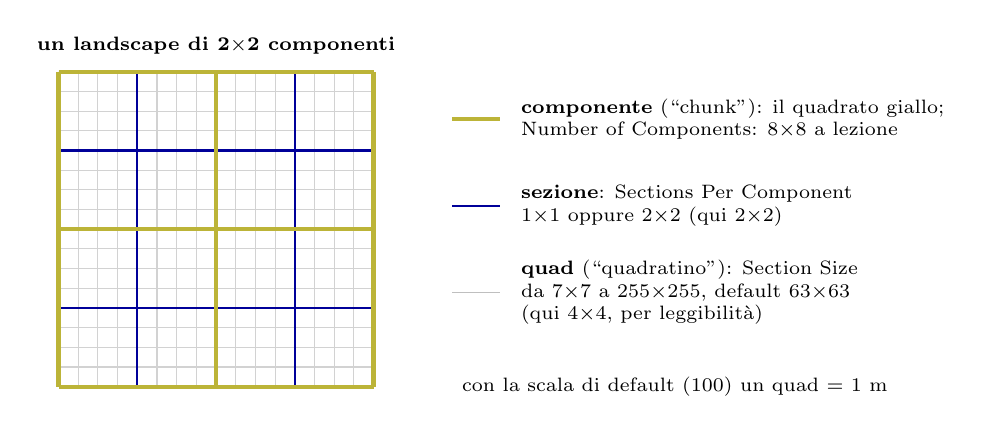
\begin{tikzpicture}[font=\footnotesize, x=1cm, y=1cm]
  % landscape 2x2 componenti, ognuno 2x2 sezioni, sezioni 4x4 quad (schematico)
  \begin{scope}
    \draw[gray!35, step=0.25] (0,0) grid (4,4);
    \draw[blue!60!black, thick, step=1] (0,0) grid (4,4);
    \draw[yellow!70!black, ultra thick, step=2] (0,0) grid (4,4);
    \node[anchor=south, font=\scriptsize\bfseries] at (2,4.1) {un landscape di 2$\times$2 componenti};
  \end{scope}
  % legenda
  \begin{scope}[xshift=5cm]
    \draw[yellow!70!black, ultra thick] (0,3.4) -- (0.6,3.4);
    \node[anchor=west, align=left, font=\scriptsize] at (0.75,3.4) {\textbf{componente} (``chunk''): il quadrato giallo;\\Number of Components: 8$\times$8 a lezione};
    \draw[blue!60!black, thick] (0,2.3) -- (0.6,2.3);
    \node[anchor=west, align=left, font=\scriptsize] at (0.75,2.3) {\textbf{sezione}: Sections Per Component\\1$\times$1 oppure 2$\times$2 (qui 2$\times$2)};
    \draw[gray!50] (0,1.2) -- (0.6,1.2);
    \node[anchor=west, align=left, font=\scriptsize] at (0.75,1.2) {\textbf{quad} (``quadratino''): Section Size\\da 7$\times$7 a 255$\times$255, default 63$\times$63\\(qui 4$\times$4, per leggibilità)};
    \node[anchor=west, align=left, font=\scriptsize] at (0,0.0) {con la scala di default (100) un quad = 1 m};
  \end{scope}
\end{tikzpicture}
\caption{La struttura di un landscape. I componenti (i \emph{chunk} gialli della preview)
sono le unità che il motore gestisce separatamente; ogni componente è diviso in una o
quattro sezioni; ogni sezione è una griglia di quad. Più quad significano curve più
morbide e più peso. Schema con valori ridotti per leggibilità.}
\label{ue14:fig:struttura}
\end{figure}

\begin{table}[htbp]
\centering
\small
\begin{tabular}{@{}p{4.2cm}p{3.0cm}p{6.8cm}@{}}
\toprule
\textbf{Parametro} & \textbf{A lezione} & \textbf{Che cosa decide} \\
\midrule
Section Size & 63$\times$63 (default); provati 31$\times$31 e 7$\times$7 & quanti quad ha
ogni sezione: più quad, terreno più morbido e più pesante \\
Sections Per Component & 2$\times$2, poi 1$\times$1 & in quante sezioni è diviso ogni
componente \\
Number of Components & 8$\times$8 & quanti componenti sulle X e sulle Y (landscape lungo,
largo, quadrato) \\
Overall Resolution & ricalcolata & il numero totale di vertici per lato (deriva dai valori
sopra) \\
Location, Rotation, Scale & invariati & la posizione e la dimensione del landscape; la scala
cambia la dimensione dei quad \\
Material & rimandato & il materiale con cui il landscape nasce \\
Fill World & non usato & crea un landscape grande quanto il mondo \\
Edit Layers & visti nella Manage & i livelli di modifica sovrapposti, bloccabili \\
\bottomrule
\end{tabular}
\caption{I parametri di creazione del landscape visti a lezione.}
\label{ue14:tab:creazione}
\end{table}

\paragraph{Approfondimento: i numeri del landscape di default.} Un quad, con la scala di
default (100 su X e Y), misura un metro: è comodo, perché la griglia del terreno coincide
con quella del pavimento della gym. La \emph{Overall Resolution} è il numero di vertici per
lato: con sezioni di 63 quad, una sezione per componente e 8 componenti per lato si hanno
$8 \times 63 + 1 = 505$ vertici, cioè un landscape di 504 metri per lato; con 2$\times$2
sezioni per componente il conto raddoppia ($8 \times 126 + 1 = 1009$). Le dimensioni
ammesse sono quelle della forma $2^n-1$ (7, 15, 31, 63, 127, 255) perché ogni livello di
LOD dimezza i quad di una sezione. Il componente è l'unità che il motore disegna, scarta e
semplifica: componenti più grandi significano meno oggetti da gestire ma un controllo più
grossolano. Epic consiglia di non esagerare con il numero di componenti (qualche migliaio
al massimo) e di scegliere le dimensioni fra quelle raccomandate nella documentazione. I
\emph{layer} della scheda Manage sono gli \textbf{Edit Layers}, attivi di default in
Unreal Engine~5: ogni layer conserva le proprie modifiche di scultura e di pittura, si può
bloccare, nascondere o cancellare senza toccare gli altri, come in un programma di grafica.
Funzionamento generale dell'engine.

% ---------------------------------------------------------------------
\section{Il pennello: falloff, strength, Alpha e Pattern}
\label{ue14:sec:pennello}

Lo strumento con cui si modifica il landscape ``è un cerchio, un pennello''. Cliccando, il
terreno si alza nel punto evidenziato: ``perché si alza? Perché siamo su \textbf{Sculpt} come
tool''. Prima degli strumenti, però, il docente spiega il pennello, che ``lascia anche
questa specie di immagine residua quando passa'' e ha una serie di parametri comuni a quasi
tutti gli strumenti (tabella~\ref{ue14:tab:pennello}).

\paragraph{Size, Falloff e Strength.}
\begin{itemize}
  \item la \textbf{grandezza} del pennello (\emph{Brush Size}), ``quindi effettivamente quanto è
        largo'';
  \item il \textbf{falloff}: ``è la distanza che c'è fra il primo cerchio e il secondo
        cerchio''. Il pennello ha due cerchi concentrici: dentro il primo l'effetto è pieno,
        fra il primo e il secondo sfuma. Con falloff \textbf{0} ``è tutto pieno'', e quando si
        alza qualcosa ``si alza tutto in blocco''; con falloff \textbf{1} ``si alza solo la
        punta e il resto è tutto quanto ammorbidito, è tutta sfumatura'';
  \item la \textbf{strength} (\emph{Tool Strength}), ``la forza del tool'': a 0,1 l'effetto si
        applica lentamente, a 1 molto più in fretta. ``È quanto forte viene applicato lo
        strumento.''
\end{itemize}

\paragraph{I quadratini e lo stretch del materiale.} ``Cosa stiamo vedendo con questi
quadratini a terra?'' La griglia disegnata sul landscape mostra ``il modo in cui sono
strutturati i poligoni'' e quindi, ``di conseguenza, in che modo verrà \textbf{stretchato il
materiale} quando ce l'andiamo a mettere sopra''. Il docente confronta tre zone
(figura~\ref{ue14:fig:stretch}): in piano ``il massimo della fedeltà, della risoluzione''; su
una salita morbida un materiale ``stretchato mediamente, ma rimane compatto''; su una parete
alzata con falloff zero un materiale che ``esplode'', perché il terreno non sale ``dritto per
dritto verticale'': c'è un quad che viene tirato in verticale ``per far sì che un lato sia
sul livello superiore, l'altro lato sul livello inferiore'', e lì il materiale ``sarà tutto
rovinato''.

\paragraph{Le forme del falloff.} Il \emph{Brush Falloff} ha quattro forme
(figura~\ref{ue14:fig:falloff}):
\begin{itemize}
  \item \textbf{Smooth}: ``il fall off è morbido'';
  \item \textbf{Linear} (``sharp linear''): ``non è morbido, ma è lineare, è geometrico'', una
        linea ``che dritta per dritta parte dalla base e arriva verso l'alto'';
  \item \textbf{Spherical}: ``un effetto più bombato'', ``una sorta di collinetta'' che poi
        ``spiove verso il basso'';
  \item \textbf{Tip}, ``il fall off convesso'', l'opposto dello spherical: la base è morbida e
        poi diventa lineare, con un effetto che ricorda ``le montagne dell'isola di Drum'' di
        \emph{One Piece} (``Drummond Island'' nella trascrizione: sono i \emph{Drum
        Rockies}, montagne a colonna).
\end{itemize}
``A seconda della situazione utilizzerete lo strumento più adatto'': linee morbide con lo
spherical, forme più aguzze con il tip.

\paragraph{I Brush Type.} ``Di base, il brush è un semplice \textbf{cerchio}''
(\emph{Circle}). Ma ci sono altri tipi:
\begin{itemize}
  \item l'\textbf{Alpha}: ``ora il nostro pennello non è più un cerchio, è una
        \textbf{texture}''. Si sceglie la texture dalla lista e ``funziona esattamente come
        avevamo fatto per i materiali: ci sono degli 0 e degli 1'': il pennello alza i bianchi
        e lascia a terra i neri. Con una texture di prova fatta di due quadrati bianchi e due
        neri si vede bene; il pennello \textbf{ruota} seguendo il movimento perché è attivo
        l'\emph{Auto Rotate}, che si può disattivare. L'uso tipico è con le texture di
        \textbf{noise}, che creano ``disturbo'': troppo, se esagerato, ma ``può esservi utile
        per andare a creare un effetto montagnoso, zigrinato, che dalla distanza può essere
        piacevole alla vista''. Qui si possono cambiare solo la grandezza e poco altro;
  \item il \textbf{canale} della texture (\emph{Texture Channel}), disponibile sia nell'Alpha
        sia nel Pattern. Il docente ripassa i canali, visti ``alla prima lezione che avevo
        fatto'': una texture ha i canali \textbf{RGB}, e i grafici li usano ``per mettere più di
        un'informazione all'interno della stessa texture'', come nelle mappe \textbf{ORM}
        (\emph{ambient occlusion} nel rosso, \emph{roughness} nel verde, \emph{metallic} nel
        blu). Il pennello può usare solo il rosso, solo il verde o solo il blu; con il noise
        ``saranno tutte uguali'';
  \item il \textbf{Pattern}: ``un portare all'estremo quello che faceva l'alfa''. La texture
        non è più ``messa su un quadrato'' ma proiettata sotto un pennello circolare, ``una
        fusione delle due precedenti'', e si può modificare: la \textbf{scala} (più piccola,
        ``molta più differenza nella costruzione''), la \textbf{rotazione}, le \textbf{U} e le
        \textbf{V}, ``quindi il \emph{panning}'', cioè lo scorrimento della texture.
        L'esempio: ``la faccia di Marte'', la collina che sembra un volto: con una texture a
        forma di faccia ``sembra che il terreno sia costruito in forma di faccia'';
  \item il \textbf{Component}, ``che io non ho mai usato, per essere onesto'': lavora
        direttamente sui componenti, per esempio per alzare un singolo chunk. Utile per
        dividere il landscape in due zone, ``una zona superiore e una zona inferiore'', che il
        giocatore dovrà collegare ``facendo X cose''.
\end{itemize}

\begin{figure}[htbp]
\centering
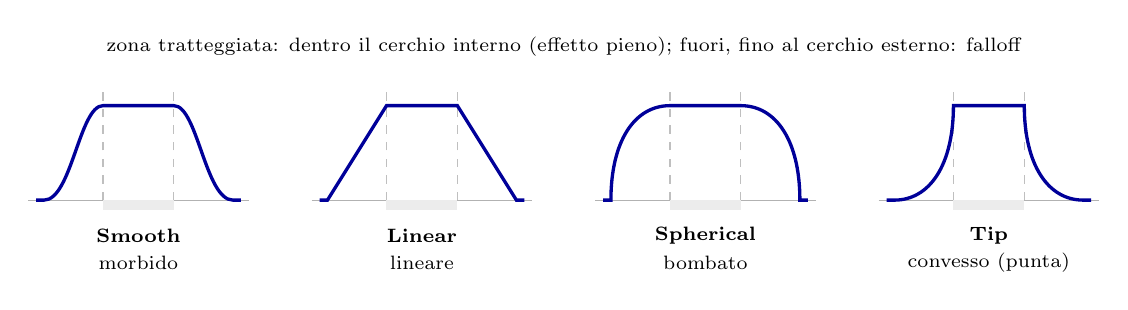
\begin{tikzpicture}[font=\footnotesize, x=1cm, y=1cm]
  \foreach \i/\name/\desc in {0/Smooth/morbido, 1/Linear/lineare, 2/Spherical/bombato, 3/Tip/convesso (punta)} {
    \begin{scope}[xshift=\i*3.6cm]
      \draw[gray!60] (-1.4,0) -- (1.4,0);
      \fill[gray!15] (-0.45,-0.12) rectangle (0.45,0);
      \draw[gray!50, dashed] (-0.45,0) -- (-0.45,1.4) (0.45,0) -- (0.45,1.4);
      \node[font=\scriptsize\bfseries] at (0,-0.45) {\name};
      \node[font=\scriptsize] at (0,-0.8) {\desc};
    \end{scope}
  }
  % Smooth: cosine
  \draw[very thick, blue!60!black] (-1.3,0) -- (-1.2,0) .. controls (-0.85,0) and (-0.75,1.2) .. (-0.45,1.2) -- (0.45,1.2) .. controls (0.75,1.2) and (0.85,0) .. (1.2,0) -- (1.3,0);
  % Linear
  \begin{scope}[xshift=3.6cm]
    \draw[very thick, blue!60!black] (-1.3,0) -- (-1.2,0) -- (-0.45,1.2) -- (0.45,1.2) -- (1.2,0) -- (1.3,0);
  \end{scope}
  % Spherical
  \begin{scope}[xshift=7.2cm]
    \draw[very thick, blue!60!black] (-1.3,0) -- (-1.2,0) .. controls (-1.2,0.75) and (-0.9,1.2) .. (-0.45,1.2) -- (0.45,1.2) .. controls (0.9,1.2) and (1.2,0.75) .. (1.2,0) -- (1.3,0);
  \end{scope}
  % Tip
  \begin{scope}[xshift=10.8cm]
    \draw[very thick, blue!60!black] (-1.3,0) -- (-1.2,0) .. controls (-0.75,0) and (-0.45,0.45) .. (-0.45,1.2) -- (0.45,1.2) .. controls (0.45,0.45) and (0.75,0) .. (1.2,0) -- (1.3,0);
  \end{scope}
  \node[font=\scriptsize, align=center] at (5.4,1.95) {zona tratteggiata: dentro il cerchio interno (effetto pieno); fuori, fino al cerchio esterno: falloff};
\end{tikzpicture}
\caption{Le quattro forme del \emph{Brush Falloff}, viste in sezione dopo aver alzato il
terreno con lo stesso pennello. Smooth sfuma in modo morbido, Linear con una rampa
dritta, Spherical con una collinetta bombata che spiove all'esterno, Tip con una base
morbida e una punta ripida. Profili schematici.}
\label{ue14:fig:falloff}
\end{figure}

\begin{figure}[htbp]
\centering
\begin{tikzpicture}[font=\footnotesize, x=1cm, y=1cm]
  % profilo del terreno con griglia di quad (vista laterale)
  \draw[gray!50] (0,0) -- (12,0);
  % piano
  \foreach \x in {0,0.5,...,3.5} {\draw[thick, green!40!black] (\x,0) -- (\x+0.5,0); \fill[green!40!black] (\x,0) circle (0.04);}
  \node[font=\scriptsize, align=center] at (2,-0.6) {piano: quad regolari\\``massima fedeltà''};
  % salita morbida
  \draw[thick, orange!80!black] (4,0) -- (4.5,0.15) -- (5,0.4) -- (5.5,0.7) -- (6,0.95) -- (6.5,1.1) -- (7,1.15);
  \foreach \p in {(4,0),(4.5,0.15),(5,0.4),(5.5,0.7),(6,0.95),(6.5,1.1),(7,1.15)} {\fill[orange!80!black] \p circle (0.04);}
  \node[font=\scriptsize, align=center] at (5.5,-0.6) {salita morbida:\\stretch medio};
  % parete
  \draw[thick, red!70!black] (7,1.15) -- (7.5,1.15) -- (8,1.15) -- (8.5,3.0) -- (9,3.0) -- (9.5,3.0);
  \foreach \p in {(7.5,1.15),(8,1.15),(8.5,3.0),(9,3.0),(9.5,3.0)} {\fill[red!70!black] \p circle (0.04);}
  \draw[red!70!black, thick] (8,1.15) -- (8.5,3.0);
  \node[font=\scriptsize, align=center, red!70!black] at (10.6,2.1) {un solo quad tirato\\in verticale: il\\materiale ``esplode''};
  \draw[-{Stealth[length=2mm]}, red!70!black] (9.7,2.1) -- (8.35,2.1);
  % texture schematica sopra la parete
  \foreach \t in {0.15,0.3,...,0.9} {\draw[red!40] ($(8,1.15)!\t!(8.5,3.0)$) -- ++(0.12,0);}
  \node[font=\scriptsize, align=center] at (8.5,-0.6) {parete con falloff 0:\\stretch estremo};
  % smooth
  \draw[-{Stealth[length=2mm]}, thick, blue!60!black] (10.4,1.0) -- (11.6,1.0);
  \node[font=\scriptsize, align=center, blue!60!black] at (11.0,0.35) {Smooth:\\quad più\\proporzionati};
\end{tikzpicture}
\caption{Lo \emph{stretch} del materiale, visto di lato. I punti sono i vertici della
griglia del landscape, a distanza fissa in pianta: in piano i quad sono regolari, su una
salita morbida si allungano un po', su una parete alzata in blocco un solo quad copre tutto
il dislivello e la texture si stira fino a diventare illeggibile. Lo strumento Smooth
riavvicina le proporzioni. Ricostruzione schematica.}
\label{ue14:fig:stretch}
\end{figure}

\begin{table}[htbp]
\centering
\small
\begin{tabular}{@{}p{3.6cm}p{10.4cm}@{}}
\toprule
\textbf{Parametro} & \textbf{Che cosa fa} \\
\midrule
Brush Size & la grandezza del pennello \\
Brush Falloff & la parte sfumata fra il cerchio interno e quello esterno: 0 tutto pieno, 1
tutto sfumato \\
Tool Strength & quanto in fretta e quanto forte si applica l'effetto (0,1 lento, 1 forte) \\
Falloff: Smooth, Linear, Spherical, Tip & la forma della sfumatura: morbida, lineare,
bombata, convessa a punta \\
Brush Type: Circle & il pennello circolare di base \\
Brush Type: Alpha & una texture come pennello: alza i bianchi, lascia i neri; Auto Rotate
lo fa ruotare con il movimento \\
Texture Channel & quale canale della texture usare (R, G o B) \\
Brush Type: Pattern & una texture proiettata sotto il pennello circolare, con scala,
rotazione e panning U/V \\
Brush Type: Component & agisce su interi componenti \\
\bottomrule
\end{tabular}
\caption{I parametri del pennello del Landscape Mode, comuni a quasi tutti gli
strumenti di scultura e di pittura.}
\label{ue14:tab:pennello}
\end{table}

\paragraph{Approfondimento: perché la parete ``esplode''.} Il landscape, essendo un
\emph{heightfield}, ha i vertici a distanza fissa in pianta: alzare un punto ne cambia solo
l'altezza, non la posizione orizzontale. Un dislivello di dieci metri fra due vertici
distanti un metro produce un quad lungo più di dieci metri e largo uno, e la texture,
mappata di default dall'alto (proiezione planare sul piano XY), vi si stira di dieci volte.
I rimedi sono tre: evitare pendenze troppo ripide (lo Smooth, che il docente chiama ``il
miglior amico dei vostri materiali''), usare nel materiale una proiezione che tenga conto
delle pareti (la proiezione \emph{triplanare} o \emph{world aligned}, che il materiale
StackOBot usa con la Absolute World Position), oppure coprire le pareti verticali con
delle mesh di roccia, come si fa quasi sempre nelle produzioni reali. Funzionamento
generale dell'engine.

% ---------------------------------------------------------------------
\section{La domanda sulle caverne}
\label{ue14:sec:caverne}

``C'è qualcosa che volevi chiedere per ora? Prima dicevi delle caverne che non si possono
fare.'' Uno studente ha provato a smanettare: è \textbf{impossibile fare dei buchi nel
landscape} con questi strumenti. Il docente conferma: ``per fare un buco avete bisogno dello
strumento \textbf{Visibility}, della \textbf{visibility mask}''. Ma la visibility mask ``si
modifica dal materiale del landscape'': bisogna aggiungere al materiale dei nodi specifici,
e solo allora si potrà avere una parte di landscape attraversabile, ``in cui possiamo andare
a costruire delle caverne''.

Lo studente pensava ad \textbf{Astroneer}, in cui scavare il terreno è la meccanica
principale. Il docente distingue due logiche: ``quando vai a creare un gioco devi far sì che
l'editor per il giocatore sia più \emph{user friendly} possibile''; ``quando stai creando un
editor, forse ti preoccupi di avere più possibilità possibili a disposizione''. Il buco ``si
può fare, non si può fare da qui''. In anteprima mostra lo strumento Visibility: il pennello
è \textbf{rosso} e cliccando non fa nulla, perché in basso Unreal avverte che il
\emph{visibility painting} è disabilitato: il componente ``non ha il nodo \textbf{Landscape
Visibility Mask} nel materiale''. Lo si vedrà a fine lezione
(sezione~\ref{ue14:sec:visibility}).

\paragraph{Approfondimento: terreni scavabili.} Giochi come Astroneer non usano un
heightfield ma un terreno \emph{volumetrico} (voxel), in cui ogni punto dello spazio sa se è
pieno o vuoto, e la superficie viene ricostruita a ogni modifica: per questo vi si possono
scavare tunnel e caverne in gioco. Il landscape di Unreal non funziona così, e una grotta
si fa nascondendo una porzione di terreno con la Visibility e costruendo l'interno con
delle mesh. Per terreni scavabili in Unreal esistono plugin di terzi basati sui voxel.
Funzionamento generale dell'engine.

% ---------------------------------------------------------------------
\section{Gli strumenti di scultura: Sculpt, Erase, Smooth, Flatten}
\label{ue14:sec:sculpt}

``Cosa fanno i nostri pennellozzi?'' ``Ognuno di voi troverà il modo con cui si trova più
comodo a fare le cose''; il docente mostra solo che cosa fa ogni strumento della scheda
\textbf{Sculpt} (tabella~\ref{ue14:tab:sculpt}).

\paragraph{Sculpt.} ``Il più semplice delle cose semplici'': scolpisce, alza il terreno. Ma,
come si è visto ``diverse volte per sbaglio'', non va solo verso l'alto: \textbf{Shift +
clic sinistro} ``scava'', e crea ``delle zone interrate'', delle depressioni.

\paragraph{Erase.} Cancella: ``elimina tutte le modifiche che abbiamo fatto, che siano verso
l'alto o verso il basso''. (Dopo la pausa il docente nota che anche l'Erase rispetta il
falloff: cancella ``in maniera sfumata'' le parti che cadono nella sfumatura.)

\paragraph{Smooth.} ``Ammorbidisce. Immaginatevelo come uno strumento che crea
sfumature.'' Se il pennello prende sia una parte alta sia una parte bassa, cliccando ``crea
una discesa più morbida'': ``fa una media, alza le parti abbassate, abbassa le parti un
pochino più alte'' e produce una \emph{slope} più leggera. ``Lo strumento Smooth è il miglior
amico dei vostri materiali'': ricordando che quanto sono stirati i quadratini ``è anche quanto
saranno stretchati i materiali'', uno smoothing li rende ``sempre più proporzionati''. Con un
pennello più grande della cima, però, ``lui abbassa proprio tutto''; per i ``lavori di fino''
si rimpicciolisce il pennello e si fanno piccole modifiche ``che non vanno a sbragare
completamente tutta la parete''. Anche qui ci sono falloff, tipi di pennello e strength, e
un parametro in più per la \textbf{precisione} dello smoothing (il \emph{Detail Smooth}):
``più grande è questo valore, più dettagli vengono rimossi'', più piccolo, ``meno dettagli
vengono rimossi''. I ``dettagli'' sono ``tutti questi su e giù'': con un valore alto e un
pennello grande ``lui pialla tutto'', con un valore piccolo i cambiamenti sono ``molto
morbidi'' e ``molto precisi''; ``a zero chiaramente non farà mai nulla''.

\paragraph{Flatten.} ``Il mio strumento preferito.'' Il docente si costruisce ``un piccolo
parco giochi'' di colline per gli esempi. Il \textbf{Flatten} ``ci permette di selezionare un
punto e appiattire tutto quanto a quell'altezza'': si clicca dove c'è la croce e tutto ciò
che passa sotto il pennello viene portato a quell'altezza, sia in basso sia sulla vetta.
Serve a una ``terraformazione un po' più controllata'':
\begin{itemize}
  \item \textbf{plateau}, altopiani: il ``lenzuolo'' tirato su si interrompe al bordo,
        ``non riscende giù'';
  \item \textbf{scaloni}, cliccando su punti diversi di una slope: ``scalone, altro scalone,
        altro scalone'', ``delle formazioni un po' più sensate, un po' più normali'', da
        ammorbidire poi con lo Smooth. Per esempio ``le cascatine fatte a livelli'' o ``le
        \textbf{risaie}'', con parti piatte e parti rialzate;
  \item un \textbf{canyon} dentro una parte rialzata: un fondo appiattito e i lati rimasti
        alti.
\end{itemize}

\paragraph{Le modalità del Flatten.} ``È abbastanza brutale come strumento, perché prende e
appiattisce tutto'': si rischia di appiattire le cose sbagliate. Per questo c'è la
\textbf{Flatten Mode} (figura~\ref{ue14:fig:flatten}):
\begin{itemize}
  \item \textbf{Both} (default): ``alza i piani che stanno più in basso e abbassa i piani che
        stanno più in alto'';
  \item \textbf{Raise}: alza tutti i punti fino all'altezza scelta, ``però non abbassa''.
        Esempio: un rilievo che fa da \textbf{bordo della mappa} resta intatto, e si alza
        solo ciò che c'è sotto;
  \item \textbf{Lower}: abbassa ``tutto quello che c'è da abbassare, ma non alza'': ``se c'è
        una grotta o un canyon che deve rimanere giù, non lo tira più su''.
\end{itemize}
``Principalmente questi sono i due che vorrete utilizzare, perché sono quelli che vi danno
un po' più di controllo.'' Di un'altra opzione il docente legge a fatica il nome (``height
intervals'', ``specification at intervals''): ``questo è uno che effettivamente non ho mai
utilizzato''. Si tratta, con ogni probabilità, della modalità \textbf{Terrace} (si veda
l'approfondimento).

\paragraph{Use Slope Flatten.} Con la casella \textbf{Use Slope Flatten}, invece di
appiattire in orizzontale ``andate a continuare il piano diagonale preso originariamente'':
cliccando su un pendio, lo strumento prolunga quella pendenza, ``anche scavando verso il
basso''. Serve per ``quei pianori, quegli spiazzi montani'' che sono ``uno spaccato dritto per
dritto, che però va in diagonale''. Ultimo uso, personale: ``a volte il Flatten tendo a
utilizzarlo tipo \textbf{gomma}'': si punta sul livello base del landscape e si appiattisce.

``Abbiamo visto scolpire, tirare su, tirare giù, ammorbidire, cancellare e appiattire.''

\begin{figure}[htbp]
\centering
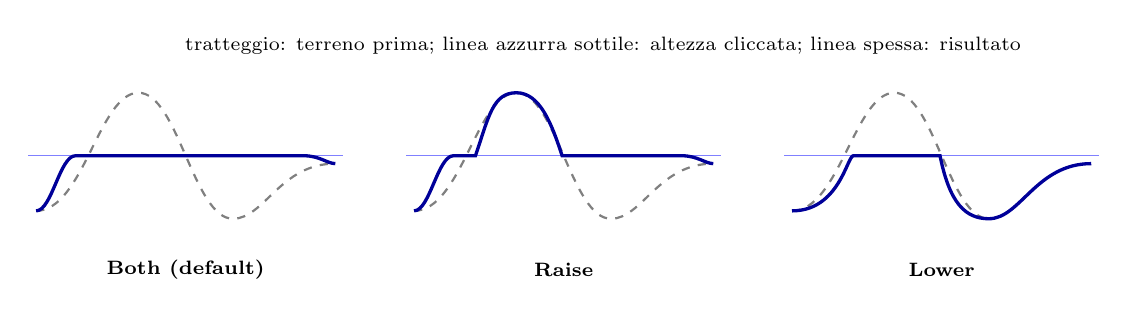
\begin{tikzpicture}[font=\footnotesize, x=1cm, y=1cm]
  \foreach \i/\name in {0/Both (default), 1/Raise, 2/Lower} {
    \begin{scope}[xshift=\i*4.8cm]
      % profilo originale
      \draw[gray, dashed, thick] (0,0.3) .. controls (0.6,0.3) and (0.8,1.8) .. (1.3,1.8) .. controls (1.8,1.8) and (2.0,0.2) .. (2.5,0.2) .. controls (2.9,0.2) and (3.1,0.9) .. (3.8,0.9);
      \draw[blue!50, thin] (-0.1,1.0) -- (3.9,1.0);
      \node[font=\scriptsize, blue!60!black, anchor=west] at (3.9,1.0) {};
      \node[font=\scriptsize\bfseries] at (1.9,-0.45) {\name};
    \end{scope}
  }
  % Both: tutto a 1.0
  \draw[very thick, blue!60!black] (0,0.3) .. controls (0.2,0.3) and (0.3,1.0) .. (0.5,1.0) -- (3.4,1.0) .. controls (3.6,1.0) and (3.7,0.9) .. (3.8,0.9);
  % Raise: alza le valli, non abbassa la cima
  \begin{scope}[xshift=4.8cm]
    \draw[very thick, blue!60!black] (0,0.3) .. controls (0.2,0.3) and (0.3,1.0) .. (0.5,1.0) -- (0.78,1.0) .. controls (0.95,1.5) and (1.0,1.8) .. (1.3,1.8) .. controls (1.6,1.8) and (1.75,1.4) .. (1.88,1.0) -- (3.4,1.0) .. controls (3.6,1.0) and (3.7,0.9) .. (3.8,0.9);
  \end{scope}
  % Lower: abbassa la cima, non alza le valli
  \begin{scope}[xshift=9.6cm]
    \draw[very thick, blue!60!black] (0,0.3) .. controls (0.6,0.3) and (0.7,1.0) .. (0.78,1.0) -- (1.88,1.0) .. controls (2.0,0.4) and (2.2,0.2) .. (2.5,0.2) .. controls (2.9,0.2) and (3.1,0.9) .. (3.8,0.9);
  \end{scope}
  \node[font=\scriptsize, align=center] at (7.2,2.4) {tratteggio: terreno prima; linea azzurra sottile: altezza cliccata; linea spessa: risultato};
\end{tikzpicture}
\caption{Le tre modalità principali del Flatten, in sezione. Both porta tutto all'altezza
cliccata; Raise alza solo ciò che sta sotto e lascia la cima (per esempio il bordo della
mappa); Lower abbassa solo ciò che sta sopra e lascia le valli (per esempio un canyon).
Profili schematici.}
\label{ue14:fig:flatten}
\end{figure}

\paragraph{Approfondimento: Terrace e gli altri parametri del Flatten.} Nella versione di
Unreal Engine~5 il Flatten ha quattro modalità: oltre a Both, Raise e Lower, la modalità
\textbf{Terrace}, che appiattisce il terreno a \emph{intervalli} di altezza regolari
(\emph{Terrace Interval}), con una sfumatura fra un gradino e l'altro (\emph{Terrace
Smooth}): è lo strumento giusto per le risaie e le cascate a livelli che il docente
costruisce a mano cliccando su più punti. Altri parametri utili: \emph{Pick Value Per
Apply}, che ricampiona l'altezza a ogni pennellata invece di tenere quella del primo clic;
\emph{Flatten Target}, che permette di scrivere a mano l'altezza a cui appiattire (comodo
per avere esattamente le misure della gym, per esempio un plateau a 1,40 m sopra un
altro); e \emph{Show Preview Grid}, che mostra il piano di destinazione. Funzionamento
generale dell'engine; la lezione non li tocca.

% ---------------------------------------------------------------------
\section{Ramp e i LOD}
\label{ue14:sec:ramp}

``Adesso vediamo uno strumento che funziona in maniera un po' diversa. Non è più un
pennello, ma dei clic'': lo strumento \textbf{Ramp}. Si clicca su due punti, li si sposta
come si vuole, e quando si è contenti si preme \textbf{Add Ramp}: Unreal aggiunge ``un
collegamento di landscape da punto A a punto B''. Il docente chiede alla classe che cosa
succederà con due punti sul fondo di due valli separate da una collina: ``ti farà un canyon
lì in mezzo'' (la rampa porta il terreno ``sempre da punto A a punto B'', anche scavando).

\paragraph{Gli usi.}
\begin{itemize}
  \item una \textbf{rampa} per salire su un punto sopraelevato (``sarà un modo molto brutto,
        però va'');
  \item le rampe di un gioco di \textbf{macchine} o di \textbf{skateboard};
  \item ``una \textbf{diga} in un crepaccio'', un collegamento pieno da una parte all'altra.
\end{itemize}
Un \textbf{ponte sospeso}, invece, no. Si potrebbe pensare di fare la diga e poi bucarla
sotto con la Visibility, ``tuttavia ci sarebbe un problema'': la parte sotto non
collegherebbe più le due metà, ``perché il landscape \textbf{non può essere sovrapposto}'',
``non può esserci una parte qui e una parte sotto''. ``Se volete fare un ponte sospeso,
fatelo con le \textbf{mesh}: prendete una mesh, ingranditela e mettetela sopra un crepaccio.
Non fatelo con il landscape.''

\paragraph{Larghezza e falloff.} La rampa ha la sua \textbf{larghezza} (\emph{Ramp Width}),
``se un ponticello, se una grossa salita'', e il suo \textbf{falloff} (\emph{Side Falloff}):
a zero non c'è sfumatura e i lati vengono stirati ``a blocco''; tutto sfumatura, e il
terreno attorno si raccorda morbido. Ma se si ``tira la corda'', con molta sfumatura e una
rampa molto stretta, ``vi si spacca un po' il landscape'': ``questa cosa è molto rotta, e
dalla distanza sarà tremenda'', ``perché i \textbf{LOD} vanno a semplificare il landscape''.

\paragraph{I LOD.} ``Sapete che cos'è un LOD?'' \textbf{LOD} sta per \emph{Level of Detail}.
Un grafico crea una mesh, poniamo da 10.000 poligoni; questa mesh deve avere ``altre
versioni di sé più grezze'', da 5.000, da 2.000 poligoni, perché l'engine, ``e non solo in
automatico'', aggiorna il numero di poligoni ``a seconda della distanza da cui lo vedi''.
L'esempio della statua: da vicino deve essere ``super bellissima'', ma da lontano ``non serve
che abbia ancora 500.000 poligoni'', perché l'occhio non vedrà il dettaglio, e ridurli
alleggerisce le prestazioni. Le distanze si possono impostare (``a 10 metri un tot, a 20
metri un altro tot, a 40 metri un altro tot''), da un Blueprint o dalla mesh stessa. Il
landscape funziona allo stesso modo: dalla distanza i suoi poligoni vengono semplificati.
Una massa grande non ne soffre, ``perché ci sono molti poligoni''; una rampa sottilissima,
``costituita di troppi pochi poligoni, viene distrutta dai LOD''. ``Quindi evitate di fare
delle robe in questo modo.''

\paragraph{Lo sfogo sui Pokémon.} L'esempio, dichiaratamente polemico: i recenti Pokémon
open world, \emph{Scarlatto e Violetto} e \emph{Leggende Pokémon: Arceus}. ``Potete vedere
attivamente la terra che si muove, come se fosse animata'': ``sono semplicemente i LOD che si
attivano troppo presto'', il landscape ``viene semplificato con troppo anticipo''. Il
motivo, secondo il docente, è l'ottimizzazione: se in una visione ampia si vedesse tutto
con tutti i poligoni ``esploderebbe la console''. ``Non è che sono brutte, ma è che sono
troppo ottimizzate, e la troppa ottimizzazione le rende orribili''; e sono così ottimizzate
``perché il gioco è programmato in maniera talmente stupida da essere pesante''. ``Scusate
questo piccolo sfogo contro Game Freak.'' (È un giudizio personale del docente, non
un'analisi tecnica verificata; il fenomeno del terreno che ``si muove'' quando cambia il LOD,
il \emph{LOD popping}, è comunque reale e ben noto.)

\paragraph{La regola.} ``Diamo sempre un po' di spazio al landscape'': niente forme troppo
sottili. ``Questo è anche il motivo per cui vorremmo evitare dei landscape troppo piccoli'':
un landscape 7x7 ``capita molto spesso che si spacchi in questo modo, perché ha pochi
poligoni a disposizione''. Il docente rifà ``una rampina decente''.

\paragraph{Approfondimento: i LOD del landscape.} Il landscape non ha LOD costruiti a mano
come una static mesh: li calcola da solo, dimezzando a ogni livello i quad di ogni sezione
(per questo le Section Size sono della forma $2^n-1$). La transizione è regolata da
parametri dell'actor Landscape (in Unreal Engine~5 \emph{LOD 0 Screen Size}, \emph{LOD 0
Distribution Setting} e \emph{LOD Distribution Setting}, più eventuali \emph{LOD Group}),
che decidono a quale dimensione sullo schermo un componente passa al livello successivo.
Aumentarli rende il terreno lontano più fedele e più costoso. Le forme più sottili di una
sezione, come la rampa stretta del docente, sono le prime a sparire perché nel livello
semplificato non ci sono più vertici abbastanza vicini per descriverle. Il capitolo 12 di
Romero e Sewell, sulla pubblicazione, ricorda che fra le impostazioni di scalabilità del
gioco c'è anche la qualità del \emph{foliage}, e che se le prestazioni calano solo in certe
zone del livello conviene ``ridurre la densità degli oggetti'' o la qualità di un modello:
il compromesso fra dettaglio e prestazioni di cui parla il docente. Per la parte sui
parametri del landscape, funzionamento generale dell'engine.

% ---------------------------------------------------------------------
\section{Erosion, Hydro, Noise, Mirror e Copy/Paste}
\label{ue14:sec:altristrumenti}

\paragraph{Erosion e Hydro.} ``Sono due strumenti con cui io faccio un po' a botte'' (``a
volte'' nella trascrizione, ma il seguito chiarisce il senso): il
docente spiega a che cosa servirebbero e perché non gli piacciono. L'idea è ``simulare
delle deformazioni, del \emph{displacement}''. L'\textbf{Erosion} è lo strumento con cui
``andrei a dettagliare una parete montuosa'': ``è un po' il contrario dello smooth'', crea
nel pennello parti rialzate e parti abbassate. (Qui la trascrizione si interrompe in una
frase ripetuta; riprende con la domanda di uno studente.)
\begin{itemize}
  \item il \textbf{Threshold} ``va a definire quanta differenza fra punto A e punto B deve
        esserci per andare a fare erosione'': con un valore alto l'erosione si applica solo
        dove il dislivello è grande; abbassandolo (``tipo 17'') si erode ``molto di più, in
        molti punti diversi'', perché basta una differenza minore;
  \item \textbf{Noise Mode} e \textbf{Noise Scale} aggiungono un rumore preimpostato, e come
        nel Flatten si sceglie se deve alzare e abbassare, solo alzare o solo abbassare.
\end{itemize}
L'\textbf{Hydro} (\emph{Hydro Erosion}) ``funziona più o meno nello stesso modo'' e
vorrebbe creare un \emph{displacement} ``stile fondali marini'' o ``erosione dell'acqua''. Il
problema è che ``abbiamo un po' poco controllo'': ``io non sono mai riuscito a farlo
funzionare bene, proprio non mi trovo''.

\paragraph{Noise.} ``Preferisco piuttosto utilizzare il \textbf{Noise}'', che ``fa rumore'' e
permette di scegliere se aggiunge, se toglie o se fa entrambe le cose. Con un pennello
grande e la scala del noise ridotta, ``vi va a fare una deformazione un po' più subdola'':
``non prende e spacca, ma fa dei leggeri movimenti di alzare e abbassare'', il risultato
``che al mio occhio è sempre il più piacevole''. In modalità solo-aggiunta il Noise alza,
``però non come lo Sculpt'' (aggiunge rumore, non una collina); lo stesso vale per la
sottrazione.

\paragraph{Gli strumenti saltati.} ``Facciamo al volissimo le ultime cose'':
\begin{itemize}
  \item il \textbf{Retopologize} ``non ci interessa'';
  \item la \textbf{Visibility}, già vista, si riprende più avanti;
  \item il \textbf{Blueprint Brush}, ``qualcosa che onestamente non ho mai utilizzato'':
        ``presumo sia un brush che può essere programmato'' per fare cose specifiche. ``Non
        l'ho mai trovato necessario.''
\end{itemize}

\paragraph{Mirror.} Il \textbf{Mirror} serve ``nel momento in cui avete degli ambienti molto
grandi che volete copiare, che volete specchiare o che volete ruotare''. Compare un
\textbf{piano}: premendo \textbf{Apply}, tutto ciò che sta da un lato viene copiato
sull'altro, ``appiattendo'' quello che c'era. Il piano si sposta avanti e indietro, e
soprattutto dall'\textbf{Operation} si sceglie il tipo di operazione:
\begin{itemize}
  \item \textbf{-X to +X}: copia il lato sinistro sul destro; \textbf{+X to -X} il contrario;
        lo stesso per \textbf{-Y to +Y} e \textbf{+Y to -Y}. Con una forma qualsiasi si ottiene
        ``una macchia di Rorschach'';
  \item le varianti \textbf{Rotate} (per esempio \emph{Rotate -X to +X}): stessa direzione del
        piano, ``ma operazione diversa'': invece di specchiare, ruota, ``come se prendesse
        questa parte del landscape e la ruotasse nell'altra direzione''. Il risultato è
        uguale, ``ma ruotato''.
\end{itemize}

\paragraph{Copy/Paste.} ``Il copia e incolla, la cosa più semplice del mondo.'' Prima si
seleziona una parte di landscape con lo strumento \textbf{Region Select} (``Select''),
dipingendo la zona con il pennello; per togliere la selezione serve \textbf{Clear Region
Selection}, ``perché se andate da altre parti questo vi rimane sempre selezionato''. Poi,
nello strumento \textbf{Copy/Paste}, \textbf{Ctrl+C} copia la zona in un riquadro (il
\emph{gizmo}) che si può spostare, ruotare e scalare dove si vuole, e \textbf{Ctrl+V} la
incolla, ``modificata, ruotata e anche scalata''. Ci sono comandi per adattare il riquadro
alla selezione e per ripulirlo. La \textbf{Paste Mode} ripete la logica del Flatten:
\begin{itemize}
  \item \textbf{Both}: tutto il riquadro viene portato al livello copiato, la zona di
        destinazione viene abbassata a livello base e la parte copiata rialzata;
  \item \textbf{Raise}: alza soltanto ``le parti che erano più basse'' e non abbassa le altre:
        di una collina copiata sopra un'altra resta solo ``la punta'';
  \item \textbf{Lower}: l'opposto.
\end{itemize}
``Abbiamo effettivamente un po' tutte le cose viste.'' Nessuna domanda: pausa, ``ci becchiamo
alle 55 con il Paint, e quindi i materiali del landscape''.

\begin{table}[htbp]
\centering
\small
\begin{tabular}{@{}p{3.0cm}p{11.0cm}@{}}
\toprule
\textbf{Strumento (Sculpt)} & \textbf{Che cosa fa, e come lo usa il docente} \\
\midrule
Sculpt & alza il terreno; Shift + clic scava \\
Erase & cancella le modifiche (rispetta il falloff) \\
Smooth & fa una media delle altezze; Detail Smooth decide quanto dettaglio togliere; ``il
miglior amico dei materiali'' \\
Flatten & appiattisce all'altezza cliccata; Flatten Mode Both, Raise, Lower (e Terrace);
Use Slope Flatten prolunga il pendio; usato anche come ``gomma'' \\
Ramp & crea una rampa fra due punti (Add Ramp), con Ramp Width e Side Falloff; non per i
ponti sospesi \\
Erosion & dettaglia le pareti erodendo dove il dislivello supera il Threshold; Noise Mode e
Noise Scale; ``poco controllo'' \\
Hydro (Hydro Erosion) & erosione ``ad acqua''; il docente non lo usa \\
Noise & aggiunge o toglie rumore; con scala piccola, deformazioni ``subdole'' \\
Retopologize & non visto (``non ci interessa'') \\
Visibility & nasconde porzioni di terreno; richiede la Landscape Visibility Mask nel
materiale \\
Blueprint Brush & pennelli programmabili; mai usato dal docente \\
Mirror & specchia (-X to +X, \dots) o ruota (Rotate \dots) metà del landscape; Apply \\
Region Select & seleziona una zona col pennello; Clear Region Selection \\
Copy/Paste & Ctrl+C e Ctrl+V di una zona, con gizmo spostabile, ruotabile, scalabile;
Paste Mode Both, Raise, Lower \\
\bottomrule
\end{tabular}
\caption{Gli strumenti della scheda Sculpt del Landscape Mode, nell'ordine della lezione.}
\label{ue14:tab:sculpt}
\end{table}

\paragraph{Approfondimento: il terreno come spazio di gioco.} Gli strumenti di scultura
sono tecnici, ma le forme che producono sono categorie di level design. Totten, nel
capitolo 3, osserva che in un open world fatto di paesaggi aperti, come \emph{Skyrim}, i
percorsi fra città e dungeon ``sono molto meno diretti'' e spesso ``campi aperti'': il
giocatore traccia da sé le scorciatoie fra i landmark, ma ``rischia di perdersi'', e i
designer usano ``elementi geografici sottili come sentieri sterrati, cartelli o fiumi'' per
suggerire i percorsi. E aggiunge proprio a proposito degli ``editor di terreno integrati
nell'engine'': tenere a mente queste linee guida serve a creare mondi ``non solo
esteticamente attraenti, ma anche utilizzabili''. Il canyon del Flatten, la diga della Ramp
e il bordo di mappa preservato dal Raise sono, in questi termini, un percorso, un
collegamento e un \emph{edge}; il plateau è un'area in cui il giocatore guarda lontano (il
\emph{prospect space} dello stesso capitolo). Le misure, infine, vengono dalla gym: un
canyon che deve essere invalicabile avrà pareti oltre il Walkable Floor Angle del
personaggio, un plateau raggiungibile con un salto starà sotto l'altezza comoda misurata.

% ---------------------------------------------------------------------
\section{La pausa e la domanda su The Sims}
\label{ue14:sec:pausa}

Alla ripresa (``Guido c'è, Federico c'è, Giulia c'è'') il docente chiede se sia tutto
chiaro: ``è abbastanza semplice, è più una questione di prenderci la mano''. Consiglia di
usare il landscape ``fra questa lezione e la prossima'' per familiarizzare e trovare il
proprio modo di lavorare: ``magari siete dei pazzi completi e lavorate utilizzando soltanto
lo Sculpt, ma siete fortissimi. Io vi dico quali sono i tool, poi voi trovate il vostro
modo di lavoro''.

\paragraph{The Sims.} Uno studente chiede se il terreno della serie \textbf{The Sims}, ``soprattutto
del 2'', sia fatto allo stesso modo. Il docente non lo sa: ``non so con cosa è stato fatto''.
Dopo un rapido controllo: ``a quanto risulta, ogni The Sims ha usato un \textbf{engine custom}''.
È ``plausibile'' che funzioni in modo simile, e che ci sia stata ``una \emph{cross
contamination}, delle influenze da entrambe le parti'': magari anche Unreal si è ispirato a
come ``diversi tycoon o diversi simulatori'' gestivano la terraformazione, perché ``quel tipo
di modifica spaziale è molto comodo farla con un pennello''. ``Non ti so dire di più'':
l'ultima volta che ha giocato a The Sims ``probabilmente era vent'anni fa''. Lo invita a fare
una ricerca e a riferire la volta successiva. (Nello scambio, alla domanda ``quando è uscito
The Sims 2?'', la risposta è ``nel 2000'': in realtà nel 2000 è uscito il primo
\emph{The Sims}; \emph{The Sims 2} è del 2004.)

% ---------------------------------------------------------------------
\section{Il Paint e il materiale del landscape di StackOBot}
\label{ue14:sec:paint}

``Abbiamo visto il Manage, abbiamo visto lo Sculpt, rimane soltanto da vedere il
\textbf{Paint}.'' La scheda ha ``più o meno gli stessi strumenti che c'erano di là'':
\textbf{Paint}, \textbf{Smooth}, \textbf{Flatten} e \textbf{Noise}, con la stessa strength e
gli stessi tipi di pennello. Ma in basso Unreal avverte: \emph{non ci sono target layer
assegnati a questo landscape; usa i bottoni in alto per aggiungerne di nuovi o popolarli
dal materiale correntemente assegnato}. I bottoni sono \textbf{Create Layer} e
\textbf{Create Layers from Assigned Materials}, quest'ultimo, ``se non sbaglio, unico di
Unreal 5, sulla quarta edizione non c'è''.

\paragraph{Un materiale normale non basta.} Il landscape può \textbf{dipingere il materiale}
con il pennello, ``il materiale però deve essere fatto \emph{ad hoc}''. Prova: un nuovo
materiale con dentro ``unicamente un colore''. Messo sul landscape, il landscape lo tratta
``come un oggetto qualsiasi'': ``tutto quanto diventa disgustosamente verde'', e non c'è modo
di modificare nulla, ``perché il nostro materiale di layer non ne ha''.

\paragraph{Il ``grosso errore''.} A questo punto il docente si accorge di ``aver fatto un grosso
errore: niente di grave, semplicemente una cosa che ci farà perdere un po' di tempo'' (la
spiegherà più avanti: sono le Virtual Texture, sezione~\ref{ue14:sec:grass}).

\paragraph{Il pacchetto StackOBot.} Fra gli asset del pacchetto \textbf{StackOBot}, ``il
pacchettino con il robottino e tutte le cose'', nella cartella \emph{Environment} ci sono:
\emph{Props} e \emph{Modular} (mesh da vedere alla fine della lezione ``o all'inizio della
prossima''), \emph{Materials}, \emph{Foliage} (per il Foliage Mode) e \textbf{Landscape}, con
``tutto quello che riguarda il landscape'': delle texture ``che non sappiamo bene cosa
fanno'', una mesh che per ora non serve, dei materiali, fra cui \textbf{M\_Landscape}, e dei
\textbf{Landscape Layers} ``che non sappiamo bene cosa fanno'' e che si rivedranno più
tardi.

\paragraph{Il nero.} Si assegna M\_Landscape al landscape (nel campo \emph{Landscape
Material} dei Details): ``va tutto \textbf{nero}''. Anche un materiale pensato per il
landscape, appena assegnato, ``non ci dà subito quello di cui abbiamo bisogno''; e ``il fatto
che diventi tutto nero è quello che vogliamo, per noi è positivo''. Bisogna stabilire come
funzionano i layer: visto che il materiale ``è già stato costruito per avere tanti layer
diversi'', si preme \textbf{Create Layers from Assigned Materials}. Unreal crea
\textbf{quattro layer}, e il terreno resta nero. (Resta nero perché nessun layer è ancora
stato dipinto: si veda l'approfondimento.)

\paragraph{Dentro M\_Landscape.} Il docente apre il materiale, ``molto piccolo, vero?
Molto comodo'' (ironico: il nodo principale è ridotto a un solo pin). Le parti interessanti:
\begin{itemize}
  \item quattro \textbf{material function}, \emph{MF\_Rocks}, \emph{MF\_Pebbles},
        \emph{MF\_Sand} e \emph{MF\_Grass}: ``il funzionamento dei singoli materiali, quindi
        dei singoli layer''. Si creano con tasto destro, \emph{Material Function}: sono
        ``delle piccole funzioni'', come quelle dei Blueprint, che descrivono ``come funziona
        l'erba, come funziona la ghiaia, i \emph{pebbles}'', la roccia e la sabbia;
  \item dentro ogni funzione le texture sono collegate alla \textbf{Absolute World
        Position}: ``vi ricordate i materiali \textbf{world aligned} che avevamo visto la
        volta scorsa? Questo è il modo per farli, anche per il landscape'';
  \item tutte le funzioni terminano con un nodo \textbf{Set Material Attributes}: un nodo
        ``vuoto'' in cui, aggiungendo slot all'array, si decide quale informazione passa ogni
        ingresso (Base Color, Metallic, Specular, Roughness, Normal\dots). Qui ogni funzione
        passa \textbf{Base Color}, \textbf{Roughness} e \textbf{Normal} del proprio materiale,
        presi da dei \emph{Texture Sample} (``vi ricordate, l'abbiamo fatta questa roba'');
  \item le quattro uscite entrano nel nodo che è ``alla base del funzionamento del
        materiale del landscape'': il \textbf{Landscape Layer Blend}.
\end{itemize}

\paragraph{I nodi del landscape.} Cercando \emph{landscape} nella palette dei nodi, Unreal
mostra ``tutti i nodi che sono utili per il landscape''. Oggi se ne vedono tre (più uno ``che
sta da un'altra parte'', il Landscape Grass Output): il \textbf{Landscape Layer Blend},
``il fondamentale'', il \textbf{Landscape Layer Sample} e la \textbf{Landscape Visibility
Mask}.

\paragraph{Landscape Layer Blend.} È un nodo ``vuoto'', come il Set Material Attributes, in
cui si aggiungono elementi all'array \emph{Layers}. Ogni elemento si apre con delle
freccette, e lì si scrive il \textbf{nome del layer} (per esempio \emph{Grass}).
``Scriveteli bene, perché è importante scrivere bene il nome del layer'': se non c'è il
nome, ``Unreal non lo trova, non lo rileva'', anche se ci sono collegate delle cose; e altri
nodi, come il Landscape Layer Sample, ``hanno bisogno del nome per funzionare''. Gli altri
campi dell'elemento ``sono dei parametri di preview che al momento non ci interessano''.
Usando questo nodo, gli autori del materiale hanno fatto quattro layer: \textbf{roccia},
\textbf{sassolini} (ghiaia), \textbf{sabbia} ed \textbf{erba}, tutti collegati al nodo
risultante del materiale.

\paragraph{Use Material Attributes.} Il nodo risultante è ``così piccolino'' perché nei
dettagli del materiale è spuntata la casella \textbf{Use Material Attributes}, che
``trasforma il modo in cui funziona il nodo'': invece di avere un pin per Base Color, uno per
Roughness, uno per Normal, ha un unico ingresso \emph{Material Attributes}. Senza la casella
bisognerebbe collegare il risultato su ogni parametro, cosa comoda se si vogliono
modificare le singole cose; ma poiché tutte le operazioni avvengono nelle funzioni, ``per
lui è comodo'' far passare tutto in un colpo solo.

\paragraph{Dipingere.} Che cosa permette la suddivisione in layer? ``Di avere dei layer da
poter dipingere.'' Selezionato \textbf{Rock} e passato il pennello, il terreno ``dipinge
roccia'', ``o perlomeno quello che noi abbiamo impostato come valore per il materiale della
roccia'': se non piace, la texture e le dimensioni si cambiano da dentro la sua material
function, ``tutto come abbiamo visto la volta scorsa''. Poi i \textbf{Pebbles} (``dei
sassolini, una ghiaietta''), la \textbf{Sand} e la \textbf{Grass}. Ogni volta Unreal deve
``compilare gli shader'', e ci vuole un po'.

\begin{figure}[htbp]
\centering
\begin{tikzpicture}[font=\scriptsize, x=1cm, y=1cm,
  ue14node/.style={draw, thick, rounded corners=2pt, fill=white, align=center, minimum height=0.6cm, inner sep=3pt},
  ue14fn/.style={ue14node, fill=yellow!15},
  ue14out/.style={ue14node, fill=gray!25, minimum width=2.6cm},
  ue14arr/.style={-{Stealth[length=1.6mm]}, thick}]
  \node[ue14fn] (r) at (0,3.0) {MF\_Rocks};
  \node[ue14fn] (p) at (0,2.2) {MF\_Pebbles};
  \node[ue14fn] (s) at (0,1.4) {MF\_Sand};
  \node[ue14fn] (g) at (0,0.6) {MF\_Grass};
  \node[font=\scriptsize, align=center] at (0,3.9) {material function:\\Texture Sample (World Position)\\$\rightarrow$ Set Material Attributes};
  \node[ue14node, minimum height=3.0cm, minimum width=2.8cm] (lb) at (4.2,1.8) {};
  \node[font=\scriptsize\bfseries] at (4.2,3.55) {Landscape Layer Blend};
  \foreach \n/\y in {Rock/2.6,Pebbles/2.0,Sand/1.4,Grass/0.8} {\node[font=\scriptsize, anchor=west] at (3.0,\y) {Layer \n};}
  \draw[ue14arr] (r.east) -- (3.0,2.6);
  \draw[ue14arr] (p.east) -- (3.0,2.0);
  \draw[ue14arr] (s.east) -- (3.0,1.4);
  \draw[ue14arr] (g.east) -- (3.0,0.8);
  \node[ue14out] (m) at (8.6,1.8) {M\_Landscape\\(Use Material Attributes)\\\emph{Material Attributes}};
  \draw[ue14arr] (lb.east) -- (m.west);
  % grass spawn
  \node[ue14node, fill=green!12] (ls) at (0.6,-1.2) {Landscape Layer Sample\\\emph{Parameter Name: Grass}};
  \node[ue14node] (calc) at (4.2,-1.2) {calcoli\\(GPU Grass Spawn)};
  \node[ue14out, fill=green!25] (go) at (8.6,-1.2) {Landscape Grass Output\\\emph{Grass: GT\_Grass}};
  \draw[ue14arr] (ls.east) -- (calc.west);
  \draw[ue14arr] (calc.east) -- (go.west);
  \node[ue14node, fill=blue!8] (gt) at (8.6,-2.6) {Landscape Grass Type: mesh,\\densità, scala min--max};
  \draw[ue14arr, dashed] (gt.north) -- (go.south);
  \node[font=\scriptsize, align=left, anchor=west] at (-1.4,-2.6) {i nomi \emph{Grass} devono coincidere\\esattamente (maiuscole comprese)};
\end{tikzpicture}
\caption{Lo schema del materiale M\_Landscape di StackOBot come descritto a lezione. In
alto, la parte che \emph{dipinge}: quattro material function entrano nel Landscape Layer
Blend, ognuna nel layer con il proprio nome, e il risultato va al nodo del materiale con
Use Material Attributes. In basso, la parte separata che \emph{fa spawnare} l'erba: un
Landscape Layer Sample legge dove è stato dipinto il layer Grass e, dopo alcuni calcoli,
alimenta il Landscape Grass Output, che usa un Landscape Grass Type. I nodi grigi sono
nodi finali. Ricostruzione schematica.}
\label{ue14:fig:materiale}
\end{figure}

\paragraph{Approfondimento: perché il terreno è nero, e i pesi dei layer.} Un materiale del
landscape non sceglie da solo dove mettere la roccia o l'erba: per ogni layer il landscape
memorizza una \emph{weightmap}, una mappa di pesi da 0 a 1 per ogni vertice, e il Landscape
Layer Blend mescola i layer secondo quei pesi. Appena assegnato il materiale, nessun layer
ha ancora un peso, quindi la somma è zero e il risultato è nero: per questo il docente lo
considera un buon segno. Quando si dipinge il primo layer su un componente, i pesi
cominciano a esistere; dipingere un layer riduce gli altri nello stesso punto, perché in un
layer \emph{weight-blended} la somma dei pesi resta 1. Il primo layer della lista viene
spesso usato come ``fondo'' e si può riempire tutto il terreno con il comando \emph{Fill
Layer} (tasto destro sul layer nella scheda Paint). Ogni layer in più costa: Unreal campiona
le texture di tutti i layer presenti su un componente, e per questo conviene non usarne
troppi per componente. Il pulsante \emph{Create Layers from Assigned Materials} legge i
nomi dei layer dal Landscape Layer Blend del materiale e crea i target layer
corrispondenti; se nel progetto esistono già le relative \emph{Layer Info} (come nel
pacchetto StackOBot) le collega, altrimenti vanno create. Il libro di Romero e Sewell
mostra il Material Editor e i pin Base Color, Metallic e Roughness nel capitolo 5, ma non
tratta i materiali del landscape; il resto si basa sul funzionamento generale dell'engine.

% ---------------------------------------------------------------------
\section{L'erba che spawna e le Virtual Texture}
\label{ue14:sec:grass}

\paragraph{La domanda.} Con l'erba il docente si ferma: ``se mi state seguendo passo passo,
noterete una differenza rispetto a quella che ho io''. ``Vi sembra che quello che ha fatto
sia uguale a quello che è successo con gli altri materiali? Domanda a cui mi aspetto una
risposta.'' Gli studenti non stanno seguendo su Unreal (``ah, non siete su Unreal? Va bene''),
e il docente spiega da sé.

\paragraph{La differenza.} Dipingendo il layer dell'erba non cambia solo il colore del
terreno: \textbf{spawna del foliage}, dell'erba vera e propria. ``Non dovrebbe succedere di
default'', perché di default si dipinge e basta: ``nel materiale è stata fatta una cosa
specifica per l'erba che permette di spawnare foliage quando viene utilizzato il layer
dell'erba''.

\paragraph{Il problema: l'erba nera.} Chi ha seguito su Unreal avrà notato che nel proprio
progetto \textbf{l'erba viene tutta nera}: ``si vede scuro, molto forte e molto nero, proprio
come se non gli arrivasse la luce''. Il motivo è un parametro ``che di default è
disabilitato''. La soluzione, ``fatelo adesso, perché sennò poi puntualmente vi dimenticate
o più avanti vi dà problemi e non sapete perché'':
\begin{enumerate}
  \item aprire i \textbf{Project Settings};
  \item cercare \textbf{Virtual Texture};
  \item spuntare \textbf{Enable Virtual Texture Support}, che di default è vuota.
\end{enumerate}
Il docente si corregge subito su una prima formulazione (``no, ho detto una cazzata''): non è
lo spawn di foliage dal materiale in sé a richiedere le Virtual Texture, ma
\emph{quest'erba in particolare}, per il modo in cui è fatta. ``Se invece di far spawnare
questa erbetta gli facessimo spawnare degli alberi'', il problema non ci sarebbe.

\paragraph{Come funziona lo spawn.} Nel materiale, sotto la parte già vista, ci sono una
parte sulle \emph{Runtime Virtual Texture} (``e cosa influenzano'') e una sezione chiamata
\textbf{GPU Grass Spawn}, con due nodi:
\begin{itemize}
  \item il \textbf{Landscape Layer Sample}: un parametro in cui si scrive il nome di un layer,
        ``scritto esattamente come è scritto il layer'', e che restituisce dove quel layer è
        stato dipinto. Qui il nome è \emph{Grass}: lo spawn avviene ``quando il layer grass
        viene chiamato'';
  \item dopo ``tutto un calcolo che lui si fa'', il risultato va nel \textbf{Landscape Grass
        Output}, ``il nodo che si occupa di far spawnare quell'erba lì''.
\end{itemize}
Il docente mostra che si può aggiungere un secondo elemento al Landscape Grass Output,
chiamarlo \emph{Pebbles} e collegarci un Landscape Layer Sample dei Pebbles ``senza fare
tutti i calcoli, tutte le cose cerimoniose''. Ogni elemento richiede però un \textbf{Grass
Type}.

\paragraph{Approfondimento: Runtime Virtual Texture e l'erba di StackOBot.} Una
\emph{Runtime Virtual Texture} (RVT) è una texture enorme e virtuale in cui il landscape
``stampa'' dall'alto i propri attributi (colore, normale, altezza), generata a pezzi sulla
GPU solo dove serve. Altri materiali la possono leggere: è il modo tipico con cui l'erba
prende \emph{il colore del terreno sottostante}, sfumando alla base nello stesso verde
o marrone del suolo. Se il progetto non ha il supporto alle Virtual Texture attivo, il
campionamento non restituisce nulla e il materiale dell'erba riceve un colore nullo: da cui
l'erba nera. La spiegazione è coerente con le parole del docente (``il modo in cui è fatto
questo foliage'') ma il capitolo non ha potuto verificare il grafo del materiale dell'erba
di StackOBot. L'opzione si trova in \emph{Project Settings} $\rightarrow$ \emph{Engine}
$\rightarrow$ \emph{Rendering} $\rightarrow$ \emph{Virtual Textures}, e richiede il riavvio
dell'editor; perché il landscape scriva davvero nella RVT serve anche un actor
\emph{Runtime Virtual Texture Volume} nel livello, associato alla stessa RVT indicata nei
Details del landscape. Funzionamento generale dell'engine.

% ---------------------------------------------------------------------
\section{Le Layer Info e il Landscape Grass Type}
\label{ue14:sec:grasstype}

\paragraph{Le Layer Info.} Che cosa sono gli asset della cartella \emph{Landscape Layers}?
``Sono informazioni che Unreal si salva e che utilizza per il materiale del landscape''. Per
creare un proprio materiale del landscape ``bisogna creare questo tipo di informazioni''; qui
ci sono già, perché il materiale è preesistente. Aprendo \emph{Grass\_LayerInfo} ``in realtà
nulla di che'': ``non ci sono informazioni specifiche, non ci sono texture applicate''. Ma è
``il posto in cui, volendo, potreste andare ad applicare un \textbf{Physical Material}'',
come quelli dell'acqua e della roccia fatti con Igor. L'esempio: se il robottino deve fare
suoni diversi su ghiaia, sabbia ed erba, si creano tre physical material e li si collega
alle rispettive Layer Info; da quel momento, ``ogni volta che io dipingo roccia, quella
superficie prende tutti gli attributi fisici del physical material della roccia, quindi ad
esempio il suono che fa quando ci passo sopra''. (Il docente non lo fa a lezione.)

\paragraph{Il Landscape Grass Type.} Il Grass Type è ``un altro tipo di oggetto'', visto
prima ``al volo senza sapere cosa facesse''. Per crearne uno: nella cartella \emph{Foliage},
tasto destro, \emph{Foliage} $\rightarrow$ \textbf{Landscape Grass Type}, chiamato
\textbf{GT\_Pebbles}. Il GT\_Grass del pacchetto ha un elemento con ``tutta una serie di
parametri modificati \emph{ad hoc}''; il nuovo non ne ha. Il docente aggiunge un elemento,
lascia ``per ora tutti i parametri al loro valore di default'', e nella \textbf{Grass Mesh}
inserisce una roccia (cercando fra le mesh: \emph{Rock Flats}). Salva, collega GT\_Pebbles
all'elemento Pebbles del Landscape Grass Output e salva tutto.

\paragraph{Che cosa va storto.} ``Quello che dovrebbe fare adesso è mettere uno
sproposito, probabilmente, perché l'abbiamo fatto senza \emph{tweakare} i numeri, uno
sproposito di rocce'' nella parte dipinta con i Pebbles. E così è:
\begin{itemize}
  \item il PC rallenta molto (``credo che sia semplicemente una questione di affaticamento
        del PC''); per un po' le rocce non compaiono e anche le anteprime dei materiali
        smettono di funzionare;
  \item quando compaiono, ``ne ha messi talmente tanti che non si vede neanche più quello che
        c'è sotto''. Il docente abbassa la \textbf{densità}, prima ``minore'', poi a 5;
  \item le rocce non sono ``sassetti'' come pensava, ma grandi rocce: ``non il tipo di asset
        che io credevo''. Imposta una \textbf{scala} casuale ``da 0,3 a 0,7'';
  \item il materiale delle rocce appare ``stranamente riflettente'', ``disintegrato'': ``penso
        sia un problema del materiale dell'oggetto''. Prova un'altra roccia (\emph{Boulder}) e
        ripete lo stesso errore; rimanda (``lo vedrò la prossima volta'').
\end{itemize}
Il punto resta: ``vi assicuro che funziona, anche perché è letteralmente quello che hanno
fatto loro'' con l'erba. Con del fogliame o dell'erba ``è una cosa abbastanza rapida'' che
``ci toglie dall'impiccio di doverlo fare a mano in quella zona specifica e con
precisione'': ``ogni volta che viene attivato il layer grass ci sarà sempre dell'erba sopra''.
Il foliage si può anche piazzare a mano con la sua modalità (la prossima volta): questo è
``una chicca in più per velocizzare e automatizzare alcune cose''. Alla fine il docente
scollega l'elemento Pebbles: ``adesso lui non spawna più niente qua, ma continua a spawnare
l'erba''.

\paragraph{La domanda sul nodo staccato.} Uno studente non capisce come la parte del
Landscape Grass ``sia collegata al materiale'': ``visto così sembra separato dall'intero
materiale''. ``È separato dal materiale'', risponde il docente: ``è quello che succede quando
vai a ottimizzare un pochino il grafo''. I nodi grigi sono \textbf{nodi finali}, ``che
ricevono l'informazione e fanno qualcosa''. Il nodo del materiale dice: ci sono quattro
layer con queste informazioni, ``e questo è il tuo materiale''. Il Landscape Grass Output è
``un altro nodo finale'', ``un nodo che imposta foliage'': tramite il Landscape Layer Sample
cerca fra tutti i layer ``un layer che si chiama Grass''. ``Se noi qui sbagliassimo e
scrivessimo grass con la g minuscola, lui non lo troverebbe più e l'erba non spawnerebbe
più.'' Il nodo ``è programmato per dire: spawna foliage controllato, soltanto su questo
punto qua'', con il Grass Type scelto (qui GT\_Grass) e i suoi parametri. ``Adesso si chiama
tutto grass, quindi è confusionario'' (il layer, il parametro, il Grass Type, il nodo).
Lo studente: ``mi ha confuso tanto, però ora ho capito''. Il Landscape Grass Output ``è un
risultante come il nodo finale del materiale, come il Runtime Virtual Texture Output''.

\paragraph{Approfondimento: i parametri del Landscape Grass Type.} Ogni elemento (\emph{Grass
Variety}) di un Landscape Grass Type ha, fra gli altri: \textbf{Grass Mesh}, la static mesh da
spargere; \textbf{Grass Density}, il numero di istanze per unità di superficie (il valore di
default è pensato per fili d'erba piccoli: con una roccia grande produce esattamente lo
``sproposito'' visto a lezione); \textbf{Start Cull Distance} ed \textbf{End Cull Distance},
le distanze fra cui le istanze sfumano e spariscono (l'erba procedurale si genera solo
attorno alla camera ed è pensata per dettagli piccoli, non per oggetti visibili da
lontano); \textbf{Scaling} con \emph{Scale X/Y/Z} minima e massima, che il docente imposta
fra 0,3 e 0,7; \emph{Random Rotation} e \emph{Align to Surface}; \emph{Use Grid} e
\emph{Placement Jitter}, che regolano la distribuzione; e le opzioni di ombra e collisione.
Per gli oggetti grandi, come rocce e alberi, Epic consiglia il Foliage Mode o altri sistemi
procedurali invece del Grass Type, che non genera collisioni. Quanto ai Physical Material,
il collegamento descritto dal docente è corretto: la \emph{Layer Info} di ogni layer ha un
campo \emph{Phys Material}, e un \emph{Line Trace} verso il basso sul landscape restituisce
nella \emph{Hit Result} il physical material del layer dominante in quel punto, che è
esattamente ciò che serve per i suoni dei passi visti con Igor. Funzionamento generale
dell'engine.

% ---------------------------------------------------------------------
\section{Un materiale del landscape fatto a mano}
\label{ue14:sec:materialetest}

``Adesso abbiamo visto queste cose. Come si fanno a creare?'' Il docente scollega
M\_Landscape dal landscape (``questa cosa che ho fatto non gli è piaciuta neanche un po''').
I quattro layer restano, ma ``fini a sé stanti''; li elimina tutti, sapendo che le
informazioni ``rimangono conservate'' negli asset delle Layer Info. Poi costruisce un
materiale ``molto più semplice'', ``senza funzioni, giusto per avere qualcosa''.

\paragraph{I passaggi.}
\begin{enumerate}
  \item Un nuovo materiale, \textbf{M\_LandscapeTest}, vuoto.
  \item ``Qual è il nodo necessario?'' Uno studente: ``quello che ti faceva mettere più
        materiali, non mi ricordo come si chiama''. È il \textbf{Landscape Layer Blend}:
        ``se scrivete landscape ve lo dà in automatico, perché è quello che più
        realisticamente state cercando''.
  \item Si aggiungono tre elementi all'array: \textbf{Grass}, \textbf{Sand}, \textbf{Rock}.
        ``Se questi non li chiamate, poi non ve li trova. Quindi, occhio.''
  \item Si copia il Landscape Layer Blend: uno va nel \textbf{Base Color}, l'altro nella
        \textbf{Normal}. ``Lo faremo molto semplice'', solo colore e normale.
  \item Per ogni layer servono un colore e una normale. Per l'erba il docente usa la
        texture \emph{T\_Grass} (``quella rossa che era di là'') e copia dal materiale
        originale la piccola catena che la colora, perché ``è pensata per essere fatta in
        maniera specifica'': il colore viene scelto fra due tinte in base alla texture (``fra
        il rosso scuro e il rosso chiaro'' nell'originale; ``noi, volendo, possiamo farlo fra
        il rosso scuro e il blu''). L'erba non ha una normal map: il suo ingresso resta vuoto.
  \item Per la sabbia e la roccia: un \emph{Texture Sample} con la texture di colore e uno
        con la normale (per la roccia una texture \emph{tileable}), collegati ai rispettivi
        ingressi dei due Landscape Layer Blend.
\end{enumerate}
È ``un lavoro molto più semplice, spartano e zozzo'' di quello del pacchetto, ``per farvi
vedere che possiamo farlo anche noi e in maniera anche abbastanza semplice''. Nel resto del
materiale non si modifica nulla. Si assegna M\_LandscapeTest al landscape.

\paragraph{Le Layer Info.} Con \emph{Create Layers from Assigned Materials} i layer Rock,
Sand e Grass ricompaiono già collegati: ``non le fa salvare'' di nuovo, ``perché sono gli
stessi identici'' layer di prima, e trova le Layer Info esistenti. Per mostrare come se ne
crea una, il docente aggiunge un quarto elemento all'array (dopo qualche esitazione sul
nome, ``\emph{Pebbles}'', poi ribattezzato \emph{Test}) e salva. Nella scheda Paint il nuovo
layer avverte: \emph{questo layer non ha layer info assegnate; devi crearne o assegnarne
una prima di poter dipingere}. Con il \textbf{+} accanto al layer si sceglie \textbf{Create
Layer Info}; Unreal chiede se \textbf{Weight-Blended Layer (normal)} o \textbf{Non
Weight-Blended Layer}: si sceglie il primo, ``normal''. Poi chiede dove salvarla: nella
stessa cartella delle altre (\emph{StackOBot/Environment/Landscape/Layers}). Compare
\textbf{Test\_LayerInfo}, e il nuovo layer dipinge: dipinge ``Pebbles'', perché è la texture
che gli è stata collegata. Il layer di prova si elimina subito dopo. L'erba ora è diversa
da prima, con i colori cambiati: ``viola'', ``sembra un livido'' (``è stata una scelta di
colori pessima, poi le cambierò'').

\paragraph{Il Texture Coordinate.} ``Cosa importante: vedete che tutte le texture sono molto
piccole?'' Per ingrandirle serve un nodo ``visto anche la volta scorsa'', il \textbf{Texture
Coordinate}, collegato agli ingressi \textbf{UV} di tutti i Texture Sample, ``in modo che
tutti quanti condividano le stesse informazioni''. Si cambiano poi i suoi parametri:
``invece di 1 e 1'', \textbf{0,2}, e le texture diventano più grandi. Se si vuole la sabbia
più grande della roccia, si usa un Texture Coordinate diverso solo per la sabbia.

\paragraph{Gli strumenti di Paint.} ``Non serve che vi spiego questa roba come funziona'', ma
in breve:
\begin{itemize}
  \item \textbf{Paint} dipinge il layer selezionato;
  \item \textbf{Smooth} ammorbidisce ``il passaggio che c'è fra una texture e l'altra'':
        ``qui è tutta roccia, qui metà roccia e metà sabbia, qui tutta sabbia'';
  \item \textbf{Flatten} uniforma tutta la zona al layer del punto cliccato (``ho preso
        sabbia, ho tirato e ha fatto tutta sabbia'');
  \item \textbf{Noise} ``crea disturbo'', mescolando parti prese da ciò che c'è attorno; ma
        ``idealmente il noise non lo usiamo, facciamo le cose a mano''.
\end{itemize}

\paragraph{Approfondimento: un materiale del landscape essenziale.} Il materiale costruito a
lezione è il minimo indispensabile, e mostra i tre ingredienti obbligatori: un
\emph{Landscape Layer Blend} per ogni ingresso che deve variare con il layer (qui Base
Color e Normal; si può fare lo stesso con Roughness), i \emph{nomi} dei layer identici in
tutti i Blend, e le \emph{Layer Info} create per ogni layer. Ogni elemento del Blend ha
anche un \emph{Blend Type}: \emph{LB Weight Blend} (il normale, quello usato a lezione),
\emph{LB Alpha Blend} (un layer che si sovrappone agli altri) e \emph{LB Height Blend}
(mescola usando una mappa di altezza, così la sabbia ``riempie'' prima le fessure fra i
sassi); i campi ``di preview'' (\emph{Preview Weight}) servono solo a vedere il materiale
nell'anteprima. Un layer \emph{Non Weight-Blended} non sottrae peso agli altri: si usa per
effetti che si sommano, come l'umidità o la neve sopra un altro materiale. Il Texture
Coordinate con \emph{UTiling} e \emph{VTiling} a 0,2 ripete la texture una volta ogni cinque
unità di UV del landscape, cioè, con la scala di default, una volta ogni cinque metri; la
soluzione più pulita, usata da StackOBot, è calcolare le UV dalla \emph{Absolute World
Position} divisa per una dimensione in centimetri. Il capitolo 5 di Romero e Sewell
introduce i Texture Sample e i parametri nel Material Editor; il resto è funzionamento
generale dell'engine.

% ---------------------------------------------------------------------
\section{La Visibility Mask: i buchi nel terreno}
\label{ue14:sec:visibility}

``Quello che ci manca è la visibilità che avevamo visto prima.'' Fra i nodi del landscape
c'era la \textbf{Landscape Visibility Mask}: ``un nodo che non può essere modificato, che fa
il suo e basta''. Va collegato all'\textbf{Opacity Mask} del materiale, ma il pin non c'è.
``Vi ricordate cosa dobbiamo fare per far sì che quel pin si veda?'' ``So che è passato un mese
dalla volta scorsa'' (la lezione sui materiali): nessuna risposta.

\paragraph{La Blend Mode.} Il pin si sblocca dalla \textbf{Blend Mode}, nei dettagli del
nodo risultante (cliccando sul nodo o sullo sfondo del grafo). Di default è
\textbf{Opaque}. Con \textbf{Translucent} Unreal ``elimina tante cose e ne mette altre''; con
\textbf{Masked}, invece, ``è un materiale opaco, normale, che però ha la possibilità di essere
influenzato con una maschera di opacità, che quindi decide dove e quanto sarà visibile''.
Si attiva l'Opacity Mask, ci si collega la Landscape Visibility Mask
(figura~\ref{ue14:fig:visibility}), e nella scheda Sculpt lo strumento \textbf{Visibility}
si sblocca.

\paragraph{Il buco.} Con il pennello della Visibility ``mi scava il buco'': ``un buco a tutti
gli effetti'', che ``non ha neanche le \textbf{collisioni}''. In Play il personaggio,
camminando sul landscape, arriva al buco e ``va giù''. (Il tragitto è lungo: ``tenere premuto
Shift non mantiene il movimento'', e ``la cosa più intelligente da fare era spostare
direttamente lo sfondo lì davanti, ma ci ho pensato'' dopo; ``lo sfondo'' è con ogni
probabilità il \emph{PlayerStart}, il punto di partenza del personaggio.) Così si costruiscono le
\textbf{grotte}: ``immaginate che qui invece di esserci questo ci siano delle mesh che scendono
verso il basso, un tetto simulato e delle rocce a coprire qua, e abbiamo costruito una
grotta''. Un consiglio: farlo dove i quadrati non sono stirati, ``viene meglio, viene più
preciso''; dove sono stirati, anche il pennello si stira e il buco ``si espande''.

\begin{figure}[htbp]
\centering
\begin{tikzpicture}[font=\scriptsize, x=1cm, y=1cm,
  ue14box/.style={draw, thick, rounded corners=2pt, fill=white, align=center, inner sep=3pt},
  ue14arr/.style={-{Stealth[length=1.6mm]}, thick}]
  \node[ue14box, fill=gray!20, minimum width=3.6cm, minimum height=2.6cm, anchor=north] (m) at (6,2.2) {};
  \node[font=\scriptsize\bfseries] at (6,1.95) {M\_LandscapeTest};
  \node[anchor=west] at (4.35,1.45) {Base Color};
  \node[anchor=west] at (4.35,1.0) {Roughness};
  \node[anchor=west] at (4.35,0.55) {Normal};
  \node[anchor=west, red!70!black] at (4.35,0.1) {Opacity Mask};
  \node[anchor=west, gray] at (4.35,-0.3) {\dots};
  \node[ue14box] (lb1) at (1.2,1.45) {Landscape Layer Blend};
  \node[ue14box] (lb2) at (1.2,0.55) {Landscape Layer Blend};
  \node[ue14box, fill=red!10] (vm) at (1.2,-0.4) {Landscape Visibility Mask};
  \draw[ue14arr] (lb1.east) -- (4.3,1.45);
  \draw[ue14arr] (lb2.east) -- (4.3,0.55);
  \draw[ue14arr, red!70!black] (vm.east) -- (3.3,-0.4) -- (3.3,0.1) -- (4.3,0.1);
  \node[ue14box, fill=yellow!12, align=left, anchor=west] at (8.6,0.8) {Details del materiale:\\Blend Mode: \textbf{Masked}\\(con Opaque il pin\\Opacity Mask è spento)};
  % terreno con buco
  \begin{scope}[yshift=-2.6cm]
    \fill[green!30!brown!40] (0,0) rectangle (4.3,0.25);
    \fill[green!30!brown!40] (5.6,0) rectangle (10,0.25);
    \draw[thick] (0,0.25) -- (4.3,0.25) (5.6,0.25) -- (10,0.25);
    \draw[dashed, red!70!black] (4.3,0.25) -- (5.6,0.25);
    \fill[blue!40] (4.95,0.9) ellipse (0.18 and 0.35);
    \draw[-{Stealth[length=1.6mm]}, thick] (4.95,0.5) -- (4.95,-0.6);
    \node[align=center] at (4.95,-1.0) {nessuna collisione:\\il personaggio cade};
    \node[align=center] at (2.1,-0.4) {terreno visibile, con collisione};
    \node[align=center] at (7.9,-0.4) {qui: mesh per pareti e tetto della grotta};
  \end{scope}
\end{tikzpicture}
\caption{La Visibility Mask. Nel materiale del landscape la Blend Mode passa da Opaque a
Masked, il che rende disponibile il pin Opacity Mask; collegandoci il nodo Landscape
Visibility Mask, lo strumento Visibility può dipingere dei buchi. La parte nascosta non ha
collisioni. Ricostruzione schematica.}
\label{ue14:fig:visibility}
\end{figure}

\paragraph{Approfondimento: Masked, collisioni e costi.} Due precisazioni. La prima: la
Blend Mode \emph{Masked} è la stessa vista nella terza lezione per ritagliare un materiale
con una maschera; un materiale Masked costa un po' più di uno Opaque, e su un landscape
intero non è gratuito. Per questo, nelle versioni recenti di Unreal Engine~5, esiste
un'alternativa: il campo \textbf{Landscape Hole Material} nei Details del landscape, che
permette di usare un materiale Masked con la Visibility Mask \emph{solo} sui componenti che
hanno davvero dei buchi, lasciando il materiale principale Opaque. La seconda: la
Visibility toglie sia la parte visibile sia la collisione del landscape (lo strumento lavora
per quad interi, quindi la forma del buco segue la griglia), e per questo dove si buca
serve sempre qualcosa sotto: le mesh della grotta, un volume che uccide il personaggio o un
teletrasporto, come quello del livello di Filippo. Funzionamento generale dell'engine.

% ---------------------------------------------------------------------
\section{L'automaterial, i compiti e la chiusura}
\label{ue14:sec:chiusura}

``Ci mancano 5 minuti.'' Ci sarebbero ``tante altre cose che si possono fare con il
landscape''. La più interessante: un materiale ``costruito appositamente per modificarsi
quando viene modificato il landscape''. Esempio: ``di default hai la sabbia, ma sulle pareti
in verticale hai la roccia''; scolpendo, ``la sabbia sarebbe diventata roccia qui ai lati''. È
l'\textbf{automaterial}: ``una roba un po' più complicata, ma neanche così tanto'', ``molto
figo quando funziona, perché vi sembra che il landscape reagisca direttamente a voi''.
(Intanto Giulia deve andare: ``ciao, Giulia''.) Uno studente, che ``già da prima'' voleva
chiedere ``questa cosa dell'automatismo'', conferma che gli farebbe piacere vederla; non vuole
``occupare il tempo della lezione'' per una sua domanda, ma il docente lo rassicura: si farà
``sicuramente la prossima lezione'', perché richiede di modificare il materiale ``in modo che
prenda in considerazione la \textbf{pendenza} del landscape''. ``Voi ricordatemelo.'' Insieme,
probabilmente, al foliage. E cambierà ``questo viola che è veramente inguardabile'' (``senza il
foliage sopra è veramente brutto'').

\paragraph{I compiti.} ``Se volete, continuate a smanettare un pochino con il block out,
altrimenti provate a fare qualcosina in landscape, magari un \textbf{piccolo paesaggio}, un
piccolo ambiente'', qualcosa che permetta di usare gli strumenti visti fino ad ora.

\paragraph{La domanda sulla pendenza.} Uno studente chiede se ci sia uno strumento che dica
l'\textbf{inclinazione del landscape}: come si fa a sapere se il personaggio ci può salire?
``Non che io sappia''. Ma vale ``lo stesso parametro delle pendenze fatte in block out'': il
landscape ``funziona come le geometrie''. Se il personaggio sale fino a una certa pendenza
(``una pendenza dell'80\%'', ``del 50''), sul landscape vale la stessa soglia. Il docente non
conosce un modo per leggere la pendenza in un punto preciso dall'editor, ``non credo ci
sia''; ci sono però dei nodi che permettono di ricavare in un punto la pendenza del
landscape, ``in modo che su quel punto venga spawnata una determinata cosa'', da usare
anche ``come trigger''. ``Magari me lo vedo, perché magari lo trovo, ed era una cosa stupida'':
risponderà la volta successiva. (Il Walkable Floor Angle del Character Movement, visto la
volta scorsa, è in \emph{gradi}, non in percentuale: 44,77 gradi corrispondono a una
pendenza di circa il 99\%, e una pendenza del 50\% è di circa 27 gradi. Le percentuali del
docente vanno lette come esempi generici.)

\paragraph{La chiusura.} ``Sono rimaste tre persone.'' La prossima volta: l'automaterial,
``sicuramente qualcosa sul foliage'', e magari ``creare qualcosa esteticamente un po' più
piacevole con le luci e con il post process''. ``Buonasera a tutti.''

\paragraph{Approfondimento: leggere la pendenza e l'automaterial.} La pendenza di un punto
del terreno è l'angolo fra la sua \emph{normale} e l'asse verticale. In un Blueprint la si
ricava con un \emph{Line Trace by Channel} verso il basso: la \emph{Hit Result} contiene
l'\emph{Impact Normal}, e l'angolo in gradi è $\arccos(\vec{n}\cdot\hat{z})$ (nodi
\emph{Dot Product} e \emph{Acos (Degrees)}); è lo stesso confronto che il Character Movement
fa con il Walkable Floor Angle. Romero e Sewell dedicano ai \emph{trace} e alla Hit Result il
capitolo 14 (``Math and Trace Nodes''), anche se non applicati al landscape. Per vedere le
pendenze nell'editor, il Landscape Mode non ha un misuratore, ma le visualizzazioni del
viewport (per esempio la modalità di vista delle normali) aiutano, e un modo pratico è
quello del docente: una rampa di prova nella gym, con l'inclinazione nota, accanto alla
zona da controllare. L'automaterial usa lo stesso principio dentro il materiale: la
normale del terreno nello spazio del mondo (per esempio dal nodo \emph{VertexNormalWS})
moltiplicata scalarmente per l'asse Z dà 1 in piano e 0 sulle pareti verticali; quel valore,
passato per una soglia e una sfumatura, diventa il peso con cui un \emph{Lerp} sceglie fra
sabbia ed erba (in piano) e roccia (sui pendii). Così il terreno ``reagisce'' alla scultura
senza essere dipinto. Funzionamento generale dell'engine; la lezione successiva lo
costruirà in diretta.

\paragraph{Approfondimento: il paesaggio come spazio da leggere.} Per il compito, due
suggerimenti dal libro di Totten (capitolo 3). Il primo riguarda i passaggi fra un
materiale e l'altro, che sono il tema della scheda Paint: le transizioni fra texture di
superficie generano dei \emph{confini percepiti} (\emph{edges}); una transizione rapida
segna un confine netto, ed è spesso accompagnata da muri o cancelli, ``perché il paesaggio
raramente cambia di colpo''; una transizione graduale crea attesa per una zona nuova e
segnala un passaggio naturale ``da pianura a foresta, da deserto a canyon''. Lo Smooth della
scheda Paint e il numero di quad su cui avviene il passaggio sono, in questo senso, scelte di
design. Il secondo riguarda i \textbf{landmark}, gli stessi del block out di God of War: in
un paesaggio aperto possono essere ``oggetti naturali'' che contrastano con il resto, come
una montagna isolata, e servono a orientarsi e a misurare il proprio progresso, come la
Cittadella di \emph{Half-Life 2}, visibile da quasi tutti i livelli.

% ---------------------------------------------------------------------
\begin{table}[htbp]
\centering
\small
\begin{tabular}{@{}p{4.4cm}p{9.6cm}@{}}
\toprule
\textbf{Nodo o impostazione del materiale} & \textbf{Che cosa fa} \\
\midrule
Landscape Layer Blend & mescola i layer dipinti; un elemento dell'array per layer, con il
nome esatto; uno per ogni ingresso da far variare (Base Color, Normal\dots) \\
Landscape Layer Sample & restituisce il peso di un layer (per nome) in ogni punto: dove è
stato dipinto \\
Landscape Grass Output & nodo finale che fa spawnare un Landscape Grass Type dove il suo
ingresso è positivo \\
Landscape Visibility Mask & nodo fisso, da collegare all'Opacity Mask: abilita lo strumento
Visibility \\
Material Function & sotto-grafo riutilizzabile (MF\_Rocks, MF\_Pebbles, MF\_Sand, MF\_Grass) \\
Set Material Attributes & raccoglie più attributi (Base Color, Roughness, Normal) in un solo
filo \\
Use Material Attributes (Details) & riduce il nodo del materiale a un unico ingresso
Material Attributes \\
Absolute World Position & coordinate del mondo, per texture \emph{world aligned} \\
Texture Sample, Texture Coordinate & la texture; la ripetizione (UTiling, VTiling: 0,2 a
lezione) \\
Blend Mode: Opaque / Masked / Translucent & opaco; opaco con maschera di opacità (serve per
la Visibility); trasparente \\
Runtime Virtual Texture Output & nodo finale che scrive nella virtual texture (nel materiale
StackOBot) \\
Enable Virtual Texture Support (Project Settings) & necessario per l'erba di StackOBot,
altrimenti nera \\
\bottomrule
\end{tabular}
\caption{I nodi e le impostazioni del materiale del landscape visti a lezione.}
\label{ue14:tab:nodimateriale}
\end{table}

\begin{table}[htbp]
\centering
\small
\begin{tabular}{@{}p{5.0cm}p{3.0cm}p{6.0cm}@{}}
\toprule
\textbf{Misura o valore} & \textbf{Valore} & \textbf{Dove e a che serve} \\
\midrule
Salto verticale comodo (gym di Federico) & 1,40 m & dislivelli superabili nel livello \\
Salto al limite, ``slida'' & 1,60 m & da evitare nel livello \\
Salto ``snappy'', incomprensibile & 1,80 m & da evitare assolutamente \\
Dislivello chiaramente insuperabile & 2 m & muri che non si devono saltare \\
Porta per la camera & 2 m ``brutta''; 4$\times$3 m ``buona'' & passaggi in terza persona \\
Gradino (Max Step Height) & 60 ``orribile'', poi più basso & la scala dei gradini \\
Salto in lungo massimo & 3 camminando, 6 correndo & da progettare con un margine
(forgiveness) \\
Parkour di Minecraft & 4 blocchi & l'esempio di Federico \\
Section Size & 63$\times$63 (default); 31, 7 & quad per sezione \\
Number of Components & 8$\times$8 & componenti del landscape di prova \\
Tool Strength & 0,1 -- 1 & lenta -- forte \\
Falloff & 0 -- 1 & tutto pieno -- tutto sfumato \\
Threshold dell'Erosion & ``17'' & più basso, più erosione \\
Densità del GT\_Pebbles & ridotta fino a 5 & troppe rocce col default \\
Scala del GT\_Pebbles & 0,3 -- 0,7 & dimensione casuale delle rocce \\
UV del Texture Coordinate & 1 $\to$ 0,2 & texture del terreno più grandi \\
\bottomrule
\end{tabular}
\caption{Le misure e i valori della giornata.}
\label{ue14:tab:misure}
\end{table}

\begin{table}[htbp]
\centering
\small
\begin{tabular}{@{}p{5.4cm}p{8.6cm}@{}}
\toprule
\textbf{Sintomo} & \textbf{Causa e rimedio} \\
\midrule
Il pivot del cubo dell'engine non si cambia & gli asset dell'engine non sono modificabili:
copiare il cubo e cambiare il pivot con il Modeling Mode \\
Disco C pieno, Unreal lentissimo & liberare spazio prima della lezione (non risolto a
lezione) \\
Lo schermo condiviso ``impazzisce'' & problema di Zoom, non risolto \\
Il pennello Visibility è rosso e non fa nulla & manca la Landscape Visibility Mask nel
materiale \\
Il materiale si deforma sui pendii & quad stirati: Smooth, pendenze meno ripide, proiezione
world aligned, mesh sulle pareti \\
La rampa sottile si ``spacca'' da lontano & i LOD semplificano le forme con pochi poligoni:
rampe più larghe, landscape non troppo piccoli \\
Un ponte sospeso col landscape non funziona & il landscape non si sovrappone: usare una
mesh \\
Il Flatten appiattisce troppo & Flatten Mode Raise o Lower \\
La regione selezionata resta attiva & Clear Region Selection \\
Un materiale normale colora tutto e non si dipinge & servono Landscape Layer Blend e layer \\
M\_Landscape rende tutto nero & normale: creare i layer (Create Layers from Assigned
Materials) e dipingere \\
L'erba di StackOBot è nera & attivare Enable Virtual Texture Support nei Project Settings \\
Un layer non viene trovato, l'erba non spawna & il nome nel nodo non coincide con quello
del layer (anche le maiuscole) \\
``Questo layer non ha layer info'' & + accanto al layer, Create Layer Info, Weight-Blended \\
Il Grass Type riempie tutto di rocce & densità di default pensata per l'erba: ridurla;
scegliere mesh piccole \\
Le rocce spawnate sono riflettenti & probabile problema del materiale della mesh (non
risolto a lezione) \\
Il PC rallenta dopo il Grass Type & troppe istanze; abbassare la densità \\
Le texture del terreno sono minuscole & Texture Coordinate con valori minori di 1 nelle UV \\
Il pin Opacity Mask non c'è & Blend Mode Masked \\
Il personaggio cade nel buco & la Visibility toglie anche le collisioni: coprire con mesh \\
\bottomrule
\end{tabular}
\caption{I problemi incontrati durante la lezione, con la causa e il rimedio.}
\label{ue14:tab:errori}
\end{table}

\begin{table}[htbp]
\centering
\small
\begin{tabular}{@{}p{4.6cm}p{9.4cm}@{}}
\toprule
\textbf{Punto} & \textbf{Che cosa dice la lezione, e la precisazione} \\
\midrule
``La mia prima è stata la scorsa'' & è la prima delle ultime quattro; il docente aveva già
tenuto la terza lezione del corso \\
``Oggi facciamo martedì, giovedì'' & frase storpiata: oggi è martedì, la prossima lezione
giovedì, l'ultima il martedì successivo \\
Il salto ``gestito da una forza'' & la Jump Z Velocity è una velocità iniziale, non una
forza \\
Landscape ``più grande'' ha più poligoni & più poligoni a parità di superficie vuol dire
più \emph{risoluzione}, non più estensione \\
Create Layers from Assigned Materials solo in Unreal 5 & detto ``se non sbaglio''; non
verificato nel capitolo \\
L'erba nera e le Virtual Texture & spiegazione corretta nella sostanza; il grafo dell'erba di
StackOBot non è stato verificato \\
Opzione del Flatten ``height intervals'' & con ogni probabilità la modalità Terrace \\
Pokémon ``programmati in maniera stupida'' & opinione personale, non analisi tecnica \\
The Sims 2 ``nel 2000'' & The Sims è del 2000, The Sims 2 del 2004 \\
Pendenze ``dell'80\%'', ``del 50'' & il Walkable Floor Angle è in gradi (44,77$^\circ$ $\approx$
99\%) \\
``Waze Up'', ``c'è il piede'' & con ogni probabilità \emph{Only Up!}; il resto non è
ricostruibile \\
``Drummond Island'' & l'isola di Drum di \emph{One Piece} (i Drum Rockies) \\
Minecraft e l'accovacciarsi in aria & ricordo dichiaratamente incerto del docente \\
\bottomrule
\end{tabular}
\caption{Le imprecisioni e i punti incerti della lezione, raccolti in un'unica tabella.}
\label{ue14:tab:imprecisioni}
\end{table}

\begin{table}[htbp]
\centering
\footnotesize
\begin{tabular}{@{}p{5.8cm}p{8.2cm}@{}}
\toprule
\textbf{Strumento, actor o impostazione} & \textbf{Che cosa fa} \\
\midrule
Hard gate / soft gate & muro chiuso; ostacolo percepito (nemico troppo forte) \\
Forgiveness & margine concesso al giocatore su salti e tempi \\
Instance Editable, Show 3D Widget (approfondimento) & variabili modificabili per istanza;
gizmo nel viewport \\
Call In Editor (approfondimento) & pulsante nei Details che esegue una funzione nell'editor \\
Modeling Mode, Edit Pivot (approfondimento) & cambia il pivot di una mesh \\
Game Instance, SaveGame (approfondimento) & dati fra un livello e l'altro; dati su disco \\
Selection, Brush Editing, Landscape, Foliage Mode & le modalità dell'editor viste nel corso \\
Landscape (actor) & il terreno modellabile: un heightfield diviso in componenti \\
Manage: New, Import, Selection, Add, Delete, Splines & creare e gestire il landscape e i suoi
componenti \\
Edit Layers & layer di modifica sovrapposti e bloccabili \\
Sculpt: Sculpt, Erase, Smooth, Flatten, Ramp & scolpire, cancellare, ammorbidire,
appiattire, rampe \\
Sculpt: Erosion, Hydro, Noise & deformazioni ``naturali'' e rumore \\
Sculpt: Visibility, Mirror, Region Select, Copy/Paste & buchi; specchiare o ruotare;
selezionare e copiare zone \\
Brush Type: Circle, Alpha, Pattern, Component & le forme del pennello \\
Brush Falloff: Smooth, Linear, Spherical, Tip & le forme della sfumatura \\
LOD (Level of Detail) & versioni semplificate con la distanza \\
Paint: Paint, Smooth, Flatten, Noise & dipingere e sfumare i layer del materiale \\
Create Layer / Create Layers from Assigned Materials & creare i target layer della scheda
Paint \\
Landscape Layer Info (Weight-Blended / Non) & l'asset di ogni layer; contiene il Phys
Material \\
Physical Material su un layer & suoni e attributi fisici diversi per superficie dipinta \\
Landscape Grass Type & mesh, densità, scala e distanze dell'erba procedurale \\
Enable Virtual Texture Support & attiva le virtual texture nel progetto \\
Landscape Visibility Mask + Blend Mode Masked & buchi nel landscape, senza collisioni \\
Automaterial (la prossima lezione) & materiale che cambia con la pendenza \\
\bottomrule
\end{tabular}
\caption{Gli strumenti, gli actor e le impostazioni della quattordicesima lezione.}
\label{ue14:tab:strumenti}
\end{table}

% ---------------------------------------------------------------------
\section*{Punti chiave del capitolo}
\addcontentsline{toc}{section}{Punti chiave del capitolo}

\begin{itemize}
  \item Non servono tante meccaniche: \textbf{less is more}. Con un paio di meccaniche
        applicate in modi diversi si costruiscono livelli interessanti, come mostra il
        livello di Filippo, ``una meccanica per livellino''.
  \item Un block out mette i \textbf{feedback positivi} dove si vuole che il giocatore
        esplori e i \textbf{gate} dove non si vuole: \textbf{hard} (muri) o \textbf{soft}
        (nemici troppo forti).
  \item La \textbf{gym} di Federico mostra che cosa misurare: l'ostacolo minimo contro la
        torretta, le porte per la camera, i gradini, le altezze di salto. Nel livello i
        dislivelli saranno o chiaramente superabili (1,40 m) o chiaramente insuperabili
        (2 m), mai ``al limite'': un muro deve essere \textbf{subito comprensibile}.
  \item La \textbf{forgiveness}: i giocatori non sono macchine. I salti si progettano sotto il
        massimo misurato, con più margine in camminata che in corsa; i salti al limite sono
        per i platform hardcore. I primi salti di un livello devono essere \textbf{low
        stake}.
  \item Una gym non è obbligatoria per un livello singolo, ma in un progetto con molti
        livelli fa ``un po' di lavoro prima per fare meno lavoro dopo''. Il miglior
        sviluppatore è quello che \textbf{si adatta e si informa} più in fretta.
  \item Gli asset dell'engine non si modificano: per un cubo con il pivot all'angolo se ne fa
        una copia e si sposta il pivot con il Modeling Mode.
  \item Il \textbf{Landscape} è un piano modellabile per gli esterni e gli open world. Si crea
        dalla scheda \textbf{Manage}: componenti, sezioni, Section Size (63$\times$63 di
        default), numero di componenti, materiale. Più quad, curve più morbide e più peso.
  \item Il \textbf{pennello} ha Size, \textbf{Falloff} (0 pieno, 1 tutto sfumato, con forme
        Smooth, Linear, Spherical, Tip) e Strength; può essere un cerchio, una texture
        (\textbf{Alpha}, con il canale scelto), un \textbf{Pattern} o un Component.
  \item La griglia sul terreno mostra come verrà \textbf{stirato il materiale}: le pareti
        ripide lo rovinano, lo \textbf{Smooth} lo salva.
  \item Gli strumenti di scultura: Sculpt (Shift scava), Erase, Smooth, \textbf{Flatten}
        (Both, Raise, Lower, Use Slope Flatten: plateau, scaloni, canyon), Ramp (rampe e
        dighe, non ponti sospesi), Erosion e Hydro (poco controllabili), Noise, Mirror,
        Copy/Paste con Paste Mode.
  \item Il landscape \textbf{non si sovrappone}: ponti e grotte si fanno con le mesh. I
        \textbf{LOD} semplificano il terreno con la distanza e distruggono le forme troppo
        sottili: dare sempre ``un po' di spazio al landscape''.
  \item Per dipingere serve un \textbf{materiale del landscape}: un \textbf{Landscape Layer
        Blend} con un elemento per layer, nomi scritti esattamente, e una \textbf{Layer Info}
        per ogni layer (Create Layers from Assigned Materials o Create Layer Info,
        Weight-Blended).
  \item Il materiale StackOBot usa material function, Set Material Attributes e Use Material
        Attributes; con un \textbf{Landscape Layer Sample} e un \textbf{Landscape Grass
        Output} fa \textbf{spawnare l'erba} dove si dipinge il layer Grass, con un
        \textbf{Landscape Grass Type} (mesh, densità, scala). L'erba richiede
        \textbf{Enable Virtual Texture Support}, altrimenti è nera.
  \item Le Layer Info possono contenere un \textbf{Physical Material}: superfici dipinte con
        suoni e proprietà fisiche diverse.
  \item Per un materiale fatto a mano bastano pochi nodi: due Layer Blend (Base Color e Normal),
        i Texture Sample e un \textbf{Texture Coordinate} per la scala delle texture.
  \item I \textbf{buchi}: Blend Mode \textbf{Masked}, \textbf{Landscape Visibility Mask}
        nell'Opacity Mask, poi lo strumento Visibility. Il buco non ha collisioni: con le
        mesh diventa una grotta.
  \item Prossima lezione: l'\textbf{automaterial} che cambia con la pendenza, il
        \textbf{foliage}, luci e post process. Compito: un piccolo paesaggio con il
        landscape.
\end{itemize}

%
%  Tutte le etichette di questo capitolo hanno il prefisso "ue14:"
%  (ue14:cap:..., ue14:sec:..., ue14:fig:..., ue14:tab:...), e tutti gli
%  stili TikZ hanno il prefisso "ue14" (ue14node, ue14box, ...) per non
%  collidere con chiavi native di TikZ né con quelli delle lezioni
%  precedenti. Il capitolo è autonomo: non contiene \ref verso altri
%  capitoli (i rimandi alle lezioni precedenti sono a parole). Le figure
%  sono ricostruzioni schematiche di quanto mostrato e detto a lezione
%  (il video condiviso non è nella trascrizione), non copie delle
%  schermate del docente. Dove la trascrizione è troppo rovinata per
%  ricostruire un dettaglio, il capitolo lo dice invece di inventarlo.
% =====================================================================

\chapter[Il Landscape: scultura e materiale]{Il Landscape: scolpire il terreno e
dipingerlo con il suo materiale}
\label{ue14:cap:landscape}

Questa è la \textbf{quattordicesima lezione} del corso breve di \textbf{introduzione a
Unreal Engine}, la seconda delle ultime quattro dedicate al \textbf{level design}. La
lezione precedente aveva posto le basi: il layout, la \textbf{gym} in cui si misurano le
capacità del personaggio, il \textbf{block out} con le geometry brush, una panoramica
sulle luci. Oggi si esce all'aperto. ``Oggi vediamo un altro strumentino per creare
spazi'': il \textbf{Landscape Mode}, l'insieme di strumenti con cui Unreal crea e modella il
\textbf{terreno} degli ambienti in esterna, e il \textbf{materiale del landscape}, che
permette di \emph{dipingere} sul terreno roccia, sabbia, ghiaia ed erba, e perfino di far
crescere da solo il fogliame dove si dipinge l'erba. Il \textbf{Foliage Mode}, annunciato
in apertura, non entra nel tempo della lezione e viene rimandato alla volta successiva,
insieme al \emph{dressing}, alle luci e al post process: ``lascia un po' il tempo che
trovo se non abbiamo almeno qualcosina in scena che possa essere simpatico da vedere''.

Il docente, come nella lezione precedente, non dice mai il proprio nome. In due punti
rimanda a cose spiegate ``alla prima lezione che avevo fatto'' (i canali delle texture) e
``la volta scorsa'' di ``un mese fa'' (la Blend Mode dei materiali): sono argomenti della
\textbf{terza lezione} del corso, quella su texture, materiali e mesh, tenuta da Davide al
posto di Igor. Il docente è quindi, con ancora maggiore probabilità, \textbf{Davide}; resta
una deduzione del capitolo, e nel resto del testo è semplicemente ``il docente''. (Quando
dice ``la mia prima è stata la scorsa'' intende la prima delle ultime quattro lezioni, non
la prima in assoluto.)

La giornata ha tre parti. La prima, prima di aprire Unreal, è dedicata ai \textbf{lavori
degli studenti}: Federico mostra una gym molto completa, Filippo un livello vero e
proprio, e i commenti del docente toccano temi di design (la \emph{forgiveness} dei salti,
i primi salti a basso rischio, il \emph{less is more}). La seconda è il
\textbf{Landscape} vero e proprio: come si crea, com'è fatto, come funziona il pennello e
che cosa fanno gli strumenti di scultura. La terza, dopo la pausa, è il \textbf{materiale
del landscape}: prima quello già pronto del pacchetto StackOBot, smontato pezzo per pezzo,
poi uno costruito a mano, e infine la \textbf{Visibility Mask} con cui si fanno i buchi nel
terreno. In chiusura, il compito: un piccolo paesaggio.

Tre avvertenze di lettura, come per le lezioni precedenti. La prima: la trascrizione è
automatica e storpia moltissimi nomi. La \textbf{gym} è ``Jim'' e ``GIM''; il
\textbf{Landscape} è ``l'anscape'' e ``Lens Trip''; lo strumento \textbf{Sculpt} è ``scalp''
e ``scout''; \textbf{Erase} è ``i raise''; il \textbf{falloff} è ``fall offline''; lo
\emph{smoothing} è ``smodata''; \textbf{Ramp} e il pulsante \textbf{Add Ramp} sono ``la
tramp'' e ``la tram''; \textbf{Flatten} è ``flutter''; il \emph{Paste Mode Both} è ``BOF'';
i \textbf{LOD} sono ``l'Odd'' e ``i load''; l'\textbf{Outliner} è ``Word Outliner'' e
``Word.liner''; il pacchetto \textbf{StackOBot} è ``Stacobot'' e ``Stagopot''; la
\textbf{Absolute World Position} è ``absolute word position''; il nodo
\textbf{Landscape Layer Blend} è anche ``landscape layer lamp''; il \textbf{Landscape
Layer Sample} è ``Landscape Player Sample''; gli \emph{shader} sono ``scelter'';
\textbf{Astroneer} è ``Stroneer''; \textbf{God of War} è ``Eagle of War''; il \emph{less is
more} è ``l'essis more'' e ``l'essi smorre''; il \emph{crouch} è ``grouciarsi'' e
``crocciandoti''; il \emph{foliage} è anche ``il foglietto'' e ``il Folge''; l'\emph{Opacity
Mask} è ``l'opaz di masked'' e ``lo pass di Mask''. Dove la ricostruzione è sicura il
capitolo usa la forma corretta; dove non lo è riporta la forma della trascrizione e lo
dice. La seconda: in alcuni punti il riconoscimento vocale produce testo estraneo alla
lezione. In apertura ci sono frasi su ``la situazione interna a livello politico'' e su
``gli egiziani''; durante la prova del pivot c'è un ``sì'' ripetuto centinaia di volte;
nella spiegazione del Landscape una frase su ``chat GPT'' e ``come funziona il nostro
programma'' ripetuta in loop; nella spiegazione dell'Erosion la frase ``Erosion non ci può
essere un problema'' ripetuta nove volte; nel Grass Type ``questa cosa bisogna fare''
ripetuta; e durante la pausa lo stesso lungo blocco già visto nella lezione precedente
(``grazie a tutti per l'attenzione che ci ha spiegato'', ``qual è la risposta che ci può
essere?''). Non appartengono alla lezione e sono stati ignorati. La terza: lo schermo
condiviso non è nella trascrizione. Il capitolo ricostruisce i passaggi da ciò che il
docente dice mentre clicca, completa i nomi esatti di strumenti, parametri e nodi di
Unreal Engine~5, distingue le prove dalle conclusioni e dichiara i punti in cui la
trascrizione lascia un buco.

\paragraph{Come leggere questo capitolo.} Il capitolo segue l'ordine della lezione. Le
figure ricostruiscono la gym di Federico, la struttura di un landscape (componenti,
sezioni, quad), le forme del falloff, lo stiramento del materiale sui pendii, le modalità
del Flatten, lo schema del materiale del landscape con l'erba che spawna e il collegamento
della Visibility Mask. Le tabelle riassumono i parametri di creazione del landscape, il
pennello, gli strumenti di scultura, i nodi del materiale, i problemi incontrati e gli
strumenti della giornata. Qua e là, dei paragrafi di \textbf{approfondimento} collegano la
lezione al libro di Marcos Romero e Brenden Sewell, \emph{Blueprints Visual Scripting for
Unreal Engine 5}, il testo di riferimento per questa parte del libro, al libro di
Christopher W.\ Totten, \emph{An Architectural Approach to Level Design}, per i temi di
design, e a nozioni tecniche generali su Unreal Engine~5; sono segnalati come tali e non
fanno parte della lezione. Il libro di Romero e Sewell non tratta il Landscape: gli
approfondimenti tecnici su terreno e materiale si basano sul funzionamento generale
dell'engine, e lo dicono.

Il percorso del capitolo:
\begin{enumerate}
  \item l'\textbf{apertura}, le ``meccaniche divertenti'' e il programma fino all'ultima
        lezione (sezione~\ref{ue14:sec:apertura});
  \item il \textbf{riepilogo} della lezione precedente (sezione~\ref{ue14:sec:recap});
  \item la \textbf{gym di Federico} (sezione~\ref{ue14:sec:gymfederico}) e la
        \textbf{forgiveness} (sezione~\ref{ue14:sec:forgiveness});
  \item la domanda sul \textbf{pivot} all'angolo (sezione~\ref{ue14:sec:pivot});
  \item il \textbf{livello di Filippo} e il \emph{mindset} di chi impara da solo
        (sezione~\ref{ue14:sec:filippo});
  \item le \textbf{modalità} dell'editor e che cos'è il \textbf{Landscape}
        (sezione~\ref{ue14:sec:modalita});
  \item la \textbf{creazione} di un landscape e la scheda \textbf{Manage}
        (sezione~\ref{ue14:sec:creazione});
  \item il \textbf{pennello} con il falloff e i suoi tipi
        (sezione~\ref{ue14:sec:pennello}) e la domanda sulle \textbf{caverne}
        (sezione~\ref{ue14:sec:caverne});
  \item gli \textbf{strumenti di scultura}: Sculpt, Erase, Smooth, Flatten
        (sezione~\ref{ue14:sec:sculpt}), Ramp e i \textbf{LOD}
        (sezione~\ref{ue14:sec:ramp}), Erosion, Hydro, Noise, Mirror e Copy/Paste
        (sezione~\ref{ue14:sec:altristrumenti});
  \item la \textbf{pausa} e la domanda su The Sims (sezione~\ref{ue14:sec:pausa});
  \item il \textbf{Paint} e il materiale del landscape di StackOBot
        (sezione~\ref{ue14:sec:paint}), l'\textbf{erba} che spawna e le \textbf{Virtual
        Texture} (sezione~\ref{ue14:sec:grass}), le \textbf{Layer Info} e il
        \textbf{Landscape Grass Type} (sezione~\ref{ue14:sec:grasstype});
  \item il \textbf{materiale fatto a mano} (sezione~\ref{ue14:sec:materialetest});
  \item la \textbf{Visibility Mask} e i buchi nel terreno
        (sezione~\ref{ue14:sec:visibility});
  \item l'\textbf{automaterial}, i \textbf{compiti} e la chiusura
        (sezione~\ref{ue14:sec:chiusura}).
\end{enumerate}

% ---------------------------------------------------------------------
\section{L'apertura: le ``meccaniche divertenti'' e il programma}
\label{ue14:sec:apertura}

\paragraph{Federico e le meccaniche.} Si aspettano i ``soliti 10 minuti''. Il primo a
collegarsi è \textbf{Federico}: ``intanto io ho fatto una gym, non ho fatto un livello''. Il
motivo: ``mi sembra come se mancassero delle meccaniche divertenti''. Aveva delle idee per
migliorare, ``per esempio delle zone dove magari prendevi un boost alla velocità o al
jump'', ma non ha avuto il tempo di programmarle. Il docente vorrebbe ``attaccare col
pippone di design'', ma si contiene, e lo riassume così:
\begin{itemize}
  \item ``l'idea di meccanica divertente lascia un po' il tempo che trova'': la singola
        meccanica conta poco. ``Già solo il salto: quanti giochi sono stati fatti soltanto
        col salto?'' Ci sono ``10.000 modi'' per tirare fuori da poche meccaniche un livello
        ``giocabile, interessante'';
  \item è normale che ai primi approcci si voglia ``fare questo, questo e quest'altro'' e ci
        si incarti; ma ``per chi si occuperà di quell'ambiente lì'', cioè del design, è
        ``proprio di buon pomeriggio'' (con ogni probabilità \emph{di buon senso}: la frase è
        storpiata) cercare di tirar fuori qualcosa di interessante, ``o perlomeno che possa
        andare a colpire almeno un tipo di giocatore'', ``anche con molto poco'';
  \item chi vuole programmare altro lo faccia pure: ``una trigger box che quando ci passi
        attraverso la velocità viene messa a x per y secondi'' si fa ``tranquillamente'';
  \item però ``il \textbf{less is more} è una cosa molto valida anche nel design'':
        ``piuttosto che aggiungere 10.000 meccaniche, conviene averne un paio che troviamo
        interessanti e che pensiamo di poter applicare in tanti modi diversi''.
\end{itemize}
Il docente tornerà sul punto commentando il livello di Filippo
(sezione~\ref{ue14:sec:filippo}), costruito proprio con ``una meccanica per livellino''.

\paragraph{Il programma.} ``Oggi vediamo un altro strumentino per creare spazi'': un paio
di modalità, il \textbf{Landscape Mode} e il \textbf{Foliage Mode}, ``così iniziamo ad usare
anche qualche actor estetico in più''. Il docente vorrebbe parlare di \textbf{dressing} e
\emph{enrichment} (la parte estetica), di \textbf{luci} e di \textbf{post process}, ma senza
``qualcosina in scena'' da guardare non avrebbe senso: ``intanto pensiamo a questa parte, e
poi l'altra la bruciamo la prossima volta che ci becchiamo, che tanto è fra due giorni''.

\paragraph{La webcam.} ``Grazie Guido per la webcam'': ``io già di base odio fare le
lezioni così da remoto perché non posso vedervi in faccia''. Chi non può accenderla non
deve preoccuparsi: basta esserci.

\paragraph{I compiti e il disco pieno.} Chi altro ha ``smanettato'' con il compito della
volta scorsa (il block out, la gym, i parametri del Character Movement)? Una studentessa
voleva farlo, ma il computer segnalava il \textbf{disco C praticamente pieno} ed era
lentissimo: deve ancora spostare dei file. Il docente insiste perché questi problemi si
risolvano prima della settimana successiva: per l'\textbf{ultima lezione} vorrebbe
``vedervi fare qualcosa'' e commentare mentre si lavora, ``che sia la parte più estetica o
la parte più funzionale, più di struttura'', perché ``ci sono tante piccole cose a livello
di \emph{mindset}'' che gli vengono in mente ``soltanto nel momento in cui stiamo con le mani
in pasta'': ``il concetto di \emph{guidance}, l'\emph{affordanza}, come costruirli in
scena''.

\paragraph{Le date e le registrazioni.} Una studentessa, ``un po' indietro'' per lavoro,
chiede quando sia l'ultima lezione e per quanto restino disponibili le registrazioni. Il
docente fa ``le ultime quattro lezioni'': la sua prima ``è stata la scorsa'', poi oggi,
giovedì, e ``\textbf{martedì prossimo} c'è l'ultima lezione''. (La trascrizione dice ``oggi
facciamo martedì, giovedì'': il senso, con la lezione successiva ``fra due giorni'', è che
oggi è martedì.) Sulle registrazioni non sa di preciso, ``ma un sacco di tempo''; qualcuno
ipotizza fino a \textbf{settembre}, ``probabilmente fino a quando non cominciano i corsi''
(``i corsi di IVE'' nella trascrizione: il nome non è ricostruibile con certezza). Le sue
lezioni sono ``in parte staccate'' da quelle di Igor: chi non le ha seguite vedrà ``degli
asset in meno, degli actor in meno'', ma può seguire lo stesso, perché il docente mostrerà
``principalmente dei tool, degli strumenti per fare cose''. L'obiettivo resta lo stesso
della volta scorsa: ``una serie di eseguibili linkati sul Discord in modo che tutti quanti
voi potete provare le cose che hanno fatto gli altri ragazzi''.

% ---------------------------------------------------------------------
\section{Il riepilogo: layout, block out e gym}
\label{ue14:sec:recap}

``Dieci minuti sono passati.'' Un piccolo riepilogo, ``penso solo per \textbf{Giulia}, perché
la volta scorsa non c'era''. Il docente avverte che sarà ``un po' sbrigativo''.

\paragraph{Dalla realtà al layout.} Per costruire un livello ``si parte dalla realtà,
perché la realtà è una fonte originale, non filtrata da altri sviluppatori''. Si passa per
dei \textbf{documenti} in cui si descrive tutto ciò che si vuole creare, e dentro questi
documenti c'è il \textbf{layout}: ``una piantina dell'ambiente'' in cui si segnano i punti
di interesse, dove spawnerà il personaggio, ``che tipo di challenge dovrà affrontare e dove
capitano''.

\paragraph{Il block out.} Sulla base del layout si costruisce il \textbf{block out}: ``una
mappa costruita unicamente in geometrie che serve per avere modo di testare gli spazi''. Il
game designer ha creato delle meccaniche, il programmatore (o il designer stesso) le sta
prototipando, e intanto il level designer ha bisogno di uno spazio in cui capire se le
meccaniche sono interessanti, se vanno ``truccate'' (cioè ritoccate), se serve più o meno
spazio. Le misure del block out si modificano direttamente nell'engine. L'esempio della
volta scorsa era il block out del livello iniziale di \textbf{God of War} (2018), ``la parte
in cui Kratos, dopo aver fatto il funerale della moglie, cammina insieme ad Atreus per le
stradine vicino casa sua'': il block out mette in mostra i \textbf{landmark}, i punti di
interesse importanti, e i punti interagibili, ``come delle catene che possono essere
utilizzate per scendere e cambiare di livello, oppure delle chest''. Anche se la chest e il
loot non esistono ancora, si decide dove stanno, ``così da sapere dove andremo a dare dei
feedback''.

\paragraph{Feedback positivi, hard gate e soft gate.} Il docente aggiunge qui una
distinzione che la volta scorsa era rimasta implicita:
\begin{itemize}
  \item se si vuole che il giocatore esplori ``tutti gli anfratti possibili'', li si riempie
        di \textbf{feedback positivi}: ``piccoli oggettini, ricompense, accenni di
        \emph{lore}'', per fargli capire ``che è il modo giusto di continuare ad esplorare'';
  \item se non si vuole che vada in certe zone, ci si mettono dei \textbf{gate}: gli
        \textbf{hard gate}, ``dei muri chiusi, qualcosa che non permetta al giocatore di
        andare in quella direzione'', o i \textbf{soft gate}, ``magari dei nemici molto
        difficili da battere'', così che il giocatore pensi: ``ok, qui i fight cominciano a
        diventare molto impegnativi, forse è meglio se torno indietro''.
\end{itemize}
``Queste sono tutte componenti di level design che chi di dovere vi spiegherà'' nel corso
di design.

\paragraph{La gym.} ``Che cos'è una gym? Un ambiente all'interno del quale vi andate a
creare degli \textbf{ostacoli fittizi} con cui calcolare le possibilità del vostro
personaggio'': quanti metri corre prima di finire la stamina, quanto salta in alto e in
lungo. Sulla base degli esperimenti si decidono le qualità del personaggio: ``voglio un
personaggio che faccia dei salti di 5 metri in lunghezza e 2 in altezza? Perché non voglio
che vada troppo in alto, ma deve essere un gioco molto veloce in cui il personaggio magari
salta in lungo tante volte''. Si prova il \emph{feeling}, e poi si costruiscono gli ambienti
sulla base di quelle possibilità: ``se io so che il mio personaggio salta 5 metri di
lunghezza, non andrò mai a fare degli ostacoli che richiedono un salto di 7 metri. A meno
che non ci siano dei \textbf{power up}'', e allora il giocatore pensa: ``questo salto è
troppo lungo, ci torno più tardi''. Per il block out si erano viste le \textbf{geometry
brush}, da usare insieme alle static mesh ``solo per la prototipazione, perché sono
pesanti''. Il compito era fare una gym, ``smanettare'' con il Character Movement del
robottino (quanto salta, ``su quante slope può salire'', quanto controllo ha a mezz'aria) e,
se possibile, un piccolo livello con le meccaniche delle lezioni di Igor.

\paragraph{Approfondimento: i gate nel libro di Totten.} La coppia di \emph{feedback
positivi} e \emph{gate} corrisponde a due strumenti che Totten tratta separatamente. Le
ricompense disseminate negli anfratti sono una forma di rinforzo nel senso di Skinner, che
Totten discute nel capitolo 4 (``Teaching in Levels through Visual Communication''): le
azioni corrette vengono rinforzate perché il giocatore impari a ripeterle. I gate sono
invece un modo di \emph{controllare la circolazione}: il muro chiuso è un confine fisico,
il nemico troppo forte un confine percepito. Le ricompense come oggetti da piazzare nello
spazio (ricariche, chiavi, \emph{power up}) sono il tema del capitolo 6 (``Enticing Players
with Reward Spaces''). Il caso dei \emph{power up} che rendono raggiungibile una zona prima
inaccessibile è nel capitolo 8, con la mappa di \emph{Metroid}: aree ``inaccessibili senza
abilità specifiche'', che si aprono quando il giocatore ottiene, per esempio, ``capacità di
salto ampliate''. È il ``ci torno più tardi'' del docente.

% ---------------------------------------------------------------------
\section{La gym di Federico}
\label{ue14:sec:gymfederico}

``Se qualcuno vuole cominciare a streamare'': Federico condivide lo schermo. Ha fatto ``un
bel po' di bug fix'' sulle meccaniche delle lezioni precedenti, ``cose che non mi
piacevano, le ho corrette'', e poi ha costruito una gym. Il docente la commenta zona per
zona (figura~\ref{ue14:fig:gymfederico}).

\paragraph{La torretta e l'ostacolo minimo.} La prima zona serve a vedere ``l'altezza per
cui un ostacolo'' protegge dai colpi della \textbf{torretta}: ``qua non riesce a prendermi,
di qua riesce a prendermi a questa distanza''; e a verificare che la torretta funzioni
anche quando il bersaglio sale. Il docente la considera la prova più importante: ``qual è
l'\textbf{ostacolo minimo} che io posso utilizzare per non avere problemi con la
torretta?'' È fondamentale per una sezione \textbf{stealth}: ``so che passare dietro a
quegli ostacoli mi permette di non essere rilevato, o perlomeno di non essere colpito''. La
torretta del corso spara sempre, ma lo stesso esperimento si può fare con il suo
\emph{detect}: ``se il muro è troppo alto, magari non mi detecta, non mi spara''.

\paragraph{La piattaforma in obliquo.} Il codice della pedana mobile permette di muoverla
``fino a un endpoint'', e Federico ha pensato che possa muoversi ``anche in obliquo''. Ma era
difficile capire dove sarebbe arrivata, così ha aggiunto:
\begin{itemize}
  \item un \textbf{hitbox visibile solo nell'editor} nel punto d'arrivo, da spostare per
        decidere la destinazione;
  \item una \textbf{funzione attivabile dall'editor} che disegna ``una linea dall'inizio
        alla fine'', ``per far capire il movimento'', perché con più piattaforme ``non si
        capisce quale va a quale''.
\end{itemize}
Il docente collega la cosa a un altro uso della gym: ``io quanto in là posso far spostare
questa piattaforma facendo sì che sia \textbf{intuitivo}, che quindi il giocatore riesca a
capire immediatamente come funziona?''

\paragraph{La luce e il pulsante.} ``Non mi piaceva che la luce era attiva solo quando sto
sopra il bottone'': Federico ha fatto una copia del Blueprint in cui la luce si attiva
alla pressione e resta accesa.

\paragraph{L'altezza del personaggio.} Una serie di passaggi bassi serve a vedere ``l'hitbox
quanto è piacevole'': prima il personaggio si bloccava a una certa altezza, ora Federico
l'ha abbassata, perché ``a me non dà fastidio se le antenne toccano il muro''. (Il bot ha
due antenne sulla testa: Federico ha accettato che attraversino il soffitto pur di far
passare il personaggio in spazi più bassi, cioè ha ridotto l'altezza della capsula.)

\paragraph{Le porte e la telecamera.} Un'altra zona riprende la slide della volta scorsa:
porte di misure diverse ``per vedere la cam''. ``Qua dà fastidio che fa così'': in una porta
stretta la telecamera in terza persona sbatte contro gli stipiti. Il docente legge le misure
sulla griglia (``ogni quadrato di questi è un metro''): due, tre, quattro metri d'altezza;
una porta \textbf{alta due metri} è ``brutta per la telecamera''; quella da \textbf{quattro
metri d'altezza e tre di larghezza} ``è buona''. Si può intervenire anche sul personaggio,
``andando a gestire il braccio della telecamera'' (lo \emph{Spring Arm}): per esempio con
movimenti di camera ``più lenti'', ``più morbidi''.

\paragraph{I gradini.} Una scala di gradini serve a scegliere il valore del gradino che si
sale camminando: ``prima l'avevo messo a 60, ma era orribile perché \emph{skippava}
tantissimo'' (il personaggio scattava verso l'alto a ogni gradino); con un valore più basso
``è un po' più piacevole''. Il parametro, anche se non viene nominato, è la \textbf{Max Step
Height} del Character Movement (45 di default).

\paragraph{Le altezze di salto.} ``Il salto è stato scomodo'': non si può impostare in
metri, ``perché è gestito da una forza'' (in realtà una velocità iniziale: si veda
l'approfondimento della lezione precedente sulla Jump Z Velocity). Federico ha quindi
costruito una fila di blocchi d'altezza e ha trovato il limite. Il docente ne trae la
regola per il livello:
\begin{itemize}
  \item a \textbf{1,60 m} il personaggio ``salta, ma poi slida verso sopra'': ci arriva al
        limite, scivolando con la capsula sullo spigolo, e ``non è piacevole'';
  \item quindi, in un livello, ``metterai sempre l'altezza di un salto verticale a
        \textbf{1,40} e non a 1,60''; non serve impedire il 1,60, ``ti basta evitare quel
        tipo di dislivello'' nel livello. ``È un'informazione per il level design: adesso
        sai qual è un salto comodo'';
  \item a \textbf{2 m} ``è abbastanza chiaro che non ci arrivi''; a \textbf{1,80 m}, invece,
        il salto riesce in modo strano (``oh mio dio, questo è stato strano''): ``tremendo'',
        ``tu non vuoi assolutamente avere dei dislivelli di un metro e ottanta perché questo
        salto così \emph{snappy} è completamente non comprensibile dal giocatore'': lo fa per
        sbaglio ``e poi proverà a saltare su tutti i muri a caso'';
  \item la regola: ``vogliamo che un muro su cui lui possa saltare sia \textbf{subito
        comprensibile}'': ``quel muro è all'altezza del mio salto''. Non si vuole che il
        giocatore provi, sbagli e solo allora capisca. Quindi i dislivelli del livello
        saranno o \textbf{1,40 m} (``ci sale su tranquillamente'') o \textbf{2 m} (``ci impatta
        addosso e non può saltare''), e niente in mezzo: ``lo rende più leggibile, più
        comprensibile''.
\end{itemize}
È lo stesso principio della volta scorsa (il blocco da un metro superato ``scivolando'' era
``pessima comunicazione''), ritrovato da Federico con le misure del proprio personaggio.

\paragraph{Pendenze e salti in lungo.} Federico ha costruito rampe di diverse pendenze
(``45 gradi, 50 gradi''), poi due file di piattaforme per i salti in lungo:
\begin{itemize}
  \item il \textbf{salto in camminata}, ``che al massimo riesce a fare tre se sei preciso''
        (tre quadrati, cioè circa tre metri);
  \item il \textbf{salto in corsa}, ``che al massimo riesce a fare sei'', ``anche questo lo
        fallisco sempre'';
  \item un \textbf{blocco che uccide} (``per l'occasione ho creato un blocco che mi
        killa''), sotto i salti fatti ``al limite''.
\end{itemize}
(Le misure non coincidono con quelle trovate dal docente la volta scorsa, 4 m camminando e
6 m correndo: ognuno ha modificato i parametri del proprio bot, ed è proprio lo scopo della
gym.)

\paragraph{Le variabili esposte.} ``Un'altra cosa che ho fatto, perché mi risultava scomodo,
è far uscire delle variabili'': nel Blueprint che fa cambiare livello e nel
\textbf{generatore di blocchi} Federico ha reso modificabili dall'editor alcuni parametri
(quale livello caricare; quanti blocchi generare e la distanza fra un blocco e l'altro).
``È chiaro: ti sei fatto dei parametri in modo che vai a modificarli senza dover entrare nel
Blueprint''.

\paragraph{Il giudizio.} ``Non hai fatto un livello, però è una gym estremamente più
completa di quanto io mi aspettavo voi voleste fare'': ``una gym molto comoda'', che
``ti permetterà di testare un sacco di cose''.

\begin{figure}[htbp]
\centering
\begin{tikzpicture}[font=\footnotesize, x=0.42cm, y=0.42cm]
  % pavimento a griglia
  \fill[gray!8] (0,0) rectangle (34,18);
  \draw[gray!25, step=1] (0,0) grid (34,18);
  % zona torretta
  \draw[thick, fill=red!15] (1,13) rectangle (9,17);
  \node[font=\scriptsize\bfseries] at (5,16.4) {torretta};
  \fill[red!60!black] (2,14.5) circle (0.45);
  \foreach \x/\h in {4/0.6,6/1.0,8/1.4} {\draw[fill=brown!30] (\x-0.4,13.3) rectangle (\x+0.4,13.3+\h*1.6);}
  \node[font=\scriptsize, align=center] at (5,11.7) {ostacolo minimo\\contro i colpi};
  % piattaforma obliqua
  \draw[thick, fill=blue!12] (11,13) rectangle (13,14.4);
  \draw[thick, dashed, fill=blue!4] (17,15.6) rectangle (19,17);
  \draw[-{Stealth[length=2mm]}, thick, blue!60!black] (13,14) -- (17,16);
  \node[font=\scriptsize, align=center] at (15,11.5) {pedana in obliquo;\\hitbox e linea\\solo nell'editor};
  % porte
  \foreach \x/\w/\l in {21/2/2m,24/2/3m,27/3/4\,m$\times$3} {\draw[thick] (\x,13) -- (\x,16) (\x+\w,13) -- (\x+\w,16); \node[font=\scriptsize] at (\x+\w/2,16.6) {\l};}
  \node[font=\scriptsize, align=center] at (26,11.7) {porte e camera\\(2 m ``brutta'', 4$\times$3 m ``buona'')};
  % blocchi d'altezza
  \foreach \x/\h/\l in {2/1.4/1{,}40,5/1.6/1{,}60,8/1.8/1{,}80,11/2.0/2} {
    \draw[thick, fill=brown!30] (\x,5) rectangle (\x+2,5+\h*1.5);
    \node[font=\scriptsize] at (\x+1,5.6) {\l};
  }
  \node[font=\scriptsize, green!40!black] at (3,9.3) {comodo};
  \node[font=\scriptsize, orange!80!black] at (6,9.3) {slida};
  \node[font=\scriptsize, red!70!black] at (9,9.3) {snappy};
  \node[font=\scriptsize, green!40!black] at (12,9.3) {no, chiaro};
  \node[font=\scriptsize] at (7,3.9) {altezze di salto (m)};
  % salti in lungo
  \foreach \x in {17,21,25} {\draw[thick, fill=green!20] (\x,8) rectangle (\x+1.5,9.5);}
  \draw[red!70!black, thick, |-|] (18.5,7.4) -- node[below, font=\scriptsize]{max 3 (camminando)} (21,7.4);
  \foreach \x in {17,24.5} {\draw[thick, fill=green!20] (\x,4) rectangle (\x+1.5,5.5);}
  \draw[red!70!black, thick, |-|] (18.5,3.4) -- node[below, font=\scriptsize]{max 6 (correndo)} (24.5,3.4);
  \fill[red!50] (19,1) rectangle (24,2);
  \node[font=\scriptsize, white] at (21.5,1.5) {blocco kill};
  % rampe
  \draw[thick, fill=gray!30] (28,4) -- (31,4) -- (31,6.5) -- cycle;
  \draw[thick, fill=gray!30] (28,7.5) -- (31,7.5) -- (31,10.5) -- cycle;
  \node[font=\scriptsize] at (30.5,3.2) {pendenze 45$^\circ$, 50$^\circ$};
\end{tikzpicture}
\caption{La gym di Federico, ricostruita per zone: la torretta con gli ostacoli di altezza
crescente, la pedana che si muove in obliquo con il punto d'arrivo e la linea visibili solo
nell'editor, le porte per la telecamera, i blocchi d'altezza con il giudizio del docente
sul \emph{feeling} di ciascuno, i salti in lungo camminando e correndo con il blocco che
uccide, le rampe. Disposizione e proporzioni sono schematiche; misure come dette a
lezione.}
\label{ue14:fig:gymfederico}
\end{figure}

\paragraph{Approfondimento: variabili esposte, Call In Editor e Construction Script.} I
due accorgimenti di Federico hanno un nome preciso in Unreal. Una variabile che si modifica
dal pannello Details di ogni copia del Blueprint piazzata nel livello è una variabile
\textbf{Instance Editable} (l'icona dell'occhio accanto alla variabile): Romero e Sewell la
presentano nel capitolo 2 (``ogni copia di questo Blueprint piazzata nel livello può
memorizzare un valore diverso in questa variabile'') e la usano nel capitolo 5 proprio per
un oggetto che si muove, il bersaglio cilindrico con le variabili Speed, TimeToChange e
\emph{Direction} modificabili da istanza a istanza. Una variabile di tipo Vector con
l'opzione \textbf{Show 3D Widget} mostra inoltre un piccolo gizmo nel viewport, che si
trascina per decidere il punto d'arrivo: è il modo più semplice per ottenere il ``punto da
spostare'' di Federico. Le funzioni e gli eventi personalizzati hanno invece l'opzione
\textbf{Call In Editor}, che aggiunge al pannello Details un pulsante con cui eseguirli
senza avviare il gioco (per esempio per disegnare una linea di debug dall'inizio alla fine
del percorso). Infine, ciò che deve aggiornarsi da solo ogni volta che si sposta o si
modifica l'actor nell'editor va nel \textbf{Construction Script}, che Romero e Sewell
trattano nel capitolo 3. Un componente che deve essere visibile nell'editor ma non in
gioco ha l'opzione \emph{Hidden in Game}. Per Show 3D Widget, Call In Editor e Hidden in
Game il capitolo si basa sul funzionamento generale dell'engine.

% ---------------------------------------------------------------------
\section{La forgiveness e i salti al limite}
\label{ue14:sec:forgiveness}

Dalle misure dei salti in lungo il docente ricava un concetto di design: la
\textbf{forgiveness}. ``Si basa sul fatto che le persone non sono delle macchine, non sono
\emph{tool assisted}'': non faranno mai il salto ottimale, ``o perlomeno, se lo faranno, lo
faranno con molta difficoltà''. Quindi, ``a seconda dell'esperienza che tu vuoi andare a
dare al giocatore'', si decide quanto grande fare un salto:
\begin{itemize}
  \item sulla \textbf{corsa} si può dare un po' di forgiveness: ``mettendo leggermente meno
        della lunghezza'' massima, il giocatore farà il salto ``quasi sempre'';
  \item sulla \textbf{camminata} bisogna stare più attenti, ``perché la camminata è
        delicata'': è raro che qualcuno faccia ``il salto preciso camminando'';
  \item un salto ``in cui non sai se stai arrivando oppure no'' si calibra così solo se si
        vuole un \textbf{platform hardcore}, ``in cui magari prevedi anche un po' di
        \emph{trial and error}, anche un po' di \emph{rage}'': il giocatore cade, torna giù,
        deve rifare dei pezzi. Il docente cita ``il Waze Up e altri giochi del genere, c'è il
        piede'': con ogni probabilità \emph{Only Up!}, il \emph{rage game} di arrampicata
        (``c'è il piede'' non è ricostruibile con sicurezza). Sono giochi che si basano su
        ``vediamo quanto posso tirare il salto prima che diventi un'esperienza estremamente
        frustrante''.
\end{itemize}

\paragraph{Il parkour di Minecraft.} Federico porta l'esempio del \textbf{parkour su
Minecraft}: ``il massimo salto che puoi fare è 4 blocchi, quindi molte volte mettevano il
salto da 4 blocchi''. Il docente ricorda (``non è tanto che non ci gioco'') una tecnica:
\textbf{accovacciarsi a mezz'aria} per accorciare l'hitbox. ``Crea una \emph{forgiveness
mechanic} incorporata'': se la capsula, saltando, ``non arriva ai 5 metri, ma arriva a 4,90'',
accorciandola a mezz'aria ``arriverò anche effettivamente più in là''. È ``una meccanica di
\textbf{mastery}'' che il giocatore usa ``con un pulsante''. Lo stesso trucco si fa spesso
dal lato dello sviluppo, senza che il giocatore lo sappia: ``mentre siamo a mezz'aria,
rimpiccioliamo leggermente le collisioni del personaggio in modo che è più semplice
arrivare sul bordo''. ``Queste sono discussioni che si fanno quando si hanno i livelli
davanti, per capire che tipo di esperienza si vuole dare.'' (Il docente ammette: ``mi sa che
mi sono mangiato un po' di parole''.)

\paragraph{Una gym da platform.} Per chi segue da casa, e per Giulia, la gym di Federico è
``un ottimo modo per strutturarsi una gym per un gioco platform'' con pedane mobili, una
torretta da evitare e salti precisi: ``abbiamo tutta una serie di informazioni adesso che
potremmo andare a utilizzare in un livello più avanti''.

\paragraph{Approfondimento: forgiveness nella pratica.} Il trucco descritto dal docente,
rimpicciolire le collisioni in aria, è uno dei tanti accorgimenti di \emph{forgiveness} dei
platform. I più diffusi sono il \emph{coyote time} (qualche frazione di secondo in cui si
può ancora saltare dopo aver lasciato il bordo), il \emph{jump buffering} (un salto premuto
poco prima di toccare terra viene eseguito all'atterraggio) e la \emph{ledge correction}
(se la testa urta di poco uno spigolo, il personaggio viene spostato di lato). In Unreal il
Character Movement offre già qualcosa del genere: la capsula che ``sale'' sugli spigoli,
vista la volta scorsa, e il parametro \emph{Perch Radius Threshold}, che decide quanto del
bordo della capsula può sporgere da una sporgenza prima che il personaggio cada; le altre
tecniche vanno programmate. Quanto al salto accovacciato, il caso più celebre è il
\emph{crouch jump} dei giochi su engine Source come \emph{Half-Life}, in cui accovacciarsi
in aria solleva le gambe e permette di superare bordi più alti; sul comportamento della
hitbox in Minecraft la lezione resta generica e il capitolo non aggiunge dettagli.
Totten, nel capitolo 2, mostra lo stesso ragionamento sulle metriche con
\emph{Super Mario Bros.}: nel livello 8-1 un fosso di 10 blocchi, ``un blocco più lungo
del salto in corsa di Mario di 9 blocchi'', obbliga a usare un isolotto largo un blocco a
metà, cioè spinge le metriche al limite di proposito. Funzionamento generale dell'engine
per la parte su Unreal.

% ---------------------------------------------------------------------
\section{La domanda sul pivot all'angolo}
\label{ue14:sec:pivot}

Prima di cedere lo schermo, Federico fa una domanda pratica. Per costruire la gym ha
trovato comodo il \textbf{cubo con il pivot all'angolo}, ``che in questo caso faceva parte
del pacchetto che ci avete dato'', mentre i cubi di base di Unreal hanno il pivot ``esattamente
al centro''. Si può avere nel \emph{Place Actors} un cubo con il pivot all'angolo? Federico
ha usato \textbf{SM\_Cube}, ma anche mettendolo nei preferiti non compare dove vorrebbe:
``neanche questo escamotage sono riuscito a usare''.

Il docente non sa se l'engine lo permetta di default. ``Sicuramente una cosa che puoi fare è
avere una mesh cubo a cui tu fisicamente cambi il pivot'': si prende un cubo e si imposta il
pivot su un angolo ``con la \textbf{modeling mode}'', e in quel modo ``ce l'hai sempre fisso
lì''. Prova poi a modificare direttamente il cubo dell'engine, e la risposta è no: ``\textbf{gli
engine asset non possono essere modificati}''. Conviene quindi farsi un proprio cubo con il
pivot cambiato e tenerlo nel Content Browser, ``o appunto negli asset usati di recente''.

\paragraph{Approfondimento: cambiare il pivot.} Ci sono due modi. Il primo cambia solo
l'actor piazzato: con il tasto centrale del mouse sul gizmo (o con il tasto destro
sull'actor, \emph{Pivot} $\rightarrow$ \emph{Set Pivot Offset Here}) si sposta il pivot di
quella istanza, ma la mesh non cambia. Il secondo, quello suggerito dal docente, cambia la
mesh: nel \textbf{Modeling Mode} di Unreal Engine~5 lo strumento \emph{Edit Pivot} (nella
categoria \emph{XForm}) permette di spostare il pivot su un angolo, un
lato o il centro del \emph{bounding box} e di scriverlo nell'asset. Va fatto su una
\emph{copia} del cubo salvata nel proprio progetto, perché il contenuto della cartella
\emph{Engine} è condiviso fra tutti i progetti e, nella versione installata dal launcher,
non si può salvare. Il cubo di StackOBot, che ha già il pivot all'angolo, è comodo per il
block out perché con lo snapping della griglia i suoi spigoli cadono esattamente sui metri.
Il libro di Romero e Sewell non tratta il Modeling Mode; funzionamento generale
dell'engine.

% ---------------------------------------------------------------------
\section{Il livello di Filippo e il mindset di chi impara da solo}
\label{ue14:sec:filippo}

``Io più che altro penso di aver fatto l'opposto di Federico'': \textbf{Filippo} ha fatto
``direttamente un livello e non la gym'', un po' perché non aveva capito a che cosa servisse
la gym. Il docente lo rassicura: ``io l'ho buttata sul più largo possibile'', ``fate quello
che riuscite a fare''. La gym ``non è necessaria, ma serve per raccogliere informazioni'', e
con quelle informazioni ``riesci a creare le cose in maniera un po' più oculata''. Filippo
ha lavorato ``in modo un po' empirico'': se un salto non andava, lo modificava, e pensava di
segnarsi i dati finali ``su un muro'', come suggerito la volta scorsa.

\paragraph{Quando serve una gym.} La risposta del docente è una regola di produzione:
\begin{itemize}
  \item per un livello singolo, ``perché ti viene data una task'' o ``perché vuoi fare
        qualcosa di molto rapido'', il metodo empirico va benissimo: ci si segnano le
        informazioni direttamente sulla task;
  \item ma quando si lavora a un gioco grande, con ``4, 5, 6 livelli'' e ``tanti momenti di
        gameplay separati'', avere tutte le informazioni ``racchiuse in un'unica gym'' è più
        comodo che ``segnarteli passo passo'';
  \item vale anche per un personaggio che si usa spesso: ``fatti una gym, settala di tutto
        quanto, e poi fai un po' di lavoro prima per fare meno lavoro dopo''.
\end{itemize}

\paragraph{Il livello.} Il livello di Filippo sfrutta ``un po' tutto quello che abbiamo
imparato in queste lezioni''. Filippo mostra solo alcune parti (``se no ci mettiamo due
ore''):
\begin{itemize}
  \item un hub con una \textbf{porta} in cui si consegnano dei \textbf{collezionabili}:
        messi tutti e cinque, il livello finisce. La parte più difficile è stata ``il fatto
        che una volta che ho abbastanza collezionabili non entrassi più'' in una zona e che
        ne servisse ``un tot per entrare nell'altra'', e soprattutto ``mantenere in memoria
        sia le monete che avevo raccolto che quelle che erano già state messe nella porta'';
  \item una struttura fatta con le \textbf{brush} della lezione precedente, con dentro una
        zona a \textbf{gravità ridotta}: ``fai tutti i saltini e sopra c'è un altro
        collezionabile'';
  \item un \textbf{platformer} vero e proprio con le \textbf{torrette}, orizzontali e
        verticali; se si cade, si viene \textbf{teletrasportati} al punto iniziale, o
        all'inizio dei salti orizzontali;
  \item una zona con le \textbf{porte} delle vecchie lezioni: ``una serie di sequenze per
        cui se entri in quella giusta va bene, se entri in quella sbagliata ti riporta
        all'inizio'';
  \item un'ultima zona non finita, in cui si deve ``azzeccare la \textbf{sequenza di luci}'':
        le luci sono collegate, manca la sequenza. ``Un classicone, un buon esercizio'';
  \item il \textbf{menu} iniziale fatto con Igor e un nuovo menu per la vittoria.
\end{itemize}

\paragraph{I commenti di level design.} Il docente nota ``con piacere'' che Filippo è
``partito subito avvelenato'': ``primo salto, secca di sotto, muori''. ``Normalmente, quando
costruisci un livello platform, devi dare prima un po' di tempo al giocatore per
\textbf{ambientarsi ai salti}'': i primi salti devono essere \textbf{low stake}, ``se salti e
sbagli, cadi giù e puoi riarrampicarti sopra per saltare nuovamente''. Filippo l'aveva
pensato, ma era ``una task molto piccola''. Il docente riconosce anche un vantaggio del suo
teletrasporto: nella sezione di platforming ``ti faceva rifare un salto soltanto alla
fine'', e il ritorno al checkpoint, ``poco grazioso'', ``funziona bene perché non c'è un
peso effettivo per il giocatore'': ``non è che sei morto e devi ricominciare'', devi solo
rifare il salto. Il giudizio: ``è vediamo cosa posso fare con queste robe qui. Ho a
disposizione una meccanica per livello, ci faccio delle cose e vedo come viene''. Ed è la
risposta a Federico: ``vedi, il \textbf{less is more}: lui letteralmente con una meccanica
per livellino comunque ha fatto qualcosa che funziona''.

\paragraph{Il mindset.} Filippo precisa che molte cose non erano state fatte a lezione: si
è informato ``tra video, anche il supporto dell'IA'', e alcune le ha fatte ``da zero'', come
la memoria della porta. Il docente approva senza riserve: ``è il mindset corretto''.
``Piuttosto che aspettare che qualcuno ti dia l'informazione'', è importante mettere le mani
in pasta subito, perché ``a un certo punto vi troverete contro il muro: ok, so come si fa
tutto fino a questo punto, questa parte qui non so come si fa, mi informerò''. E la frase
che riassume la lezione: ``il miglior sviluppatore non è quello che sa fare più cose, ma è
quello che \textbf{più velocemente riesce ad adattarsi}, ad informarsi, a scoprire cose nuove
per fare cose nuove''. ``Io tante cose non le so fare, ma so esattamente come funziona la
struttura di base e so dove andare a toccare per scoprire come farlo.'' Anche per la
lezione di oggi: ``vi farò vedere come funziona la landscape mode e il materiale del
landscape. È chiaro che ci sono molte altre cose che possono essere fatte; se a voi
interessa, andate ad informarvi e approfondite''.

Tommaso, interpellato, non aveva nulla da mostrare (``no, io non ho detto niente''). Il
docente ringrazia Federico e Filippo, che hanno fatto vedere ``le due parti'' della volta
scorsa, la gym e un block out di livelli funzionanti, e prende lo schermo.

\paragraph{Approfondimento: ricordare i collezionabili e i primi salti.} Il problema di
Filippo, ricordare che cosa è già stato raccolto e consegnato, ha in Unreal due soluzioni
standard. Se l'informazione deve sopravvivere al cambio di livello durante la stessa
sessione, la si tiene nella \textbf{Game Instance}, l'oggetto che esiste per tutta la durata
del gioco (era stato usato nelle lezioni con Igor); se deve sopravvivere alla chiusura del
gioco, la si scrive su disco con un oggetto \textbf{SaveGame}, che Romero e Sewell
costruiscono nel capitolo 11 (una classe figlia di SaveGame con le variabili da
conservare, salvata con \emph{Save Game to Slot} e riletta con \emph{Load Game from Slot}).
Quanto ai primi salti \emph{low stake}, è la stessa idea che Totten descrive nel capitolo 3
per il castello di Peach in \emph{Super Mario 64}: uno spazio ``intimo'' in cui il
giocatore può raggiungere molte piattaforme ``senza mettere Mario a rischio'', ``senza
fossi né nemici'', e che fa da spazio di tutorial in cui sperimentare le abilità del
personaggio ``al proprio ritmo''. Nel capitolo 4 Totten aggiunge l'esempio di \emph{Super
Meat Boy}, i cui primi livelli scompongono le meccaniche (saltare, correre, saltare sui
muri) in compiti singoli ripetuti e rinforzati.

% ---------------------------------------------------------------------
\section{Le modalità dell'editor e che cos'è il Landscape}
\label{ue14:sec:modalita}

Dopo qualche problema con la condivisione (``fa di nuovo questa cosa, deve esserci
qualcosa che non capisco di Zoom''), il docente invita a interromperlo: ``anzi, meglio se mi
chiedete cose, io vi rispondo, piuttosto che continuo a parlare di roba per i fatti miei''.

\paragraph{Le modalità.} Unreal offre diverse \textbf{modalità} di lavoro nell'editor
(il menu a tendina \emph{Modes} della barra in alto):
\begin{itemize}
  \item la \textbf{Selection Mode}, quella usata finora: cliccare su un cubo, spostarlo,
        ingrandirlo. È quella con cui ``piazzerete le mesh in scena, i prop, i
        Blueprint'', cioè con cui si costruisce effettivamente il livello;
  \item il \textbf{Brush Editing}, visto la volta scorsa per editare le geometry brush;
  \item il \textbf{Landscape Mode}, argomento di oggi;
  \item il \textbf{Foliage Mode}, ``se riusciamo''; altrimenti, la prossima volta (e sarà
        così).
\end{itemize}
Entrando nel Landscape Mode il docente rimpicciolisce l'Outliner, che non servirà
``più di tanto''.

\paragraph{Che cos'è il Landscape.} ``È lo strumento che noi utilizziamo per andare a fare le
\textbf{scene in esterna}'', cioè per creare il \textbf{terreno}. Tecnicamente ``è un actor
che non è altro che un \textbf{piano} che noi possiamo andare a modificare manualmente,
facendo \textbf{terraformazione}''. Il paragone: i gestionali ``in cui dovete costruire il
vostro parco a tema'' e modificate il terreno per avere l'ambiente come lo volete:
``quella roba lì, soltanto che fatta in forma di editor''. È anche l'actor con cui si
costruisce un \textbf{open world}: ``un open world non lo facciamo mettendo tutti i
quadratini a terra'', ma con uno strumento che modifica la terra ``come se avessimo un
pennello''. (Qui la trascrizione si interrompe in una frase ripetuta senza senso; ne
riemerge solo la fine, ``landscape secondario o andare a chiarire la zona utilizzando delle
brush o delle mesh'': con ogni probabilità il docente stava anticipando che le parti che il
landscape non sa fare, come le grotte, si completano con un secondo landscape o con delle
mesh.)

\paragraph{Approfondimento: un heightfield.} Il landscape di Unreal è un
\emph{heightfield}: una griglia regolare di vertici, vista dall'alto, in cui ogni vertice
ha una sola altezza, memorizzata in una \emph{heightmap} a 16 bit. Da questo derivano quasi
tutti i limiti che il docente incontrerà durante la lezione: il terreno non può
sovrapporsi a sé stesso (niente archi, ponti o grotte fatti di landscape), le pareti
verticali stirano i quad, e i buchi si possono solo ``nascondere'' con una maschera. In
cambio, un landscape è molto più leggero di una mesh di pari estensione: è suddiviso in
componenti che si caricano, si semplificano con la distanza (i LOD) e si scartano dal
rendering in modo indipendente, e con il \emph{World Partition} di Unreal Engine~5 si
divide in proxy caricati a seconda della posizione del giocatore. Il libro di Romero e
Sewell non tratta il Landscape; funzionamento generale dell'engine.

% ---------------------------------------------------------------------
\section{Creare un landscape: componenti, sezioni e risoluzione}
\label{ue14:sec:creazione}

Entrando nel Landscape Mode compare ``questo grosso \textbf{lenzuolo verde}'': è una
\textbf{preview} di come sarà il landscape quando si premerà \textbf{Create}, in basso. I
parametri della scheda di creazione permettono di decidere com'è fatto
(figura~\ref{ue14:fig:struttura} e tabella~\ref{ue14:tab:creazione}).

\paragraph{Componenti e sezioni.} Il landscape è costruito da \textbf{chunk}, ``che sono i
componenti'' (i quadrati gialli della preview), e da \textbf{sezioni}. Con le
\textbf{Sections Per Component} a \emph{2x2}, un singolo componente giallo è composto da
``due per due sezioni''; riportandole a 1, ``il chunk è una sezione'' sola.

\paragraph{Grande o piccolo?} Qual è la differenza fra un landscape ``più grande'' e uno
``più piccolo''? Quello più grande ``è molto più facile da modificare come vogliamo, perché
ha molti più poligoni'': si ottengono ``curve un po' più morbide''. ``D'altro canto, pesa di
più.'' (Il docente usa ``grande'' nel senso di \emph{più suddiviso}: a parità di superficie,
più poligoni significa più risoluzione; si veda l'approfondimento.)

\paragraph{La Section Size.} Si decide anche di quanti quadrati è fatta una sezione: ``di
default è un \textbf{63x63}''. Si può scendere a \textbf{31x31}, ``quindi ogni singolo
quadratone è fatto da 31x31 quadratini'', o fino a \textbf{7x7}. Un landscape 7x7 ``sarebbe
molto spigoloso nel momento in cui lo andiamo a plasmare'', ma può tornare utile per ``una
piccola sezione di terreno''. ``Di base, il landscape di default può andare bene.''

\paragraph{Gli altri parametri.}
\begin{itemize}
  \item le classiche \textbf{transform}: location, rotation e scale, che per ora si
        lasciano come sono;
  \item il \textbf{numero di componenti} sulle X e sulle Y (\emph{Number of Components}):
        ``voglio un landscape che è molto lungo, ma non è molto largo'', o il contrario. Si
        lascia \textbf{8x8};
  \item la \textbf{risoluzione} complessiva (\emph{Overall Resolution}), che si ricalcola da
        sola cambiando gli altri valori;
  \item il \textbf{materiale} con cui il landscape verrà creato, rimandato alla seconda
        parte della lezione;
  \item \textbf{Fill World}, ``per riempire il mondo di landscape'': crea un landscape
        gigantesco, ``se avete ambienti molto, molto grandi''. Non serve.
\end{itemize}
Premendo \textbf{Create} c'è ``un attimino di stop'', e nell'\textbf{Outliner} compare
l'oggetto \textbf{Landscape}. Tornando in Selection Mode (in Landscape Mode non si
evidenzia nulla) si vede che ogni quadrato è ``un chunk diverso, un chunk separato''.

\paragraph{La scheda Manage.} La prima delle schede del Landscape Mode è \textbf{Manage},
``la sottofinestra in cui possiamo creare i landscape''. Da qui si può:
\begin{itemize}
  \item crearne uno nuovo (\emph{New}) o \textbf{importarne} uno, ``per esempio un
        landscape che avevamo in un altro livello'';
  \item \textbf{selezionare} dei componenti (Shift + clic per deselezionarli);
  \item \textbf{aggiungere} componenti, ``se vediamo che il landscape che abbiamo creato è
        troppo piccolo'', e \textbf{rimuoverne};
  \item modificarlo con le \textbf{spline}, ``che vedremo più avanti'': il docente vorrebbe
        parlarne ``un po' nel collettivo'', perché sono ``uno strumento molto utile per
        rendere modulare e customizzare'' la costruzione degli ambienti;
  \item con \textbf{Brush Size}, nella selezione dei componenti, il pennello diventa ``un
        grosso quadratone'' di 1x1, 2x2, 3x3, 4x4 componenti.
\end{itemize}
Più in basso ci sono i \textbf{layer}: ``se qualcuno di voi ha un po' di esperienza con
qualsiasi strumento tipo Photoshop, i layer funzionano esattamente nello stesso modo''. Si
può, per esempio, \textbf{bloccare} un layer ``e far sì che non venga mai modificato da
nulla'', o modificare solo ciò che sta in un certo layer.

\begin{figure}[htbp]
\centering
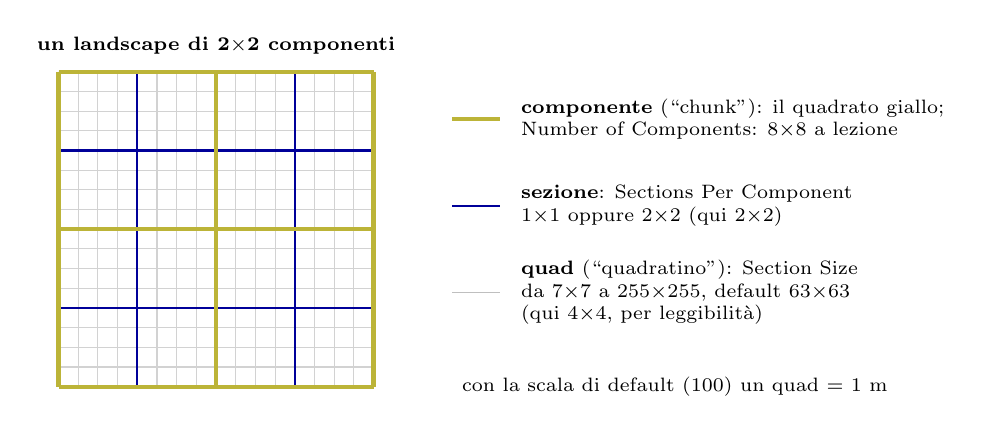
\begin{tikzpicture}[font=\footnotesize, x=1cm, y=1cm]
  % landscape 2x2 componenti, ognuno 2x2 sezioni, sezioni 4x4 quad (schematico)
  \begin{scope}
    \draw[gray!35, step=0.25] (0,0) grid (4,4);
    \draw[blue!60!black, thick, step=1] (0,0) grid (4,4);
    \draw[yellow!70!black, ultra thick, step=2] (0,0) grid (4,4);
    \node[anchor=south, font=\scriptsize\bfseries] at (2,4.1) {un landscape di 2$\times$2 componenti};
  \end{scope}
  % legenda
  \begin{scope}[xshift=5cm]
    \draw[yellow!70!black, ultra thick] (0,3.4) -- (0.6,3.4);
    \node[anchor=west, align=left, font=\scriptsize] at (0.75,3.4) {\textbf{componente} (``chunk''): il quadrato giallo;\\Number of Components: 8$\times$8 a lezione};
    \draw[blue!60!black, thick] (0,2.3) -- (0.6,2.3);
    \node[anchor=west, align=left, font=\scriptsize] at (0.75,2.3) {\textbf{sezione}: Sections Per Component\\1$\times$1 oppure 2$\times$2 (qui 2$\times$2)};
    \draw[gray!50] (0,1.2) -- (0.6,1.2);
    \node[anchor=west, align=left, font=\scriptsize] at (0.75,1.2) {\textbf{quad} (``quadratino''): Section Size\\da 7$\times$7 a 255$\times$255, default 63$\times$63\\(qui 4$\times$4, per leggibilità)};
    \node[anchor=west, align=left, font=\scriptsize] at (0,0.0) {con la scala di default (100) un quad = 1 m};
  \end{scope}
\end{tikzpicture}
\caption{La struttura di un landscape. I componenti (i \emph{chunk} gialli della preview)
sono le unità che il motore gestisce separatamente; ogni componente è diviso in una o
quattro sezioni; ogni sezione è una griglia di quad. Più quad significano curve più
morbide e più peso. Schema con valori ridotti per leggibilità.}
\label{ue14:fig:struttura}
\end{figure}

\begin{table}[htbp]
\centering
\small
\begin{tabular}{@{}p{4.2cm}p{3.0cm}p{6.8cm}@{}}
\toprule
\textbf{Parametro} & \textbf{A lezione} & \textbf{Che cosa decide} \\
\midrule
Section Size & 63$\times$63 (default); provati 31$\times$31 e 7$\times$7 & quanti quad ha
ogni sezione: più quad, terreno più morbido e più pesante \\
Sections Per Component & 2$\times$2, poi 1$\times$1 & in quante sezioni è diviso ogni
componente \\
Number of Components & 8$\times$8 & quanti componenti sulle X e sulle Y (landscape lungo,
largo, quadrato) \\
Overall Resolution & ricalcolata & il numero totale di vertici per lato (deriva dai valori
sopra) \\
Location, Rotation, Scale & invariati & la posizione e la dimensione del landscape; la scala
cambia la dimensione dei quad \\
Material & rimandato & il materiale con cui il landscape nasce \\
Fill World & non usato & crea un landscape grande quanto il mondo \\
Edit Layers & visti nella Manage & i livelli di modifica sovrapposti, bloccabili \\
\bottomrule
\end{tabular}
\caption{I parametri di creazione del landscape visti a lezione.}
\label{ue14:tab:creazione}
\end{table}

\paragraph{Approfondimento: i numeri del landscape di default.} Un quad, con la scala di
default (100 su X e Y), misura un metro: è comodo, perché la griglia del terreno coincide
con quella del pavimento della gym. La \emph{Overall Resolution} è il numero di vertici per
lato: con sezioni di 63 quad, una sezione per componente e 8 componenti per lato si hanno
$8 \times 63 + 1 = 505$ vertici, cioè un landscape di 504 metri per lato; con 2$\times$2
sezioni per componente il conto raddoppia ($8 \times 126 + 1 = 1009$). Le dimensioni
ammesse sono quelle della forma $2^n-1$ (7, 15, 31, 63, 127, 255) perché ogni livello di
LOD dimezza i quad di una sezione. Il componente è l'unità che il motore disegna, scarta e
semplifica: componenti più grandi significano meno oggetti da gestire ma un controllo più
grossolano. Epic consiglia di non esagerare con il numero di componenti (qualche migliaio
al massimo) e di scegliere le dimensioni fra quelle raccomandate nella documentazione. I
\emph{layer} della scheda Manage sono gli \textbf{Edit Layers}, attivi di default in
Unreal Engine~5: ogni layer conserva le proprie modifiche di scultura e di pittura, si può
bloccare, nascondere o cancellare senza toccare gli altri, come in un programma di grafica.
Funzionamento generale dell'engine.

% ---------------------------------------------------------------------
\section{Il pennello: falloff, strength, Alpha e Pattern}
\label{ue14:sec:pennello}

Lo strumento con cui si modifica il landscape ``è un cerchio, un pennello''. Cliccando, il
terreno si alza nel punto evidenziato: ``perché si alza? Perché siamo su \textbf{Sculpt} come
tool''. Prima degli strumenti, però, il docente spiega il pennello, che ``lascia anche
questa specie di immagine residua quando passa'' e ha una serie di parametri comuni a quasi
tutti gli strumenti (tabella~\ref{ue14:tab:pennello}).

\paragraph{Size, Falloff e Strength.}
\begin{itemize}
  \item la \textbf{grandezza} del pennello (\emph{Brush Size}), ``quindi effettivamente quanto è
        largo'';
  \item il \textbf{falloff}: ``è la distanza che c'è fra il primo cerchio e il secondo
        cerchio''. Il pennello ha due cerchi concentrici: dentro il primo l'effetto è pieno,
        fra il primo e il secondo sfuma. Con falloff \textbf{0} ``è tutto pieno'', e quando si
        alza qualcosa ``si alza tutto in blocco''; con falloff \textbf{1} ``si alza solo la
        punta e il resto è tutto quanto ammorbidito, è tutta sfumatura'';
  \item la \textbf{strength} (\emph{Tool Strength}), ``la forza del tool'': a 0,1 l'effetto si
        applica lentamente, a 1 molto più in fretta. ``È quanto forte viene applicato lo
        strumento.''
\end{itemize}

\paragraph{I quadratini e lo stretch del materiale.} ``Cosa stiamo vedendo con questi
quadratini a terra?'' La griglia disegnata sul landscape mostra ``il modo in cui sono
strutturati i poligoni'' e quindi, ``di conseguenza, in che modo verrà \textbf{stretchato il
materiale} quando ce l'andiamo a mettere sopra''. Il docente confronta tre zone
(figura~\ref{ue14:fig:stretch}): in piano ``il massimo della fedeltà, della risoluzione''; su
una salita morbida un materiale ``stretchato mediamente, ma rimane compatto''; su una parete
alzata con falloff zero un materiale che ``esplode'', perché il terreno non sale ``dritto per
dritto verticale'': c'è un quad che viene tirato in verticale ``per far sì che un lato sia
sul livello superiore, l'altro lato sul livello inferiore'', e lì il materiale ``sarà tutto
rovinato''.

\paragraph{Le forme del falloff.} Il \emph{Brush Falloff} ha quattro forme
(figura~\ref{ue14:fig:falloff}):
\begin{itemize}
  \item \textbf{Smooth}: ``il fall off è morbido'';
  \item \textbf{Linear} (``sharp linear''): ``non è morbido, ma è lineare, è geometrico'', una
        linea ``che dritta per dritta parte dalla base e arriva verso l'alto'';
  \item \textbf{Spherical}: ``un effetto più bombato'', ``una sorta di collinetta'' che poi
        ``spiove verso il basso'';
  \item \textbf{Tip}, ``il fall off convesso'', l'opposto dello spherical: la base è morbida e
        poi diventa lineare, con un effetto che ricorda ``le montagne dell'isola di Drum'' di
        \emph{One Piece} (``Drummond Island'' nella trascrizione: sono i \emph{Drum
        Rockies}, montagne a colonna).
\end{itemize}
``A seconda della situazione utilizzerete lo strumento più adatto'': linee morbide con lo
spherical, forme più aguzze con il tip.

\paragraph{I Brush Type.} ``Di base, il brush è un semplice \textbf{cerchio}''
(\emph{Circle}). Ma ci sono altri tipi:
\begin{itemize}
  \item l'\textbf{Alpha}: ``ora il nostro pennello non è più un cerchio, è una
        \textbf{texture}''. Si sceglie la texture dalla lista e ``funziona esattamente come
        avevamo fatto per i materiali: ci sono degli 0 e degli 1'': il pennello alza i bianchi
        e lascia a terra i neri. Con una texture di prova fatta di due quadrati bianchi e due
        neri si vede bene; il pennello \textbf{ruota} seguendo il movimento perché è attivo
        l'\emph{Auto Rotate}, che si può disattivare. L'uso tipico è con le texture di
        \textbf{noise}, che creano ``disturbo'': troppo, se esagerato, ma ``può esservi utile
        per andare a creare un effetto montagnoso, zigrinato, che dalla distanza può essere
        piacevole alla vista''. Qui si possono cambiare solo la grandezza e poco altro;
  \item il \textbf{canale} della texture (\emph{Texture Channel}), disponibile sia nell'Alpha
        sia nel Pattern. Il docente ripassa i canali, visti ``alla prima lezione che avevo
        fatto'': una texture ha i canali \textbf{RGB}, e i grafici li usano ``per mettere più di
        un'informazione all'interno della stessa texture'', come nelle mappe \textbf{ORM}
        (\emph{ambient occlusion} nel rosso, \emph{roughness} nel verde, \emph{metallic} nel
        blu). Il pennello può usare solo il rosso, solo il verde o solo il blu; con il noise
        ``saranno tutte uguali'';
  \item il \textbf{Pattern}: ``un portare all'estremo quello che faceva l'alfa''. La texture
        non è più ``messa su un quadrato'' ma proiettata sotto un pennello circolare, ``una
        fusione delle due precedenti'', e si può modificare: la \textbf{scala} (più piccola,
        ``molta più differenza nella costruzione''), la \textbf{rotazione}, le \textbf{U} e le
        \textbf{V}, ``quindi il \emph{panning}'', cioè lo scorrimento della texture.
        L'esempio: ``la faccia di Marte'', la collina che sembra un volto: con una texture a
        forma di faccia ``sembra che il terreno sia costruito in forma di faccia'';
  \item il \textbf{Component}, ``che io non ho mai usato, per essere onesto'': lavora
        direttamente sui componenti, per esempio per alzare un singolo chunk. Utile per
        dividere il landscape in due zone, ``una zona superiore e una zona inferiore'', che il
        giocatore dovrà collegare ``facendo X cose''.
\end{itemize}

\begin{figure}[htbp]
\centering
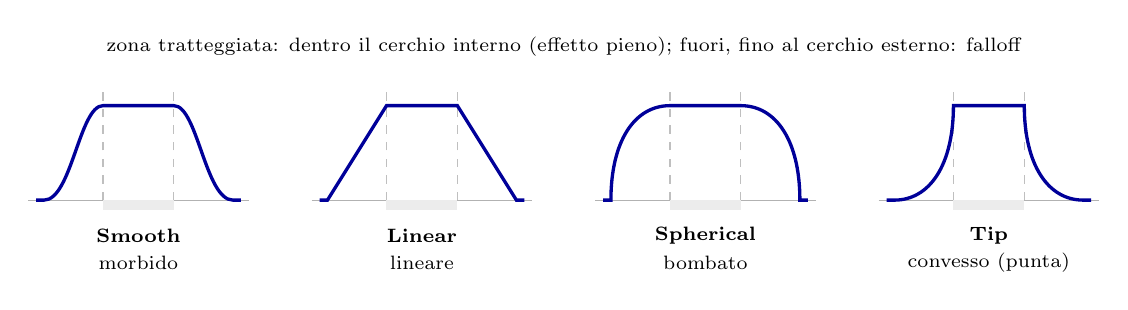
\begin{tikzpicture}[font=\footnotesize, x=1cm, y=1cm]
  \foreach \i/\name/\desc in {0/Smooth/morbido, 1/Linear/lineare, 2/Spherical/bombato, 3/Tip/convesso (punta)} {
    \begin{scope}[xshift=\i*3.6cm]
      \draw[gray!60] (-1.4,0) -- (1.4,0);
      \fill[gray!15] (-0.45,-0.12) rectangle (0.45,0);
      \draw[gray!50, dashed] (-0.45,0) -- (-0.45,1.4) (0.45,0) -- (0.45,1.4);
      \node[font=\scriptsize\bfseries] at (0,-0.45) {\name};
      \node[font=\scriptsize] at (0,-0.8) {\desc};
    \end{scope}
  }
  % Smooth: cosine
  \draw[very thick, blue!60!black] (-1.3,0) -- (-1.2,0) .. controls (-0.85,0) and (-0.75,1.2) .. (-0.45,1.2) -- (0.45,1.2) .. controls (0.75,1.2) and (0.85,0) .. (1.2,0) -- (1.3,0);
  % Linear
  \begin{scope}[xshift=3.6cm]
    \draw[very thick, blue!60!black] (-1.3,0) -- (-1.2,0) -- (-0.45,1.2) -- (0.45,1.2) -- (1.2,0) -- (1.3,0);
  \end{scope}
  % Spherical
  \begin{scope}[xshift=7.2cm]
    \draw[very thick, blue!60!black] (-1.3,0) -- (-1.2,0) .. controls (-1.2,0.75) and (-0.9,1.2) .. (-0.45,1.2) -- (0.45,1.2) .. controls (0.9,1.2) and (1.2,0.75) .. (1.2,0) -- (1.3,0);
  \end{scope}
  % Tip
  \begin{scope}[xshift=10.8cm]
    \draw[very thick, blue!60!black] (-1.3,0) -- (-1.2,0) .. controls (-0.75,0) and (-0.45,0.45) .. (-0.45,1.2) -- (0.45,1.2) .. controls (0.45,0.45) and (0.75,0) .. (1.2,0) -- (1.3,0);
  \end{scope}
  \node[font=\scriptsize, align=center] at (5.4,1.95) {zona tratteggiata: dentro il cerchio interno (effetto pieno); fuori, fino al cerchio esterno: falloff};
\end{tikzpicture}
\caption{Le quattro forme del \emph{Brush Falloff}, viste in sezione dopo aver alzato il
terreno con lo stesso pennello. Smooth sfuma in modo morbido, Linear con una rampa
dritta, Spherical con una collinetta bombata che spiove all'esterno, Tip con una base
morbida e una punta ripida. Profili schematici.}
\label{ue14:fig:falloff}
\end{figure}

\begin{figure}[htbp]
\centering
\begin{tikzpicture}[font=\footnotesize, x=1cm, y=1cm]
  % profilo del terreno con griglia di quad (vista laterale)
  \draw[gray!50] (0,0) -- (12,0);
  % piano
  \foreach \x in {0,0.5,...,3.5} {\draw[thick, green!40!black] (\x,0) -- (\x+0.5,0); \fill[green!40!black] (\x,0) circle (0.04);}
  \node[font=\scriptsize, align=center] at (2,-0.6) {piano: quad regolari\\``massima fedeltà''};
  % salita morbida
  \draw[thick, orange!80!black] (4,0) -- (4.5,0.15) -- (5,0.4) -- (5.5,0.7) -- (6,0.95) -- (6.5,1.1) -- (7,1.15);
  \foreach \p in {(4,0),(4.5,0.15),(5,0.4),(5.5,0.7),(6,0.95),(6.5,1.1),(7,1.15)} {\fill[orange!80!black] \p circle (0.04);}
  \node[font=\scriptsize, align=center] at (5.5,-0.6) {salita morbida:\\stretch medio};
  % parete
  \draw[thick, red!70!black] (7,1.15) -- (7.5,1.15) -- (8,1.15) -- (8.5,3.0) -- (9,3.0) -- (9.5,3.0);
  \foreach \p in {(7.5,1.15),(8,1.15),(8.5,3.0),(9,3.0),(9.5,3.0)} {\fill[red!70!black] \p circle (0.04);}
  \draw[red!70!black, thick] (8,1.15) -- (8.5,3.0);
  \node[font=\scriptsize, align=center, red!70!black] at (10.6,2.1) {un solo quad tirato\\in verticale: il\\materiale ``esplode''};
  \draw[-{Stealth[length=2mm]}, red!70!black] (9.7,2.1) -- (8.35,2.1);
  % texture schematica sopra la parete
  \foreach \t in {0.15,0.3,...,0.9} {\draw[red!40] ($(8,1.15)!\t!(8.5,3.0)$) -- ++(0.12,0);}
  \node[font=\scriptsize, align=center] at (8.5,-0.6) {parete con falloff 0:\\stretch estremo};
  % smooth
  \draw[-{Stealth[length=2mm]}, thick, blue!60!black] (10.4,1.0) -- (11.6,1.0);
  \node[font=\scriptsize, align=center, blue!60!black] at (11.0,0.35) {Smooth:\\quad più\\proporzionati};
\end{tikzpicture}
\caption{Lo \emph{stretch} del materiale, visto di lato. I punti sono i vertici della
griglia del landscape, a distanza fissa in pianta: in piano i quad sono regolari, su una
salita morbida si allungano un po', su una parete alzata in blocco un solo quad copre tutto
il dislivello e la texture si stira fino a diventare illeggibile. Lo strumento Smooth
riavvicina le proporzioni. Ricostruzione schematica.}
\label{ue14:fig:stretch}
\end{figure}

\begin{table}[htbp]
\centering
\small
\begin{tabular}{@{}p{3.6cm}p{10.4cm}@{}}
\toprule
\textbf{Parametro} & \textbf{Che cosa fa} \\
\midrule
Brush Size & la grandezza del pennello \\
Brush Falloff & la parte sfumata fra il cerchio interno e quello esterno: 0 tutto pieno, 1
tutto sfumato \\
Tool Strength & quanto in fretta e quanto forte si applica l'effetto (0,1 lento, 1 forte) \\
Falloff: Smooth, Linear, Spherical, Tip & la forma della sfumatura: morbida, lineare,
bombata, convessa a punta \\
Brush Type: Circle & il pennello circolare di base \\
Brush Type: Alpha & una texture come pennello: alza i bianchi, lascia i neri; Auto Rotate
lo fa ruotare con il movimento \\
Texture Channel & quale canale della texture usare (R, G o B) \\
Brush Type: Pattern & una texture proiettata sotto il pennello circolare, con scala,
rotazione e panning U/V \\
Brush Type: Component & agisce su interi componenti \\
\bottomrule
\end{tabular}
\caption{I parametri del pennello del Landscape Mode, comuni a quasi tutti gli
strumenti di scultura e di pittura.}
\label{ue14:tab:pennello}
\end{table}

\paragraph{Approfondimento: perché la parete ``esplode''.} Il landscape, essendo un
\emph{heightfield}, ha i vertici a distanza fissa in pianta: alzare un punto ne cambia solo
l'altezza, non la posizione orizzontale. Un dislivello di dieci metri fra due vertici
distanti un metro produce un quad lungo più di dieci metri e largo uno, e la texture,
mappata di default dall'alto (proiezione planare sul piano XY), vi si stira di dieci volte.
I rimedi sono tre: evitare pendenze troppo ripide (lo Smooth, che il docente chiama ``il
miglior amico dei vostri materiali''), usare nel materiale una proiezione che tenga conto
delle pareti (la proiezione \emph{triplanare} o \emph{world aligned}, che il materiale
StackOBot usa con la Absolute World Position), oppure coprire le pareti verticali con
delle mesh di roccia, come si fa quasi sempre nelle produzioni reali. Funzionamento
generale dell'engine.

% ---------------------------------------------------------------------
\section{La domanda sulle caverne}
\label{ue14:sec:caverne}

``C'è qualcosa che volevi chiedere per ora? Prima dicevi delle caverne che non si possono
fare.'' Uno studente ha provato a smanettare: è \textbf{impossibile fare dei buchi nel
landscape} con questi strumenti. Il docente conferma: ``per fare un buco avete bisogno dello
strumento \textbf{Visibility}, della \textbf{visibility mask}''. Ma la visibility mask ``si
modifica dal materiale del landscape'': bisogna aggiungere al materiale dei nodi specifici,
e solo allora si potrà avere una parte di landscape attraversabile, ``in cui possiamo andare
a costruire delle caverne''.

Lo studente pensava ad \textbf{Astroneer}, in cui scavare il terreno è la meccanica
principale. Il docente distingue due logiche: ``quando vai a creare un gioco devi far sì che
l'editor per il giocatore sia più \emph{user friendly} possibile''; ``quando stai creando un
editor, forse ti preoccupi di avere più possibilità possibili a disposizione''. Il buco ``si
può fare, non si può fare da qui''. In anteprima mostra lo strumento Visibility: il pennello
è \textbf{rosso} e cliccando non fa nulla, perché in basso Unreal avverte che il
\emph{visibility painting} è disabilitato: il componente ``non ha il nodo \textbf{Landscape
Visibility Mask} nel materiale''. Lo si vedrà a fine lezione
(sezione~\ref{ue14:sec:visibility}).

\paragraph{Approfondimento: terreni scavabili.} Giochi come Astroneer non usano un
heightfield ma un terreno \emph{volumetrico} (voxel), in cui ogni punto dello spazio sa se è
pieno o vuoto, e la superficie viene ricostruita a ogni modifica: per questo vi si possono
scavare tunnel e caverne in gioco. Il landscape di Unreal non funziona così, e una grotta
si fa nascondendo una porzione di terreno con la Visibility e costruendo l'interno con
delle mesh. Per terreni scavabili in Unreal esistono plugin di terzi basati sui voxel.
Funzionamento generale dell'engine.

% ---------------------------------------------------------------------
\section{Gli strumenti di scultura: Sculpt, Erase, Smooth, Flatten}
\label{ue14:sec:sculpt}

``Cosa fanno i nostri pennellozzi?'' ``Ognuno di voi troverà il modo con cui si trova più
comodo a fare le cose''; il docente mostra solo che cosa fa ogni strumento della scheda
\textbf{Sculpt} (tabella~\ref{ue14:tab:sculpt}).

\paragraph{Sculpt.} ``Il più semplice delle cose semplici'': scolpisce, alza il terreno. Ma,
come si è visto ``diverse volte per sbaglio'', non va solo verso l'alto: \textbf{Shift +
clic sinistro} ``scava'', e crea ``delle zone interrate'', delle depressioni.

\paragraph{Erase.} Cancella: ``elimina tutte le modifiche che abbiamo fatto, che siano verso
l'alto o verso il basso''. (Dopo la pausa il docente nota che anche l'Erase rispetta il
falloff: cancella ``in maniera sfumata'' le parti che cadono nella sfumatura.)

\paragraph{Smooth.} ``Ammorbidisce. Immaginatevelo come uno strumento che crea
sfumature.'' Se il pennello prende sia una parte alta sia una parte bassa, cliccando ``crea
una discesa più morbida'': ``fa una media, alza le parti abbassate, abbassa le parti un
pochino più alte'' e produce una \emph{slope} più leggera. ``Lo strumento Smooth è il miglior
amico dei vostri materiali'': ricordando che quanto sono stirati i quadratini ``è anche quanto
saranno stretchati i materiali'', uno smoothing li rende ``sempre più proporzionati''. Con un
pennello più grande della cima, però, ``lui abbassa proprio tutto''; per i ``lavori di fino''
si rimpicciolisce il pennello e si fanno piccole modifiche ``che non vanno a sbragare
completamente tutta la parete''. Anche qui ci sono falloff, tipi di pennello e strength, e
un parametro in più per la \textbf{precisione} dello smoothing (il \emph{Detail Smooth}):
``più grande è questo valore, più dettagli vengono rimossi'', più piccolo, ``meno dettagli
vengono rimossi''. I ``dettagli'' sono ``tutti questi su e giù'': con un valore alto e un
pennello grande ``lui pialla tutto'', con un valore piccolo i cambiamenti sono ``molto
morbidi'' e ``molto precisi''; ``a zero chiaramente non farà mai nulla''.

\paragraph{Flatten.} ``Il mio strumento preferito.'' Il docente si costruisce ``un piccolo
parco giochi'' di colline per gli esempi. Il \textbf{Flatten} ``ci permette di selezionare un
punto e appiattire tutto quanto a quell'altezza'': si clicca dove c'è la croce e tutto ciò
che passa sotto il pennello viene portato a quell'altezza, sia in basso sia sulla vetta.
Serve a una ``terraformazione un po' più controllata'':
\begin{itemize}
  \item \textbf{plateau}, altopiani: il ``lenzuolo'' tirato su si interrompe al bordo,
        ``non riscende giù'';
  \item \textbf{scaloni}, cliccando su punti diversi di una slope: ``scalone, altro scalone,
        altro scalone'', ``delle formazioni un po' più sensate, un po' più normali'', da
        ammorbidire poi con lo Smooth. Per esempio ``le cascatine fatte a livelli'' o ``le
        \textbf{risaie}'', con parti piatte e parti rialzate;
  \item un \textbf{canyon} dentro una parte rialzata: un fondo appiattito e i lati rimasti
        alti.
\end{itemize}

\paragraph{Le modalità del Flatten.} ``È abbastanza brutale come strumento, perché prende e
appiattisce tutto'': si rischia di appiattire le cose sbagliate. Per questo c'è la
\textbf{Flatten Mode} (figura~\ref{ue14:fig:flatten}):
\begin{itemize}
  \item \textbf{Both} (default): ``alza i piani che stanno più in basso e abbassa i piani che
        stanno più in alto'';
  \item \textbf{Raise}: alza tutti i punti fino all'altezza scelta, ``però non abbassa''.
        Esempio: un rilievo che fa da \textbf{bordo della mappa} resta intatto, e si alza
        solo ciò che c'è sotto;
  \item \textbf{Lower}: abbassa ``tutto quello che c'è da abbassare, ma non alza'': ``se c'è
        una grotta o un canyon che deve rimanere giù, non lo tira più su''.
\end{itemize}
``Principalmente questi sono i due che vorrete utilizzare, perché sono quelli che vi danno
un po' più di controllo.'' Di un'altra opzione il docente legge a fatica il nome (``height
intervals'', ``specification at intervals''): ``questo è uno che effettivamente non ho mai
utilizzato''. Si tratta, con ogni probabilità, della modalità \textbf{Terrace} (si veda
l'approfondimento).

\paragraph{Use Slope Flatten.} Con la casella \textbf{Use Slope Flatten}, invece di
appiattire in orizzontale ``andate a continuare il piano diagonale preso originariamente'':
cliccando su un pendio, lo strumento prolunga quella pendenza, ``anche scavando verso il
basso''. Serve per ``quei pianori, quegli spiazzi montani'' che sono ``uno spaccato dritto per
dritto, che però va in diagonale''. Ultimo uso, personale: ``a volte il Flatten tendo a
utilizzarlo tipo \textbf{gomma}'': si punta sul livello base del landscape e si appiattisce.

``Abbiamo visto scolpire, tirare su, tirare giù, ammorbidire, cancellare e appiattire.''

\begin{figure}[htbp]
\centering
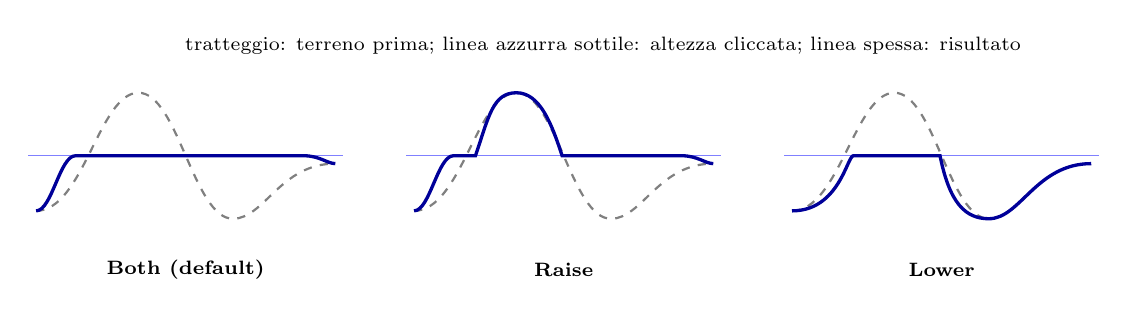
\begin{tikzpicture}[font=\footnotesize, x=1cm, y=1cm]
  \foreach \i/\name in {0/Both (default), 1/Raise, 2/Lower} {
    \begin{scope}[xshift=\i*4.8cm]
      % profilo originale
      \draw[gray, dashed, thick] (0,0.3) .. controls (0.6,0.3) and (0.8,1.8) .. (1.3,1.8) .. controls (1.8,1.8) and (2.0,0.2) .. (2.5,0.2) .. controls (2.9,0.2) and (3.1,0.9) .. (3.8,0.9);
      \draw[blue!50, thin] (-0.1,1.0) -- (3.9,1.0);
      \node[font=\scriptsize, blue!60!black, anchor=west] at (3.9,1.0) {};
      \node[font=\scriptsize\bfseries] at (1.9,-0.45) {\name};
    \end{scope}
  }
  % Both: tutto a 1.0
  \draw[very thick, blue!60!black] (0,0.3) .. controls (0.2,0.3) and (0.3,1.0) .. (0.5,1.0) -- (3.4,1.0) .. controls (3.6,1.0) and (3.7,0.9) .. (3.8,0.9);
  % Raise: alza le valli, non abbassa la cima
  \begin{scope}[xshift=4.8cm]
    \draw[very thick, blue!60!black] (0,0.3) .. controls (0.2,0.3) and (0.3,1.0) .. (0.5,1.0) -- (0.78,1.0) .. controls (0.95,1.5) and (1.0,1.8) .. (1.3,1.8) .. controls (1.6,1.8) and (1.75,1.4) .. (1.88,1.0) -- (3.4,1.0) .. controls (3.6,1.0) and (3.7,0.9) .. (3.8,0.9);
  \end{scope}
  % Lower: abbassa la cima, non alza le valli
  \begin{scope}[xshift=9.6cm]
    \draw[very thick, blue!60!black] (0,0.3) .. controls (0.6,0.3) and (0.7,1.0) .. (0.78,1.0) -- (1.88,1.0) .. controls (2.0,0.4) and (2.2,0.2) .. (2.5,0.2) .. controls (2.9,0.2) and (3.1,0.9) .. (3.8,0.9);
  \end{scope}
  \node[font=\scriptsize, align=center] at (7.2,2.4) {tratteggio: terreno prima; linea azzurra sottile: altezza cliccata; linea spessa: risultato};
\end{tikzpicture}
\caption{Le tre modalità principali del Flatten, in sezione. Both porta tutto all'altezza
cliccata; Raise alza solo ciò che sta sotto e lascia la cima (per esempio il bordo della
mappa); Lower abbassa solo ciò che sta sopra e lascia le valli (per esempio un canyon).
Profili schematici.}
\label{ue14:fig:flatten}
\end{figure}

\paragraph{Approfondimento: Terrace e gli altri parametri del Flatten.} Nella versione di
Unreal Engine~5 il Flatten ha quattro modalità: oltre a Both, Raise e Lower, la modalità
\textbf{Terrace}, che appiattisce il terreno a \emph{intervalli} di altezza regolari
(\emph{Terrace Interval}), con una sfumatura fra un gradino e l'altro (\emph{Terrace
Smooth}): è lo strumento giusto per le risaie e le cascate a livelli che il docente
costruisce a mano cliccando su più punti. Altri parametri utili: \emph{Pick Value Per
Apply}, che ricampiona l'altezza a ogni pennellata invece di tenere quella del primo clic;
\emph{Flatten Target}, che permette di scrivere a mano l'altezza a cui appiattire (comodo
per avere esattamente le misure della gym, per esempio un plateau a 1,40 m sopra un
altro); e \emph{Show Preview Grid}, che mostra il piano di destinazione. Funzionamento
generale dell'engine; la lezione non li tocca.

% ---------------------------------------------------------------------
\section{Ramp e i LOD}
\label{ue14:sec:ramp}

``Adesso vediamo uno strumento che funziona in maniera un po' diversa. Non è più un
pennello, ma dei clic'': lo strumento \textbf{Ramp}. Si clicca su due punti, li si sposta
come si vuole, e quando si è contenti si preme \textbf{Add Ramp}: Unreal aggiunge ``un
collegamento di landscape da punto A a punto B''. Il docente chiede alla classe che cosa
succederà con due punti sul fondo di due valli separate da una collina: ``ti farà un canyon
lì in mezzo'' (la rampa porta il terreno ``sempre da punto A a punto B'', anche scavando).

\paragraph{Gli usi.}
\begin{itemize}
  \item una \textbf{rampa} per salire su un punto sopraelevato (``sarà un modo molto brutto,
        però va'');
  \item le rampe di un gioco di \textbf{macchine} o di \textbf{skateboard};
  \item ``una \textbf{diga} in un crepaccio'', un collegamento pieno da una parte all'altra.
\end{itemize}
Un \textbf{ponte sospeso}, invece, no. Si potrebbe pensare di fare la diga e poi bucarla
sotto con la Visibility, ``tuttavia ci sarebbe un problema'': la parte sotto non
collegherebbe più le due metà, ``perché il landscape \textbf{non può essere sovrapposto}'',
``non può esserci una parte qui e una parte sotto''. ``Se volete fare un ponte sospeso,
fatelo con le \textbf{mesh}: prendete una mesh, ingranditela e mettetela sopra un crepaccio.
Non fatelo con il landscape.''

\paragraph{Larghezza e falloff.} La rampa ha la sua \textbf{larghezza} (\emph{Ramp Width}),
``se un ponticello, se una grossa salita'', e il suo \textbf{falloff} (\emph{Side Falloff}):
a zero non c'è sfumatura e i lati vengono stirati ``a blocco''; tutto sfumatura, e il
terreno attorno si raccorda morbido. Ma se si ``tira la corda'', con molta sfumatura e una
rampa molto stretta, ``vi si spacca un po' il landscape'': ``questa cosa è molto rotta, e
dalla distanza sarà tremenda'', ``perché i \textbf{LOD} vanno a semplificare il landscape''.

\paragraph{I LOD.} ``Sapete che cos'è un LOD?'' \textbf{LOD} sta per \emph{Level of Detail}.
Un grafico crea una mesh, poniamo da 10.000 poligoni; questa mesh deve avere ``altre
versioni di sé più grezze'', da 5.000, da 2.000 poligoni, perché l'engine, ``e non solo in
automatico'', aggiorna il numero di poligoni ``a seconda della distanza da cui lo vedi''.
L'esempio della statua: da vicino deve essere ``super bellissima'', ma da lontano ``non serve
che abbia ancora 500.000 poligoni'', perché l'occhio non vedrà il dettaglio, e ridurli
alleggerisce le prestazioni. Le distanze si possono impostare (``a 10 metri un tot, a 20
metri un altro tot, a 40 metri un altro tot''), da un Blueprint o dalla mesh stessa. Il
landscape funziona allo stesso modo: dalla distanza i suoi poligoni vengono semplificati.
Una massa grande non ne soffre, ``perché ci sono molti poligoni''; una rampa sottilissima,
``costituita di troppi pochi poligoni, viene distrutta dai LOD''. ``Quindi evitate di fare
delle robe in questo modo.''

\paragraph{Lo sfogo sui Pokémon.} L'esempio, dichiaratamente polemico: i recenti Pokémon
open world, \emph{Scarlatto e Violetto} e \emph{Leggende Pokémon: Arceus}. ``Potete vedere
attivamente la terra che si muove, come se fosse animata'': ``sono semplicemente i LOD che si
attivano troppo presto'', il landscape ``viene semplificato con troppo anticipo''. Il
motivo, secondo il docente, è l'ottimizzazione: se in una visione ampia si vedesse tutto
con tutti i poligoni ``esploderebbe la console''. ``Non è che sono brutte, ma è che sono
troppo ottimizzate, e la troppa ottimizzazione le rende orribili''; e sono così ottimizzate
``perché il gioco è programmato in maniera talmente stupida da essere pesante''. ``Scusate
questo piccolo sfogo contro Game Freak.'' (È un giudizio personale del docente, non
un'analisi tecnica verificata; il fenomeno del terreno che ``si muove'' quando cambia il LOD,
il \emph{LOD popping}, è comunque reale e ben noto.)

\paragraph{La regola.} ``Diamo sempre un po' di spazio al landscape'': niente forme troppo
sottili. ``Questo è anche il motivo per cui vorremmo evitare dei landscape troppo piccoli'':
un landscape 7x7 ``capita molto spesso che si spacchi in questo modo, perché ha pochi
poligoni a disposizione''. Il docente rifà ``una rampina decente''.

\paragraph{Approfondimento: i LOD del landscape.} Il landscape non ha LOD costruiti a mano
come una static mesh: li calcola da solo, dimezzando a ogni livello i quad di ogni sezione
(per questo le Section Size sono della forma $2^n-1$). La transizione è regolata da
parametri dell'actor Landscape (in Unreal Engine~5 \emph{LOD 0 Screen Size}, \emph{LOD 0
Distribution Setting} e \emph{LOD Distribution Setting}, più eventuali \emph{LOD Group}),
che decidono a quale dimensione sullo schermo un componente passa al livello successivo.
Aumentarli rende il terreno lontano più fedele e più costoso. Le forme più sottili di una
sezione, come la rampa stretta del docente, sono le prime a sparire perché nel livello
semplificato non ci sono più vertici abbastanza vicini per descriverle. Il capitolo 12 di
Romero e Sewell, sulla pubblicazione, ricorda che fra le impostazioni di scalabilità del
gioco c'è anche la qualità del \emph{foliage}, e che se le prestazioni calano solo in certe
zone del livello conviene ``ridurre la densità degli oggetti'' o la qualità di un modello:
il compromesso fra dettaglio e prestazioni di cui parla il docente. Per la parte sui
parametri del landscape, funzionamento generale dell'engine.

% ---------------------------------------------------------------------
\section{Erosion, Hydro, Noise, Mirror e Copy/Paste}
\label{ue14:sec:altristrumenti}

\paragraph{Erosion e Hydro.} ``Sono due strumenti con cui io faccio un po' a botte'' (``a
volte'' nella trascrizione, ma il seguito chiarisce il senso): il
docente spiega a che cosa servirebbero e perché non gli piacciono. L'idea è ``simulare
delle deformazioni, del \emph{displacement}''. L'\textbf{Erosion} è lo strumento con cui
``andrei a dettagliare una parete montuosa'': ``è un po' il contrario dello smooth'', crea
nel pennello parti rialzate e parti abbassate. (Qui la trascrizione si interrompe in una
frase ripetuta; riprende con la domanda di uno studente.)
\begin{itemize}
  \item il \textbf{Threshold} ``va a definire quanta differenza fra punto A e punto B deve
        esserci per andare a fare erosione'': con un valore alto l'erosione si applica solo
        dove il dislivello è grande; abbassandolo (``tipo 17'') si erode ``molto di più, in
        molti punti diversi'', perché basta una differenza minore;
  \item \textbf{Noise Mode} e \textbf{Noise Scale} aggiungono un rumore preimpostato, e come
        nel Flatten si sceglie se deve alzare e abbassare, solo alzare o solo abbassare.
\end{itemize}
L'\textbf{Hydro} (\emph{Hydro Erosion}) ``funziona più o meno nello stesso modo'' e
vorrebbe creare un \emph{displacement} ``stile fondali marini'' o ``erosione dell'acqua''. Il
problema è che ``abbiamo un po' poco controllo'': ``io non sono mai riuscito a farlo
funzionare bene, proprio non mi trovo''.

\paragraph{Noise.} ``Preferisco piuttosto utilizzare il \textbf{Noise}'', che ``fa rumore'' e
permette di scegliere se aggiunge, se toglie o se fa entrambe le cose. Con un pennello
grande e la scala del noise ridotta, ``vi va a fare una deformazione un po' più subdola'':
``non prende e spacca, ma fa dei leggeri movimenti di alzare e abbassare'', il risultato
``che al mio occhio è sempre il più piacevole''. In modalità solo-aggiunta il Noise alza,
``però non come lo Sculpt'' (aggiunge rumore, non una collina); lo stesso vale per la
sottrazione.

\paragraph{Gli strumenti saltati.} ``Facciamo al volissimo le ultime cose'':
\begin{itemize}
  \item il \textbf{Retopologize} ``non ci interessa'';
  \item la \textbf{Visibility}, già vista, si riprende più avanti;
  \item il \textbf{Blueprint Brush}, ``qualcosa che onestamente non ho mai utilizzato'':
        ``presumo sia un brush che può essere programmato'' per fare cose specifiche. ``Non
        l'ho mai trovato necessario.''
\end{itemize}

\paragraph{Mirror.} Il \textbf{Mirror} serve ``nel momento in cui avete degli ambienti molto
grandi che volete copiare, che volete specchiare o che volete ruotare''. Compare un
\textbf{piano}: premendo \textbf{Apply}, tutto ciò che sta da un lato viene copiato
sull'altro, ``appiattendo'' quello che c'era. Il piano si sposta avanti e indietro, e
soprattutto dall'\textbf{Operation} si sceglie il tipo di operazione:
\begin{itemize}
  \item \textbf{-X to +X}: copia il lato sinistro sul destro; \textbf{+X to -X} il contrario;
        lo stesso per \textbf{-Y to +Y} e \textbf{+Y to -Y}. Con una forma qualsiasi si ottiene
        ``una macchia di Rorschach'';
  \item le varianti \textbf{Rotate} (per esempio \emph{Rotate -X to +X}): stessa direzione del
        piano, ``ma operazione diversa'': invece di specchiare, ruota, ``come se prendesse
        questa parte del landscape e la ruotasse nell'altra direzione''. Il risultato è
        uguale, ``ma ruotato''.
\end{itemize}

\paragraph{Copy/Paste.} ``Il copia e incolla, la cosa più semplice del mondo.'' Prima si
seleziona una parte di landscape con lo strumento \textbf{Region Select} (``Select''),
dipingendo la zona con il pennello; per togliere la selezione serve \textbf{Clear Region
Selection}, ``perché se andate da altre parti questo vi rimane sempre selezionato''. Poi,
nello strumento \textbf{Copy/Paste}, \textbf{Ctrl+C} copia la zona in un riquadro (il
\emph{gizmo}) che si può spostare, ruotare e scalare dove si vuole, e \textbf{Ctrl+V} la
incolla, ``modificata, ruotata e anche scalata''. Ci sono comandi per adattare il riquadro
alla selezione e per ripulirlo. La \textbf{Paste Mode} ripete la logica del Flatten:
\begin{itemize}
  \item \textbf{Both}: tutto il riquadro viene portato al livello copiato, la zona di
        destinazione viene abbassata a livello base e la parte copiata rialzata;
  \item \textbf{Raise}: alza soltanto ``le parti che erano più basse'' e non abbassa le altre:
        di una collina copiata sopra un'altra resta solo ``la punta'';
  \item \textbf{Lower}: l'opposto.
\end{itemize}
``Abbiamo effettivamente un po' tutte le cose viste.'' Nessuna domanda: pausa, ``ci becchiamo
alle 55 con il Paint, e quindi i materiali del landscape''.

\begin{table}[htbp]
\centering
\small
\begin{tabular}{@{}p{3.0cm}p{11.0cm}@{}}
\toprule
\textbf{Strumento (Sculpt)} & \textbf{Che cosa fa, e come lo usa il docente} \\
\midrule
Sculpt & alza il terreno; Shift + clic scava \\
Erase & cancella le modifiche (rispetta il falloff) \\
Smooth & fa una media delle altezze; Detail Smooth decide quanto dettaglio togliere; ``il
miglior amico dei materiali'' \\
Flatten & appiattisce all'altezza cliccata; Flatten Mode Both, Raise, Lower (e Terrace);
Use Slope Flatten prolunga il pendio; usato anche come ``gomma'' \\
Ramp & crea una rampa fra due punti (Add Ramp), con Ramp Width e Side Falloff; non per i
ponti sospesi \\
Erosion & dettaglia le pareti erodendo dove il dislivello supera il Threshold; Noise Mode e
Noise Scale; ``poco controllo'' \\
Hydro (Hydro Erosion) & erosione ``ad acqua''; il docente non lo usa \\
Noise & aggiunge o toglie rumore; con scala piccola, deformazioni ``subdole'' \\
Retopologize & non visto (``non ci interessa'') \\
Visibility & nasconde porzioni di terreno; richiede la Landscape Visibility Mask nel
materiale \\
Blueprint Brush & pennelli programmabili; mai usato dal docente \\
Mirror & specchia (-X to +X, \dots) o ruota (Rotate \dots) metà del landscape; Apply \\
Region Select & seleziona una zona col pennello; Clear Region Selection \\
Copy/Paste & Ctrl+C e Ctrl+V di una zona, con gizmo spostabile, ruotabile, scalabile;
Paste Mode Both, Raise, Lower \\
\bottomrule
\end{tabular}
\caption{Gli strumenti della scheda Sculpt del Landscape Mode, nell'ordine della lezione.}
\label{ue14:tab:sculpt}
\end{table}

\paragraph{Approfondimento: il terreno come spazio di gioco.} Gli strumenti di scultura
sono tecnici, ma le forme che producono sono categorie di level design. Totten, nel
capitolo 3, osserva che in un open world fatto di paesaggi aperti, come \emph{Skyrim}, i
percorsi fra città e dungeon ``sono molto meno diretti'' e spesso ``campi aperti'': il
giocatore traccia da sé le scorciatoie fra i landmark, ma ``rischia di perdersi'', e i
designer usano ``elementi geografici sottili come sentieri sterrati, cartelli o fiumi'' per
suggerire i percorsi. E aggiunge proprio a proposito degli ``editor di terreno integrati
nell'engine'': tenere a mente queste linee guida serve a creare mondi ``non solo
esteticamente attraenti, ma anche utilizzabili''. Il canyon del Flatten, la diga della Ramp
e il bordo di mappa preservato dal Raise sono, in questi termini, un percorso, un
collegamento e un \emph{edge}; il plateau è un'area in cui il giocatore guarda lontano (il
\emph{prospect space} dello stesso capitolo). Le misure, infine, vengono dalla gym: un
canyon che deve essere invalicabile avrà pareti oltre il Walkable Floor Angle del
personaggio, un plateau raggiungibile con un salto starà sotto l'altezza comoda misurata.

% ---------------------------------------------------------------------
\section{La pausa e la domanda su The Sims}
\label{ue14:sec:pausa}

Alla ripresa (``Guido c'è, Federico c'è, Giulia c'è'') il docente chiede se sia tutto
chiaro: ``è abbastanza semplice, è più una questione di prenderci la mano''. Consiglia di
usare il landscape ``fra questa lezione e la prossima'' per familiarizzare e trovare il
proprio modo di lavorare: ``magari siete dei pazzi completi e lavorate utilizzando soltanto
lo Sculpt, ma siete fortissimi. Io vi dico quali sono i tool, poi voi trovate il vostro
modo di lavoro''.

\paragraph{The Sims.} Uno studente chiede se il terreno della serie \textbf{The Sims}, ``soprattutto
del 2'', sia fatto allo stesso modo. Il docente non lo sa: ``non so con cosa è stato fatto''.
Dopo un rapido controllo: ``a quanto risulta, ogni The Sims ha usato un \textbf{engine custom}''.
È ``plausibile'' che funzioni in modo simile, e che ci sia stata ``una \emph{cross
contamination}, delle influenze da entrambe le parti'': magari anche Unreal si è ispirato a
come ``diversi tycoon o diversi simulatori'' gestivano la terraformazione, perché ``quel tipo
di modifica spaziale è molto comodo farla con un pennello''. ``Non ti so dire di più'':
l'ultima volta che ha giocato a The Sims ``probabilmente era vent'anni fa''. Lo invita a fare
una ricerca e a riferire la volta successiva. (Nello scambio, alla domanda ``quando è uscito
The Sims 2?'', la risposta è ``nel 2000'': in realtà nel 2000 è uscito il primo
\emph{The Sims}; \emph{The Sims 2} è del 2004.)

% ---------------------------------------------------------------------
\section{Il Paint e il materiale del landscape di StackOBot}
\label{ue14:sec:paint}

``Abbiamo visto il Manage, abbiamo visto lo Sculpt, rimane soltanto da vedere il
\textbf{Paint}.'' La scheda ha ``più o meno gli stessi strumenti che c'erano di là'':
\textbf{Paint}, \textbf{Smooth}, \textbf{Flatten} e \textbf{Noise}, con la stessa strength e
gli stessi tipi di pennello. Ma in basso Unreal avverte: \emph{non ci sono target layer
assegnati a questo landscape; usa i bottoni in alto per aggiungerne di nuovi o popolarli
dal materiale correntemente assegnato}. I bottoni sono \textbf{Create Layer} e
\textbf{Create Layers from Assigned Materials}, quest'ultimo, ``se non sbaglio, unico di
Unreal 5, sulla quarta edizione non c'è''.

\paragraph{Un materiale normale non basta.} Il landscape può \textbf{dipingere il materiale}
con il pennello, ``il materiale però deve essere fatto \emph{ad hoc}''. Prova: un nuovo
materiale con dentro ``unicamente un colore''. Messo sul landscape, il landscape lo tratta
``come un oggetto qualsiasi'': ``tutto quanto diventa disgustosamente verde'', e non c'è modo
di modificare nulla, ``perché il nostro materiale di layer non ne ha''.

\paragraph{Il ``grosso errore''.} A questo punto il docente si accorge di ``aver fatto un grosso
errore: niente di grave, semplicemente una cosa che ci farà perdere un po' di tempo'' (la
spiegherà più avanti: sono le Virtual Texture, sezione~\ref{ue14:sec:grass}).

\paragraph{Il pacchetto StackOBot.} Fra gli asset del pacchetto \textbf{StackOBot}, ``il
pacchettino con il robottino e tutte le cose'', nella cartella \emph{Environment} ci sono:
\emph{Props} e \emph{Modular} (mesh da vedere alla fine della lezione ``o all'inizio della
prossima''), \emph{Materials}, \emph{Foliage} (per il Foliage Mode) e \textbf{Landscape}, con
``tutto quello che riguarda il landscape'': delle texture ``che non sappiamo bene cosa
fanno'', una mesh che per ora non serve, dei materiali, fra cui \textbf{M\_Landscape}, e dei
\textbf{Landscape Layers} ``che non sappiamo bene cosa fanno'' e che si rivedranno più
tardi.

\paragraph{Il nero.} Si assegna M\_Landscape al landscape (nel campo \emph{Landscape
Material} dei Details): ``va tutto \textbf{nero}''. Anche un materiale pensato per il
landscape, appena assegnato, ``non ci dà subito quello di cui abbiamo bisogno''; e ``il fatto
che diventi tutto nero è quello che vogliamo, per noi è positivo''. Bisogna stabilire come
funzionano i layer: visto che il materiale ``è già stato costruito per avere tanti layer
diversi'', si preme \textbf{Create Layers from Assigned Materials}. Unreal crea
\textbf{quattro layer}, e il terreno resta nero. (Resta nero perché nessun layer è ancora
stato dipinto: si veda l'approfondimento.)

\paragraph{Dentro M\_Landscape.} Il docente apre il materiale, ``molto piccolo, vero?
Molto comodo'' (ironico: il nodo principale è ridotto a un solo pin). Le parti interessanti:
\begin{itemize}
  \item quattro \textbf{material function}, \emph{MF\_Rocks}, \emph{MF\_Pebbles},
        \emph{MF\_Sand} e \emph{MF\_Grass}: ``il funzionamento dei singoli materiali, quindi
        dei singoli layer''. Si creano con tasto destro, \emph{Material Function}: sono
        ``delle piccole funzioni'', come quelle dei Blueprint, che descrivono ``come funziona
        l'erba, come funziona la ghiaia, i \emph{pebbles}'', la roccia e la sabbia;
  \item dentro ogni funzione le texture sono collegate alla \textbf{Absolute World
        Position}: ``vi ricordate i materiali \textbf{world aligned} che avevamo visto la
        volta scorsa? Questo è il modo per farli, anche per il landscape'';
  \item tutte le funzioni terminano con un nodo \textbf{Set Material Attributes}: un nodo
        ``vuoto'' in cui, aggiungendo slot all'array, si decide quale informazione passa ogni
        ingresso (Base Color, Metallic, Specular, Roughness, Normal\dots). Qui ogni funzione
        passa \textbf{Base Color}, \textbf{Roughness} e \textbf{Normal} del proprio materiale,
        presi da dei \emph{Texture Sample} (``vi ricordate, l'abbiamo fatta questa roba'');
  \item le quattro uscite entrano nel nodo che è ``alla base del funzionamento del
        materiale del landscape'': il \textbf{Landscape Layer Blend}.
\end{itemize}

\paragraph{I nodi del landscape.} Cercando \emph{landscape} nella palette dei nodi, Unreal
mostra ``tutti i nodi che sono utili per il landscape''. Oggi se ne vedono tre (più uno ``che
sta da un'altra parte'', il Landscape Grass Output): il \textbf{Landscape Layer Blend},
``il fondamentale'', il \textbf{Landscape Layer Sample} e la \textbf{Landscape Visibility
Mask}.

\paragraph{Landscape Layer Blend.} È un nodo ``vuoto'', come il Set Material Attributes, in
cui si aggiungono elementi all'array \emph{Layers}. Ogni elemento si apre con delle
freccette, e lì si scrive il \textbf{nome del layer} (per esempio \emph{Grass}).
``Scriveteli bene, perché è importante scrivere bene il nome del layer'': se non c'è il
nome, ``Unreal non lo trova, non lo rileva'', anche se ci sono collegate delle cose; e altri
nodi, come il Landscape Layer Sample, ``hanno bisogno del nome per funzionare''. Gli altri
campi dell'elemento ``sono dei parametri di preview che al momento non ci interessano''.
Usando questo nodo, gli autori del materiale hanno fatto quattro layer: \textbf{roccia},
\textbf{sassolini} (ghiaia), \textbf{sabbia} ed \textbf{erba}, tutti collegati al nodo
risultante del materiale.

\paragraph{Use Material Attributes.} Il nodo risultante è ``così piccolino'' perché nei
dettagli del materiale è spuntata la casella \textbf{Use Material Attributes}, che
``trasforma il modo in cui funziona il nodo'': invece di avere un pin per Base Color, uno per
Roughness, uno per Normal, ha un unico ingresso \emph{Material Attributes}. Senza la casella
bisognerebbe collegare il risultato su ogni parametro, cosa comoda se si vogliono
modificare le singole cose; ma poiché tutte le operazioni avvengono nelle funzioni, ``per
lui è comodo'' far passare tutto in un colpo solo.

\paragraph{Dipingere.} Che cosa permette la suddivisione in layer? ``Di avere dei layer da
poter dipingere.'' Selezionato \textbf{Rock} e passato il pennello, il terreno ``dipinge
roccia'', ``o perlomeno quello che noi abbiamo impostato come valore per il materiale della
roccia'': se non piace, la texture e le dimensioni si cambiano da dentro la sua material
function, ``tutto come abbiamo visto la volta scorsa''. Poi i \textbf{Pebbles} (``dei
sassolini, una ghiaietta''), la \textbf{Sand} e la \textbf{Grass}. Ogni volta Unreal deve
``compilare gli shader'', e ci vuole un po'.

\begin{figure}[htbp]
\centering
\begin{tikzpicture}[font=\scriptsize, x=1cm, y=1cm,
  ue14node/.style={draw, thick, rounded corners=2pt, fill=white, align=center, minimum height=0.6cm, inner sep=3pt},
  ue14fn/.style={ue14node, fill=yellow!15},
  ue14out/.style={ue14node, fill=gray!25, minimum width=2.6cm},
  ue14arr/.style={-{Stealth[length=1.6mm]}, thick}]
  \node[ue14fn] (r) at (0,3.0) {MF\_Rocks};
  \node[ue14fn] (p) at (0,2.2) {MF\_Pebbles};
  \node[ue14fn] (s) at (0,1.4) {MF\_Sand};
  \node[ue14fn] (g) at (0,0.6) {MF\_Grass};
  \node[font=\scriptsize, align=center] at (0,3.9) {material function:\\Texture Sample (World Position)\\$\rightarrow$ Set Material Attributes};
  \node[ue14node, minimum height=3.0cm, minimum width=2.8cm] (lb) at (4.2,1.8) {};
  \node[font=\scriptsize\bfseries] at (4.2,3.55) {Landscape Layer Blend};
  \foreach \n/\y in {Rock/2.6,Pebbles/2.0,Sand/1.4,Grass/0.8} {\node[font=\scriptsize, anchor=west] at (3.0,\y) {Layer \n};}
  \draw[ue14arr] (r.east) -- (3.0,2.6);
  \draw[ue14arr] (p.east) -- (3.0,2.0);
  \draw[ue14arr] (s.east) -- (3.0,1.4);
  \draw[ue14arr] (g.east) -- (3.0,0.8);
  \node[ue14out] (m) at (8.6,1.8) {M\_Landscape\\(Use Material Attributes)\\\emph{Material Attributes}};
  \draw[ue14arr] (lb.east) -- (m.west);
  % grass spawn
  \node[ue14node, fill=green!12] (ls) at (0.6,-1.2) {Landscape Layer Sample\\\emph{Parameter Name: Grass}};
  \node[ue14node] (calc) at (4.2,-1.2) {calcoli\\(GPU Grass Spawn)};
  \node[ue14out, fill=green!25] (go) at (8.6,-1.2) {Landscape Grass Output\\\emph{Grass: GT\_Grass}};
  \draw[ue14arr] (ls.east) -- (calc.west);
  \draw[ue14arr] (calc.east) -- (go.west);
  \node[ue14node, fill=blue!8] (gt) at (8.6,-2.6) {Landscape Grass Type: mesh,\\densità, scala min--max};
  \draw[ue14arr, dashed] (gt.north) -- (go.south);
  \node[font=\scriptsize, align=left, anchor=west] at (-1.4,-2.6) {i nomi \emph{Grass} devono coincidere\\esattamente (maiuscole comprese)};
\end{tikzpicture}
\caption{Lo schema del materiale M\_Landscape di StackOBot come descritto a lezione. In
alto, la parte che \emph{dipinge}: quattro material function entrano nel Landscape Layer
Blend, ognuna nel layer con il proprio nome, e il risultato va al nodo del materiale con
Use Material Attributes. In basso, la parte separata che \emph{fa spawnare} l'erba: un
Landscape Layer Sample legge dove è stato dipinto il layer Grass e, dopo alcuni calcoli,
alimenta il Landscape Grass Output, che usa un Landscape Grass Type. I nodi grigi sono
nodi finali. Ricostruzione schematica.}
\label{ue14:fig:materiale}
\end{figure}

\paragraph{Approfondimento: perché il terreno è nero, e i pesi dei layer.} Un materiale del
landscape non sceglie da solo dove mettere la roccia o l'erba: per ogni layer il landscape
memorizza una \emph{weightmap}, una mappa di pesi da 0 a 1 per ogni vertice, e il Landscape
Layer Blend mescola i layer secondo quei pesi. Appena assegnato il materiale, nessun layer
ha ancora un peso, quindi la somma è zero e il risultato è nero: per questo il docente lo
considera un buon segno. Quando si dipinge il primo layer su un componente, i pesi
cominciano a esistere; dipingere un layer riduce gli altri nello stesso punto, perché in un
layer \emph{weight-blended} la somma dei pesi resta 1. Il primo layer della lista viene
spesso usato come ``fondo'' e si può riempire tutto il terreno con il comando \emph{Fill
Layer} (tasto destro sul layer nella scheda Paint). Ogni layer in più costa: Unreal campiona
le texture di tutti i layer presenti su un componente, e per questo conviene non usarne
troppi per componente. Il pulsante \emph{Create Layers from Assigned Materials} legge i
nomi dei layer dal Landscape Layer Blend del materiale e crea i target layer
corrispondenti; se nel progetto esistono già le relative \emph{Layer Info} (come nel
pacchetto StackOBot) le collega, altrimenti vanno create. Il libro di Romero e Sewell
mostra il Material Editor e i pin Base Color, Metallic e Roughness nel capitolo 5, ma non
tratta i materiali del landscape; il resto si basa sul funzionamento generale dell'engine.

% ---------------------------------------------------------------------
\section{L'erba che spawna e le Virtual Texture}
\label{ue14:sec:grass}

\paragraph{La domanda.} Con l'erba il docente si ferma: ``se mi state seguendo passo passo,
noterete una differenza rispetto a quella che ho io''. ``Vi sembra che quello che ha fatto
sia uguale a quello che è successo con gli altri materiali? Domanda a cui mi aspetto una
risposta.'' Gli studenti non stanno seguendo su Unreal (``ah, non siete su Unreal? Va bene''),
e il docente spiega da sé.

\paragraph{La differenza.} Dipingendo il layer dell'erba non cambia solo il colore del
terreno: \textbf{spawna del foliage}, dell'erba vera e propria. ``Non dovrebbe succedere di
default'', perché di default si dipinge e basta: ``nel materiale è stata fatta una cosa
specifica per l'erba che permette di spawnare foliage quando viene utilizzato il layer
dell'erba''.

\paragraph{Il problema: l'erba nera.} Chi ha seguito su Unreal avrà notato che nel proprio
progetto \textbf{l'erba viene tutta nera}: ``si vede scuro, molto forte e molto nero, proprio
come se non gli arrivasse la luce''. Il motivo è un parametro ``che di default è
disabilitato''. La soluzione, ``fatelo adesso, perché sennò poi puntualmente vi dimenticate
o più avanti vi dà problemi e non sapete perché'':
\begin{enumerate}
  \item aprire i \textbf{Project Settings};
  \item cercare \textbf{Virtual Texture};
  \item spuntare \textbf{Enable Virtual Texture Support}, che di default è vuota.
\end{enumerate}
Il docente si corregge subito su una prima formulazione (``no, ho detto una cazzata''): non è
lo spawn di foliage dal materiale in sé a richiedere le Virtual Texture, ma
\emph{quest'erba in particolare}, per il modo in cui è fatta. ``Se invece di far spawnare
questa erbetta gli facessimo spawnare degli alberi'', il problema non ci sarebbe.

\paragraph{Come funziona lo spawn.} Nel materiale, sotto la parte già vista, ci sono una
parte sulle \emph{Runtime Virtual Texture} (``e cosa influenzano'') e una sezione chiamata
\textbf{GPU Grass Spawn}, con due nodi:
\begin{itemize}
  \item il \textbf{Landscape Layer Sample}: un parametro in cui si scrive il nome di un layer,
        ``scritto esattamente come è scritto il layer'', e che restituisce dove quel layer è
        stato dipinto. Qui il nome è \emph{Grass}: lo spawn avviene ``quando il layer grass
        viene chiamato'';
  \item dopo ``tutto un calcolo che lui si fa'', il risultato va nel \textbf{Landscape Grass
        Output}, ``il nodo che si occupa di far spawnare quell'erba lì''.
\end{itemize}
Il docente mostra che si può aggiungere un secondo elemento al Landscape Grass Output,
chiamarlo \emph{Pebbles} e collegarci un Landscape Layer Sample dei Pebbles ``senza fare
tutti i calcoli, tutte le cose cerimoniose''. Ogni elemento richiede però un \textbf{Grass
Type}.

\paragraph{Approfondimento: Runtime Virtual Texture e l'erba di StackOBot.} Una
\emph{Runtime Virtual Texture} (RVT) è una texture enorme e virtuale in cui il landscape
``stampa'' dall'alto i propri attributi (colore, normale, altezza), generata a pezzi sulla
GPU solo dove serve. Altri materiali la possono leggere: è il modo tipico con cui l'erba
prende \emph{il colore del terreno sottostante}, sfumando alla base nello stesso verde
o marrone del suolo. Se il progetto non ha il supporto alle Virtual Texture attivo, il
campionamento non restituisce nulla e il materiale dell'erba riceve un colore nullo: da cui
l'erba nera. La spiegazione è coerente con le parole del docente (``il modo in cui è fatto
questo foliage'') ma il capitolo non ha potuto verificare il grafo del materiale dell'erba
di StackOBot. L'opzione si trova in \emph{Project Settings} $\rightarrow$ \emph{Engine}
$\rightarrow$ \emph{Rendering} $\rightarrow$ \emph{Virtual Textures}, e richiede il riavvio
dell'editor; perché il landscape scriva davvero nella RVT serve anche un actor
\emph{Runtime Virtual Texture Volume} nel livello, associato alla stessa RVT indicata nei
Details del landscape. Funzionamento generale dell'engine.

% ---------------------------------------------------------------------
\section{Le Layer Info e il Landscape Grass Type}
\label{ue14:sec:grasstype}

\paragraph{Le Layer Info.} Che cosa sono gli asset della cartella \emph{Landscape Layers}?
``Sono informazioni che Unreal si salva e che utilizza per il materiale del landscape''. Per
creare un proprio materiale del landscape ``bisogna creare questo tipo di informazioni''; qui
ci sono già, perché il materiale è preesistente. Aprendo \emph{Grass\_LayerInfo} ``in realtà
nulla di che'': ``non ci sono informazioni specifiche, non ci sono texture applicate''. Ma è
``il posto in cui, volendo, potreste andare ad applicare un \textbf{Physical Material}'',
come quelli dell'acqua e della roccia fatti con Igor. L'esempio: se il robottino deve fare
suoni diversi su ghiaia, sabbia ed erba, si creano tre physical material e li si collega
alle rispettive Layer Info; da quel momento, ``ogni volta che io dipingo roccia, quella
superficie prende tutti gli attributi fisici del physical material della roccia, quindi ad
esempio il suono che fa quando ci passo sopra''. (Il docente non lo fa a lezione.)

\paragraph{Il Landscape Grass Type.} Il Grass Type è ``un altro tipo di oggetto'', visto
prima ``al volo senza sapere cosa facesse''. Per crearne uno: nella cartella \emph{Foliage},
tasto destro, \emph{Foliage} $\rightarrow$ \textbf{Landscape Grass Type}, chiamato
\textbf{GT\_Pebbles}. Il GT\_Grass del pacchetto ha un elemento con ``tutta una serie di
parametri modificati \emph{ad hoc}''; il nuovo non ne ha. Il docente aggiunge un elemento,
lascia ``per ora tutti i parametri al loro valore di default'', e nella \textbf{Grass Mesh}
inserisce una roccia (cercando fra le mesh: \emph{Rock Flats}). Salva, collega GT\_Pebbles
all'elemento Pebbles del Landscape Grass Output e salva tutto.

\paragraph{Che cosa va storto.} ``Quello che dovrebbe fare adesso è mettere uno
sproposito, probabilmente, perché l'abbiamo fatto senza \emph{tweakare} i numeri, uno
sproposito di rocce'' nella parte dipinta con i Pebbles. E così è:
\begin{itemize}
  \item il PC rallenta molto (``credo che sia semplicemente una questione di affaticamento
        del PC''); per un po' le rocce non compaiono e anche le anteprime dei materiali
        smettono di funzionare;
  \item quando compaiono, ``ne ha messi talmente tanti che non si vede neanche più quello che
        c'è sotto''. Il docente abbassa la \textbf{densità}, prima ``minore'', poi a 5;
  \item le rocce non sono ``sassetti'' come pensava, ma grandi rocce: ``non il tipo di asset
        che io credevo''. Imposta una \textbf{scala} casuale ``da 0,3 a 0,7'';
  \item il materiale delle rocce appare ``stranamente riflettente'', ``disintegrato'': ``penso
        sia un problema del materiale dell'oggetto''. Prova un'altra roccia (\emph{Boulder}) e
        ripete lo stesso errore; rimanda (``lo vedrò la prossima volta'').
\end{itemize}
Il punto resta: ``vi assicuro che funziona, anche perché è letteralmente quello che hanno
fatto loro'' con l'erba. Con del fogliame o dell'erba ``è una cosa abbastanza rapida'' che
``ci toglie dall'impiccio di doverlo fare a mano in quella zona specifica e con
precisione'': ``ogni volta che viene attivato il layer grass ci sarà sempre dell'erba sopra''.
Il foliage si può anche piazzare a mano con la sua modalità (la prossima volta): questo è
``una chicca in più per velocizzare e automatizzare alcune cose''. Alla fine il docente
scollega l'elemento Pebbles: ``adesso lui non spawna più niente qua, ma continua a spawnare
l'erba''.

\paragraph{La domanda sul nodo staccato.} Uno studente non capisce come la parte del
Landscape Grass ``sia collegata al materiale'': ``visto così sembra separato dall'intero
materiale''. ``È separato dal materiale'', risponde il docente: ``è quello che succede quando
vai a ottimizzare un pochino il grafo''. I nodi grigi sono \textbf{nodi finali}, ``che
ricevono l'informazione e fanno qualcosa''. Il nodo del materiale dice: ci sono quattro
layer con queste informazioni, ``e questo è il tuo materiale''. Il Landscape Grass Output è
``un altro nodo finale'', ``un nodo che imposta foliage'': tramite il Landscape Layer Sample
cerca fra tutti i layer ``un layer che si chiama Grass''. ``Se noi qui sbagliassimo e
scrivessimo grass con la g minuscola, lui non lo troverebbe più e l'erba non spawnerebbe
più.'' Il nodo ``è programmato per dire: spawna foliage controllato, soltanto su questo
punto qua'', con il Grass Type scelto (qui GT\_Grass) e i suoi parametri. ``Adesso si chiama
tutto grass, quindi è confusionario'' (il layer, il parametro, il Grass Type, il nodo).
Lo studente: ``mi ha confuso tanto, però ora ho capito''. Il Landscape Grass Output ``è un
risultante come il nodo finale del materiale, come il Runtime Virtual Texture Output''.

\paragraph{Approfondimento: i parametri del Landscape Grass Type.} Ogni elemento (\emph{Grass
Variety}) di un Landscape Grass Type ha, fra gli altri: \textbf{Grass Mesh}, la static mesh da
spargere; \textbf{Grass Density}, il numero di istanze per unità di superficie (il valore di
default è pensato per fili d'erba piccoli: con una roccia grande produce esattamente lo
``sproposito'' visto a lezione); \textbf{Start Cull Distance} ed \textbf{End Cull Distance},
le distanze fra cui le istanze sfumano e spariscono (l'erba procedurale si genera solo
attorno alla camera ed è pensata per dettagli piccoli, non per oggetti visibili da
lontano); \textbf{Scaling} con \emph{Scale X/Y/Z} minima e massima, che il docente imposta
fra 0,3 e 0,7; \emph{Random Rotation} e \emph{Align to Surface}; \emph{Use Grid} e
\emph{Placement Jitter}, che regolano la distribuzione; e le opzioni di ombra e collisione.
Per gli oggetti grandi, come rocce e alberi, Epic consiglia il Foliage Mode o altri sistemi
procedurali invece del Grass Type, che non genera collisioni. Quanto ai Physical Material,
il collegamento descritto dal docente è corretto: la \emph{Layer Info} di ogni layer ha un
campo \emph{Phys Material}, e un \emph{Line Trace} verso il basso sul landscape restituisce
nella \emph{Hit Result} il physical material del layer dominante in quel punto, che è
esattamente ciò che serve per i suoni dei passi visti con Igor. Funzionamento generale
dell'engine.

% ---------------------------------------------------------------------
\section{Un materiale del landscape fatto a mano}
\label{ue14:sec:materialetest}

``Adesso abbiamo visto queste cose. Come si fanno a creare?'' Il docente scollega
M\_Landscape dal landscape (``questa cosa che ho fatto non gli è piaciuta neanche un po''').
I quattro layer restano, ma ``fini a sé stanti''; li elimina tutti, sapendo che le
informazioni ``rimangono conservate'' negli asset delle Layer Info. Poi costruisce un
materiale ``molto più semplice'', ``senza funzioni, giusto per avere qualcosa''.

\paragraph{I passaggi.}
\begin{enumerate}
  \item Un nuovo materiale, \textbf{M\_LandscapeTest}, vuoto.
  \item ``Qual è il nodo necessario?'' Uno studente: ``quello che ti faceva mettere più
        materiali, non mi ricordo come si chiama''. È il \textbf{Landscape Layer Blend}:
        ``se scrivete landscape ve lo dà in automatico, perché è quello che più
        realisticamente state cercando''.
  \item Si aggiungono tre elementi all'array: \textbf{Grass}, \textbf{Sand}, \textbf{Rock}.
        ``Se questi non li chiamate, poi non ve li trova. Quindi, occhio.''
  \item Si copia il Landscape Layer Blend: uno va nel \textbf{Base Color}, l'altro nella
        \textbf{Normal}. ``Lo faremo molto semplice'', solo colore e normale.
  \item Per ogni layer servono un colore e una normale. Per l'erba il docente usa la
        texture \emph{T\_Grass} (``quella rossa che era di là'') e copia dal materiale
        originale la piccola catena che la colora, perché ``è pensata per essere fatta in
        maniera specifica'': il colore viene scelto fra due tinte in base alla texture (``fra
        il rosso scuro e il rosso chiaro'' nell'originale; ``noi, volendo, possiamo farlo fra
        il rosso scuro e il blu''). L'erba non ha una normal map: il suo ingresso resta vuoto.
  \item Per la sabbia e la roccia: un \emph{Texture Sample} con la texture di colore e uno
        con la normale (per la roccia una texture \emph{tileable}), collegati ai rispettivi
        ingressi dei due Landscape Layer Blend.
\end{enumerate}
È ``un lavoro molto più semplice, spartano e zozzo'' di quello del pacchetto, ``per farvi
vedere che possiamo farlo anche noi e in maniera anche abbastanza semplice''. Nel resto del
materiale non si modifica nulla. Si assegna M\_LandscapeTest al landscape.

\paragraph{Le Layer Info.} Con \emph{Create Layers from Assigned Materials} i layer Rock,
Sand e Grass ricompaiono già collegati: ``non le fa salvare'' di nuovo, ``perché sono gli
stessi identici'' layer di prima, e trova le Layer Info esistenti. Per mostrare come se ne
crea una, il docente aggiunge un quarto elemento all'array (dopo qualche esitazione sul
nome, ``\emph{Pebbles}'', poi ribattezzato \emph{Test}) e salva. Nella scheda Paint il nuovo
layer avverte: \emph{questo layer non ha layer info assegnate; devi crearne o assegnarne
una prima di poter dipingere}. Con il \textbf{+} accanto al layer si sceglie \textbf{Create
Layer Info}; Unreal chiede se \textbf{Weight-Blended Layer (normal)} o \textbf{Non
Weight-Blended Layer}: si sceglie il primo, ``normal''. Poi chiede dove salvarla: nella
stessa cartella delle altre (\emph{StackOBot/Environment/Landscape/Layers}). Compare
\textbf{Test\_LayerInfo}, e il nuovo layer dipinge: dipinge ``Pebbles'', perché è la texture
che gli è stata collegata. Il layer di prova si elimina subito dopo. L'erba ora è diversa
da prima, con i colori cambiati: ``viola'', ``sembra un livido'' (``è stata una scelta di
colori pessima, poi le cambierò'').

\paragraph{Il Texture Coordinate.} ``Cosa importante: vedete che tutte le texture sono molto
piccole?'' Per ingrandirle serve un nodo ``visto anche la volta scorsa'', il \textbf{Texture
Coordinate}, collegato agli ingressi \textbf{UV} di tutti i Texture Sample, ``in modo che
tutti quanti condividano le stesse informazioni''. Si cambiano poi i suoi parametri:
``invece di 1 e 1'', \textbf{0,2}, e le texture diventano più grandi. Se si vuole la sabbia
più grande della roccia, si usa un Texture Coordinate diverso solo per la sabbia.

\paragraph{Gli strumenti di Paint.} ``Non serve che vi spiego questa roba come funziona'', ma
in breve:
\begin{itemize}
  \item \textbf{Paint} dipinge il layer selezionato;
  \item \textbf{Smooth} ammorbidisce ``il passaggio che c'è fra una texture e l'altra'':
        ``qui è tutta roccia, qui metà roccia e metà sabbia, qui tutta sabbia'';
  \item \textbf{Flatten} uniforma tutta la zona al layer del punto cliccato (``ho preso
        sabbia, ho tirato e ha fatto tutta sabbia'');
  \item \textbf{Noise} ``crea disturbo'', mescolando parti prese da ciò che c'è attorno; ma
        ``idealmente il noise non lo usiamo, facciamo le cose a mano''.
\end{itemize}

\paragraph{Approfondimento: un materiale del landscape essenziale.} Il materiale costruito a
lezione è il minimo indispensabile, e mostra i tre ingredienti obbligatori: un
\emph{Landscape Layer Blend} per ogni ingresso che deve variare con il layer (qui Base
Color e Normal; si può fare lo stesso con Roughness), i \emph{nomi} dei layer identici in
tutti i Blend, e le \emph{Layer Info} create per ogni layer. Ogni elemento del Blend ha
anche un \emph{Blend Type}: \emph{LB Weight Blend} (il normale, quello usato a lezione),
\emph{LB Alpha Blend} (un layer che si sovrappone agli altri) e \emph{LB Height Blend}
(mescola usando una mappa di altezza, così la sabbia ``riempie'' prima le fessure fra i
sassi); i campi ``di preview'' (\emph{Preview Weight}) servono solo a vedere il materiale
nell'anteprima. Un layer \emph{Non Weight-Blended} non sottrae peso agli altri: si usa per
effetti che si sommano, come l'umidità o la neve sopra un altro materiale. Il Texture
Coordinate con \emph{UTiling} e \emph{VTiling} a 0,2 ripete la texture una volta ogni cinque
unità di UV del landscape, cioè, con la scala di default, una volta ogni cinque metri; la
soluzione più pulita, usata da StackOBot, è calcolare le UV dalla \emph{Absolute World
Position} divisa per una dimensione in centimetri. Il capitolo 5 di Romero e Sewell
introduce i Texture Sample e i parametri nel Material Editor; il resto è funzionamento
generale dell'engine.

% ---------------------------------------------------------------------
\section{La Visibility Mask: i buchi nel terreno}
\label{ue14:sec:visibility}

``Quello che ci manca è la visibilità che avevamo visto prima.'' Fra i nodi del landscape
c'era la \textbf{Landscape Visibility Mask}: ``un nodo che non può essere modificato, che fa
il suo e basta''. Va collegato all'\textbf{Opacity Mask} del materiale, ma il pin non c'è.
``Vi ricordate cosa dobbiamo fare per far sì che quel pin si veda?'' ``So che è passato un mese
dalla volta scorsa'' (la lezione sui materiali): nessuna risposta.

\paragraph{La Blend Mode.} Il pin si sblocca dalla \textbf{Blend Mode}, nei dettagli del
nodo risultante (cliccando sul nodo o sullo sfondo del grafo). Di default è
\textbf{Opaque}. Con \textbf{Translucent} Unreal ``elimina tante cose e ne mette altre''; con
\textbf{Masked}, invece, ``è un materiale opaco, normale, che però ha la possibilità di essere
influenzato con una maschera di opacità, che quindi decide dove e quanto sarà visibile''.
Si attiva l'Opacity Mask, ci si collega la Landscape Visibility Mask
(figura~\ref{ue14:fig:visibility}), e nella scheda Sculpt lo strumento \textbf{Visibility}
si sblocca.

\paragraph{Il buco.} Con il pennello della Visibility ``mi scava il buco'': ``un buco a tutti
gli effetti'', che ``non ha neanche le \textbf{collisioni}''. In Play il personaggio,
camminando sul landscape, arriva al buco e ``va giù''. (Il tragitto è lungo: ``tenere premuto
Shift non mantiene il movimento'', e ``la cosa più intelligente da fare era spostare
direttamente lo sfondo lì davanti, ma ci ho pensato'' dopo; ``lo sfondo'' è con ogni
probabilità il \emph{PlayerStart}, il punto di partenza del personaggio.) Così si costruiscono le
\textbf{grotte}: ``immaginate che qui invece di esserci questo ci siano delle mesh che scendono
verso il basso, un tetto simulato e delle rocce a coprire qua, e abbiamo costruito una
grotta''. Un consiglio: farlo dove i quadrati non sono stirati, ``viene meglio, viene più
preciso''; dove sono stirati, anche il pennello si stira e il buco ``si espande''.

\begin{figure}[htbp]
\centering
\begin{tikzpicture}[font=\scriptsize, x=1cm, y=1cm,
  ue14box/.style={draw, thick, rounded corners=2pt, fill=white, align=center, inner sep=3pt},
  ue14arr/.style={-{Stealth[length=1.6mm]}, thick}]
  \node[ue14box, fill=gray!20, minimum width=3.6cm, minimum height=2.6cm, anchor=north] (m) at (6,2.2) {};
  \node[font=\scriptsize\bfseries] at (6,1.95) {M\_LandscapeTest};
  \node[anchor=west] at (4.35,1.45) {Base Color};
  \node[anchor=west] at (4.35,1.0) {Roughness};
  \node[anchor=west] at (4.35,0.55) {Normal};
  \node[anchor=west, red!70!black] at (4.35,0.1) {Opacity Mask};
  \node[anchor=west, gray] at (4.35,-0.3) {\dots};
  \node[ue14box] (lb1) at (1.2,1.45) {Landscape Layer Blend};
  \node[ue14box] (lb2) at (1.2,0.55) {Landscape Layer Blend};
  \node[ue14box, fill=red!10] (vm) at (1.2,-0.4) {Landscape Visibility Mask};
  \draw[ue14arr] (lb1.east) -- (4.3,1.45);
  \draw[ue14arr] (lb2.east) -- (4.3,0.55);
  \draw[ue14arr, red!70!black] (vm.east) -- (3.3,-0.4) -- (3.3,0.1) -- (4.3,0.1);
  \node[ue14box, fill=yellow!12, align=left, anchor=west] at (8.6,0.8) {Details del materiale:\\Blend Mode: \textbf{Masked}\\(con Opaque il pin\\Opacity Mask è spento)};
  % terreno con buco
  \begin{scope}[yshift=-2.6cm]
    \fill[green!30!brown!40] (0,0) rectangle (4.3,0.25);
    \fill[green!30!brown!40] (5.6,0) rectangle (10,0.25);
    \draw[thick] (0,0.25) -- (4.3,0.25) (5.6,0.25) -- (10,0.25);
    \draw[dashed, red!70!black] (4.3,0.25) -- (5.6,0.25);
    \fill[blue!40] (4.95,0.9) ellipse (0.18 and 0.35);
    \draw[-{Stealth[length=1.6mm]}, thick] (4.95,0.5) -- (4.95,-0.6);
    \node[align=center] at (4.95,-1.0) {nessuna collisione:\\il personaggio cade};
    \node[align=center] at (2.1,-0.4) {terreno visibile, con collisione};
    \node[align=center] at (7.9,-0.4) {qui: mesh per pareti e tetto della grotta};
  \end{scope}
\end{tikzpicture}
\caption{La Visibility Mask. Nel materiale del landscape la Blend Mode passa da Opaque a
Masked, il che rende disponibile il pin Opacity Mask; collegandoci il nodo Landscape
Visibility Mask, lo strumento Visibility può dipingere dei buchi. La parte nascosta non ha
collisioni. Ricostruzione schematica.}
\label{ue14:fig:visibility}
\end{figure}

\paragraph{Approfondimento: Masked, collisioni e costi.} Due precisazioni. La prima: la
Blend Mode \emph{Masked} è la stessa vista nella terza lezione per ritagliare un materiale
con una maschera; un materiale Masked costa un po' più di uno Opaque, e su un landscape
intero non è gratuito. Per questo, nelle versioni recenti di Unreal Engine~5, esiste
un'alternativa: il campo \textbf{Landscape Hole Material} nei Details del landscape, che
permette di usare un materiale Masked con la Visibility Mask \emph{solo} sui componenti che
hanno davvero dei buchi, lasciando il materiale principale Opaque. La seconda: la
Visibility toglie sia la parte visibile sia la collisione del landscape (lo strumento lavora
per quad interi, quindi la forma del buco segue la griglia), e per questo dove si buca
serve sempre qualcosa sotto: le mesh della grotta, un volume che uccide il personaggio o un
teletrasporto, come quello del livello di Filippo. Funzionamento generale dell'engine.

% ---------------------------------------------------------------------
\section{L'automaterial, i compiti e la chiusura}
\label{ue14:sec:chiusura}

``Ci mancano 5 minuti.'' Ci sarebbero ``tante altre cose che si possono fare con il
landscape''. La più interessante: un materiale ``costruito appositamente per modificarsi
quando viene modificato il landscape''. Esempio: ``di default hai la sabbia, ma sulle pareti
in verticale hai la roccia''; scolpendo, ``la sabbia sarebbe diventata roccia qui ai lati''. È
l'\textbf{automaterial}: ``una roba un po' più complicata, ma neanche così tanto'', ``molto
figo quando funziona, perché vi sembra che il landscape reagisca direttamente a voi''.
(Intanto Giulia deve andare: ``ciao, Giulia''.) Uno studente, che ``già da prima'' voleva
chiedere ``questa cosa dell'automatismo'', conferma che gli farebbe piacere vederla; non vuole
``occupare il tempo della lezione'' per una sua domanda, ma il docente lo rassicura: si farà
``sicuramente la prossima lezione'', perché richiede di modificare il materiale ``in modo che
prenda in considerazione la \textbf{pendenza} del landscape''. ``Voi ricordatemelo.'' Insieme,
probabilmente, al foliage. E cambierà ``questo viola che è veramente inguardabile'' (``senza il
foliage sopra è veramente brutto'').

\paragraph{I compiti.} ``Se volete, continuate a smanettare un pochino con il block out,
altrimenti provate a fare qualcosina in landscape, magari un \textbf{piccolo paesaggio}, un
piccolo ambiente'', qualcosa che permetta di usare gli strumenti visti fino ad ora.

\paragraph{La domanda sulla pendenza.} Uno studente chiede se ci sia uno strumento che dica
l'\textbf{inclinazione del landscape}: come si fa a sapere se il personaggio ci può salire?
``Non che io sappia''. Ma vale ``lo stesso parametro delle pendenze fatte in block out'': il
landscape ``funziona come le geometrie''. Se il personaggio sale fino a una certa pendenza
(``una pendenza dell'80\%'', ``del 50''), sul landscape vale la stessa soglia. Il docente non
conosce un modo per leggere la pendenza in un punto preciso dall'editor, ``non credo ci
sia''; ci sono però dei nodi che permettono di ricavare in un punto la pendenza del
landscape, ``in modo che su quel punto venga spawnata una determinata cosa'', da usare
anche ``come trigger''. ``Magari me lo vedo, perché magari lo trovo, ed era una cosa stupida'':
risponderà la volta successiva. (Il Walkable Floor Angle del Character Movement, visto la
volta scorsa, è in \emph{gradi}, non in percentuale: 44,77 gradi corrispondono a una
pendenza di circa il 99\%, e una pendenza del 50\% è di circa 27 gradi. Le percentuali del
docente vanno lette come esempi generici.)

\paragraph{La chiusura.} ``Sono rimaste tre persone.'' La prossima volta: l'automaterial,
``sicuramente qualcosa sul foliage'', e magari ``creare qualcosa esteticamente un po' più
piacevole con le luci e con il post process''. ``Buonasera a tutti.''

\paragraph{Approfondimento: leggere la pendenza e l'automaterial.} La pendenza di un punto
del terreno è l'angolo fra la sua \emph{normale} e l'asse verticale. In un Blueprint la si
ricava con un \emph{Line Trace by Channel} verso il basso: la \emph{Hit Result} contiene
l'\emph{Impact Normal}, e l'angolo in gradi è $\arccos(\vec{n}\cdot\hat{z})$ (nodi
\emph{Dot Product} e \emph{Acos (Degrees)}); è lo stesso confronto che il Character Movement
fa con il Walkable Floor Angle. Romero e Sewell dedicano ai \emph{trace} e alla Hit Result il
capitolo 14 (``Math and Trace Nodes''), anche se non applicati al landscape. Per vedere le
pendenze nell'editor, il Landscape Mode non ha un misuratore, ma le visualizzazioni del
viewport (per esempio la modalità di vista delle normali) aiutano, e un modo pratico è
quello del docente: una rampa di prova nella gym, con l'inclinazione nota, accanto alla
zona da controllare. L'automaterial usa lo stesso principio dentro il materiale: la
normale del terreno nello spazio del mondo (per esempio dal nodo \emph{VertexNormalWS})
moltiplicata scalarmente per l'asse Z dà 1 in piano e 0 sulle pareti verticali; quel valore,
passato per una soglia e una sfumatura, diventa il peso con cui un \emph{Lerp} sceglie fra
sabbia ed erba (in piano) e roccia (sui pendii). Così il terreno ``reagisce'' alla scultura
senza essere dipinto. Funzionamento generale dell'engine; la lezione successiva lo
costruirà in diretta.

\paragraph{Approfondimento: il paesaggio come spazio da leggere.} Per il compito, due
suggerimenti dal libro di Totten (capitolo 3). Il primo riguarda i passaggi fra un
materiale e l'altro, che sono il tema della scheda Paint: le transizioni fra texture di
superficie generano dei \emph{confini percepiti} (\emph{edges}); una transizione rapida
segna un confine netto, ed è spesso accompagnata da muri o cancelli, ``perché il paesaggio
raramente cambia di colpo''; una transizione graduale crea attesa per una zona nuova e
segnala un passaggio naturale ``da pianura a foresta, da deserto a canyon''. Lo Smooth della
scheda Paint e il numero di quad su cui avviene il passaggio sono, in questo senso, scelte di
design. Il secondo riguarda i \textbf{landmark}, gli stessi del block out di God of War: in
un paesaggio aperto possono essere ``oggetti naturali'' che contrastano con il resto, come
una montagna isolata, e servono a orientarsi e a misurare il proprio progresso, come la
Cittadella di \emph{Half-Life 2}, visibile da quasi tutti i livelli.

% ---------------------------------------------------------------------
\begin{table}[htbp]
\centering
\small
\begin{tabular}{@{}p{4.4cm}p{9.6cm}@{}}
\toprule
\textbf{Nodo o impostazione del materiale} & \textbf{Che cosa fa} \\
\midrule
Landscape Layer Blend & mescola i layer dipinti; un elemento dell'array per layer, con il
nome esatto; uno per ogni ingresso da far variare (Base Color, Normal\dots) \\
Landscape Layer Sample & restituisce il peso di un layer (per nome) in ogni punto: dove è
stato dipinto \\
Landscape Grass Output & nodo finale che fa spawnare un Landscape Grass Type dove il suo
ingresso è positivo \\
Landscape Visibility Mask & nodo fisso, da collegare all'Opacity Mask: abilita lo strumento
Visibility \\
Material Function & sotto-grafo riutilizzabile (MF\_Rocks, MF\_Pebbles, MF\_Sand, MF\_Grass) \\
Set Material Attributes & raccoglie più attributi (Base Color, Roughness, Normal) in un solo
filo \\
Use Material Attributes (Details) & riduce il nodo del materiale a un unico ingresso
Material Attributes \\
Absolute World Position & coordinate del mondo, per texture \emph{world aligned} \\
Texture Sample, Texture Coordinate & la texture; la ripetizione (UTiling, VTiling: 0,2 a
lezione) \\
Blend Mode: Opaque / Masked / Translucent & opaco; opaco con maschera di opacità (serve per
la Visibility); trasparente \\
Runtime Virtual Texture Output & nodo finale che scrive nella virtual texture (nel materiale
StackOBot) \\
Enable Virtual Texture Support (Project Settings) & necessario per l'erba di StackOBot,
altrimenti nera \\
\bottomrule
\end{tabular}
\caption{I nodi e le impostazioni del materiale del landscape visti a lezione.}
\label{ue14:tab:nodimateriale}
\end{table}

\begin{table}[htbp]
\centering
\small
\begin{tabular}{@{}p{5.0cm}p{3.0cm}p{6.0cm}@{}}
\toprule
\textbf{Misura o valore} & \textbf{Valore} & \textbf{Dove e a che serve} \\
\midrule
Salto verticale comodo (gym di Federico) & 1,40 m & dislivelli superabili nel livello \\
Salto al limite, ``slida'' & 1,60 m & da evitare nel livello \\
Salto ``snappy'', incomprensibile & 1,80 m & da evitare assolutamente \\
Dislivello chiaramente insuperabile & 2 m & muri che non si devono saltare \\
Porta per la camera & 2 m ``brutta''; 4$\times$3 m ``buona'' & passaggi in terza persona \\
Gradino (Max Step Height) & 60 ``orribile'', poi più basso & la scala dei gradini \\
Salto in lungo massimo & 3 camminando, 6 correndo & da progettare con un margine
(forgiveness) \\
Parkour di Minecraft & 4 blocchi & l'esempio di Federico \\
Section Size & 63$\times$63 (default); 31, 7 & quad per sezione \\
Number of Components & 8$\times$8 & componenti del landscape di prova \\
Tool Strength & 0,1 -- 1 & lenta -- forte \\
Falloff & 0 -- 1 & tutto pieno -- tutto sfumato \\
Threshold dell'Erosion & ``17'' & più basso, più erosione \\
Densità del GT\_Pebbles & ridotta fino a 5 & troppe rocce col default \\
Scala del GT\_Pebbles & 0,3 -- 0,7 & dimensione casuale delle rocce \\
UV del Texture Coordinate & 1 $\to$ 0,2 & texture del terreno più grandi \\
\bottomrule
\end{tabular}
\caption{Le misure e i valori della giornata.}
\label{ue14:tab:misure}
\end{table}

\begin{table}[htbp]
\centering
\small
\begin{tabular}{@{}p{5.4cm}p{8.6cm}@{}}
\toprule
\textbf{Sintomo} & \textbf{Causa e rimedio} \\
\midrule
Il pivot del cubo dell'engine non si cambia & gli asset dell'engine non sono modificabili:
copiare il cubo e cambiare il pivot con il Modeling Mode \\
Disco C pieno, Unreal lentissimo & liberare spazio prima della lezione (non risolto a
lezione) \\
Lo schermo condiviso ``impazzisce'' & problema di Zoom, non risolto \\
Il pennello Visibility è rosso e non fa nulla & manca la Landscape Visibility Mask nel
materiale \\
Il materiale si deforma sui pendii & quad stirati: Smooth, pendenze meno ripide, proiezione
world aligned, mesh sulle pareti \\
La rampa sottile si ``spacca'' da lontano & i LOD semplificano le forme con pochi poligoni:
rampe più larghe, landscape non troppo piccoli \\
Un ponte sospeso col landscape non funziona & il landscape non si sovrappone: usare una
mesh \\
Il Flatten appiattisce troppo & Flatten Mode Raise o Lower \\
La regione selezionata resta attiva & Clear Region Selection \\
Un materiale normale colora tutto e non si dipinge & servono Landscape Layer Blend e layer \\
M\_Landscape rende tutto nero & normale: creare i layer (Create Layers from Assigned
Materials) e dipingere \\
L'erba di StackOBot è nera & attivare Enable Virtual Texture Support nei Project Settings \\
Un layer non viene trovato, l'erba non spawna & il nome nel nodo non coincide con quello
del layer (anche le maiuscole) \\
``Questo layer non ha layer info'' & + accanto al layer, Create Layer Info, Weight-Blended \\
Il Grass Type riempie tutto di rocce & densità di default pensata per l'erba: ridurla;
scegliere mesh piccole \\
Le rocce spawnate sono riflettenti & probabile problema del materiale della mesh (non
risolto a lezione) \\
Il PC rallenta dopo il Grass Type & troppe istanze; abbassare la densità \\
Le texture del terreno sono minuscole & Texture Coordinate con valori minori di 1 nelle UV \\
Il pin Opacity Mask non c'è & Blend Mode Masked \\
Il personaggio cade nel buco & la Visibility toglie anche le collisioni: coprire con mesh \\
\bottomrule
\end{tabular}
\caption{I problemi incontrati durante la lezione, con la causa e il rimedio.}
\label{ue14:tab:errori}
\end{table}

\begin{table}[htbp]
\centering
\small
\begin{tabular}{@{}p{4.6cm}p{9.4cm}@{}}
\toprule
\textbf{Punto} & \textbf{Che cosa dice la lezione, e la precisazione} \\
\midrule
``La mia prima è stata la scorsa'' & è la prima delle ultime quattro; il docente aveva già
tenuto la terza lezione del corso \\
``Oggi facciamo martedì, giovedì'' & frase storpiata: oggi è martedì, la prossima lezione
giovedì, l'ultima il martedì successivo \\
Il salto ``gestito da una forza'' & la Jump Z Velocity è una velocità iniziale, non una
forza \\
Landscape ``più grande'' ha più poligoni & più poligoni a parità di superficie vuol dire
più \emph{risoluzione}, non più estensione \\
Create Layers from Assigned Materials solo in Unreal 5 & detto ``se non sbaglio''; non
verificato nel capitolo \\
L'erba nera e le Virtual Texture & spiegazione corretta nella sostanza; il grafo dell'erba di
StackOBot non è stato verificato \\
Opzione del Flatten ``height intervals'' & con ogni probabilità la modalità Terrace \\
Pokémon ``programmati in maniera stupida'' & opinione personale, non analisi tecnica \\
The Sims 2 ``nel 2000'' & The Sims è del 2000, The Sims 2 del 2004 \\
Pendenze ``dell'80\%'', ``del 50'' & il Walkable Floor Angle è in gradi (44,77$^\circ$ $\approx$
99\%) \\
``Waze Up'', ``c'è il piede'' & con ogni probabilità \emph{Only Up!}; il resto non è
ricostruibile \\
``Drummond Island'' & l'isola di Drum di \emph{One Piece} (i Drum Rockies) \\
Minecraft e l'accovacciarsi in aria & ricordo dichiaratamente incerto del docente \\
\bottomrule
\end{tabular}
\caption{Le imprecisioni e i punti incerti della lezione, raccolti in un'unica tabella.}
\label{ue14:tab:imprecisioni}
\end{table}

\begin{table}[htbp]
\centering
\footnotesize
\begin{tabular}{@{}p{5.8cm}p{8.2cm}@{}}
\toprule
\textbf{Strumento, actor o impostazione} & \textbf{Che cosa fa} \\
\midrule
Hard gate / soft gate & muro chiuso; ostacolo percepito (nemico troppo forte) \\
Forgiveness & margine concesso al giocatore su salti e tempi \\
Instance Editable, Show 3D Widget (approfondimento) & variabili modificabili per istanza;
gizmo nel viewport \\
Call In Editor (approfondimento) & pulsante nei Details che esegue una funzione nell'editor \\
Modeling Mode, Edit Pivot (approfondimento) & cambia il pivot di una mesh \\
Game Instance, SaveGame (approfondimento) & dati fra un livello e l'altro; dati su disco \\
Selection, Brush Editing, Landscape, Foliage Mode & le modalità dell'editor viste nel corso \\
Landscape (actor) & il terreno modellabile: un heightfield diviso in componenti \\
Manage: New, Import, Selection, Add, Delete, Splines & creare e gestire il landscape e i suoi
componenti \\
Edit Layers & layer di modifica sovrapposti e bloccabili \\
Sculpt: Sculpt, Erase, Smooth, Flatten, Ramp & scolpire, cancellare, ammorbidire,
appiattire, rampe \\
Sculpt: Erosion, Hydro, Noise & deformazioni ``naturali'' e rumore \\
Sculpt: Visibility, Mirror, Region Select, Copy/Paste & buchi; specchiare o ruotare;
selezionare e copiare zone \\
Brush Type: Circle, Alpha, Pattern, Component & le forme del pennello \\
Brush Falloff: Smooth, Linear, Spherical, Tip & le forme della sfumatura \\
LOD (Level of Detail) & versioni semplificate con la distanza \\
Paint: Paint, Smooth, Flatten, Noise & dipingere e sfumare i layer del materiale \\
Create Layer / Create Layers from Assigned Materials & creare i target layer della scheda
Paint \\
Landscape Layer Info (Weight-Blended / Non) & l'asset di ogni layer; contiene il Phys
Material \\
Physical Material su un layer & suoni e attributi fisici diversi per superficie dipinta \\
Landscape Grass Type & mesh, densità, scala e distanze dell'erba procedurale \\
Enable Virtual Texture Support & attiva le virtual texture nel progetto \\
Landscape Visibility Mask + Blend Mode Masked & buchi nel landscape, senza collisioni \\
Automaterial (la prossima lezione) & materiale che cambia con la pendenza \\
\bottomrule
\end{tabular}
\caption{Gli strumenti, gli actor e le impostazioni della quattordicesima lezione.}
\label{ue14:tab:strumenti}
\end{table}

% ---------------------------------------------------------------------
\section*{Punti chiave del capitolo}
\addcontentsline{toc}{section}{Punti chiave del capitolo}

\begin{itemize}
  \item Non servono tante meccaniche: \textbf{less is more}. Con un paio di meccaniche
        applicate in modi diversi si costruiscono livelli interessanti, come mostra il
        livello di Filippo, ``una meccanica per livellino''.
  \item Un block out mette i \textbf{feedback positivi} dove si vuole che il giocatore
        esplori e i \textbf{gate} dove non si vuole: \textbf{hard} (muri) o \textbf{soft}
        (nemici troppo forti).
  \item La \textbf{gym} di Federico mostra che cosa misurare: l'ostacolo minimo contro la
        torretta, le porte per la camera, i gradini, le altezze di salto. Nel livello i
        dislivelli saranno o chiaramente superabili (1,40 m) o chiaramente insuperabili
        (2 m), mai ``al limite'': un muro deve essere \textbf{subito comprensibile}.
  \item La \textbf{forgiveness}: i giocatori non sono macchine. I salti si progettano sotto il
        massimo misurato, con più margine in camminata che in corsa; i salti al limite sono
        per i platform hardcore. I primi salti di un livello devono essere \textbf{low
        stake}.
  \item Una gym non è obbligatoria per un livello singolo, ma in un progetto con molti
        livelli fa ``un po' di lavoro prima per fare meno lavoro dopo''. Il miglior
        sviluppatore è quello che \textbf{si adatta e si informa} più in fretta.
  \item Gli asset dell'engine non si modificano: per un cubo con il pivot all'angolo se ne fa
        una copia e si sposta il pivot con il Modeling Mode.
  \item Il \textbf{Landscape} è un piano modellabile per gli esterni e gli open world. Si crea
        dalla scheda \textbf{Manage}: componenti, sezioni, Section Size (63$\times$63 di
        default), numero di componenti, materiale. Più quad, curve più morbide e più peso.
  \item Il \textbf{pennello} ha Size, \textbf{Falloff} (0 pieno, 1 tutto sfumato, con forme
        Smooth, Linear, Spherical, Tip) e Strength; può essere un cerchio, una texture
        (\textbf{Alpha}, con il canale scelto), un \textbf{Pattern} o un Component.
  \item La griglia sul terreno mostra come verrà \textbf{stirato il materiale}: le pareti
        ripide lo rovinano, lo \textbf{Smooth} lo salva.
  \item Gli strumenti di scultura: Sculpt (Shift scava), Erase, Smooth, \textbf{Flatten}
        (Both, Raise, Lower, Use Slope Flatten: plateau, scaloni, canyon), Ramp (rampe e
        dighe, non ponti sospesi), Erosion e Hydro (poco controllabili), Noise, Mirror,
        Copy/Paste con Paste Mode.
  \item Il landscape \textbf{non si sovrappone}: ponti e grotte si fanno con le mesh. I
        \textbf{LOD} semplificano il terreno con la distanza e distruggono le forme troppo
        sottili: dare sempre ``un po' di spazio al landscape''.
  \item Per dipingere serve un \textbf{materiale del landscape}: un \textbf{Landscape Layer
        Blend} con un elemento per layer, nomi scritti esattamente, e una \textbf{Layer Info}
        per ogni layer (Create Layers from Assigned Materials o Create Layer Info,
        Weight-Blended).
  \item Il materiale StackOBot usa material function, Set Material Attributes e Use Material
        Attributes; con un \textbf{Landscape Layer Sample} e un \textbf{Landscape Grass
        Output} fa \textbf{spawnare l'erba} dove si dipinge il layer Grass, con un
        \textbf{Landscape Grass Type} (mesh, densità, scala). L'erba richiede
        \textbf{Enable Virtual Texture Support}, altrimenti è nera.
  \item Le Layer Info possono contenere un \textbf{Physical Material}: superfici dipinte con
        suoni e proprietà fisiche diverse.
  \item Per un materiale fatto a mano bastano pochi nodi: due Layer Blend (Base Color e Normal),
        i Texture Sample e un \textbf{Texture Coordinate} per la scala delle texture.
  \item I \textbf{buchi}: Blend Mode \textbf{Masked}, \textbf{Landscape Visibility Mask}
        nell'Opacity Mask, poi lo strumento Visibility. Il buco non ha collisioni: con le
        mesh diventa una grotta.
  \item Prossima lezione: l'\textbf{automaterial} che cambia con la pendenza, il
        \textbf{foliage}, luci e post process. Compito: un piccolo paesaggio con il
        landscape.
\end{itemize}

%
%  Tutte le etichette di questo capitolo hanno il prefisso "ue14:"
%  (ue14:cap:..., ue14:sec:..., ue14:fig:..., ue14:tab:...), e tutti gli
%  stili TikZ hanno il prefisso "ue14" (ue14node, ue14box, ...) per non
%  collidere con chiavi native di TikZ né con quelli delle lezioni
%  precedenti. Il capitolo è autonomo: non contiene \ref verso altri
%  capitoli (i rimandi alle lezioni precedenti sono a parole). Le figure
%  sono ricostruzioni schematiche di quanto mostrato e detto a lezione
%  (il video condiviso non è nella trascrizione), non copie delle
%  schermate del docente. Dove la trascrizione è troppo rovinata per
%  ricostruire un dettaglio, il capitolo lo dice invece di inventarlo.
% =====================================================================

\chapter[Il Landscape: scultura e materiale]{Il Landscape: scolpire il terreno e
dipingerlo con il suo materiale}
\label{ue14:cap:landscape}

Questa è la \textbf{quattordicesima lezione} del corso breve di \textbf{introduzione a
Unreal Engine}, la seconda delle ultime quattro dedicate al \textbf{level design}. La
lezione precedente aveva posto le basi: il layout, la \textbf{gym} in cui si misurano le
capacità del personaggio, il \textbf{block out} con le geometry brush, una panoramica
sulle luci. Oggi si esce all'aperto. ``Oggi vediamo un altro strumentino per creare
spazi'': il \textbf{Landscape Mode}, l'insieme di strumenti con cui Unreal crea e modella il
\textbf{terreno} degli ambienti in esterna, e il \textbf{materiale del landscape}, che
permette di \emph{dipingere} sul terreno roccia, sabbia, ghiaia ed erba, e perfino di far
crescere da solo il fogliame dove si dipinge l'erba. Il \textbf{Foliage Mode}, annunciato
in apertura, non entra nel tempo della lezione e viene rimandato alla volta successiva,
insieme al \emph{dressing}, alle luci e al post process: ``lascia un po' il tempo che
trovo se non abbiamo almeno qualcosina in scena che possa essere simpatico da vedere''.

Il docente, come nella lezione precedente, non dice mai il proprio nome. In due punti
rimanda a cose spiegate ``alla prima lezione che avevo fatto'' (i canali delle texture) e
``la volta scorsa'' di ``un mese fa'' (la Blend Mode dei materiali): sono argomenti della
\textbf{terza lezione} del corso, quella su texture, materiali e mesh, tenuta da Davide al
posto di Igor. Il docente è quindi, con ancora maggiore probabilità, \textbf{Davide}; resta
una deduzione del capitolo, e nel resto del testo è semplicemente ``il docente''. (Quando
dice ``la mia prima è stata la scorsa'' intende la prima delle ultime quattro lezioni, non
la prima in assoluto.)

La giornata ha tre parti. La prima, prima di aprire Unreal, è dedicata ai \textbf{lavori
degli studenti}: Federico mostra una gym molto completa, Filippo un livello vero e
proprio, e i commenti del docente toccano temi di design (la \emph{forgiveness} dei salti,
i primi salti a basso rischio, il \emph{less is more}). La seconda è il
\textbf{Landscape} vero e proprio: come si crea, com'è fatto, come funziona il pennello e
che cosa fanno gli strumenti di scultura. La terza, dopo la pausa, è il \textbf{materiale
del landscape}: prima quello già pronto del pacchetto StackOBot, smontato pezzo per pezzo,
poi uno costruito a mano, e infine la \textbf{Visibility Mask} con cui si fanno i buchi nel
terreno. In chiusura, il compito: un piccolo paesaggio.

Tre avvertenze di lettura, come per le lezioni precedenti. La prima: la trascrizione è
automatica e storpia moltissimi nomi. La \textbf{gym} è ``Jim'' e ``GIM''; il
\textbf{Landscape} è ``l'anscape'' e ``Lens Trip''; lo strumento \textbf{Sculpt} è ``scalp''
e ``scout''; \textbf{Erase} è ``i raise''; il \textbf{falloff} è ``fall offline''; lo
\emph{smoothing} è ``smodata''; \textbf{Ramp} e il pulsante \textbf{Add Ramp} sono ``la
tramp'' e ``la tram''; \textbf{Flatten} è ``flutter''; il \emph{Paste Mode Both} è ``BOF'';
i \textbf{LOD} sono ``l'Odd'' e ``i load''; l'\textbf{Outliner} è ``Word Outliner'' e
``Word.liner''; il pacchetto \textbf{StackOBot} è ``Stacobot'' e ``Stagopot''; la
\textbf{Absolute World Position} è ``absolute word position''; il nodo
\textbf{Landscape Layer Blend} è anche ``landscape layer lamp''; il \textbf{Landscape
Layer Sample} è ``Landscape Player Sample''; gli \emph{shader} sono ``scelter'';
\textbf{Astroneer} è ``Stroneer''; \textbf{God of War} è ``Eagle of War''; il \emph{less is
more} è ``l'essis more'' e ``l'essi smorre''; il \emph{crouch} è ``grouciarsi'' e
``crocciandoti''; il \emph{foliage} è anche ``il foglietto'' e ``il Folge''; l'\emph{Opacity
Mask} è ``l'opaz di masked'' e ``lo pass di Mask''. Dove la ricostruzione è sicura il
capitolo usa la forma corretta; dove non lo è riporta la forma della trascrizione e lo
dice. La seconda: in alcuni punti il riconoscimento vocale produce testo estraneo alla
lezione. In apertura ci sono frasi su ``la situazione interna a livello politico'' e su
``gli egiziani''; durante la prova del pivot c'è un ``sì'' ripetuto centinaia di volte;
nella spiegazione del Landscape una frase su ``chat GPT'' e ``come funziona il nostro
programma'' ripetuta in loop; nella spiegazione dell'Erosion la frase ``Erosion non ci può
essere un problema'' ripetuta nove volte; nel Grass Type ``questa cosa bisogna fare''
ripetuta; e durante la pausa lo stesso lungo blocco già visto nella lezione precedente
(``grazie a tutti per l'attenzione che ci ha spiegato'', ``qual è la risposta che ci può
essere?''). Non appartengono alla lezione e sono stati ignorati. La terza: lo schermo
condiviso non è nella trascrizione. Il capitolo ricostruisce i passaggi da ciò che il
docente dice mentre clicca, completa i nomi esatti di strumenti, parametri e nodi di
Unreal Engine~5, distingue le prove dalle conclusioni e dichiara i punti in cui la
trascrizione lascia un buco.

\paragraph{Come leggere questo capitolo.} Il capitolo segue l'ordine della lezione. Le
figure ricostruiscono la gym di Federico, la struttura di un landscape (componenti,
sezioni, quad), le forme del falloff, lo stiramento del materiale sui pendii, le modalità
del Flatten, lo schema del materiale del landscape con l'erba che spawna e il collegamento
della Visibility Mask. Le tabelle riassumono i parametri di creazione del landscape, il
pennello, gli strumenti di scultura, i nodi del materiale, i problemi incontrati e gli
strumenti della giornata. Qua e là, dei paragrafi di \textbf{approfondimento} collegano la
lezione al libro di Marcos Romero e Brenden Sewell, \emph{Blueprints Visual Scripting for
Unreal Engine 5}, il testo di riferimento per questa parte del libro, al libro di
Christopher W.\ Totten, \emph{An Architectural Approach to Level Design}, per i temi di
design, e a nozioni tecniche generali su Unreal Engine~5; sono segnalati come tali e non
fanno parte della lezione. Il libro di Romero e Sewell non tratta il Landscape: gli
approfondimenti tecnici su terreno e materiale si basano sul funzionamento generale
dell'engine, e lo dicono.

Il percorso del capitolo:
\begin{enumerate}
  \item l'\textbf{apertura}, le ``meccaniche divertenti'' e il programma fino all'ultima
        lezione (sezione~\ref{ue14:sec:apertura});
  \item il \textbf{riepilogo} della lezione precedente (sezione~\ref{ue14:sec:recap});
  \item la \textbf{gym di Federico} (sezione~\ref{ue14:sec:gymfederico}) e la
        \textbf{forgiveness} (sezione~\ref{ue14:sec:forgiveness});
  \item la domanda sul \textbf{pivot} all'angolo (sezione~\ref{ue14:sec:pivot});
  \item il \textbf{livello di Filippo} e il \emph{mindset} di chi impara da solo
        (sezione~\ref{ue14:sec:filippo});
  \item le \textbf{modalità} dell'editor e che cos'è il \textbf{Landscape}
        (sezione~\ref{ue14:sec:modalita});
  \item la \textbf{creazione} di un landscape e la scheda \textbf{Manage}
        (sezione~\ref{ue14:sec:creazione});
  \item il \textbf{pennello} con il falloff e i suoi tipi
        (sezione~\ref{ue14:sec:pennello}) e la domanda sulle \textbf{caverne}
        (sezione~\ref{ue14:sec:caverne});
  \item gli \textbf{strumenti di scultura}: Sculpt, Erase, Smooth, Flatten
        (sezione~\ref{ue14:sec:sculpt}), Ramp e i \textbf{LOD}
        (sezione~\ref{ue14:sec:ramp}), Erosion, Hydro, Noise, Mirror e Copy/Paste
        (sezione~\ref{ue14:sec:altristrumenti});
  \item la \textbf{pausa} e la domanda su The Sims (sezione~\ref{ue14:sec:pausa});
  \item il \textbf{Paint} e il materiale del landscape di StackOBot
        (sezione~\ref{ue14:sec:paint}), l'\textbf{erba} che spawna e le \textbf{Virtual
        Texture} (sezione~\ref{ue14:sec:grass}), le \textbf{Layer Info} e il
        \textbf{Landscape Grass Type} (sezione~\ref{ue14:sec:grasstype});
  \item il \textbf{materiale fatto a mano} (sezione~\ref{ue14:sec:materialetest});
  \item la \textbf{Visibility Mask} e i buchi nel terreno
        (sezione~\ref{ue14:sec:visibility});
  \item l'\textbf{automaterial}, i \textbf{compiti} e la chiusura
        (sezione~\ref{ue14:sec:chiusura}).
\end{enumerate}

% ---------------------------------------------------------------------
\section{L'apertura: le ``meccaniche divertenti'' e il programma}
\label{ue14:sec:apertura}

\paragraph{Federico e le meccaniche.} Si aspettano i ``soliti 10 minuti''. Il primo a
collegarsi è \textbf{Federico}: ``intanto io ho fatto una gym, non ho fatto un livello''. Il
motivo: ``mi sembra come se mancassero delle meccaniche divertenti''. Aveva delle idee per
migliorare, ``per esempio delle zone dove magari prendevi un boost alla velocità o al
jump'', ma non ha avuto il tempo di programmarle. Il docente vorrebbe ``attaccare col
pippone di design'', ma si contiene, e lo riassume così:
\begin{itemize}
  \item ``l'idea di meccanica divertente lascia un po' il tempo che trova'': la singola
        meccanica conta poco. ``Già solo il salto: quanti giochi sono stati fatti soltanto
        col salto?'' Ci sono ``10.000 modi'' per tirare fuori da poche meccaniche un livello
        ``giocabile, interessante'';
  \item è normale che ai primi approcci si voglia ``fare questo, questo e quest'altro'' e ci
        si incarti; ma ``per chi si occuperà di quell'ambiente lì'', cioè del design, è
        ``proprio di buon pomeriggio'' (con ogni probabilità \emph{di buon senso}: la frase è
        storpiata) cercare di tirar fuori qualcosa di interessante, ``o perlomeno che possa
        andare a colpire almeno un tipo di giocatore'', ``anche con molto poco'';
  \item chi vuole programmare altro lo faccia pure: ``una trigger box che quando ci passi
        attraverso la velocità viene messa a x per y secondi'' si fa ``tranquillamente'';
  \item però ``il \textbf{less is more} è una cosa molto valida anche nel design'':
        ``piuttosto che aggiungere 10.000 meccaniche, conviene averne un paio che troviamo
        interessanti e che pensiamo di poter applicare in tanti modi diversi''.
\end{itemize}
Il docente tornerà sul punto commentando il livello di Filippo
(sezione~\ref{ue14:sec:filippo}), costruito proprio con ``una meccanica per livellino''.

\paragraph{Il programma.} ``Oggi vediamo un altro strumentino per creare spazi'': un paio
di modalità, il \textbf{Landscape Mode} e il \textbf{Foliage Mode}, ``così iniziamo ad usare
anche qualche actor estetico in più''. Il docente vorrebbe parlare di \textbf{dressing} e
\emph{enrichment} (la parte estetica), di \textbf{luci} e di \textbf{post process}, ma senza
``qualcosina in scena'' da guardare non avrebbe senso: ``intanto pensiamo a questa parte, e
poi l'altra la bruciamo la prossima volta che ci becchiamo, che tanto è fra due giorni''.

\paragraph{La webcam.} ``Grazie Guido per la webcam'': ``io già di base odio fare le
lezioni così da remoto perché non posso vedervi in faccia''. Chi non può accenderla non
deve preoccuparsi: basta esserci.

\paragraph{I compiti e il disco pieno.} Chi altro ha ``smanettato'' con il compito della
volta scorsa (il block out, la gym, i parametri del Character Movement)? Una studentessa
voleva farlo, ma il computer segnalava il \textbf{disco C praticamente pieno} ed era
lentissimo: deve ancora spostare dei file. Il docente insiste perché questi problemi si
risolvano prima della settimana successiva: per l'\textbf{ultima lezione} vorrebbe
``vedervi fare qualcosa'' e commentare mentre si lavora, ``che sia la parte più estetica o
la parte più funzionale, più di struttura'', perché ``ci sono tante piccole cose a livello
di \emph{mindset}'' che gli vengono in mente ``soltanto nel momento in cui stiamo con le mani
in pasta'': ``il concetto di \emph{guidance}, l'\emph{affordanza}, come costruirli in
scena''.

\paragraph{Le date e le registrazioni.} Una studentessa, ``un po' indietro'' per lavoro,
chiede quando sia l'ultima lezione e per quanto restino disponibili le registrazioni. Il
docente fa ``le ultime quattro lezioni'': la sua prima ``è stata la scorsa'', poi oggi,
giovedì, e ``\textbf{martedì prossimo} c'è l'ultima lezione''. (La trascrizione dice ``oggi
facciamo martedì, giovedì'': il senso, con la lezione successiva ``fra due giorni'', è che
oggi è martedì.) Sulle registrazioni non sa di preciso, ``ma un sacco di tempo''; qualcuno
ipotizza fino a \textbf{settembre}, ``probabilmente fino a quando non cominciano i corsi''
(``i corsi di IVE'' nella trascrizione: il nome non è ricostruibile con certezza). Le sue
lezioni sono ``in parte staccate'' da quelle di Igor: chi non le ha seguite vedrà ``degli
asset in meno, degli actor in meno'', ma può seguire lo stesso, perché il docente mostrerà
``principalmente dei tool, degli strumenti per fare cose''. L'obiettivo resta lo stesso
della volta scorsa: ``una serie di eseguibili linkati sul Discord in modo che tutti quanti
voi potete provare le cose che hanno fatto gli altri ragazzi''.

% ---------------------------------------------------------------------
\section{Il riepilogo: layout, block out e gym}
\label{ue14:sec:recap}

``Dieci minuti sono passati.'' Un piccolo riepilogo, ``penso solo per \textbf{Giulia}, perché
la volta scorsa non c'era''. Il docente avverte che sarà ``un po' sbrigativo''.

\paragraph{Dalla realtà al layout.} Per costruire un livello ``si parte dalla realtà,
perché la realtà è una fonte originale, non filtrata da altri sviluppatori''. Si passa per
dei \textbf{documenti} in cui si descrive tutto ciò che si vuole creare, e dentro questi
documenti c'è il \textbf{layout}: ``una piantina dell'ambiente'' in cui si segnano i punti
di interesse, dove spawnerà il personaggio, ``che tipo di challenge dovrà affrontare e dove
capitano''.

\paragraph{Il block out.} Sulla base del layout si costruisce il \textbf{block out}: ``una
mappa costruita unicamente in geometrie che serve per avere modo di testare gli spazi''. Il
game designer ha creato delle meccaniche, il programmatore (o il designer stesso) le sta
prototipando, e intanto il level designer ha bisogno di uno spazio in cui capire se le
meccaniche sono interessanti, se vanno ``truccate'' (cioè ritoccate), se serve più o meno
spazio. Le misure del block out si modificano direttamente nell'engine. L'esempio della
volta scorsa era il block out del livello iniziale di \textbf{God of War} (2018), ``la parte
in cui Kratos, dopo aver fatto il funerale della moglie, cammina insieme ad Atreus per le
stradine vicino casa sua'': il block out mette in mostra i \textbf{landmark}, i punti di
interesse importanti, e i punti interagibili, ``come delle catene che possono essere
utilizzate per scendere e cambiare di livello, oppure delle chest''. Anche se la chest e il
loot non esistono ancora, si decide dove stanno, ``così da sapere dove andremo a dare dei
feedback''.

\paragraph{Feedback positivi, hard gate e soft gate.} Il docente aggiunge qui una
distinzione che la volta scorsa era rimasta implicita:
\begin{itemize}
  \item se si vuole che il giocatore esplori ``tutti gli anfratti possibili'', li si riempie
        di \textbf{feedback positivi}: ``piccoli oggettini, ricompense, accenni di
        \emph{lore}'', per fargli capire ``che è il modo giusto di continuare ad esplorare'';
  \item se non si vuole che vada in certe zone, ci si mettono dei \textbf{gate}: gli
        \textbf{hard gate}, ``dei muri chiusi, qualcosa che non permetta al giocatore di
        andare in quella direzione'', o i \textbf{soft gate}, ``magari dei nemici molto
        difficili da battere'', così che il giocatore pensi: ``ok, qui i fight cominciano a
        diventare molto impegnativi, forse è meglio se torno indietro''.
\end{itemize}
``Queste sono tutte componenti di level design che chi di dovere vi spiegherà'' nel corso
di design.

\paragraph{La gym.} ``Che cos'è una gym? Un ambiente all'interno del quale vi andate a
creare degli \textbf{ostacoli fittizi} con cui calcolare le possibilità del vostro
personaggio'': quanti metri corre prima di finire la stamina, quanto salta in alto e in
lungo. Sulla base degli esperimenti si decidono le qualità del personaggio: ``voglio un
personaggio che faccia dei salti di 5 metri in lunghezza e 2 in altezza? Perché non voglio
che vada troppo in alto, ma deve essere un gioco molto veloce in cui il personaggio magari
salta in lungo tante volte''. Si prova il \emph{feeling}, e poi si costruiscono gli ambienti
sulla base di quelle possibilità: ``se io so che il mio personaggio salta 5 metri di
lunghezza, non andrò mai a fare degli ostacoli che richiedono un salto di 7 metri. A meno
che non ci siano dei \textbf{power up}'', e allora il giocatore pensa: ``questo salto è
troppo lungo, ci torno più tardi''. Per il block out si erano viste le \textbf{geometry
brush}, da usare insieme alle static mesh ``solo per la prototipazione, perché sono
pesanti''. Il compito era fare una gym, ``smanettare'' con il Character Movement del
robottino (quanto salta, ``su quante slope può salire'', quanto controllo ha a mezz'aria) e,
se possibile, un piccolo livello con le meccaniche delle lezioni di Igor.

\paragraph{Approfondimento: i gate nel libro di Totten.} La coppia di \emph{feedback
positivi} e \emph{gate} corrisponde a due strumenti che Totten tratta separatamente. Le
ricompense disseminate negli anfratti sono una forma di rinforzo nel senso di Skinner, che
Totten discute nel capitolo 4 (``Teaching in Levels through Visual Communication''): le
azioni corrette vengono rinforzate perché il giocatore impari a ripeterle. I gate sono
invece un modo di \emph{controllare la circolazione}: il muro chiuso è un confine fisico,
il nemico troppo forte un confine percepito. Le ricompense come oggetti da piazzare nello
spazio (ricariche, chiavi, \emph{power up}) sono il tema del capitolo 6 (``Enticing Players
with Reward Spaces''). Il caso dei \emph{power up} che rendono raggiungibile una zona prima
inaccessibile è nel capitolo 8, con la mappa di \emph{Metroid}: aree ``inaccessibili senza
abilità specifiche'', che si aprono quando il giocatore ottiene, per esempio, ``capacità di
salto ampliate''. È il ``ci torno più tardi'' del docente.

% ---------------------------------------------------------------------
\section{La gym di Federico}
\label{ue14:sec:gymfederico}

``Se qualcuno vuole cominciare a streamare'': Federico condivide lo schermo. Ha fatto ``un
bel po' di bug fix'' sulle meccaniche delle lezioni precedenti, ``cose che non mi
piacevano, le ho corrette'', e poi ha costruito una gym. Il docente la commenta zona per
zona (figura~\ref{ue14:fig:gymfederico}).

\paragraph{La torretta e l'ostacolo minimo.} La prima zona serve a vedere ``l'altezza per
cui un ostacolo'' protegge dai colpi della \textbf{torretta}: ``qua non riesce a prendermi,
di qua riesce a prendermi a questa distanza''; e a verificare che la torretta funzioni
anche quando il bersaglio sale. Il docente la considera la prova più importante: ``qual è
l'\textbf{ostacolo minimo} che io posso utilizzare per non avere problemi con la
torretta?'' È fondamentale per una sezione \textbf{stealth}: ``so che passare dietro a
quegli ostacoli mi permette di non essere rilevato, o perlomeno di non essere colpito''. La
torretta del corso spara sempre, ma lo stesso esperimento si può fare con il suo
\emph{detect}: ``se il muro è troppo alto, magari non mi detecta, non mi spara''.

\paragraph{La piattaforma in obliquo.} Il codice della pedana mobile permette di muoverla
``fino a un endpoint'', e Federico ha pensato che possa muoversi ``anche in obliquo''. Ma era
difficile capire dove sarebbe arrivata, così ha aggiunto:
\begin{itemize}
  \item un \textbf{hitbox visibile solo nell'editor} nel punto d'arrivo, da spostare per
        decidere la destinazione;
  \item una \textbf{funzione attivabile dall'editor} che disegna ``una linea dall'inizio
        alla fine'', ``per far capire il movimento'', perché con più piattaforme ``non si
        capisce quale va a quale''.
\end{itemize}
Il docente collega la cosa a un altro uso della gym: ``io quanto in là posso far spostare
questa piattaforma facendo sì che sia \textbf{intuitivo}, che quindi il giocatore riesca a
capire immediatamente come funziona?''

\paragraph{La luce e il pulsante.} ``Non mi piaceva che la luce era attiva solo quando sto
sopra il bottone'': Federico ha fatto una copia del Blueprint in cui la luce si attiva
alla pressione e resta accesa.

\paragraph{L'altezza del personaggio.} Una serie di passaggi bassi serve a vedere ``l'hitbox
quanto è piacevole'': prima il personaggio si bloccava a una certa altezza, ora Federico
l'ha abbassata, perché ``a me non dà fastidio se le antenne toccano il muro''. (Il bot ha
due antenne sulla testa: Federico ha accettato che attraversino il soffitto pur di far
passare il personaggio in spazi più bassi, cioè ha ridotto l'altezza della capsula.)

\paragraph{Le porte e la telecamera.} Un'altra zona riprende la slide della volta scorsa:
porte di misure diverse ``per vedere la cam''. ``Qua dà fastidio che fa così'': in una porta
stretta la telecamera in terza persona sbatte contro gli stipiti. Il docente legge le misure
sulla griglia (``ogni quadrato di questi è un metro''): due, tre, quattro metri d'altezza;
una porta \textbf{alta due metri} è ``brutta per la telecamera''; quella da \textbf{quattro
metri d'altezza e tre di larghezza} ``è buona''. Si può intervenire anche sul personaggio,
``andando a gestire il braccio della telecamera'' (lo \emph{Spring Arm}): per esempio con
movimenti di camera ``più lenti'', ``più morbidi''.

\paragraph{I gradini.} Una scala di gradini serve a scegliere il valore del gradino che si
sale camminando: ``prima l'avevo messo a 60, ma era orribile perché \emph{skippava}
tantissimo'' (il personaggio scattava verso l'alto a ogni gradino); con un valore più basso
``è un po' più piacevole''. Il parametro, anche se non viene nominato, è la \textbf{Max Step
Height} del Character Movement (45 di default).

\paragraph{Le altezze di salto.} ``Il salto è stato scomodo'': non si può impostare in
metri, ``perché è gestito da una forza'' (in realtà una velocità iniziale: si veda
l'approfondimento della lezione precedente sulla Jump Z Velocity). Federico ha quindi
costruito una fila di blocchi d'altezza e ha trovato il limite. Il docente ne trae la
regola per il livello:
\begin{itemize}
  \item a \textbf{1,60 m} il personaggio ``salta, ma poi slida verso sopra'': ci arriva al
        limite, scivolando con la capsula sullo spigolo, e ``non è piacevole'';
  \item quindi, in un livello, ``metterai sempre l'altezza di un salto verticale a
        \textbf{1,40} e non a 1,60''; non serve impedire il 1,60, ``ti basta evitare quel
        tipo di dislivello'' nel livello. ``È un'informazione per il level design: adesso
        sai qual è un salto comodo'';
  \item a \textbf{2 m} ``è abbastanza chiaro che non ci arrivi''; a \textbf{1,80 m}, invece,
        il salto riesce in modo strano (``oh mio dio, questo è stato strano''): ``tremendo'',
        ``tu non vuoi assolutamente avere dei dislivelli di un metro e ottanta perché questo
        salto così \emph{snappy} è completamente non comprensibile dal giocatore'': lo fa per
        sbaglio ``e poi proverà a saltare su tutti i muri a caso'';
  \item la regola: ``vogliamo che un muro su cui lui possa saltare sia \textbf{subito
        comprensibile}'': ``quel muro è all'altezza del mio salto''. Non si vuole che il
        giocatore provi, sbagli e solo allora capisca. Quindi i dislivelli del livello
        saranno o \textbf{1,40 m} (``ci sale su tranquillamente'') o \textbf{2 m} (``ci impatta
        addosso e non può saltare''), e niente in mezzo: ``lo rende più leggibile, più
        comprensibile''.
\end{itemize}
È lo stesso principio della volta scorsa (il blocco da un metro superato ``scivolando'' era
``pessima comunicazione''), ritrovato da Federico con le misure del proprio personaggio.

\paragraph{Pendenze e salti in lungo.} Federico ha costruito rampe di diverse pendenze
(``45 gradi, 50 gradi''), poi due file di piattaforme per i salti in lungo:
\begin{itemize}
  \item il \textbf{salto in camminata}, ``che al massimo riesce a fare tre se sei preciso''
        (tre quadrati, cioè circa tre metri);
  \item il \textbf{salto in corsa}, ``che al massimo riesce a fare sei'', ``anche questo lo
        fallisco sempre'';
  \item un \textbf{blocco che uccide} (``per l'occasione ho creato un blocco che mi
        killa''), sotto i salti fatti ``al limite''.
\end{itemize}
(Le misure non coincidono con quelle trovate dal docente la volta scorsa, 4 m camminando e
6 m correndo: ognuno ha modificato i parametri del proprio bot, ed è proprio lo scopo della
gym.)

\paragraph{Le variabili esposte.} ``Un'altra cosa che ho fatto, perché mi risultava scomodo,
è far uscire delle variabili'': nel Blueprint che fa cambiare livello e nel
\textbf{generatore di blocchi} Federico ha reso modificabili dall'editor alcuni parametri
(quale livello caricare; quanti blocchi generare e la distanza fra un blocco e l'altro).
``È chiaro: ti sei fatto dei parametri in modo che vai a modificarli senza dover entrare nel
Blueprint''.

\paragraph{Il giudizio.} ``Non hai fatto un livello, però è una gym estremamente più
completa di quanto io mi aspettavo voi voleste fare'': ``una gym molto comoda'', che
``ti permetterà di testare un sacco di cose''.

\begin{figure}[htbp]
\centering
\begin{tikzpicture}[font=\footnotesize, x=0.42cm, y=0.42cm]
  % pavimento a griglia
  \fill[gray!8] (0,0) rectangle (34,18);
  \draw[gray!25, step=1] (0,0) grid (34,18);
  % zona torretta
  \draw[thick, fill=red!15] (1,13) rectangle (9,17);
  \node[font=\scriptsize\bfseries] at (5,16.4) {torretta};
  \fill[red!60!black] (2,14.5) circle (0.45);
  \foreach \x/\h in {4/0.6,6/1.0,8/1.4} {\draw[fill=brown!30] (\x-0.4,13.3) rectangle (\x+0.4,13.3+\h*1.6);}
  \node[font=\scriptsize, align=center] at (5,11.7) {ostacolo minimo\\contro i colpi};
  % piattaforma obliqua
  \draw[thick, fill=blue!12] (11,13) rectangle (13,14.4);
  \draw[thick, dashed, fill=blue!4] (17,15.6) rectangle (19,17);
  \draw[-{Stealth[length=2mm]}, thick, blue!60!black] (13,14) -- (17,16);
  \node[font=\scriptsize, align=center] at (15,11.5) {pedana in obliquo;\\hitbox e linea\\solo nell'editor};
  % porte
  \foreach \x/\w/\l in {21/2/2m,24/2/3m,27/3/4\,m$\times$3} {\draw[thick] (\x,13) -- (\x,16) (\x+\w,13) -- (\x+\w,16); \node[font=\scriptsize] at (\x+\w/2,16.6) {\l};}
  \node[font=\scriptsize, align=center] at (26,11.7) {porte e camera\\(2 m ``brutta'', 4$\times$3 m ``buona'')};
  % blocchi d'altezza
  \foreach \x/\h/\l in {2/1.4/1{,}40,5/1.6/1{,}60,8/1.8/1{,}80,11/2.0/2} {
    \draw[thick, fill=brown!30] (\x,5) rectangle (\x+2,5+\h*1.5);
    \node[font=\scriptsize] at (\x+1,5.6) {\l};
  }
  \node[font=\scriptsize, green!40!black] at (3,9.3) {comodo};
  \node[font=\scriptsize, orange!80!black] at (6,9.3) {slida};
  \node[font=\scriptsize, red!70!black] at (9,9.3) {snappy};
  \node[font=\scriptsize, green!40!black] at (12,9.3) {no, chiaro};
  \node[font=\scriptsize] at (7,3.9) {altezze di salto (m)};
  % salti in lungo
  \foreach \x in {17,21,25} {\draw[thick, fill=green!20] (\x,8) rectangle (\x+1.5,9.5);}
  \draw[red!70!black, thick, |-|] (18.5,7.4) -- node[below, font=\scriptsize]{max 3 (camminando)} (21,7.4);
  \foreach \x in {17,24.5} {\draw[thick, fill=green!20] (\x,4) rectangle (\x+1.5,5.5);}
  \draw[red!70!black, thick, |-|] (18.5,3.4) -- node[below, font=\scriptsize]{max 6 (correndo)} (24.5,3.4);
  \fill[red!50] (19,1) rectangle (24,2);
  \node[font=\scriptsize, white] at (21.5,1.5) {blocco kill};
  % rampe
  \draw[thick, fill=gray!30] (28,4) -- (31,4) -- (31,6.5) -- cycle;
  \draw[thick, fill=gray!30] (28,7.5) -- (31,7.5) -- (31,10.5) -- cycle;
  \node[font=\scriptsize] at (30.5,3.2) {pendenze 45$^\circ$, 50$^\circ$};
\end{tikzpicture}
\caption{La gym di Federico, ricostruita per zone: la torretta con gli ostacoli di altezza
crescente, la pedana che si muove in obliquo con il punto d'arrivo e la linea visibili solo
nell'editor, le porte per la telecamera, i blocchi d'altezza con il giudizio del docente
sul \emph{feeling} di ciascuno, i salti in lungo camminando e correndo con il blocco che
uccide, le rampe. Disposizione e proporzioni sono schematiche; misure come dette a
lezione.}
\label{ue14:fig:gymfederico}
\end{figure}

\paragraph{Approfondimento: variabili esposte, Call In Editor e Construction Script.} I
due accorgimenti di Federico hanno un nome preciso in Unreal. Una variabile che si modifica
dal pannello Details di ogni copia del Blueprint piazzata nel livello è una variabile
\textbf{Instance Editable} (l'icona dell'occhio accanto alla variabile): Romero e Sewell la
presentano nel capitolo 2 (``ogni copia di questo Blueprint piazzata nel livello può
memorizzare un valore diverso in questa variabile'') e la usano nel capitolo 5 proprio per
un oggetto che si muove, il bersaglio cilindrico con le variabili Speed, TimeToChange e
\emph{Direction} modificabili da istanza a istanza. Una variabile di tipo Vector con
l'opzione \textbf{Show 3D Widget} mostra inoltre un piccolo gizmo nel viewport, che si
trascina per decidere il punto d'arrivo: è il modo più semplice per ottenere il ``punto da
spostare'' di Federico. Le funzioni e gli eventi personalizzati hanno invece l'opzione
\textbf{Call In Editor}, che aggiunge al pannello Details un pulsante con cui eseguirli
senza avviare il gioco (per esempio per disegnare una linea di debug dall'inizio alla fine
del percorso). Infine, ciò che deve aggiornarsi da solo ogni volta che si sposta o si
modifica l'actor nell'editor va nel \textbf{Construction Script}, che Romero e Sewell
trattano nel capitolo 3. Un componente che deve essere visibile nell'editor ma non in
gioco ha l'opzione \emph{Hidden in Game}. Per Show 3D Widget, Call In Editor e Hidden in
Game il capitolo si basa sul funzionamento generale dell'engine.

% ---------------------------------------------------------------------
\section{La forgiveness e i salti al limite}
\label{ue14:sec:forgiveness}

Dalle misure dei salti in lungo il docente ricava un concetto di design: la
\textbf{forgiveness}. ``Si basa sul fatto che le persone non sono delle macchine, non sono
\emph{tool assisted}'': non faranno mai il salto ottimale, ``o perlomeno, se lo faranno, lo
faranno con molta difficoltà''. Quindi, ``a seconda dell'esperienza che tu vuoi andare a
dare al giocatore'', si decide quanto grande fare un salto:
\begin{itemize}
  \item sulla \textbf{corsa} si può dare un po' di forgiveness: ``mettendo leggermente meno
        della lunghezza'' massima, il giocatore farà il salto ``quasi sempre'';
  \item sulla \textbf{camminata} bisogna stare più attenti, ``perché la camminata è
        delicata'': è raro che qualcuno faccia ``il salto preciso camminando'';
  \item un salto ``in cui non sai se stai arrivando oppure no'' si calibra così solo se si
        vuole un \textbf{platform hardcore}, ``in cui magari prevedi anche un po' di
        \emph{trial and error}, anche un po' di \emph{rage}'': il giocatore cade, torna giù,
        deve rifare dei pezzi. Il docente cita ``il Waze Up e altri giochi del genere, c'è il
        piede'': con ogni probabilità \emph{Only Up!}, il \emph{rage game} di arrampicata
        (``c'è il piede'' non è ricostruibile con sicurezza). Sono giochi che si basano su
        ``vediamo quanto posso tirare il salto prima che diventi un'esperienza estremamente
        frustrante''.
\end{itemize}

\paragraph{Il parkour di Minecraft.} Federico porta l'esempio del \textbf{parkour su
Minecraft}: ``il massimo salto che puoi fare è 4 blocchi, quindi molte volte mettevano il
salto da 4 blocchi''. Il docente ricorda (``non è tanto che non ci gioco'') una tecnica:
\textbf{accovacciarsi a mezz'aria} per accorciare l'hitbox. ``Crea una \emph{forgiveness
mechanic} incorporata'': se la capsula, saltando, ``non arriva ai 5 metri, ma arriva a 4,90'',
accorciandola a mezz'aria ``arriverò anche effettivamente più in là''. È ``una meccanica di
\textbf{mastery}'' che il giocatore usa ``con un pulsante''. Lo stesso trucco si fa spesso
dal lato dello sviluppo, senza che il giocatore lo sappia: ``mentre siamo a mezz'aria,
rimpiccioliamo leggermente le collisioni del personaggio in modo che è più semplice
arrivare sul bordo''. ``Queste sono discussioni che si fanno quando si hanno i livelli
davanti, per capire che tipo di esperienza si vuole dare.'' (Il docente ammette: ``mi sa che
mi sono mangiato un po' di parole''.)

\paragraph{Una gym da platform.} Per chi segue da casa, e per Giulia, la gym di Federico è
``un ottimo modo per strutturarsi una gym per un gioco platform'' con pedane mobili, una
torretta da evitare e salti precisi: ``abbiamo tutta una serie di informazioni adesso che
potremmo andare a utilizzare in un livello più avanti''.

\paragraph{Approfondimento: forgiveness nella pratica.} Il trucco descritto dal docente,
rimpicciolire le collisioni in aria, è uno dei tanti accorgimenti di \emph{forgiveness} dei
platform. I più diffusi sono il \emph{coyote time} (qualche frazione di secondo in cui si
può ancora saltare dopo aver lasciato il bordo), il \emph{jump buffering} (un salto premuto
poco prima di toccare terra viene eseguito all'atterraggio) e la \emph{ledge correction}
(se la testa urta di poco uno spigolo, il personaggio viene spostato di lato). In Unreal il
Character Movement offre già qualcosa del genere: la capsula che ``sale'' sugli spigoli,
vista la volta scorsa, e il parametro \emph{Perch Radius Threshold}, che decide quanto del
bordo della capsula può sporgere da una sporgenza prima che il personaggio cada; le altre
tecniche vanno programmate. Quanto al salto accovacciato, il caso più celebre è il
\emph{crouch jump} dei giochi su engine Source come \emph{Half-Life}, in cui accovacciarsi
in aria solleva le gambe e permette di superare bordi più alti; sul comportamento della
hitbox in Minecraft la lezione resta generica e il capitolo non aggiunge dettagli.
Totten, nel capitolo 2, mostra lo stesso ragionamento sulle metriche con
\emph{Super Mario Bros.}: nel livello 8-1 un fosso di 10 blocchi, ``un blocco più lungo
del salto in corsa di Mario di 9 blocchi'', obbliga a usare un isolotto largo un blocco a
metà, cioè spinge le metriche al limite di proposito. Funzionamento generale dell'engine
per la parte su Unreal.

% ---------------------------------------------------------------------
\section{La domanda sul pivot all'angolo}
\label{ue14:sec:pivot}

Prima di cedere lo schermo, Federico fa una domanda pratica. Per costruire la gym ha
trovato comodo il \textbf{cubo con il pivot all'angolo}, ``che in questo caso faceva parte
del pacchetto che ci avete dato'', mentre i cubi di base di Unreal hanno il pivot ``esattamente
al centro''. Si può avere nel \emph{Place Actors} un cubo con il pivot all'angolo? Federico
ha usato \textbf{SM\_Cube}, ma anche mettendolo nei preferiti non compare dove vorrebbe:
``neanche questo escamotage sono riuscito a usare''.

Il docente non sa se l'engine lo permetta di default. ``Sicuramente una cosa che puoi fare è
avere una mesh cubo a cui tu fisicamente cambi il pivot'': si prende un cubo e si imposta il
pivot su un angolo ``con la \textbf{modeling mode}'', e in quel modo ``ce l'hai sempre fisso
lì''. Prova poi a modificare direttamente il cubo dell'engine, e la risposta è no: ``\textbf{gli
engine asset non possono essere modificati}''. Conviene quindi farsi un proprio cubo con il
pivot cambiato e tenerlo nel Content Browser, ``o appunto negli asset usati di recente''.

\paragraph{Approfondimento: cambiare il pivot.} Ci sono due modi. Il primo cambia solo
l'actor piazzato: con il tasto centrale del mouse sul gizmo (o con il tasto destro
sull'actor, \emph{Pivot} $\rightarrow$ \emph{Set Pivot Offset Here}) si sposta il pivot di
quella istanza, ma la mesh non cambia. Il secondo, quello suggerito dal docente, cambia la
mesh: nel \textbf{Modeling Mode} di Unreal Engine~5 lo strumento \emph{Edit Pivot} (nella
categoria \emph{XForm}) permette di spostare il pivot su un angolo, un
lato o il centro del \emph{bounding box} e di scriverlo nell'asset. Va fatto su una
\emph{copia} del cubo salvata nel proprio progetto, perché il contenuto della cartella
\emph{Engine} è condiviso fra tutti i progetti e, nella versione installata dal launcher,
non si può salvare. Il cubo di StackOBot, che ha già il pivot all'angolo, è comodo per il
block out perché con lo snapping della griglia i suoi spigoli cadono esattamente sui metri.
Il libro di Romero e Sewell non tratta il Modeling Mode; funzionamento generale
dell'engine.

% ---------------------------------------------------------------------
\section{Il livello di Filippo e il mindset di chi impara da solo}
\label{ue14:sec:filippo}

``Io più che altro penso di aver fatto l'opposto di Federico'': \textbf{Filippo} ha fatto
``direttamente un livello e non la gym'', un po' perché non aveva capito a che cosa servisse
la gym. Il docente lo rassicura: ``io l'ho buttata sul più largo possibile'', ``fate quello
che riuscite a fare''. La gym ``non è necessaria, ma serve per raccogliere informazioni'', e
con quelle informazioni ``riesci a creare le cose in maniera un po' più oculata''. Filippo
ha lavorato ``in modo un po' empirico'': se un salto non andava, lo modificava, e pensava di
segnarsi i dati finali ``su un muro'', come suggerito la volta scorsa.

\paragraph{Quando serve una gym.} La risposta del docente è una regola di produzione:
\begin{itemize}
  \item per un livello singolo, ``perché ti viene data una task'' o ``perché vuoi fare
        qualcosa di molto rapido'', il metodo empirico va benissimo: ci si segnano le
        informazioni direttamente sulla task;
  \item ma quando si lavora a un gioco grande, con ``4, 5, 6 livelli'' e ``tanti momenti di
        gameplay separati'', avere tutte le informazioni ``racchiuse in un'unica gym'' è più
        comodo che ``segnarteli passo passo'';
  \item vale anche per un personaggio che si usa spesso: ``fatti una gym, settala di tutto
        quanto, e poi fai un po' di lavoro prima per fare meno lavoro dopo''.
\end{itemize}

\paragraph{Il livello.} Il livello di Filippo sfrutta ``un po' tutto quello che abbiamo
imparato in queste lezioni''. Filippo mostra solo alcune parti (``se no ci mettiamo due
ore''):
\begin{itemize}
  \item un hub con una \textbf{porta} in cui si consegnano dei \textbf{collezionabili}:
        messi tutti e cinque, il livello finisce. La parte più difficile è stata ``il fatto
        che una volta che ho abbastanza collezionabili non entrassi più'' in una zona e che
        ne servisse ``un tot per entrare nell'altra'', e soprattutto ``mantenere in memoria
        sia le monete che avevo raccolto che quelle che erano già state messe nella porta'';
  \item una struttura fatta con le \textbf{brush} della lezione precedente, con dentro una
        zona a \textbf{gravità ridotta}: ``fai tutti i saltini e sopra c'è un altro
        collezionabile'';
  \item un \textbf{platformer} vero e proprio con le \textbf{torrette}, orizzontali e
        verticali; se si cade, si viene \textbf{teletrasportati} al punto iniziale, o
        all'inizio dei salti orizzontali;
  \item una zona con le \textbf{porte} delle vecchie lezioni: ``una serie di sequenze per
        cui se entri in quella giusta va bene, se entri in quella sbagliata ti riporta
        all'inizio'';
  \item un'ultima zona non finita, in cui si deve ``azzeccare la \textbf{sequenza di luci}'':
        le luci sono collegate, manca la sequenza. ``Un classicone, un buon esercizio'';
  \item il \textbf{menu} iniziale fatto con Igor e un nuovo menu per la vittoria.
\end{itemize}

\paragraph{I commenti di level design.} Il docente nota ``con piacere'' che Filippo è
``partito subito avvelenato'': ``primo salto, secca di sotto, muori''. ``Normalmente, quando
costruisci un livello platform, devi dare prima un po' di tempo al giocatore per
\textbf{ambientarsi ai salti}'': i primi salti devono essere \textbf{low stake}, ``se salti e
sbagli, cadi giù e puoi riarrampicarti sopra per saltare nuovamente''. Filippo l'aveva
pensato, ma era ``una task molto piccola''. Il docente riconosce anche un vantaggio del suo
teletrasporto: nella sezione di platforming ``ti faceva rifare un salto soltanto alla
fine'', e il ritorno al checkpoint, ``poco grazioso'', ``funziona bene perché non c'è un
peso effettivo per il giocatore'': ``non è che sei morto e devi ricominciare'', devi solo
rifare il salto. Il giudizio: ``è vediamo cosa posso fare con queste robe qui. Ho a
disposizione una meccanica per livello, ci faccio delle cose e vedo come viene''. Ed è la
risposta a Federico: ``vedi, il \textbf{less is more}: lui letteralmente con una meccanica
per livellino comunque ha fatto qualcosa che funziona''.

\paragraph{Il mindset.} Filippo precisa che molte cose non erano state fatte a lezione: si
è informato ``tra video, anche il supporto dell'IA'', e alcune le ha fatte ``da zero'', come
la memoria della porta. Il docente approva senza riserve: ``è il mindset corretto''.
``Piuttosto che aspettare che qualcuno ti dia l'informazione'', è importante mettere le mani
in pasta subito, perché ``a un certo punto vi troverete contro il muro: ok, so come si fa
tutto fino a questo punto, questa parte qui non so come si fa, mi informerò''. E la frase
che riassume la lezione: ``il miglior sviluppatore non è quello che sa fare più cose, ma è
quello che \textbf{più velocemente riesce ad adattarsi}, ad informarsi, a scoprire cose nuove
per fare cose nuove''. ``Io tante cose non le so fare, ma so esattamente come funziona la
struttura di base e so dove andare a toccare per scoprire come farlo.'' Anche per la
lezione di oggi: ``vi farò vedere come funziona la landscape mode e il materiale del
landscape. È chiaro che ci sono molte altre cose che possono essere fatte; se a voi
interessa, andate ad informarvi e approfondite''.

Tommaso, interpellato, non aveva nulla da mostrare (``no, io non ho detto niente''). Il
docente ringrazia Federico e Filippo, che hanno fatto vedere ``le due parti'' della volta
scorsa, la gym e un block out di livelli funzionanti, e prende lo schermo.

\paragraph{Approfondimento: ricordare i collezionabili e i primi salti.} Il problema di
Filippo, ricordare che cosa è già stato raccolto e consegnato, ha in Unreal due soluzioni
standard. Se l'informazione deve sopravvivere al cambio di livello durante la stessa
sessione, la si tiene nella \textbf{Game Instance}, l'oggetto che esiste per tutta la durata
del gioco (era stato usato nelle lezioni con Igor); se deve sopravvivere alla chiusura del
gioco, la si scrive su disco con un oggetto \textbf{SaveGame}, che Romero e Sewell
costruiscono nel capitolo 11 (una classe figlia di SaveGame con le variabili da
conservare, salvata con \emph{Save Game to Slot} e riletta con \emph{Load Game from Slot}).
Quanto ai primi salti \emph{low stake}, è la stessa idea che Totten descrive nel capitolo 3
per il castello di Peach in \emph{Super Mario 64}: uno spazio ``intimo'' in cui il
giocatore può raggiungere molte piattaforme ``senza mettere Mario a rischio'', ``senza
fossi né nemici'', e che fa da spazio di tutorial in cui sperimentare le abilità del
personaggio ``al proprio ritmo''. Nel capitolo 4 Totten aggiunge l'esempio di \emph{Super
Meat Boy}, i cui primi livelli scompongono le meccaniche (saltare, correre, saltare sui
muri) in compiti singoli ripetuti e rinforzati.

% ---------------------------------------------------------------------
\section{Le modalità dell'editor e che cos'è il Landscape}
\label{ue14:sec:modalita}

Dopo qualche problema con la condivisione (``fa di nuovo questa cosa, deve esserci
qualcosa che non capisco di Zoom''), il docente invita a interromperlo: ``anzi, meglio se mi
chiedete cose, io vi rispondo, piuttosto che continuo a parlare di roba per i fatti miei''.

\paragraph{Le modalità.} Unreal offre diverse \textbf{modalità} di lavoro nell'editor
(il menu a tendina \emph{Modes} della barra in alto):
\begin{itemize}
  \item la \textbf{Selection Mode}, quella usata finora: cliccare su un cubo, spostarlo,
        ingrandirlo. È quella con cui ``piazzerete le mesh in scena, i prop, i
        Blueprint'', cioè con cui si costruisce effettivamente il livello;
  \item il \textbf{Brush Editing}, visto la volta scorsa per editare le geometry brush;
  \item il \textbf{Landscape Mode}, argomento di oggi;
  \item il \textbf{Foliage Mode}, ``se riusciamo''; altrimenti, la prossima volta (e sarà
        così).
\end{itemize}
Entrando nel Landscape Mode il docente rimpicciolisce l'Outliner, che non servirà
``più di tanto''.

\paragraph{Che cos'è il Landscape.} ``È lo strumento che noi utilizziamo per andare a fare le
\textbf{scene in esterna}'', cioè per creare il \textbf{terreno}. Tecnicamente ``è un actor
che non è altro che un \textbf{piano} che noi possiamo andare a modificare manualmente,
facendo \textbf{terraformazione}''. Il paragone: i gestionali ``in cui dovete costruire il
vostro parco a tema'' e modificate il terreno per avere l'ambiente come lo volete:
``quella roba lì, soltanto che fatta in forma di editor''. È anche l'actor con cui si
costruisce un \textbf{open world}: ``un open world non lo facciamo mettendo tutti i
quadratini a terra'', ma con uno strumento che modifica la terra ``come se avessimo un
pennello''. (Qui la trascrizione si interrompe in una frase ripetuta senza senso; ne
riemerge solo la fine, ``landscape secondario o andare a chiarire la zona utilizzando delle
brush o delle mesh'': con ogni probabilità il docente stava anticipando che le parti che il
landscape non sa fare, come le grotte, si completano con un secondo landscape o con delle
mesh.)

\paragraph{Approfondimento: un heightfield.} Il landscape di Unreal è un
\emph{heightfield}: una griglia regolare di vertici, vista dall'alto, in cui ogni vertice
ha una sola altezza, memorizzata in una \emph{heightmap} a 16 bit. Da questo derivano quasi
tutti i limiti che il docente incontrerà durante la lezione: il terreno non può
sovrapporsi a sé stesso (niente archi, ponti o grotte fatti di landscape), le pareti
verticali stirano i quad, e i buchi si possono solo ``nascondere'' con una maschera. In
cambio, un landscape è molto più leggero di una mesh di pari estensione: è suddiviso in
componenti che si caricano, si semplificano con la distanza (i LOD) e si scartano dal
rendering in modo indipendente, e con il \emph{World Partition} di Unreal Engine~5 si
divide in proxy caricati a seconda della posizione del giocatore. Il libro di Romero e
Sewell non tratta il Landscape; funzionamento generale dell'engine.

% ---------------------------------------------------------------------
\section{Creare un landscape: componenti, sezioni e risoluzione}
\label{ue14:sec:creazione}

Entrando nel Landscape Mode compare ``questo grosso \textbf{lenzuolo verde}'': è una
\textbf{preview} di come sarà il landscape quando si premerà \textbf{Create}, in basso. I
parametri della scheda di creazione permettono di decidere com'è fatto
(figura~\ref{ue14:fig:struttura} e tabella~\ref{ue14:tab:creazione}).

\paragraph{Componenti e sezioni.} Il landscape è costruito da \textbf{chunk}, ``che sono i
componenti'' (i quadrati gialli della preview), e da \textbf{sezioni}. Con le
\textbf{Sections Per Component} a \emph{2x2}, un singolo componente giallo è composto da
``due per due sezioni''; riportandole a 1, ``il chunk è una sezione'' sola.

\paragraph{Grande o piccolo?} Qual è la differenza fra un landscape ``più grande'' e uno
``più piccolo''? Quello più grande ``è molto più facile da modificare come vogliamo, perché
ha molti più poligoni'': si ottengono ``curve un po' più morbide''. ``D'altro canto, pesa di
più.'' (Il docente usa ``grande'' nel senso di \emph{più suddiviso}: a parità di superficie,
più poligoni significa più risoluzione; si veda l'approfondimento.)

\paragraph{La Section Size.} Si decide anche di quanti quadrati è fatta una sezione: ``di
default è un \textbf{63x63}''. Si può scendere a \textbf{31x31}, ``quindi ogni singolo
quadratone è fatto da 31x31 quadratini'', o fino a \textbf{7x7}. Un landscape 7x7 ``sarebbe
molto spigoloso nel momento in cui lo andiamo a plasmare'', ma può tornare utile per ``una
piccola sezione di terreno''. ``Di base, il landscape di default può andare bene.''

\paragraph{Gli altri parametri.}
\begin{itemize}
  \item le classiche \textbf{transform}: location, rotation e scale, che per ora si
        lasciano come sono;
  \item il \textbf{numero di componenti} sulle X e sulle Y (\emph{Number of Components}):
        ``voglio un landscape che è molto lungo, ma non è molto largo'', o il contrario. Si
        lascia \textbf{8x8};
  \item la \textbf{risoluzione} complessiva (\emph{Overall Resolution}), che si ricalcola da
        sola cambiando gli altri valori;
  \item il \textbf{materiale} con cui il landscape verrà creato, rimandato alla seconda
        parte della lezione;
  \item \textbf{Fill World}, ``per riempire il mondo di landscape'': crea un landscape
        gigantesco, ``se avete ambienti molto, molto grandi''. Non serve.
\end{itemize}
Premendo \textbf{Create} c'è ``un attimino di stop'', e nell'\textbf{Outliner} compare
l'oggetto \textbf{Landscape}. Tornando in Selection Mode (in Landscape Mode non si
evidenzia nulla) si vede che ogni quadrato è ``un chunk diverso, un chunk separato''.

\paragraph{La scheda Manage.} La prima delle schede del Landscape Mode è \textbf{Manage},
``la sottofinestra in cui possiamo creare i landscape''. Da qui si può:
\begin{itemize}
  \item crearne uno nuovo (\emph{New}) o \textbf{importarne} uno, ``per esempio un
        landscape che avevamo in un altro livello'';
  \item \textbf{selezionare} dei componenti (Shift + clic per deselezionarli);
  \item \textbf{aggiungere} componenti, ``se vediamo che il landscape che abbiamo creato è
        troppo piccolo'', e \textbf{rimuoverne};
  \item modificarlo con le \textbf{spline}, ``che vedremo più avanti'': il docente vorrebbe
        parlarne ``un po' nel collettivo'', perché sono ``uno strumento molto utile per
        rendere modulare e customizzare'' la costruzione degli ambienti;
  \item con \textbf{Brush Size}, nella selezione dei componenti, il pennello diventa ``un
        grosso quadratone'' di 1x1, 2x2, 3x3, 4x4 componenti.
\end{itemize}
Più in basso ci sono i \textbf{layer}: ``se qualcuno di voi ha un po' di esperienza con
qualsiasi strumento tipo Photoshop, i layer funzionano esattamente nello stesso modo''. Si
può, per esempio, \textbf{bloccare} un layer ``e far sì che non venga mai modificato da
nulla'', o modificare solo ciò che sta in un certo layer.

\begin{figure}[htbp]
\centering
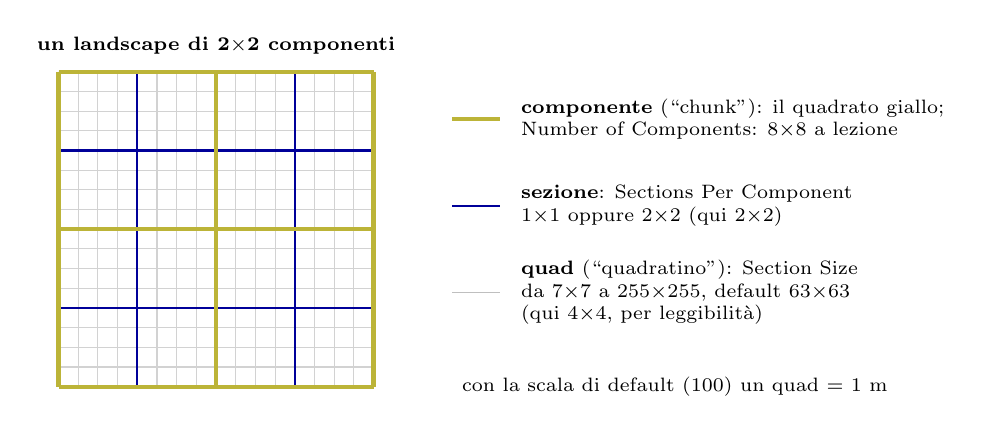
\begin{tikzpicture}[font=\footnotesize, x=1cm, y=1cm]
  % landscape 2x2 componenti, ognuno 2x2 sezioni, sezioni 4x4 quad (schematico)
  \begin{scope}
    \draw[gray!35, step=0.25] (0,0) grid (4,4);
    \draw[blue!60!black, thick, step=1] (0,0) grid (4,4);
    \draw[yellow!70!black, ultra thick, step=2] (0,0) grid (4,4);
    \node[anchor=south, font=\scriptsize\bfseries] at (2,4.1) {un landscape di 2$\times$2 componenti};
  \end{scope}
  % legenda
  \begin{scope}[xshift=5cm]
    \draw[yellow!70!black, ultra thick] (0,3.4) -- (0.6,3.4);
    \node[anchor=west, align=left, font=\scriptsize] at (0.75,3.4) {\textbf{componente} (``chunk''): il quadrato giallo;\\Number of Components: 8$\times$8 a lezione};
    \draw[blue!60!black, thick] (0,2.3) -- (0.6,2.3);
    \node[anchor=west, align=left, font=\scriptsize] at (0.75,2.3) {\textbf{sezione}: Sections Per Component\\1$\times$1 oppure 2$\times$2 (qui 2$\times$2)};
    \draw[gray!50] (0,1.2) -- (0.6,1.2);
    \node[anchor=west, align=left, font=\scriptsize] at (0.75,1.2) {\textbf{quad} (``quadratino''): Section Size\\da 7$\times$7 a 255$\times$255, default 63$\times$63\\(qui 4$\times$4, per leggibilità)};
    \node[anchor=west, align=left, font=\scriptsize] at (0,0.0) {con la scala di default (100) un quad = 1 m};
  \end{scope}
\end{tikzpicture}
\caption{La struttura di un landscape. I componenti (i \emph{chunk} gialli della preview)
sono le unità che il motore gestisce separatamente; ogni componente è diviso in una o
quattro sezioni; ogni sezione è una griglia di quad. Più quad significano curve più
morbide e più peso. Schema con valori ridotti per leggibilità.}
\label{ue14:fig:struttura}
\end{figure}

\begin{table}[htbp]
\centering
\small
\begin{tabular}{@{}p{4.2cm}p{3.0cm}p{6.8cm}@{}}
\toprule
\textbf{Parametro} & \textbf{A lezione} & \textbf{Che cosa decide} \\
\midrule
Section Size & 63$\times$63 (default); provati 31$\times$31 e 7$\times$7 & quanti quad ha
ogni sezione: più quad, terreno più morbido e più pesante \\
Sections Per Component & 2$\times$2, poi 1$\times$1 & in quante sezioni è diviso ogni
componente \\
Number of Components & 8$\times$8 & quanti componenti sulle X e sulle Y (landscape lungo,
largo, quadrato) \\
Overall Resolution & ricalcolata & il numero totale di vertici per lato (deriva dai valori
sopra) \\
Location, Rotation, Scale & invariati & la posizione e la dimensione del landscape; la scala
cambia la dimensione dei quad \\
Material & rimandato & il materiale con cui il landscape nasce \\
Fill World & non usato & crea un landscape grande quanto il mondo \\
Edit Layers & visti nella Manage & i livelli di modifica sovrapposti, bloccabili \\
\bottomrule
\end{tabular}
\caption{I parametri di creazione del landscape visti a lezione.}
\label{ue14:tab:creazione}
\end{table}

\paragraph{Approfondimento: i numeri del landscape di default.} Un quad, con la scala di
default (100 su X e Y), misura un metro: è comodo, perché la griglia del terreno coincide
con quella del pavimento della gym. La \emph{Overall Resolution} è il numero di vertici per
lato: con sezioni di 63 quad, una sezione per componente e 8 componenti per lato si hanno
$8 \times 63 + 1 = 505$ vertici, cioè un landscape di 504 metri per lato; con 2$\times$2
sezioni per componente il conto raddoppia ($8 \times 126 + 1 = 1009$). Le dimensioni
ammesse sono quelle della forma $2^n-1$ (7, 15, 31, 63, 127, 255) perché ogni livello di
LOD dimezza i quad di una sezione. Il componente è l'unità che il motore disegna, scarta e
semplifica: componenti più grandi significano meno oggetti da gestire ma un controllo più
grossolano. Epic consiglia di non esagerare con il numero di componenti (qualche migliaio
al massimo) e di scegliere le dimensioni fra quelle raccomandate nella documentazione. I
\emph{layer} della scheda Manage sono gli \textbf{Edit Layers}, attivi di default in
Unreal Engine~5: ogni layer conserva le proprie modifiche di scultura e di pittura, si può
bloccare, nascondere o cancellare senza toccare gli altri, come in un programma di grafica.
Funzionamento generale dell'engine.

% ---------------------------------------------------------------------
\section{Il pennello: falloff, strength, Alpha e Pattern}
\label{ue14:sec:pennello}

Lo strumento con cui si modifica il landscape ``è un cerchio, un pennello''. Cliccando, il
terreno si alza nel punto evidenziato: ``perché si alza? Perché siamo su \textbf{Sculpt} come
tool''. Prima degli strumenti, però, il docente spiega il pennello, che ``lascia anche
questa specie di immagine residua quando passa'' e ha una serie di parametri comuni a quasi
tutti gli strumenti (tabella~\ref{ue14:tab:pennello}).

\paragraph{Size, Falloff e Strength.}
\begin{itemize}
  \item la \textbf{grandezza} del pennello (\emph{Brush Size}), ``quindi effettivamente quanto è
        largo'';
  \item il \textbf{falloff}: ``è la distanza che c'è fra il primo cerchio e il secondo
        cerchio''. Il pennello ha due cerchi concentrici: dentro il primo l'effetto è pieno,
        fra il primo e il secondo sfuma. Con falloff \textbf{0} ``è tutto pieno'', e quando si
        alza qualcosa ``si alza tutto in blocco''; con falloff \textbf{1} ``si alza solo la
        punta e il resto è tutto quanto ammorbidito, è tutta sfumatura'';
  \item la \textbf{strength} (\emph{Tool Strength}), ``la forza del tool'': a 0,1 l'effetto si
        applica lentamente, a 1 molto più in fretta. ``È quanto forte viene applicato lo
        strumento.''
\end{itemize}

\paragraph{I quadratini e lo stretch del materiale.} ``Cosa stiamo vedendo con questi
quadratini a terra?'' La griglia disegnata sul landscape mostra ``il modo in cui sono
strutturati i poligoni'' e quindi, ``di conseguenza, in che modo verrà \textbf{stretchato il
materiale} quando ce l'andiamo a mettere sopra''. Il docente confronta tre zone
(figura~\ref{ue14:fig:stretch}): in piano ``il massimo della fedeltà, della risoluzione''; su
una salita morbida un materiale ``stretchato mediamente, ma rimane compatto''; su una parete
alzata con falloff zero un materiale che ``esplode'', perché il terreno non sale ``dritto per
dritto verticale'': c'è un quad che viene tirato in verticale ``per far sì che un lato sia
sul livello superiore, l'altro lato sul livello inferiore'', e lì il materiale ``sarà tutto
rovinato''.

\paragraph{Le forme del falloff.} Il \emph{Brush Falloff} ha quattro forme
(figura~\ref{ue14:fig:falloff}):
\begin{itemize}
  \item \textbf{Smooth}: ``il fall off è morbido'';
  \item \textbf{Linear} (``sharp linear''): ``non è morbido, ma è lineare, è geometrico'', una
        linea ``che dritta per dritta parte dalla base e arriva verso l'alto'';
  \item \textbf{Spherical}: ``un effetto più bombato'', ``una sorta di collinetta'' che poi
        ``spiove verso il basso'';
  \item \textbf{Tip}, ``il fall off convesso'', l'opposto dello spherical: la base è morbida e
        poi diventa lineare, con un effetto che ricorda ``le montagne dell'isola di Drum'' di
        \emph{One Piece} (``Drummond Island'' nella trascrizione: sono i \emph{Drum
        Rockies}, montagne a colonna).
\end{itemize}
``A seconda della situazione utilizzerete lo strumento più adatto'': linee morbide con lo
spherical, forme più aguzze con il tip.

\paragraph{I Brush Type.} ``Di base, il brush è un semplice \textbf{cerchio}''
(\emph{Circle}). Ma ci sono altri tipi:
\begin{itemize}
  \item l'\textbf{Alpha}: ``ora il nostro pennello non è più un cerchio, è una
        \textbf{texture}''. Si sceglie la texture dalla lista e ``funziona esattamente come
        avevamo fatto per i materiali: ci sono degli 0 e degli 1'': il pennello alza i bianchi
        e lascia a terra i neri. Con una texture di prova fatta di due quadrati bianchi e due
        neri si vede bene; il pennello \textbf{ruota} seguendo il movimento perché è attivo
        l'\emph{Auto Rotate}, che si può disattivare. L'uso tipico è con le texture di
        \textbf{noise}, che creano ``disturbo'': troppo, se esagerato, ma ``può esservi utile
        per andare a creare un effetto montagnoso, zigrinato, che dalla distanza può essere
        piacevole alla vista''. Qui si possono cambiare solo la grandezza e poco altro;
  \item il \textbf{canale} della texture (\emph{Texture Channel}), disponibile sia nell'Alpha
        sia nel Pattern. Il docente ripassa i canali, visti ``alla prima lezione che avevo
        fatto'': una texture ha i canali \textbf{RGB}, e i grafici li usano ``per mettere più di
        un'informazione all'interno della stessa texture'', come nelle mappe \textbf{ORM}
        (\emph{ambient occlusion} nel rosso, \emph{roughness} nel verde, \emph{metallic} nel
        blu). Il pennello può usare solo il rosso, solo il verde o solo il blu; con il noise
        ``saranno tutte uguali'';
  \item il \textbf{Pattern}: ``un portare all'estremo quello che faceva l'alfa''. La texture
        non è più ``messa su un quadrato'' ma proiettata sotto un pennello circolare, ``una
        fusione delle due precedenti'', e si può modificare: la \textbf{scala} (più piccola,
        ``molta più differenza nella costruzione''), la \textbf{rotazione}, le \textbf{U} e le
        \textbf{V}, ``quindi il \emph{panning}'', cioè lo scorrimento della texture.
        L'esempio: ``la faccia di Marte'', la collina che sembra un volto: con una texture a
        forma di faccia ``sembra che il terreno sia costruito in forma di faccia'';
  \item il \textbf{Component}, ``che io non ho mai usato, per essere onesto'': lavora
        direttamente sui componenti, per esempio per alzare un singolo chunk. Utile per
        dividere il landscape in due zone, ``una zona superiore e una zona inferiore'', che il
        giocatore dovrà collegare ``facendo X cose''.
\end{itemize}

\begin{figure}[htbp]
\centering
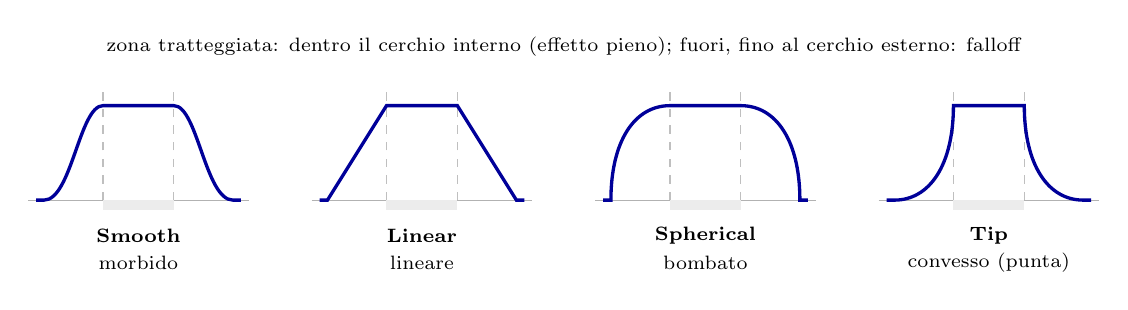
\begin{tikzpicture}[font=\footnotesize, x=1cm, y=1cm]
  \foreach \i/\name/\desc in {0/Smooth/morbido, 1/Linear/lineare, 2/Spherical/bombato, 3/Tip/convesso (punta)} {
    \begin{scope}[xshift=\i*3.6cm]
      \draw[gray!60] (-1.4,0) -- (1.4,0);
      \fill[gray!15] (-0.45,-0.12) rectangle (0.45,0);
      \draw[gray!50, dashed] (-0.45,0) -- (-0.45,1.4) (0.45,0) -- (0.45,1.4);
      \node[font=\scriptsize\bfseries] at (0,-0.45) {\name};
      \node[font=\scriptsize] at (0,-0.8) {\desc};
    \end{scope}
  }
  % Smooth: cosine
  \draw[very thick, blue!60!black] (-1.3,0) -- (-1.2,0) .. controls (-0.85,0) and (-0.75,1.2) .. (-0.45,1.2) -- (0.45,1.2) .. controls (0.75,1.2) and (0.85,0) .. (1.2,0) -- (1.3,0);
  % Linear
  \begin{scope}[xshift=3.6cm]
    \draw[very thick, blue!60!black] (-1.3,0) -- (-1.2,0) -- (-0.45,1.2) -- (0.45,1.2) -- (1.2,0) -- (1.3,0);
  \end{scope}
  % Spherical
  \begin{scope}[xshift=7.2cm]
    \draw[very thick, blue!60!black] (-1.3,0) -- (-1.2,0) .. controls (-1.2,0.75) and (-0.9,1.2) .. (-0.45,1.2) -- (0.45,1.2) .. controls (0.9,1.2) and (1.2,0.75) .. (1.2,0) -- (1.3,0);
  \end{scope}
  % Tip
  \begin{scope}[xshift=10.8cm]
    \draw[very thick, blue!60!black] (-1.3,0) -- (-1.2,0) .. controls (-0.75,0) and (-0.45,0.45) .. (-0.45,1.2) -- (0.45,1.2) .. controls (0.45,0.45) and (0.75,0) .. (1.2,0) -- (1.3,0);
  \end{scope}
  \node[font=\scriptsize, align=center] at (5.4,1.95) {zona tratteggiata: dentro il cerchio interno (effetto pieno); fuori, fino al cerchio esterno: falloff};
\end{tikzpicture}
\caption{Le quattro forme del \emph{Brush Falloff}, viste in sezione dopo aver alzato il
terreno con lo stesso pennello. Smooth sfuma in modo morbido, Linear con una rampa
dritta, Spherical con una collinetta bombata che spiove all'esterno, Tip con una base
morbida e una punta ripida. Profili schematici.}
\label{ue14:fig:falloff}
\end{figure}

\begin{figure}[htbp]
\centering
\begin{tikzpicture}[font=\footnotesize, x=1cm, y=1cm]
  % profilo del terreno con griglia di quad (vista laterale)
  \draw[gray!50] (0,0) -- (12,0);
  % piano
  \foreach \x in {0,0.5,...,3.5} {\draw[thick, green!40!black] (\x,0) -- (\x+0.5,0); \fill[green!40!black] (\x,0) circle (0.04);}
  \node[font=\scriptsize, align=center] at (2,-0.6) {piano: quad regolari\\``massima fedeltà''};
  % salita morbida
  \draw[thick, orange!80!black] (4,0) -- (4.5,0.15) -- (5,0.4) -- (5.5,0.7) -- (6,0.95) -- (6.5,1.1) -- (7,1.15);
  \foreach \p in {(4,0),(4.5,0.15),(5,0.4),(5.5,0.7),(6,0.95),(6.5,1.1),(7,1.15)} {\fill[orange!80!black] \p circle (0.04);}
  \node[font=\scriptsize, align=center] at (5.5,-0.6) {salita morbida:\\stretch medio};
  % parete
  \draw[thick, red!70!black] (7,1.15) -- (7.5,1.15) -- (8,1.15) -- (8.5,3.0) -- (9,3.0) -- (9.5,3.0);
  \foreach \p in {(7.5,1.15),(8,1.15),(8.5,3.0),(9,3.0),(9.5,3.0)} {\fill[red!70!black] \p circle (0.04);}
  \draw[red!70!black, thick] (8,1.15) -- (8.5,3.0);
  \node[font=\scriptsize, align=center, red!70!black] at (10.6,2.1) {un solo quad tirato\\in verticale: il\\materiale ``esplode''};
  \draw[-{Stealth[length=2mm]}, red!70!black] (9.7,2.1) -- (8.35,2.1);
  % texture schematica sopra la parete
  \foreach \t in {0.15,0.3,...,0.9} {\draw[red!40] ($(8,1.15)!\t!(8.5,3.0)$) -- ++(0.12,0);}
  \node[font=\scriptsize, align=center] at (8.5,-0.6) {parete con falloff 0:\\stretch estremo};
  % smooth
  \draw[-{Stealth[length=2mm]}, thick, blue!60!black] (10.4,1.0) -- (11.6,1.0);
  \node[font=\scriptsize, align=center, blue!60!black] at (11.0,0.35) {Smooth:\\quad più\\proporzionati};
\end{tikzpicture}
\caption{Lo \emph{stretch} del materiale, visto di lato. I punti sono i vertici della
griglia del landscape, a distanza fissa in pianta: in piano i quad sono regolari, su una
salita morbida si allungano un po', su una parete alzata in blocco un solo quad copre tutto
il dislivello e la texture si stira fino a diventare illeggibile. Lo strumento Smooth
riavvicina le proporzioni. Ricostruzione schematica.}
\label{ue14:fig:stretch}
\end{figure}

\begin{table}[htbp]
\centering
\small
\begin{tabular}{@{}p{3.6cm}p{10.4cm}@{}}
\toprule
\textbf{Parametro} & \textbf{Che cosa fa} \\
\midrule
Brush Size & la grandezza del pennello \\
Brush Falloff & la parte sfumata fra il cerchio interno e quello esterno: 0 tutto pieno, 1
tutto sfumato \\
Tool Strength & quanto in fretta e quanto forte si applica l'effetto (0,1 lento, 1 forte) \\
Falloff: Smooth, Linear, Spherical, Tip & la forma della sfumatura: morbida, lineare,
bombata, convessa a punta \\
Brush Type: Circle & il pennello circolare di base \\
Brush Type: Alpha & una texture come pennello: alza i bianchi, lascia i neri; Auto Rotate
lo fa ruotare con il movimento \\
Texture Channel & quale canale della texture usare (R, G o B) \\
Brush Type: Pattern & una texture proiettata sotto il pennello circolare, con scala,
rotazione e panning U/V \\
Brush Type: Component & agisce su interi componenti \\
\bottomrule
\end{tabular}
\caption{I parametri del pennello del Landscape Mode, comuni a quasi tutti gli
strumenti di scultura e di pittura.}
\label{ue14:tab:pennello}
\end{table}

\paragraph{Approfondimento: perché la parete ``esplode''.} Il landscape, essendo un
\emph{heightfield}, ha i vertici a distanza fissa in pianta: alzare un punto ne cambia solo
l'altezza, non la posizione orizzontale. Un dislivello di dieci metri fra due vertici
distanti un metro produce un quad lungo più di dieci metri e largo uno, e la texture,
mappata di default dall'alto (proiezione planare sul piano XY), vi si stira di dieci volte.
I rimedi sono tre: evitare pendenze troppo ripide (lo Smooth, che il docente chiama ``il
miglior amico dei vostri materiali''), usare nel materiale una proiezione che tenga conto
delle pareti (la proiezione \emph{triplanare} o \emph{world aligned}, che il materiale
StackOBot usa con la Absolute World Position), oppure coprire le pareti verticali con
delle mesh di roccia, come si fa quasi sempre nelle produzioni reali. Funzionamento
generale dell'engine.

% ---------------------------------------------------------------------
\section{La domanda sulle caverne}
\label{ue14:sec:caverne}

``C'è qualcosa che volevi chiedere per ora? Prima dicevi delle caverne che non si possono
fare.'' Uno studente ha provato a smanettare: è \textbf{impossibile fare dei buchi nel
landscape} con questi strumenti. Il docente conferma: ``per fare un buco avete bisogno dello
strumento \textbf{Visibility}, della \textbf{visibility mask}''. Ma la visibility mask ``si
modifica dal materiale del landscape'': bisogna aggiungere al materiale dei nodi specifici,
e solo allora si potrà avere una parte di landscape attraversabile, ``in cui possiamo andare
a costruire delle caverne''.

Lo studente pensava ad \textbf{Astroneer}, in cui scavare il terreno è la meccanica
principale. Il docente distingue due logiche: ``quando vai a creare un gioco devi far sì che
l'editor per il giocatore sia più \emph{user friendly} possibile''; ``quando stai creando un
editor, forse ti preoccupi di avere più possibilità possibili a disposizione''. Il buco ``si
può fare, non si può fare da qui''. In anteprima mostra lo strumento Visibility: il pennello
è \textbf{rosso} e cliccando non fa nulla, perché in basso Unreal avverte che il
\emph{visibility painting} è disabilitato: il componente ``non ha il nodo \textbf{Landscape
Visibility Mask} nel materiale''. Lo si vedrà a fine lezione
(sezione~\ref{ue14:sec:visibility}).

\paragraph{Approfondimento: terreni scavabili.} Giochi come Astroneer non usano un
heightfield ma un terreno \emph{volumetrico} (voxel), in cui ogni punto dello spazio sa se è
pieno o vuoto, e la superficie viene ricostruita a ogni modifica: per questo vi si possono
scavare tunnel e caverne in gioco. Il landscape di Unreal non funziona così, e una grotta
si fa nascondendo una porzione di terreno con la Visibility e costruendo l'interno con
delle mesh. Per terreni scavabili in Unreal esistono plugin di terzi basati sui voxel.
Funzionamento generale dell'engine.

% ---------------------------------------------------------------------
\section{Gli strumenti di scultura: Sculpt, Erase, Smooth, Flatten}
\label{ue14:sec:sculpt}

``Cosa fanno i nostri pennellozzi?'' ``Ognuno di voi troverà il modo con cui si trova più
comodo a fare le cose''; il docente mostra solo che cosa fa ogni strumento della scheda
\textbf{Sculpt} (tabella~\ref{ue14:tab:sculpt}).

\paragraph{Sculpt.} ``Il più semplice delle cose semplici'': scolpisce, alza il terreno. Ma,
come si è visto ``diverse volte per sbaglio'', non va solo verso l'alto: \textbf{Shift +
clic sinistro} ``scava'', e crea ``delle zone interrate'', delle depressioni.

\paragraph{Erase.} Cancella: ``elimina tutte le modifiche che abbiamo fatto, che siano verso
l'alto o verso il basso''. (Dopo la pausa il docente nota che anche l'Erase rispetta il
falloff: cancella ``in maniera sfumata'' le parti che cadono nella sfumatura.)

\paragraph{Smooth.} ``Ammorbidisce. Immaginatevelo come uno strumento che crea
sfumature.'' Se il pennello prende sia una parte alta sia una parte bassa, cliccando ``crea
una discesa più morbida'': ``fa una media, alza le parti abbassate, abbassa le parti un
pochino più alte'' e produce una \emph{slope} più leggera. ``Lo strumento Smooth è il miglior
amico dei vostri materiali'': ricordando che quanto sono stirati i quadratini ``è anche quanto
saranno stretchati i materiali'', uno smoothing li rende ``sempre più proporzionati''. Con un
pennello più grande della cima, però, ``lui abbassa proprio tutto''; per i ``lavori di fino''
si rimpicciolisce il pennello e si fanno piccole modifiche ``che non vanno a sbragare
completamente tutta la parete''. Anche qui ci sono falloff, tipi di pennello e strength, e
un parametro in più per la \textbf{precisione} dello smoothing (il \emph{Detail Smooth}):
``più grande è questo valore, più dettagli vengono rimossi'', più piccolo, ``meno dettagli
vengono rimossi''. I ``dettagli'' sono ``tutti questi su e giù'': con un valore alto e un
pennello grande ``lui pialla tutto'', con un valore piccolo i cambiamenti sono ``molto
morbidi'' e ``molto precisi''; ``a zero chiaramente non farà mai nulla''.

\paragraph{Flatten.} ``Il mio strumento preferito.'' Il docente si costruisce ``un piccolo
parco giochi'' di colline per gli esempi. Il \textbf{Flatten} ``ci permette di selezionare un
punto e appiattire tutto quanto a quell'altezza'': si clicca dove c'è la croce e tutto ciò
che passa sotto il pennello viene portato a quell'altezza, sia in basso sia sulla vetta.
Serve a una ``terraformazione un po' più controllata'':
\begin{itemize}
  \item \textbf{plateau}, altopiani: il ``lenzuolo'' tirato su si interrompe al bordo,
        ``non riscende giù'';
  \item \textbf{scaloni}, cliccando su punti diversi di una slope: ``scalone, altro scalone,
        altro scalone'', ``delle formazioni un po' più sensate, un po' più normali'', da
        ammorbidire poi con lo Smooth. Per esempio ``le cascatine fatte a livelli'' o ``le
        \textbf{risaie}'', con parti piatte e parti rialzate;
  \item un \textbf{canyon} dentro una parte rialzata: un fondo appiattito e i lati rimasti
        alti.
\end{itemize}

\paragraph{Le modalità del Flatten.} ``È abbastanza brutale come strumento, perché prende e
appiattisce tutto'': si rischia di appiattire le cose sbagliate. Per questo c'è la
\textbf{Flatten Mode} (figura~\ref{ue14:fig:flatten}):
\begin{itemize}
  \item \textbf{Both} (default): ``alza i piani che stanno più in basso e abbassa i piani che
        stanno più in alto'';
  \item \textbf{Raise}: alza tutti i punti fino all'altezza scelta, ``però non abbassa''.
        Esempio: un rilievo che fa da \textbf{bordo della mappa} resta intatto, e si alza
        solo ciò che c'è sotto;
  \item \textbf{Lower}: abbassa ``tutto quello che c'è da abbassare, ma non alza'': ``se c'è
        una grotta o un canyon che deve rimanere giù, non lo tira più su''.
\end{itemize}
``Principalmente questi sono i due che vorrete utilizzare, perché sono quelli che vi danno
un po' più di controllo.'' Di un'altra opzione il docente legge a fatica il nome (``height
intervals'', ``specification at intervals''): ``questo è uno che effettivamente non ho mai
utilizzato''. Si tratta, con ogni probabilità, della modalità \textbf{Terrace} (si veda
l'approfondimento).

\paragraph{Use Slope Flatten.} Con la casella \textbf{Use Slope Flatten}, invece di
appiattire in orizzontale ``andate a continuare il piano diagonale preso originariamente'':
cliccando su un pendio, lo strumento prolunga quella pendenza, ``anche scavando verso il
basso''. Serve per ``quei pianori, quegli spiazzi montani'' che sono ``uno spaccato dritto per
dritto, che però va in diagonale''. Ultimo uso, personale: ``a volte il Flatten tendo a
utilizzarlo tipo \textbf{gomma}'': si punta sul livello base del landscape e si appiattisce.

``Abbiamo visto scolpire, tirare su, tirare giù, ammorbidire, cancellare e appiattire.''

\begin{figure}[htbp]
\centering
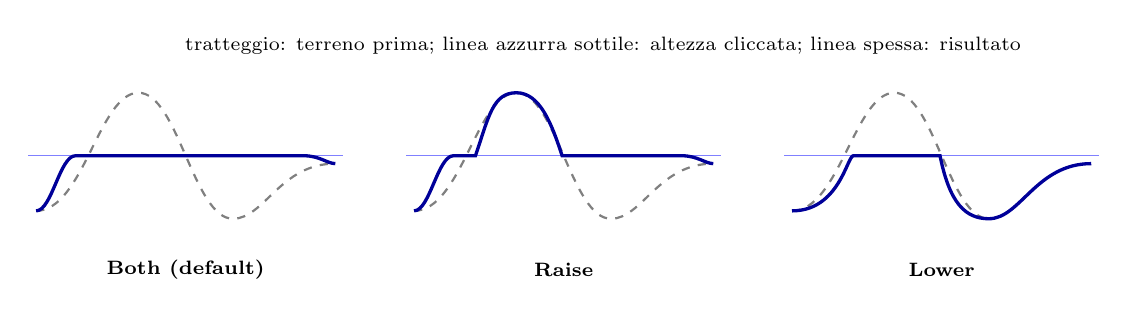
\begin{tikzpicture}[font=\footnotesize, x=1cm, y=1cm]
  \foreach \i/\name in {0/Both (default), 1/Raise, 2/Lower} {
    \begin{scope}[xshift=\i*4.8cm]
      % profilo originale
      \draw[gray, dashed, thick] (0,0.3) .. controls (0.6,0.3) and (0.8,1.8) .. (1.3,1.8) .. controls (1.8,1.8) and (2.0,0.2) .. (2.5,0.2) .. controls (2.9,0.2) and (3.1,0.9) .. (3.8,0.9);
      \draw[blue!50, thin] (-0.1,1.0) -- (3.9,1.0);
      \node[font=\scriptsize, blue!60!black, anchor=west] at (3.9,1.0) {};
      \node[font=\scriptsize\bfseries] at (1.9,-0.45) {\name};
    \end{scope}
  }
  % Both: tutto a 1.0
  \draw[very thick, blue!60!black] (0,0.3) .. controls (0.2,0.3) and (0.3,1.0) .. (0.5,1.0) -- (3.4,1.0) .. controls (3.6,1.0) and (3.7,0.9) .. (3.8,0.9);
  % Raise: alza le valli, non abbassa la cima
  \begin{scope}[xshift=4.8cm]
    \draw[very thick, blue!60!black] (0,0.3) .. controls (0.2,0.3) and (0.3,1.0) .. (0.5,1.0) -- (0.78,1.0) .. controls (0.95,1.5) and (1.0,1.8) .. (1.3,1.8) .. controls (1.6,1.8) and (1.75,1.4) .. (1.88,1.0) -- (3.4,1.0) .. controls (3.6,1.0) and (3.7,0.9) .. (3.8,0.9);
  \end{scope}
  % Lower: abbassa la cima, non alza le valli
  \begin{scope}[xshift=9.6cm]
    \draw[very thick, blue!60!black] (0,0.3) .. controls (0.6,0.3) and (0.7,1.0) .. (0.78,1.0) -- (1.88,1.0) .. controls (2.0,0.4) and (2.2,0.2) .. (2.5,0.2) .. controls (2.9,0.2) and (3.1,0.9) .. (3.8,0.9);
  \end{scope}
  \node[font=\scriptsize, align=center] at (7.2,2.4) {tratteggio: terreno prima; linea azzurra sottile: altezza cliccata; linea spessa: risultato};
\end{tikzpicture}
\caption{Le tre modalità principali del Flatten, in sezione. Both porta tutto all'altezza
cliccata; Raise alza solo ciò che sta sotto e lascia la cima (per esempio il bordo della
mappa); Lower abbassa solo ciò che sta sopra e lascia le valli (per esempio un canyon).
Profili schematici.}
\label{ue14:fig:flatten}
\end{figure}

\paragraph{Approfondimento: Terrace e gli altri parametri del Flatten.} Nella versione di
Unreal Engine~5 il Flatten ha quattro modalità: oltre a Both, Raise e Lower, la modalità
\textbf{Terrace}, che appiattisce il terreno a \emph{intervalli} di altezza regolari
(\emph{Terrace Interval}), con una sfumatura fra un gradino e l'altro (\emph{Terrace
Smooth}): è lo strumento giusto per le risaie e le cascate a livelli che il docente
costruisce a mano cliccando su più punti. Altri parametri utili: \emph{Pick Value Per
Apply}, che ricampiona l'altezza a ogni pennellata invece di tenere quella del primo clic;
\emph{Flatten Target}, che permette di scrivere a mano l'altezza a cui appiattire (comodo
per avere esattamente le misure della gym, per esempio un plateau a 1,40 m sopra un
altro); e \emph{Show Preview Grid}, che mostra il piano di destinazione. Funzionamento
generale dell'engine; la lezione non li tocca.

% ---------------------------------------------------------------------
\section{Ramp e i LOD}
\label{ue14:sec:ramp}

``Adesso vediamo uno strumento che funziona in maniera un po' diversa. Non è più un
pennello, ma dei clic'': lo strumento \textbf{Ramp}. Si clicca su due punti, li si sposta
come si vuole, e quando si è contenti si preme \textbf{Add Ramp}: Unreal aggiunge ``un
collegamento di landscape da punto A a punto B''. Il docente chiede alla classe che cosa
succederà con due punti sul fondo di due valli separate da una collina: ``ti farà un canyon
lì in mezzo'' (la rampa porta il terreno ``sempre da punto A a punto B'', anche scavando).

\paragraph{Gli usi.}
\begin{itemize}
  \item una \textbf{rampa} per salire su un punto sopraelevato (``sarà un modo molto brutto,
        però va'');
  \item le rampe di un gioco di \textbf{macchine} o di \textbf{skateboard};
  \item ``una \textbf{diga} in un crepaccio'', un collegamento pieno da una parte all'altra.
\end{itemize}
Un \textbf{ponte sospeso}, invece, no. Si potrebbe pensare di fare la diga e poi bucarla
sotto con la Visibility, ``tuttavia ci sarebbe un problema'': la parte sotto non
collegherebbe più le due metà, ``perché il landscape \textbf{non può essere sovrapposto}'',
``non può esserci una parte qui e una parte sotto''. ``Se volete fare un ponte sospeso,
fatelo con le \textbf{mesh}: prendete una mesh, ingranditela e mettetela sopra un crepaccio.
Non fatelo con il landscape.''

\paragraph{Larghezza e falloff.} La rampa ha la sua \textbf{larghezza} (\emph{Ramp Width}),
``se un ponticello, se una grossa salita'', e il suo \textbf{falloff} (\emph{Side Falloff}):
a zero non c'è sfumatura e i lati vengono stirati ``a blocco''; tutto sfumatura, e il
terreno attorno si raccorda morbido. Ma se si ``tira la corda'', con molta sfumatura e una
rampa molto stretta, ``vi si spacca un po' il landscape'': ``questa cosa è molto rotta, e
dalla distanza sarà tremenda'', ``perché i \textbf{LOD} vanno a semplificare il landscape''.

\paragraph{I LOD.} ``Sapete che cos'è un LOD?'' \textbf{LOD} sta per \emph{Level of Detail}.
Un grafico crea una mesh, poniamo da 10.000 poligoni; questa mesh deve avere ``altre
versioni di sé più grezze'', da 5.000, da 2.000 poligoni, perché l'engine, ``e non solo in
automatico'', aggiorna il numero di poligoni ``a seconda della distanza da cui lo vedi''.
L'esempio della statua: da vicino deve essere ``super bellissima'', ma da lontano ``non serve
che abbia ancora 500.000 poligoni'', perché l'occhio non vedrà il dettaglio, e ridurli
alleggerisce le prestazioni. Le distanze si possono impostare (``a 10 metri un tot, a 20
metri un altro tot, a 40 metri un altro tot''), da un Blueprint o dalla mesh stessa. Il
landscape funziona allo stesso modo: dalla distanza i suoi poligoni vengono semplificati.
Una massa grande non ne soffre, ``perché ci sono molti poligoni''; una rampa sottilissima,
``costituita di troppi pochi poligoni, viene distrutta dai LOD''. ``Quindi evitate di fare
delle robe in questo modo.''

\paragraph{Lo sfogo sui Pokémon.} L'esempio, dichiaratamente polemico: i recenti Pokémon
open world, \emph{Scarlatto e Violetto} e \emph{Leggende Pokémon: Arceus}. ``Potete vedere
attivamente la terra che si muove, come se fosse animata'': ``sono semplicemente i LOD che si
attivano troppo presto'', il landscape ``viene semplificato con troppo anticipo''. Il
motivo, secondo il docente, è l'ottimizzazione: se in una visione ampia si vedesse tutto
con tutti i poligoni ``esploderebbe la console''. ``Non è che sono brutte, ma è che sono
troppo ottimizzate, e la troppa ottimizzazione le rende orribili''; e sono così ottimizzate
``perché il gioco è programmato in maniera talmente stupida da essere pesante''. ``Scusate
questo piccolo sfogo contro Game Freak.'' (È un giudizio personale del docente, non
un'analisi tecnica verificata; il fenomeno del terreno che ``si muove'' quando cambia il LOD,
il \emph{LOD popping}, è comunque reale e ben noto.)

\paragraph{La regola.} ``Diamo sempre un po' di spazio al landscape'': niente forme troppo
sottili. ``Questo è anche il motivo per cui vorremmo evitare dei landscape troppo piccoli'':
un landscape 7x7 ``capita molto spesso che si spacchi in questo modo, perché ha pochi
poligoni a disposizione''. Il docente rifà ``una rampina decente''.

\paragraph{Approfondimento: i LOD del landscape.} Il landscape non ha LOD costruiti a mano
come una static mesh: li calcola da solo, dimezzando a ogni livello i quad di ogni sezione
(per questo le Section Size sono della forma $2^n-1$). La transizione è regolata da
parametri dell'actor Landscape (in Unreal Engine~5 \emph{LOD 0 Screen Size}, \emph{LOD 0
Distribution Setting} e \emph{LOD Distribution Setting}, più eventuali \emph{LOD Group}),
che decidono a quale dimensione sullo schermo un componente passa al livello successivo.
Aumentarli rende il terreno lontano più fedele e più costoso. Le forme più sottili di una
sezione, come la rampa stretta del docente, sono le prime a sparire perché nel livello
semplificato non ci sono più vertici abbastanza vicini per descriverle. Il capitolo 12 di
Romero e Sewell, sulla pubblicazione, ricorda che fra le impostazioni di scalabilità del
gioco c'è anche la qualità del \emph{foliage}, e che se le prestazioni calano solo in certe
zone del livello conviene ``ridurre la densità degli oggetti'' o la qualità di un modello:
il compromesso fra dettaglio e prestazioni di cui parla il docente. Per la parte sui
parametri del landscape, funzionamento generale dell'engine.

% ---------------------------------------------------------------------
\section{Erosion, Hydro, Noise, Mirror e Copy/Paste}
\label{ue14:sec:altristrumenti}

\paragraph{Erosion e Hydro.} ``Sono due strumenti con cui io faccio un po' a botte'' (``a
volte'' nella trascrizione, ma il seguito chiarisce il senso): il
docente spiega a che cosa servirebbero e perché non gli piacciono. L'idea è ``simulare
delle deformazioni, del \emph{displacement}''. L'\textbf{Erosion} è lo strumento con cui
``andrei a dettagliare una parete montuosa'': ``è un po' il contrario dello smooth'', crea
nel pennello parti rialzate e parti abbassate. (Qui la trascrizione si interrompe in una
frase ripetuta; riprende con la domanda di uno studente.)
\begin{itemize}
  \item il \textbf{Threshold} ``va a definire quanta differenza fra punto A e punto B deve
        esserci per andare a fare erosione'': con un valore alto l'erosione si applica solo
        dove il dislivello è grande; abbassandolo (``tipo 17'') si erode ``molto di più, in
        molti punti diversi'', perché basta una differenza minore;
  \item \textbf{Noise Mode} e \textbf{Noise Scale} aggiungono un rumore preimpostato, e come
        nel Flatten si sceglie se deve alzare e abbassare, solo alzare o solo abbassare.
\end{itemize}
L'\textbf{Hydro} (\emph{Hydro Erosion}) ``funziona più o meno nello stesso modo'' e
vorrebbe creare un \emph{displacement} ``stile fondali marini'' o ``erosione dell'acqua''. Il
problema è che ``abbiamo un po' poco controllo'': ``io non sono mai riuscito a farlo
funzionare bene, proprio non mi trovo''.

\paragraph{Noise.} ``Preferisco piuttosto utilizzare il \textbf{Noise}'', che ``fa rumore'' e
permette di scegliere se aggiunge, se toglie o se fa entrambe le cose. Con un pennello
grande e la scala del noise ridotta, ``vi va a fare una deformazione un po' più subdola'':
``non prende e spacca, ma fa dei leggeri movimenti di alzare e abbassare'', il risultato
``che al mio occhio è sempre il più piacevole''. In modalità solo-aggiunta il Noise alza,
``però non come lo Sculpt'' (aggiunge rumore, non una collina); lo stesso vale per la
sottrazione.

\paragraph{Gli strumenti saltati.} ``Facciamo al volissimo le ultime cose'':
\begin{itemize}
  \item il \textbf{Retopologize} ``non ci interessa'';
  \item la \textbf{Visibility}, già vista, si riprende più avanti;
  \item il \textbf{Blueprint Brush}, ``qualcosa che onestamente non ho mai utilizzato'':
        ``presumo sia un brush che può essere programmato'' per fare cose specifiche. ``Non
        l'ho mai trovato necessario.''
\end{itemize}

\paragraph{Mirror.} Il \textbf{Mirror} serve ``nel momento in cui avete degli ambienti molto
grandi che volete copiare, che volete specchiare o che volete ruotare''. Compare un
\textbf{piano}: premendo \textbf{Apply}, tutto ciò che sta da un lato viene copiato
sull'altro, ``appiattendo'' quello che c'era. Il piano si sposta avanti e indietro, e
soprattutto dall'\textbf{Operation} si sceglie il tipo di operazione:
\begin{itemize}
  \item \textbf{-X to +X}: copia il lato sinistro sul destro; \textbf{+X to -X} il contrario;
        lo stesso per \textbf{-Y to +Y} e \textbf{+Y to -Y}. Con una forma qualsiasi si ottiene
        ``una macchia di Rorschach'';
  \item le varianti \textbf{Rotate} (per esempio \emph{Rotate -X to +X}): stessa direzione del
        piano, ``ma operazione diversa'': invece di specchiare, ruota, ``come se prendesse
        questa parte del landscape e la ruotasse nell'altra direzione''. Il risultato è
        uguale, ``ma ruotato''.
\end{itemize}

\paragraph{Copy/Paste.} ``Il copia e incolla, la cosa più semplice del mondo.'' Prima si
seleziona una parte di landscape con lo strumento \textbf{Region Select} (``Select''),
dipingendo la zona con il pennello; per togliere la selezione serve \textbf{Clear Region
Selection}, ``perché se andate da altre parti questo vi rimane sempre selezionato''. Poi,
nello strumento \textbf{Copy/Paste}, \textbf{Ctrl+C} copia la zona in un riquadro (il
\emph{gizmo}) che si può spostare, ruotare e scalare dove si vuole, e \textbf{Ctrl+V} la
incolla, ``modificata, ruotata e anche scalata''. Ci sono comandi per adattare il riquadro
alla selezione e per ripulirlo. La \textbf{Paste Mode} ripete la logica del Flatten:
\begin{itemize}
  \item \textbf{Both}: tutto il riquadro viene portato al livello copiato, la zona di
        destinazione viene abbassata a livello base e la parte copiata rialzata;
  \item \textbf{Raise}: alza soltanto ``le parti che erano più basse'' e non abbassa le altre:
        di una collina copiata sopra un'altra resta solo ``la punta'';
  \item \textbf{Lower}: l'opposto.
\end{itemize}
``Abbiamo effettivamente un po' tutte le cose viste.'' Nessuna domanda: pausa, ``ci becchiamo
alle 55 con il Paint, e quindi i materiali del landscape''.

\begin{table}[htbp]
\centering
\small
\begin{tabular}{@{}p{3.0cm}p{11.0cm}@{}}
\toprule
\textbf{Strumento (Sculpt)} & \textbf{Che cosa fa, e come lo usa il docente} \\
\midrule
Sculpt & alza il terreno; Shift + clic scava \\
Erase & cancella le modifiche (rispetta il falloff) \\
Smooth & fa una media delle altezze; Detail Smooth decide quanto dettaglio togliere; ``il
miglior amico dei materiali'' \\
Flatten & appiattisce all'altezza cliccata; Flatten Mode Both, Raise, Lower (e Terrace);
Use Slope Flatten prolunga il pendio; usato anche come ``gomma'' \\
Ramp & crea una rampa fra due punti (Add Ramp), con Ramp Width e Side Falloff; non per i
ponti sospesi \\
Erosion & dettaglia le pareti erodendo dove il dislivello supera il Threshold; Noise Mode e
Noise Scale; ``poco controllo'' \\
Hydro (Hydro Erosion) & erosione ``ad acqua''; il docente non lo usa \\
Noise & aggiunge o toglie rumore; con scala piccola, deformazioni ``subdole'' \\
Retopologize & non visto (``non ci interessa'') \\
Visibility & nasconde porzioni di terreno; richiede la Landscape Visibility Mask nel
materiale \\
Blueprint Brush & pennelli programmabili; mai usato dal docente \\
Mirror & specchia (-X to +X, \dots) o ruota (Rotate \dots) metà del landscape; Apply \\
Region Select & seleziona una zona col pennello; Clear Region Selection \\
Copy/Paste & Ctrl+C e Ctrl+V di una zona, con gizmo spostabile, ruotabile, scalabile;
Paste Mode Both, Raise, Lower \\
\bottomrule
\end{tabular}
\caption{Gli strumenti della scheda Sculpt del Landscape Mode, nell'ordine della lezione.}
\label{ue14:tab:sculpt}
\end{table}

\paragraph{Approfondimento: il terreno come spazio di gioco.} Gli strumenti di scultura
sono tecnici, ma le forme che producono sono categorie di level design. Totten, nel
capitolo 3, osserva che in un open world fatto di paesaggi aperti, come \emph{Skyrim}, i
percorsi fra città e dungeon ``sono molto meno diretti'' e spesso ``campi aperti'': il
giocatore traccia da sé le scorciatoie fra i landmark, ma ``rischia di perdersi'', e i
designer usano ``elementi geografici sottili come sentieri sterrati, cartelli o fiumi'' per
suggerire i percorsi. E aggiunge proprio a proposito degli ``editor di terreno integrati
nell'engine'': tenere a mente queste linee guida serve a creare mondi ``non solo
esteticamente attraenti, ma anche utilizzabili''. Il canyon del Flatten, la diga della Ramp
e il bordo di mappa preservato dal Raise sono, in questi termini, un percorso, un
collegamento e un \emph{edge}; il plateau è un'area in cui il giocatore guarda lontano (il
\emph{prospect space} dello stesso capitolo). Le misure, infine, vengono dalla gym: un
canyon che deve essere invalicabile avrà pareti oltre il Walkable Floor Angle del
personaggio, un plateau raggiungibile con un salto starà sotto l'altezza comoda misurata.

% ---------------------------------------------------------------------
\section{La pausa e la domanda su The Sims}
\label{ue14:sec:pausa}

Alla ripresa (``Guido c'è, Federico c'è, Giulia c'è'') il docente chiede se sia tutto
chiaro: ``è abbastanza semplice, è più una questione di prenderci la mano''. Consiglia di
usare il landscape ``fra questa lezione e la prossima'' per familiarizzare e trovare il
proprio modo di lavorare: ``magari siete dei pazzi completi e lavorate utilizzando soltanto
lo Sculpt, ma siete fortissimi. Io vi dico quali sono i tool, poi voi trovate il vostro
modo di lavoro''.

\paragraph{The Sims.} Uno studente chiede se il terreno della serie \textbf{The Sims}, ``soprattutto
del 2'', sia fatto allo stesso modo. Il docente non lo sa: ``non so con cosa è stato fatto''.
Dopo un rapido controllo: ``a quanto risulta, ogni The Sims ha usato un \textbf{engine custom}''.
È ``plausibile'' che funzioni in modo simile, e che ci sia stata ``una \emph{cross
contamination}, delle influenze da entrambe le parti'': magari anche Unreal si è ispirato a
come ``diversi tycoon o diversi simulatori'' gestivano la terraformazione, perché ``quel tipo
di modifica spaziale è molto comodo farla con un pennello''. ``Non ti so dire di più'':
l'ultima volta che ha giocato a The Sims ``probabilmente era vent'anni fa''. Lo invita a fare
una ricerca e a riferire la volta successiva. (Nello scambio, alla domanda ``quando è uscito
The Sims 2?'', la risposta è ``nel 2000'': in realtà nel 2000 è uscito il primo
\emph{The Sims}; \emph{The Sims 2} è del 2004.)

% ---------------------------------------------------------------------
\section{Il Paint e il materiale del landscape di StackOBot}
\label{ue14:sec:paint}

``Abbiamo visto il Manage, abbiamo visto lo Sculpt, rimane soltanto da vedere il
\textbf{Paint}.'' La scheda ha ``più o meno gli stessi strumenti che c'erano di là'':
\textbf{Paint}, \textbf{Smooth}, \textbf{Flatten} e \textbf{Noise}, con la stessa strength e
gli stessi tipi di pennello. Ma in basso Unreal avverte: \emph{non ci sono target layer
assegnati a questo landscape; usa i bottoni in alto per aggiungerne di nuovi o popolarli
dal materiale correntemente assegnato}. I bottoni sono \textbf{Create Layer} e
\textbf{Create Layers from Assigned Materials}, quest'ultimo, ``se non sbaglio, unico di
Unreal 5, sulla quarta edizione non c'è''.

\paragraph{Un materiale normale non basta.} Il landscape può \textbf{dipingere il materiale}
con il pennello, ``il materiale però deve essere fatto \emph{ad hoc}''. Prova: un nuovo
materiale con dentro ``unicamente un colore''. Messo sul landscape, il landscape lo tratta
``come un oggetto qualsiasi'': ``tutto quanto diventa disgustosamente verde'', e non c'è modo
di modificare nulla, ``perché il nostro materiale di layer non ne ha''.

\paragraph{Il ``grosso errore''.} A questo punto il docente si accorge di ``aver fatto un grosso
errore: niente di grave, semplicemente una cosa che ci farà perdere un po' di tempo'' (la
spiegherà più avanti: sono le Virtual Texture, sezione~\ref{ue14:sec:grass}).

\paragraph{Il pacchetto StackOBot.} Fra gli asset del pacchetto \textbf{StackOBot}, ``il
pacchettino con il robottino e tutte le cose'', nella cartella \emph{Environment} ci sono:
\emph{Props} e \emph{Modular} (mesh da vedere alla fine della lezione ``o all'inizio della
prossima''), \emph{Materials}, \emph{Foliage} (per il Foliage Mode) e \textbf{Landscape}, con
``tutto quello che riguarda il landscape'': delle texture ``che non sappiamo bene cosa
fanno'', una mesh che per ora non serve, dei materiali, fra cui \textbf{M\_Landscape}, e dei
\textbf{Landscape Layers} ``che non sappiamo bene cosa fanno'' e che si rivedranno più
tardi.

\paragraph{Il nero.} Si assegna M\_Landscape al landscape (nel campo \emph{Landscape
Material} dei Details): ``va tutto \textbf{nero}''. Anche un materiale pensato per il
landscape, appena assegnato, ``non ci dà subito quello di cui abbiamo bisogno''; e ``il fatto
che diventi tutto nero è quello che vogliamo, per noi è positivo''. Bisogna stabilire come
funzionano i layer: visto che il materiale ``è già stato costruito per avere tanti layer
diversi'', si preme \textbf{Create Layers from Assigned Materials}. Unreal crea
\textbf{quattro layer}, e il terreno resta nero. (Resta nero perché nessun layer è ancora
stato dipinto: si veda l'approfondimento.)

\paragraph{Dentro M\_Landscape.} Il docente apre il materiale, ``molto piccolo, vero?
Molto comodo'' (ironico: il nodo principale è ridotto a un solo pin). Le parti interessanti:
\begin{itemize}
  \item quattro \textbf{material function}, \emph{MF\_Rocks}, \emph{MF\_Pebbles},
        \emph{MF\_Sand} e \emph{MF\_Grass}: ``il funzionamento dei singoli materiali, quindi
        dei singoli layer''. Si creano con tasto destro, \emph{Material Function}: sono
        ``delle piccole funzioni'', come quelle dei Blueprint, che descrivono ``come funziona
        l'erba, come funziona la ghiaia, i \emph{pebbles}'', la roccia e la sabbia;
  \item dentro ogni funzione le texture sono collegate alla \textbf{Absolute World
        Position}: ``vi ricordate i materiali \textbf{world aligned} che avevamo visto la
        volta scorsa? Questo è il modo per farli, anche per il landscape'';
  \item tutte le funzioni terminano con un nodo \textbf{Set Material Attributes}: un nodo
        ``vuoto'' in cui, aggiungendo slot all'array, si decide quale informazione passa ogni
        ingresso (Base Color, Metallic, Specular, Roughness, Normal\dots). Qui ogni funzione
        passa \textbf{Base Color}, \textbf{Roughness} e \textbf{Normal} del proprio materiale,
        presi da dei \emph{Texture Sample} (``vi ricordate, l'abbiamo fatta questa roba'');
  \item le quattro uscite entrano nel nodo che è ``alla base del funzionamento del
        materiale del landscape'': il \textbf{Landscape Layer Blend}.
\end{itemize}

\paragraph{I nodi del landscape.} Cercando \emph{landscape} nella palette dei nodi, Unreal
mostra ``tutti i nodi che sono utili per il landscape''. Oggi se ne vedono tre (più uno ``che
sta da un'altra parte'', il Landscape Grass Output): il \textbf{Landscape Layer Blend},
``il fondamentale'', il \textbf{Landscape Layer Sample} e la \textbf{Landscape Visibility
Mask}.

\paragraph{Landscape Layer Blend.} È un nodo ``vuoto'', come il Set Material Attributes, in
cui si aggiungono elementi all'array \emph{Layers}. Ogni elemento si apre con delle
freccette, e lì si scrive il \textbf{nome del layer} (per esempio \emph{Grass}).
``Scriveteli bene, perché è importante scrivere bene il nome del layer'': se non c'è il
nome, ``Unreal non lo trova, non lo rileva'', anche se ci sono collegate delle cose; e altri
nodi, come il Landscape Layer Sample, ``hanno bisogno del nome per funzionare''. Gli altri
campi dell'elemento ``sono dei parametri di preview che al momento non ci interessano''.
Usando questo nodo, gli autori del materiale hanno fatto quattro layer: \textbf{roccia},
\textbf{sassolini} (ghiaia), \textbf{sabbia} ed \textbf{erba}, tutti collegati al nodo
risultante del materiale.

\paragraph{Use Material Attributes.} Il nodo risultante è ``così piccolino'' perché nei
dettagli del materiale è spuntata la casella \textbf{Use Material Attributes}, che
``trasforma il modo in cui funziona il nodo'': invece di avere un pin per Base Color, uno per
Roughness, uno per Normal, ha un unico ingresso \emph{Material Attributes}. Senza la casella
bisognerebbe collegare il risultato su ogni parametro, cosa comoda se si vogliono
modificare le singole cose; ma poiché tutte le operazioni avvengono nelle funzioni, ``per
lui è comodo'' far passare tutto in un colpo solo.

\paragraph{Dipingere.} Che cosa permette la suddivisione in layer? ``Di avere dei layer da
poter dipingere.'' Selezionato \textbf{Rock} e passato il pennello, il terreno ``dipinge
roccia'', ``o perlomeno quello che noi abbiamo impostato come valore per il materiale della
roccia'': se non piace, la texture e le dimensioni si cambiano da dentro la sua material
function, ``tutto come abbiamo visto la volta scorsa''. Poi i \textbf{Pebbles} (``dei
sassolini, una ghiaietta''), la \textbf{Sand} e la \textbf{Grass}. Ogni volta Unreal deve
``compilare gli shader'', e ci vuole un po'.

\begin{figure}[htbp]
\centering
\begin{tikzpicture}[font=\scriptsize, x=1cm, y=1cm,
  ue14node/.style={draw, thick, rounded corners=2pt, fill=white, align=center, minimum height=0.6cm, inner sep=3pt},
  ue14fn/.style={ue14node, fill=yellow!15},
  ue14out/.style={ue14node, fill=gray!25, minimum width=2.6cm},
  ue14arr/.style={-{Stealth[length=1.6mm]}, thick}]
  \node[ue14fn] (r) at (0,3.0) {MF\_Rocks};
  \node[ue14fn] (p) at (0,2.2) {MF\_Pebbles};
  \node[ue14fn] (s) at (0,1.4) {MF\_Sand};
  \node[ue14fn] (g) at (0,0.6) {MF\_Grass};
  \node[font=\scriptsize, align=center] at (0,3.9) {material function:\\Texture Sample (World Position)\\$\rightarrow$ Set Material Attributes};
  \node[ue14node, minimum height=3.0cm, minimum width=2.8cm] (lb) at (4.2,1.8) {};
  \node[font=\scriptsize\bfseries] at (4.2,3.55) {Landscape Layer Blend};
  \foreach \n/\y in {Rock/2.6,Pebbles/2.0,Sand/1.4,Grass/0.8} {\node[font=\scriptsize, anchor=west] at (3.0,\y) {Layer \n};}
  \draw[ue14arr] (r.east) -- (3.0,2.6);
  \draw[ue14arr] (p.east) -- (3.0,2.0);
  \draw[ue14arr] (s.east) -- (3.0,1.4);
  \draw[ue14arr] (g.east) -- (3.0,0.8);
  \node[ue14out] (m) at (8.6,1.8) {M\_Landscape\\(Use Material Attributes)\\\emph{Material Attributes}};
  \draw[ue14arr] (lb.east) -- (m.west);
  % grass spawn
  \node[ue14node, fill=green!12] (ls) at (0.6,-1.2) {Landscape Layer Sample\\\emph{Parameter Name: Grass}};
  \node[ue14node] (calc) at (4.2,-1.2) {calcoli\\(GPU Grass Spawn)};
  \node[ue14out, fill=green!25] (go) at (8.6,-1.2) {Landscape Grass Output\\\emph{Grass: GT\_Grass}};
  \draw[ue14arr] (ls.east) -- (calc.west);
  \draw[ue14arr] (calc.east) -- (go.west);
  \node[ue14node, fill=blue!8] (gt) at (8.6,-2.6) {Landscape Grass Type: mesh,\\densità, scala min--max};
  \draw[ue14arr, dashed] (gt.north) -- (go.south);
  \node[font=\scriptsize, align=left, anchor=west] at (-1.4,-2.6) {i nomi \emph{Grass} devono coincidere\\esattamente (maiuscole comprese)};
\end{tikzpicture}
\caption{Lo schema del materiale M\_Landscape di StackOBot come descritto a lezione. In
alto, la parte che \emph{dipinge}: quattro material function entrano nel Landscape Layer
Blend, ognuna nel layer con il proprio nome, e il risultato va al nodo del materiale con
Use Material Attributes. In basso, la parte separata che \emph{fa spawnare} l'erba: un
Landscape Layer Sample legge dove è stato dipinto il layer Grass e, dopo alcuni calcoli,
alimenta il Landscape Grass Output, che usa un Landscape Grass Type. I nodi grigi sono
nodi finali. Ricostruzione schematica.}
\label{ue14:fig:materiale}
\end{figure}

\paragraph{Approfondimento: perché il terreno è nero, e i pesi dei layer.} Un materiale del
landscape non sceglie da solo dove mettere la roccia o l'erba: per ogni layer il landscape
memorizza una \emph{weightmap}, una mappa di pesi da 0 a 1 per ogni vertice, e il Landscape
Layer Blend mescola i layer secondo quei pesi. Appena assegnato il materiale, nessun layer
ha ancora un peso, quindi la somma è zero e il risultato è nero: per questo il docente lo
considera un buon segno. Quando si dipinge il primo layer su un componente, i pesi
cominciano a esistere; dipingere un layer riduce gli altri nello stesso punto, perché in un
layer \emph{weight-blended} la somma dei pesi resta 1. Il primo layer della lista viene
spesso usato come ``fondo'' e si può riempire tutto il terreno con il comando \emph{Fill
Layer} (tasto destro sul layer nella scheda Paint). Ogni layer in più costa: Unreal campiona
le texture di tutti i layer presenti su un componente, e per questo conviene non usarne
troppi per componente. Il pulsante \emph{Create Layers from Assigned Materials} legge i
nomi dei layer dal Landscape Layer Blend del materiale e crea i target layer
corrispondenti; se nel progetto esistono già le relative \emph{Layer Info} (come nel
pacchetto StackOBot) le collega, altrimenti vanno create. Il libro di Romero e Sewell
mostra il Material Editor e i pin Base Color, Metallic e Roughness nel capitolo 5, ma non
tratta i materiali del landscape; il resto si basa sul funzionamento generale dell'engine.

% ---------------------------------------------------------------------
\section{L'erba che spawna e le Virtual Texture}
\label{ue14:sec:grass}

\paragraph{La domanda.} Con l'erba il docente si ferma: ``se mi state seguendo passo passo,
noterete una differenza rispetto a quella che ho io''. ``Vi sembra che quello che ha fatto
sia uguale a quello che è successo con gli altri materiali? Domanda a cui mi aspetto una
risposta.'' Gli studenti non stanno seguendo su Unreal (``ah, non siete su Unreal? Va bene''),
e il docente spiega da sé.

\paragraph{La differenza.} Dipingendo il layer dell'erba non cambia solo il colore del
terreno: \textbf{spawna del foliage}, dell'erba vera e propria. ``Non dovrebbe succedere di
default'', perché di default si dipinge e basta: ``nel materiale è stata fatta una cosa
specifica per l'erba che permette di spawnare foliage quando viene utilizzato il layer
dell'erba''.

\paragraph{Il problema: l'erba nera.} Chi ha seguito su Unreal avrà notato che nel proprio
progetto \textbf{l'erba viene tutta nera}: ``si vede scuro, molto forte e molto nero, proprio
come se non gli arrivasse la luce''. Il motivo è un parametro ``che di default è
disabilitato''. La soluzione, ``fatelo adesso, perché sennò poi puntualmente vi dimenticate
o più avanti vi dà problemi e non sapete perché'':
\begin{enumerate}
  \item aprire i \textbf{Project Settings};
  \item cercare \textbf{Virtual Texture};
  \item spuntare \textbf{Enable Virtual Texture Support}, che di default è vuota.
\end{enumerate}
Il docente si corregge subito su una prima formulazione (``no, ho detto una cazzata''): non è
lo spawn di foliage dal materiale in sé a richiedere le Virtual Texture, ma
\emph{quest'erba in particolare}, per il modo in cui è fatta. ``Se invece di far spawnare
questa erbetta gli facessimo spawnare degli alberi'', il problema non ci sarebbe.

\paragraph{Come funziona lo spawn.} Nel materiale, sotto la parte già vista, ci sono una
parte sulle \emph{Runtime Virtual Texture} (``e cosa influenzano'') e una sezione chiamata
\textbf{GPU Grass Spawn}, con due nodi:
\begin{itemize}
  \item il \textbf{Landscape Layer Sample}: un parametro in cui si scrive il nome di un layer,
        ``scritto esattamente come è scritto il layer'', e che restituisce dove quel layer è
        stato dipinto. Qui il nome è \emph{Grass}: lo spawn avviene ``quando il layer grass
        viene chiamato'';
  \item dopo ``tutto un calcolo che lui si fa'', il risultato va nel \textbf{Landscape Grass
        Output}, ``il nodo che si occupa di far spawnare quell'erba lì''.
\end{itemize}
Il docente mostra che si può aggiungere un secondo elemento al Landscape Grass Output,
chiamarlo \emph{Pebbles} e collegarci un Landscape Layer Sample dei Pebbles ``senza fare
tutti i calcoli, tutte le cose cerimoniose''. Ogni elemento richiede però un \textbf{Grass
Type}.

\paragraph{Approfondimento: Runtime Virtual Texture e l'erba di StackOBot.} Una
\emph{Runtime Virtual Texture} (RVT) è una texture enorme e virtuale in cui il landscape
``stampa'' dall'alto i propri attributi (colore, normale, altezza), generata a pezzi sulla
GPU solo dove serve. Altri materiali la possono leggere: è il modo tipico con cui l'erba
prende \emph{il colore del terreno sottostante}, sfumando alla base nello stesso verde
o marrone del suolo. Se il progetto non ha il supporto alle Virtual Texture attivo, il
campionamento non restituisce nulla e il materiale dell'erba riceve un colore nullo: da cui
l'erba nera. La spiegazione è coerente con le parole del docente (``il modo in cui è fatto
questo foliage'') ma il capitolo non ha potuto verificare il grafo del materiale dell'erba
di StackOBot. L'opzione si trova in \emph{Project Settings} $\rightarrow$ \emph{Engine}
$\rightarrow$ \emph{Rendering} $\rightarrow$ \emph{Virtual Textures}, e richiede il riavvio
dell'editor; perché il landscape scriva davvero nella RVT serve anche un actor
\emph{Runtime Virtual Texture Volume} nel livello, associato alla stessa RVT indicata nei
Details del landscape. Funzionamento generale dell'engine.

% ---------------------------------------------------------------------
\section{Le Layer Info e il Landscape Grass Type}
\label{ue14:sec:grasstype}

\paragraph{Le Layer Info.} Che cosa sono gli asset della cartella \emph{Landscape Layers}?
``Sono informazioni che Unreal si salva e che utilizza per il materiale del landscape''. Per
creare un proprio materiale del landscape ``bisogna creare questo tipo di informazioni''; qui
ci sono già, perché il materiale è preesistente. Aprendo \emph{Grass\_LayerInfo} ``in realtà
nulla di che'': ``non ci sono informazioni specifiche, non ci sono texture applicate''. Ma è
``il posto in cui, volendo, potreste andare ad applicare un \textbf{Physical Material}'',
come quelli dell'acqua e della roccia fatti con Igor. L'esempio: se il robottino deve fare
suoni diversi su ghiaia, sabbia ed erba, si creano tre physical material e li si collega
alle rispettive Layer Info; da quel momento, ``ogni volta che io dipingo roccia, quella
superficie prende tutti gli attributi fisici del physical material della roccia, quindi ad
esempio il suono che fa quando ci passo sopra''. (Il docente non lo fa a lezione.)

\paragraph{Il Landscape Grass Type.} Il Grass Type è ``un altro tipo di oggetto'', visto
prima ``al volo senza sapere cosa facesse''. Per crearne uno: nella cartella \emph{Foliage},
tasto destro, \emph{Foliage} $\rightarrow$ \textbf{Landscape Grass Type}, chiamato
\textbf{GT\_Pebbles}. Il GT\_Grass del pacchetto ha un elemento con ``tutta una serie di
parametri modificati \emph{ad hoc}''; il nuovo non ne ha. Il docente aggiunge un elemento,
lascia ``per ora tutti i parametri al loro valore di default'', e nella \textbf{Grass Mesh}
inserisce una roccia (cercando fra le mesh: \emph{Rock Flats}). Salva, collega GT\_Pebbles
all'elemento Pebbles del Landscape Grass Output e salva tutto.

\paragraph{Che cosa va storto.} ``Quello che dovrebbe fare adesso è mettere uno
sproposito, probabilmente, perché l'abbiamo fatto senza \emph{tweakare} i numeri, uno
sproposito di rocce'' nella parte dipinta con i Pebbles. E così è:
\begin{itemize}
  \item il PC rallenta molto (``credo che sia semplicemente una questione di affaticamento
        del PC''); per un po' le rocce non compaiono e anche le anteprime dei materiali
        smettono di funzionare;
  \item quando compaiono, ``ne ha messi talmente tanti che non si vede neanche più quello che
        c'è sotto''. Il docente abbassa la \textbf{densità}, prima ``minore'', poi a 5;
  \item le rocce non sono ``sassetti'' come pensava, ma grandi rocce: ``non il tipo di asset
        che io credevo''. Imposta una \textbf{scala} casuale ``da 0,3 a 0,7'';
  \item il materiale delle rocce appare ``stranamente riflettente'', ``disintegrato'': ``penso
        sia un problema del materiale dell'oggetto''. Prova un'altra roccia (\emph{Boulder}) e
        ripete lo stesso errore; rimanda (``lo vedrò la prossima volta'').
\end{itemize}
Il punto resta: ``vi assicuro che funziona, anche perché è letteralmente quello che hanno
fatto loro'' con l'erba. Con del fogliame o dell'erba ``è una cosa abbastanza rapida'' che
``ci toglie dall'impiccio di doverlo fare a mano in quella zona specifica e con
precisione'': ``ogni volta che viene attivato il layer grass ci sarà sempre dell'erba sopra''.
Il foliage si può anche piazzare a mano con la sua modalità (la prossima volta): questo è
``una chicca in più per velocizzare e automatizzare alcune cose''. Alla fine il docente
scollega l'elemento Pebbles: ``adesso lui non spawna più niente qua, ma continua a spawnare
l'erba''.

\paragraph{La domanda sul nodo staccato.} Uno studente non capisce come la parte del
Landscape Grass ``sia collegata al materiale'': ``visto così sembra separato dall'intero
materiale''. ``È separato dal materiale'', risponde il docente: ``è quello che succede quando
vai a ottimizzare un pochino il grafo''. I nodi grigi sono \textbf{nodi finali}, ``che
ricevono l'informazione e fanno qualcosa''. Il nodo del materiale dice: ci sono quattro
layer con queste informazioni, ``e questo è il tuo materiale''. Il Landscape Grass Output è
``un altro nodo finale'', ``un nodo che imposta foliage'': tramite il Landscape Layer Sample
cerca fra tutti i layer ``un layer che si chiama Grass''. ``Se noi qui sbagliassimo e
scrivessimo grass con la g minuscola, lui non lo troverebbe più e l'erba non spawnerebbe
più.'' Il nodo ``è programmato per dire: spawna foliage controllato, soltanto su questo
punto qua'', con il Grass Type scelto (qui GT\_Grass) e i suoi parametri. ``Adesso si chiama
tutto grass, quindi è confusionario'' (il layer, il parametro, il Grass Type, il nodo).
Lo studente: ``mi ha confuso tanto, però ora ho capito''. Il Landscape Grass Output ``è un
risultante come il nodo finale del materiale, come il Runtime Virtual Texture Output''.

\paragraph{Approfondimento: i parametri del Landscape Grass Type.} Ogni elemento (\emph{Grass
Variety}) di un Landscape Grass Type ha, fra gli altri: \textbf{Grass Mesh}, la static mesh da
spargere; \textbf{Grass Density}, il numero di istanze per unità di superficie (il valore di
default è pensato per fili d'erba piccoli: con una roccia grande produce esattamente lo
``sproposito'' visto a lezione); \textbf{Start Cull Distance} ed \textbf{End Cull Distance},
le distanze fra cui le istanze sfumano e spariscono (l'erba procedurale si genera solo
attorno alla camera ed è pensata per dettagli piccoli, non per oggetti visibili da
lontano); \textbf{Scaling} con \emph{Scale X/Y/Z} minima e massima, che il docente imposta
fra 0,3 e 0,7; \emph{Random Rotation} e \emph{Align to Surface}; \emph{Use Grid} e
\emph{Placement Jitter}, che regolano la distribuzione; e le opzioni di ombra e collisione.
Per gli oggetti grandi, come rocce e alberi, Epic consiglia il Foliage Mode o altri sistemi
procedurali invece del Grass Type, che non genera collisioni. Quanto ai Physical Material,
il collegamento descritto dal docente è corretto: la \emph{Layer Info} di ogni layer ha un
campo \emph{Phys Material}, e un \emph{Line Trace} verso il basso sul landscape restituisce
nella \emph{Hit Result} il physical material del layer dominante in quel punto, che è
esattamente ciò che serve per i suoni dei passi visti con Igor. Funzionamento generale
dell'engine.

% ---------------------------------------------------------------------
\section{Un materiale del landscape fatto a mano}
\label{ue14:sec:materialetest}

``Adesso abbiamo visto queste cose. Come si fanno a creare?'' Il docente scollega
M\_Landscape dal landscape (``questa cosa che ho fatto non gli è piaciuta neanche un po''').
I quattro layer restano, ma ``fini a sé stanti''; li elimina tutti, sapendo che le
informazioni ``rimangono conservate'' negli asset delle Layer Info. Poi costruisce un
materiale ``molto più semplice'', ``senza funzioni, giusto per avere qualcosa''.

\paragraph{I passaggi.}
\begin{enumerate}
  \item Un nuovo materiale, \textbf{M\_LandscapeTest}, vuoto.
  \item ``Qual è il nodo necessario?'' Uno studente: ``quello che ti faceva mettere più
        materiali, non mi ricordo come si chiama''. È il \textbf{Landscape Layer Blend}:
        ``se scrivete landscape ve lo dà in automatico, perché è quello che più
        realisticamente state cercando''.
  \item Si aggiungono tre elementi all'array: \textbf{Grass}, \textbf{Sand}, \textbf{Rock}.
        ``Se questi non li chiamate, poi non ve li trova. Quindi, occhio.''
  \item Si copia il Landscape Layer Blend: uno va nel \textbf{Base Color}, l'altro nella
        \textbf{Normal}. ``Lo faremo molto semplice'', solo colore e normale.
  \item Per ogni layer servono un colore e una normale. Per l'erba il docente usa la
        texture \emph{T\_Grass} (``quella rossa che era di là'') e copia dal materiale
        originale la piccola catena che la colora, perché ``è pensata per essere fatta in
        maniera specifica'': il colore viene scelto fra due tinte in base alla texture (``fra
        il rosso scuro e il rosso chiaro'' nell'originale; ``noi, volendo, possiamo farlo fra
        il rosso scuro e il blu''). L'erba non ha una normal map: il suo ingresso resta vuoto.
  \item Per la sabbia e la roccia: un \emph{Texture Sample} con la texture di colore e uno
        con la normale (per la roccia una texture \emph{tileable}), collegati ai rispettivi
        ingressi dei due Landscape Layer Blend.
\end{enumerate}
È ``un lavoro molto più semplice, spartano e zozzo'' di quello del pacchetto, ``per farvi
vedere che possiamo farlo anche noi e in maniera anche abbastanza semplice''. Nel resto del
materiale non si modifica nulla. Si assegna M\_LandscapeTest al landscape.

\paragraph{Le Layer Info.} Con \emph{Create Layers from Assigned Materials} i layer Rock,
Sand e Grass ricompaiono già collegati: ``non le fa salvare'' di nuovo, ``perché sono gli
stessi identici'' layer di prima, e trova le Layer Info esistenti. Per mostrare come se ne
crea una, il docente aggiunge un quarto elemento all'array (dopo qualche esitazione sul
nome, ``\emph{Pebbles}'', poi ribattezzato \emph{Test}) e salva. Nella scheda Paint il nuovo
layer avverte: \emph{questo layer non ha layer info assegnate; devi crearne o assegnarne
una prima di poter dipingere}. Con il \textbf{+} accanto al layer si sceglie \textbf{Create
Layer Info}; Unreal chiede se \textbf{Weight-Blended Layer (normal)} o \textbf{Non
Weight-Blended Layer}: si sceglie il primo, ``normal''. Poi chiede dove salvarla: nella
stessa cartella delle altre (\emph{StackOBot/Environment/Landscape/Layers}). Compare
\textbf{Test\_LayerInfo}, e il nuovo layer dipinge: dipinge ``Pebbles'', perché è la texture
che gli è stata collegata. Il layer di prova si elimina subito dopo. L'erba ora è diversa
da prima, con i colori cambiati: ``viola'', ``sembra un livido'' (``è stata una scelta di
colori pessima, poi le cambierò'').

\paragraph{Il Texture Coordinate.} ``Cosa importante: vedete che tutte le texture sono molto
piccole?'' Per ingrandirle serve un nodo ``visto anche la volta scorsa'', il \textbf{Texture
Coordinate}, collegato agli ingressi \textbf{UV} di tutti i Texture Sample, ``in modo che
tutti quanti condividano le stesse informazioni''. Si cambiano poi i suoi parametri:
``invece di 1 e 1'', \textbf{0,2}, e le texture diventano più grandi. Se si vuole la sabbia
più grande della roccia, si usa un Texture Coordinate diverso solo per la sabbia.

\paragraph{Gli strumenti di Paint.} ``Non serve che vi spiego questa roba come funziona'', ma
in breve:
\begin{itemize}
  \item \textbf{Paint} dipinge il layer selezionato;
  \item \textbf{Smooth} ammorbidisce ``il passaggio che c'è fra una texture e l'altra'':
        ``qui è tutta roccia, qui metà roccia e metà sabbia, qui tutta sabbia'';
  \item \textbf{Flatten} uniforma tutta la zona al layer del punto cliccato (``ho preso
        sabbia, ho tirato e ha fatto tutta sabbia'');
  \item \textbf{Noise} ``crea disturbo'', mescolando parti prese da ciò che c'è attorno; ma
        ``idealmente il noise non lo usiamo, facciamo le cose a mano''.
\end{itemize}

\paragraph{Approfondimento: un materiale del landscape essenziale.} Il materiale costruito a
lezione è il minimo indispensabile, e mostra i tre ingredienti obbligatori: un
\emph{Landscape Layer Blend} per ogni ingresso che deve variare con il layer (qui Base
Color e Normal; si può fare lo stesso con Roughness), i \emph{nomi} dei layer identici in
tutti i Blend, e le \emph{Layer Info} create per ogni layer. Ogni elemento del Blend ha
anche un \emph{Blend Type}: \emph{LB Weight Blend} (il normale, quello usato a lezione),
\emph{LB Alpha Blend} (un layer che si sovrappone agli altri) e \emph{LB Height Blend}
(mescola usando una mappa di altezza, così la sabbia ``riempie'' prima le fessure fra i
sassi); i campi ``di preview'' (\emph{Preview Weight}) servono solo a vedere il materiale
nell'anteprima. Un layer \emph{Non Weight-Blended} non sottrae peso agli altri: si usa per
effetti che si sommano, come l'umidità o la neve sopra un altro materiale. Il Texture
Coordinate con \emph{UTiling} e \emph{VTiling} a 0,2 ripete la texture una volta ogni cinque
unità di UV del landscape, cioè, con la scala di default, una volta ogni cinque metri; la
soluzione più pulita, usata da StackOBot, è calcolare le UV dalla \emph{Absolute World
Position} divisa per una dimensione in centimetri. Il capitolo 5 di Romero e Sewell
introduce i Texture Sample e i parametri nel Material Editor; il resto è funzionamento
generale dell'engine.

% ---------------------------------------------------------------------
\section{La Visibility Mask: i buchi nel terreno}
\label{ue14:sec:visibility}

``Quello che ci manca è la visibilità che avevamo visto prima.'' Fra i nodi del landscape
c'era la \textbf{Landscape Visibility Mask}: ``un nodo che non può essere modificato, che fa
il suo e basta''. Va collegato all'\textbf{Opacity Mask} del materiale, ma il pin non c'è.
``Vi ricordate cosa dobbiamo fare per far sì che quel pin si veda?'' ``So che è passato un mese
dalla volta scorsa'' (la lezione sui materiali): nessuna risposta.

\paragraph{La Blend Mode.} Il pin si sblocca dalla \textbf{Blend Mode}, nei dettagli del
nodo risultante (cliccando sul nodo o sullo sfondo del grafo). Di default è
\textbf{Opaque}. Con \textbf{Translucent} Unreal ``elimina tante cose e ne mette altre''; con
\textbf{Masked}, invece, ``è un materiale opaco, normale, che però ha la possibilità di essere
influenzato con una maschera di opacità, che quindi decide dove e quanto sarà visibile''.
Si attiva l'Opacity Mask, ci si collega la Landscape Visibility Mask
(figura~\ref{ue14:fig:visibility}), e nella scheda Sculpt lo strumento \textbf{Visibility}
si sblocca.

\paragraph{Il buco.} Con il pennello della Visibility ``mi scava il buco'': ``un buco a tutti
gli effetti'', che ``non ha neanche le \textbf{collisioni}''. In Play il personaggio,
camminando sul landscape, arriva al buco e ``va giù''. (Il tragitto è lungo: ``tenere premuto
Shift non mantiene il movimento'', e ``la cosa più intelligente da fare era spostare
direttamente lo sfondo lì davanti, ma ci ho pensato'' dopo; ``lo sfondo'' è con ogni
probabilità il \emph{PlayerStart}, il punto di partenza del personaggio.) Così si costruiscono le
\textbf{grotte}: ``immaginate che qui invece di esserci questo ci siano delle mesh che scendono
verso il basso, un tetto simulato e delle rocce a coprire qua, e abbiamo costruito una
grotta''. Un consiglio: farlo dove i quadrati non sono stirati, ``viene meglio, viene più
preciso''; dove sono stirati, anche il pennello si stira e il buco ``si espande''.

\begin{figure}[htbp]
\centering
\begin{tikzpicture}[font=\scriptsize, x=1cm, y=1cm,
  ue14box/.style={draw, thick, rounded corners=2pt, fill=white, align=center, inner sep=3pt},
  ue14arr/.style={-{Stealth[length=1.6mm]}, thick}]
  \node[ue14box, fill=gray!20, minimum width=3.6cm, minimum height=2.6cm, anchor=north] (m) at (6,2.2) {};
  \node[font=\scriptsize\bfseries] at (6,1.95) {M\_LandscapeTest};
  \node[anchor=west] at (4.35,1.45) {Base Color};
  \node[anchor=west] at (4.35,1.0) {Roughness};
  \node[anchor=west] at (4.35,0.55) {Normal};
  \node[anchor=west, red!70!black] at (4.35,0.1) {Opacity Mask};
  \node[anchor=west, gray] at (4.35,-0.3) {\dots};
  \node[ue14box] (lb1) at (1.2,1.45) {Landscape Layer Blend};
  \node[ue14box] (lb2) at (1.2,0.55) {Landscape Layer Blend};
  \node[ue14box, fill=red!10] (vm) at (1.2,-0.4) {Landscape Visibility Mask};
  \draw[ue14arr] (lb1.east) -- (4.3,1.45);
  \draw[ue14arr] (lb2.east) -- (4.3,0.55);
  \draw[ue14arr, red!70!black] (vm.east) -- (3.3,-0.4) -- (3.3,0.1) -- (4.3,0.1);
  \node[ue14box, fill=yellow!12, align=left, anchor=west] at (8.6,0.8) {Details del materiale:\\Blend Mode: \textbf{Masked}\\(con Opaque il pin\\Opacity Mask è spento)};
  % terreno con buco
  \begin{scope}[yshift=-2.6cm]
    \fill[green!30!brown!40] (0,0) rectangle (4.3,0.25);
    \fill[green!30!brown!40] (5.6,0) rectangle (10,0.25);
    \draw[thick] (0,0.25) -- (4.3,0.25) (5.6,0.25) -- (10,0.25);
    \draw[dashed, red!70!black] (4.3,0.25) -- (5.6,0.25);
    \fill[blue!40] (4.95,0.9) ellipse (0.18 and 0.35);
    \draw[-{Stealth[length=1.6mm]}, thick] (4.95,0.5) -- (4.95,-0.6);
    \node[align=center] at (4.95,-1.0) {nessuna collisione:\\il personaggio cade};
    \node[align=center] at (2.1,-0.4) {terreno visibile, con collisione};
    \node[align=center] at (7.9,-0.4) {qui: mesh per pareti e tetto della grotta};
  \end{scope}
\end{tikzpicture}
\caption{La Visibility Mask. Nel materiale del landscape la Blend Mode passa da Opaque a
Masked, il che rende disponibile il pin Opacity Mask; collegandoci il nodo Landscape
Visibility Mask, lo strumento Visibility può dipingere dei buchi. La parte nascosta non ha
collisioni. Ricostruzione schematica.}
\label{ue14:fig:visibility}
\end{figure}

\paragraph{Approfondimento: Masked, collisioni e costi.} Due precisazioni. La prima: la
Blend Mode \emph{Masked} è la stessa vista nella terza lezione per ritagliare un materiale
con una maschera; un materiale Masked costa un po' più di uno Opaque, e su un landscape
intero non è gratuito. Per questo, nelle versioni recenti di Unreal Engine~5, esiste
un'alternativa: il campo \textbf{Landscape Hole Material} nei Details del landscape, che
permette di usare un materiale Masked con la Visibility Mask \emph{solo} sui componenti che
hanno davvero dei buchi, lasciando il materiale principale Opaque. La seconda: la
Visibility toglie sia la parte visibile sia la collisione del landscape (lo strumento lavora
per quad interi, quindi la forma del buco segue la griglia), e per questo dove si buca
serve sempre qualcosa sotto: le mesh della grotta, un volume che uccide il personaggio o un
teletrasporto, come quello del livello di Filippo. Funzionamento generale dell'engine.

% ---------------------------------------------------------------------
\section{L'automaterial, i compiti e la chiusura}
\label{ue14:sec:chiusura}

``Ci mancano 5 minuti.'' Ci sarebbero ``tante altre cose che si possono fare con il
landscape''. La più interessante: un materiale ``costruito appositamente per modificarsi
quando viene modificato il landscape''. Esempio: ``di default hai la sabbia, ma sulle pareti
in verticale hai la roccia''; scolpendo, ``la sabbia sarebbe diventata roccia qui ai lati''. È
l'\textbf{automaterial}: ``una roba un po' più complicata, ma neanche così tanto'', ``molto
figo quando funziona, perché vi sembra che il landscape reagisca direttamente a voi''.
(Intanto Giulia deve andare: ``ciao, Giulia''.) Uno studente, che ``già da prima'' voleva
chiedere ``questa cosa dell'automatismo'', conferma che gli farebbe piacere vederla; non vuole
``occupare il tempo della lezione'' per una sua domanda, ma il docente lo rassicura: si farà
``sicuramente la prossima lezione'', perché richiede di modificare il materiale ``in modo che
prenda in considerazione la \textbf{pendenza} del landscape''. ``Voi ricordatemelo.'' Insieme,
probabilmente, al foliage. E cambierà ``questo viola che è veramente inguardabile'' (``senza il
foliage sopra è veramente brutto'').

\paragraph{I compiti.} ``Se volete, continuate a smanettare un pochino con il block out,
altrimenti provate a fare qualcosina in landscape, magari un \textbf{piccolo paesaggio}, un
piccolo ambiente'', qualcosa che permetta di usare gli strumenti visti fino ad ora.

\paragraph{La domanda sulla pendenza.} Uno studente chiede se ci sia uno strumento che dica
l'\textbf{inclinazione del landscape}: come si fa a sapere se il personaggio ci può salire?
``Non che io sappia''. Ma vale ``lo stesso parametro delle pendenze fatte in block out'': il
landscape ``funziona come le geometrie''. Se il personaggio sale fino a una certa pendenza
(``una pendenza dell'80\%'', ``del 50''), sul landscape vale la stessa soglia. Il docente non
conosce un modo per leggere la pendenza in un punto preciso dall'editor, ``non credo ci
sia''; ci sono però dei nodi che permettono di ricavare in un punto la pendenza del
landscape, ``in modo che su quel punto venga spawnata una determinata cosa'', da usare
anche ``come trigger''. ``Magari me lo vedo, perché magari lo trovo, ed era una cosa stupida'':
risponderà la volta successiva. (Il Walkable Floor Angle del Character Movement, visto la
volta scorsa, è in \emph{gradi}, non in percentuale: 44,77 gradi corrispondono a una
pendenza di circa il 99\%, e una pendenza del 50\% è di circa 27 gradi. Le percentuali del
docente vanno lette come esempi generici.)

\paragraph{La chiusura.} ``Sono rimaste tre persone.'' La prossima volta: l'automaterial,
``sicuramente qualcosa sul foliage'', e magari ``creare qualcosa esteticamente un po' più
piacevole con le luci e con il post process''. ``Buonasera a tutti.''

\paragraph{Approfondimento: leggere la pendenza e l'automaterial.} La pendenza di un punto
del terreno è l'angolo fra la sua \emph{normale} e l'asse verticale. In un Blueprint la si
ricava con un \emph{Line Trace by Channel} verso il basso: la \emph{Hit Result} contiene
l'\emph{Impact Normal}, e l'angolo in gradi è $\arccos(\vec{n}\cdot\hat{z})$ (nodi
\emph{Dot Product} e \emph{Acos (Degrees)}); è lo stesso confronto che il Character Movement
fa con il Walkable Floor Angle. Romero e Sewell dedicano ai \emph{trace} e alla Hit Result il
capitolo 14 (``Math and Trace Nodes''), anche se non applicati al landscape. Per vedere le
pendenze nell'editor, il Landscape Mode non ha un misuratore, ma le visualizzazioni del
viewport (per esempio la modalità di vista delle normali) aiutano, e un modo pratico è
quello del docente: una rampa di prova nella gym, con l'inclinazione nota, accanto alla
zona da controllare. L'automaterial usa lo stesso principio dentro il materiale: la
normale del terreno nello spazio del mondo (per esempio dal nodo \emph{VertexNormalWS})
moltiplicata scalarmente per l'asse Z dà 1 in piano e 0 sulle pareti verticali; quel valore,
passato per una soglia e una sfumatura, diventa il peso con cui un \emph{Lerp} sceglie fra
sabbia ed erba (in piano) e roccia (sui pendii). Così il terreno ``reagisce'' alla scultura
senza essere dipinto. Funzionamento generale dell'engine; la lezione successiva lo
costruirà in diretta.

\paragraph{Approfondimento: il paesaggio come spazio da leggere.} Per il compito, due
suggerimenti dal libro di Totten (capitolo 3). Il primo riguarda i passaggi fra un
materiale e l'altro, che sono il tema della scheda Paint: le transizioni fra texture di
superficie generano dei \emph{confini percepiti} (\emph{edges}); una transizione rapida
segna un confine netto, ed è spesso accompagnata da muri o cancelli, ``perché il paesaggio
raramente cambia di colpo''; una transizione graduale crea attesa per una zona nuova e
segnala un passaggio naturale ``da pianura a foresta, da deserto a canyon''. Lo Smooth della
scheda Paint e il numero di quad su cui avviene il passaggio sono, in questo senso, scelte di
design. Il secondo riguarda i \textbf{landmark}, gli stessi del block out di God of War: in
un paesaggio aperto possono essere ``oggetti naturali'' che contrastano con il resto, come
una montagna isolata, e servono a orientarsi e a misurare il proprio progresso, come la
Cittadella di \emph{Half-Life 2}, visibile da quasi tutti i livelli.

% ---------------------------------------------------------------------
\begin{table}[htbp]
\centering
\small
\begin{tabular}{@{}p{4.4cm}p{9.6cm}@{}}
\toprule
\textbf{Nodo o impostazione del materiale} & \textbf{Che cosa fa} \\
\midrule
Landscape Layer Blend & mescola i layer dipinti; un elemento dell'array per layer, con il
nome esatto; uno per ogni ingresso da far variare (Base Color, Normal\dots) \\
Landscape Layer Sample & restituisce il peso di un layer (per nome) in ogni punto: dove è
stato dipinto \\
Landscape Grass Output & nodo finale che fa spawnare un Landscape Grass Type dove il suo
ingresso è positivo \\
Landscape Visibility Mask & nodo fisso, da collegare all'Opacity Mask: abilita lo strumento
Visibility \\
Material Function & sotto-grafo riutilizzabile (MF\_Rocks, MF\_Pebbles, MF\_Sand, MF\_Grass) \\
Set Material Attributes & raccoglie più attributi (Base Color, Roughness, Normal) in un solo
filo \\
Use Material Attributes (Details) & riduce il nodo del materiale a un unico ingresso
Material Attributes \\
Absolute World Position & coordinate del mondo, per texture \emph{world aligned} \\
Texture Sample, Texture Coordinate & la texture; la ripetizione (UTiling, VTiling: 0,2 a
lezione) \\
Blend Mode: Opaque / Masked / Translucent & opaco; opaco con maschera di opacità (serve per
la Visibility); trasparente \\
Runtime Virtual Texture Output & nodo finale che scrive nella virtual texture (nel materiale
StackOBot) \\
Enable Virtual Texture Support (Project Settings) & necessario per l'erba di StackOBot,
altrimenti nera \\
\bottomrule
\end{tabular}
\caption{I nodi e le impostazioni del materiale del landscape visti a lezione.}
\label{ue14:tab:nodimateriale}
\end{table}

\begin{table}[htbp]
\centering
\small
\begin{tabular}{@{}p{5.0cm}p{3.0cm}p{6.0cm}@{}}
\toprule
\textbf{Misura o valore} & \textbf{Valore} & \textbf{Dove e a che serve} \\
\midrule
Salto verticale comodo (gym di Federico) & 1,40 m & dislivelli superabili nel livello \\
Salto al limite, ``slida'' & 1,60 m & da evitare nel livello \\
Salto ``snappy'', incomprensibile & 1,80 m & da evitare assolutamente \\
Dislivello chiaramente insuperabile & 2 m & muri che non si devono saltare \\
Porta per la camera & 2 m ``brutta''; 4$\times$3 m ``buona'' & passaggi in terza persona \\
Gradino (Max Step Height) & 60 ``orribile'', poi più basso & la scala dei gradini \\
Salto in lungo massimo & 3 camminando, 6 correndo & da progettare con un margine
(forgiveness) \\
Parkour di Minecraft & 4 blocchi & l'esempio di Federico \\
Section Size & 63$\times$63 (default); 31, 7 & quad per sezione \\
Number of Components & 8$\times$8 & componenti del landscape di prova \\
Tool Strength & 0,1 -- 1 & lenta -- forte \\
Falloff & 0 -- 1 & tutto pieno -- tutto sfumato \\
Threshold dell'Erosion & ``17'' & più basso, più erosione \\
Densità del GT\_Pebbles & ridotta fino a 5 & troppe rocce col default \\
Scala del GT\_Pebbles & 0,3 -- 0,7 & dimensione casuale delle rocce \\
UV del Texture Coordinate & 1 $\to$ 0,2 & texture del terreno più grandi \\
\bottomrule
\end{tabular}
\caption{Le misure e i valori della giornata.}
\label{ue14:tab:misure}
\end{table}

\begin{table}[htbp]
\centering
\small
\begin{tabular}{@{}p{5.4cm}p{8.6cm}@{}}
\toprule
\textbf{Sintomo} & \textbf{Causa e rimedio} \\
\midrule
Il pivot del cubo dell'engine non si cambia & gli asset dell'engine non sono modificabili:
copiare il cubo e cambiare il pivot con il Modeling Mode \\
Disco C pieno, Unreal lentissimo & liberare spazio prima della lezione (non risolto a
lezione) \\
Lo schermo condiviso ``impazzisce'' & problema di Zoom, non risolto \\
Il pennello Visibility è rosso e non fa nulla & manca la Landscape Visibility Mask nel
materiale \\
Il materiale si deforma sui pendii & quad stirati: Smooth, pendenze meno ripide, proiezione
world aligned, mesh sulle pareti \\
La rampa sottile si ``spacca'' da lontano & i LOD semplificano le forme con pochi poligoni:
rampe più larghe, landscape non troppo piccoli \\
Un ponte sospeso col landscape non funziona & il landscape non si sovrappone: usare una
mesh \\
Il Flatten appiattisce troppo & Flatten Mode Raise o Lower \\
La regione selezionata resta attiva & Clear Region Selection \\
Un materiale normale colora tutto e non si dipinge & servono Landscape Layer Blend e layer \\
M\_Landscape rende tutto nero & normale: creare i layer (Create Layers from Assigned
Materials) e dipingere \\
L'erba di StackOBot è nera & attivare Enable Virtual Texture Support nei Project Settings \\
Un layer non viene trovato, l'erba non spawna & il nome nel nodo non coincide con quello
del layer (anche le maiuscole) \\
``Questo layer non ha layer info'' & + accanto al layer, Create Layer Info, Weight-Blended \\
Il Grass Type riempie tutto di rocce & densità di default pensata per l'erba: ridurla;
scegliere mesh piccole \\
Le rocce spawnate sono riflettenti & probabile problema del materiale della mesh (non
risolto a lezione) \\
Il PC rallenta dopo il Grass Type & troppe istanze; abbassare la densità \\
Le texture del terreno sono minuscole & Texture Coordinate con valori minori di 1 nelle UV \\
Il pin Opacity Mask non c'è & Blend Mode Masked \\
Il personaggio cade nel buco & la Visibility toglie anche le collisioni: coprire con mesh \\
\bottomrule
\end{tabular}
\caption{I problemi incontrati durante la lezione, con la causa e il rimedio.}
\label{ue14:tab:errori}
\end{table}

\begin{table}[htbp]
\centering
\small
\begin{tabular}{@{}p{4.6cm}p{9.4cm}@{}}
\toprule
\textbf{Punto} & \textbf{Che cosa dice la lezione, e la precisazione} \\
\midrule
``La mia prima è stata la scorsa'' & è la prima delle ultime quattro; il docente aveva già
tenuto la terza lezione del corso \\
``Oggi facciamo martedì, giovedì'' & frase storpiata: oggi è martedì, la prossima lezione
giovedì, l'ultima il martedì successivo \\
Il salto ``gestito da una forza'' & la Jump Z Velocity è una velocità iniziale, non una
forza \\
Landscape ``più grande'' ha più poligoni & più poligoni a parità di superficie vuol dire
più \emph{risoluzione}, non più estensione \\
Create Layers from Assigned Materials solo in Unreal 5 & detto ``se non sbaglio''; non
verificato nel capitolo \\
L'erba nera e le Virtual Texture & spiegazione corretta nella sostanza; il grafo dell'erba di
StackOBot non è stato verificato \\
Opzione del Flatten ``height intervals'' & con ogni probabilità la modalità Terrace \\
Pokémon ``programmati in maniera stupida'' & opinione personale, non analisi tecnica \\
The Sims 2 ``nel 2000'' & The Sims è del 2000, The Sims 2 del 2004 \\
Pendenze ``dell'80\%'', ``del 50'' & il Walkable Floor Angle è in gradi (44,77$^\circ$ $\approx$
99\%) \\
``Waze Up'', ``c'è il piede'' & con ogni probabilità \emph{Only Up!}; il resto non è
ricostruibile \\
``Drummond Island'' & l'isola di Drum di \emph{One Piece} (i Drum Rockies) \\
Minecraft e l'accovacciarsi in aria & ricordo dichiaratamente incerto del docente \\
\bottomrule
\end{tabular}
\caption{Le imprecisioni e i punti incerti della lezione, raccolti in un'unica tabella.}
\label{ue14:tab:imprecisioni}
\end{table}

\begin{table}[htbp]
\centering
\footnotesize
\begin{tabular}{@{}p{5.8cm}p{8.2cm}@{}}
\toprule
\textbf{Strumento, actor o impostazione} & \textbf{Che cosa fa} \\
\midrule
Hard gate / soft gate & muro chiuso; ostacolo percepito (nemico troppo forte) \\
Forgiveness & margine concesso al giocatore su salti e tempi \\
Instance Editable, Show 3D Widget (approfondimento) & variabili modificabili per istanza;
gizmo nel viewport \\
Call In Editor (approfondimento) & pulsante nei Details che esegue una funzione nell'editor \\
Modeling Mode, Edit Pivot (approfondimento) & cambia il pivot di una mesh \\
Game Instance, SaveGame (approfondimento) & dati fra un livello e l'altro; dati su disco \\
Selection, Brush Editing, Landscape, Foliage Mode & le modalità dell'editor viste nel corso \\
Landscape (actor) & il terreno modellabile: un heightfield diviso in componenti \\
Manage: New, Import, Selection, Add, Delete, Splines & creare e gestire il landscape e i suoi
componenti \\
Edit Layers & layer di modifica sovrapposti e bloccabili \\
Sculpt: Sculpt, Erase, Smooth, Flatten, Ramp & scolpire, cancellare, ammorbidire,
appiattire, rampe \\
Sculpt: Erosion, Hydro, Noise & deformazioni ``naturali'' e rumore \\
Sculpt: Visibility, Mirror, Region Select, Copy/Paste & buchi; specchiare o ruotare;
selezionare e copiare zone \\
Brush Type: Circle, Alpha, Pattern, Component & le forme del pennello \\
Brush Falloff: Smooth, Linear, Spherical, Tip & le forme della sfumatura \\
LOD (Level of Detail) & versioni semplificate con la distanza \\
Paint: Paint, Smooth, Flatten, Noise & dipingere e sfumare i layer del materiale \\
Create Layer / Create Layers from Assigned Materials & creare i target layer della scheda
Paint \\
Landscape Layer Info (Weight-Blended / Non) & l'asset di ogni layer; contiene il Phys
Material \\
Physical Material su un layer & suoni e attributi fisici diversi per superficie dipinta \\
Landscape Grass Type & mesh, densità, scala e distanze dell'erba procedurale \\
Enable Virtual Texture Support & attiva le virtual texture nel progetto \\
Landscape Visibility Mask + Blend Mode Masked & buchi nel landscape, senza collisioni \\
Automaterial (la prossima lezione) & materiale che cambia con la pendenza \\
\bottomrule
\end{tabular}
\caption{Gli strumenti, gli actor e le impostazioni della quattordicesima lezione.}
\label{ue14:tab:strumenti}
\end{table}

% ---------------------------------------------------------------------
\section*{Punti chiave del capitolo}
\addcontentsline{toc}{section}{Punti chiave del capitolo}

\begin{itemize}
  \item Non servono tante meccaniche: \textbf{less is more}. Con un paio di meccaniche
        applicate in modi diversi si costruiscono livelli interessanti, come mostra il
        livello di Filippo, ``una meccanica per livellino''.
  \item Un block out mette i \textbf{feedback positivi} dove si vuole che il giocatore
        esplori e i \textbf{gate} dove non si vuole: \textbf{hard} (muri) o \textbf{soft}
        (nemici troppo forti).
  \item La \textbf{gym} di Federico mostra che cosa misurare: l'ostacolo minimo contro la
        torretta, le porte per la camera, i gradini, le altezze di salto. Nel livello i
        dislivelli saranno o chiaramente superabili (1,40 m) o chiaramente insuperabili
        (2 m), mai ``al limite'': un muro deve essere \textbf{subito comprensibile}.
  \item La \textbf{forgiveness}: i giocatori non sono macchine. I salti si progettano sotto il
        massimo misurato, con più margine in camminata che in corsa; i salti al limite sono
        per i platform hardcore. I primi salti di un livello devono essere \textbf{low
        stake}.
  \item Una gym non è obbligatoria per un livello singolo, ma in un progetto con molti
        livelli fa ``un po' di lavoro prima per fare meno lavoro dopo''. Il miglior
        sviluppatore è quello che \textbf{si adatta e si informa} più in fretta.
  \item Gli asset dell'engine non si modificano: per un cubo con il pivot all'angolo se ne fa
        una copia e si sposta il pivot con il Modeling Mode.
  \item Il \textbf{Landscape} è un piano modellabile per gli esterni e gli open world. Si crea
        dalla scheda \textbf{Manage}: componenti, sezioni, Section Size (63$\times$63 di
        default), numero di componenti, materiale. Più quad, curve più morbide e più peso.
  \item Il \textbf{pennello} ha Size, \textbf{Falloff} (0 pieno, 1 tutto sfumato, con forme
        Smooth, Linear, Spherical, Tip) e Strength; può essere un cerchio, una texture
        (\textbf{Alpha}, con il canale scelto), un \textbf{Pattern} o un Component.
  \item La griglia sul terreno mostra come verrà \textbf{stirato il materiale}: le pareti
        ripide lo rovinano, lo \textbf{Smooth} lo salva.
  \item Gli strumenti di scultura: Sculpt (Shift scava), Erase, Smooth, \textbf{Flatten}
        (Both, Raise, Lower, Use Slope Flatten: plateau, scaloni, canyon), Ramp (rampe e
        dighe, non ponti sospesi), Erosion e Hydro (poco controllabili), Noise, Mirror,
        Copy/Paste con Paste Mode.
  \item Il landscape \textbf{non si sovrappone}: ponti e grotte si fanno con le mesh. I
        \textbf{LOD} semplificano il terreno con la distanza e distruggono le forme troppo
        sottili: dare sempre ``un po' di spazio al landscape''.
  \item Per dipingere serve un \textbf{materiale del landscape}: un \textbf{Landscape Layer
        Blend} con un elemento per layer, nomi scritti esattamente, e una \textbf{Layer Info}
        per ogni layer (Create Layers from Assigned Materials o Create Layer Info,
        Weight-Blended).
  \item Il materiale StackOBot usa material function, Set Material Attributes e Use Material
        Attributes; con un \textbf{Landscape Layer Sample} e un \textbf{Landscape Grass
        Output} fa \textbf{spawnare l'erba} dove si dipinge il layer Grass, con un
        \textbf{Landscape Grass Type} (mesh, densità, scala). L'erba richiede
        \textbf{Enable Virtual Texture Support}, altrimenti è nera.
  \item Le Layer Info possono contenere un \textbf{Physical Material}: superfici dipinte con
        suoni e proprietà fisiche diverse.
  \item Per un materiale fatto a mano bastano pochi nodi: due Layer Blend (Base Color e Normal),
        i Texture Sample e un \textbf{Texture Coordinate} per la scala delle texture.
  \item I \textbf{buchi}: Blend Mode \textbf{Masked}, \textbf{Landscape Visibility Mask}
        nell'Opacity Mask, poi lo strumento Visibility. Il buco non ha collisioni: con le
        mesh diventa una grotta.
  \item Prossima lezione: l'\textbf{automaterial} che cambia con la pendenza, il
        \textbf{foliage}, luci e post process. Compito: un piccolo paesaggio con il
        landscape.
\end{itemize}

%
%  Tutte le etichette di questo capitolo hanno il prefisso "ue14:"
%  (ue14:cap:..., ue14:sec:..., ue14:fig:..., ue14:tab:...), e tutti gli
%  stili TikZ hanno il prefisso "ue14" (ue14node, ue14box, ...) per non
%  collidere con chiavi native di TikZ né con quelli delle lezioni
%  precedenti. Il capitolo è autonomo: non contiene \ref verso altri
%  capitoli (i rimandi alle lezioni precedenti sono a parole). Le figure
%  sono ricostruzioni schematiche di quanto mostrato e detto a lezione
%  (il video condiviso non è nella trascrizione), non copie delle
%  schermate del docente. Dove la trascrizione è troppo rovinata per
%  ricostruire un dettaglio, il capitolo lo dice invece di inventarlo.
% =====================================================================

\chapter[Il Landscape: scultura e materiale]{Il Landscape: scolpire il terreno e
dipingerlo con il suo materiale}
\label{ue14:cap:landscape}

Questa è la \textbf{quattordicesima lezione} del corso breve di \textbf{introduzione a
Unreal Engine}, la seconda delle ultime quattro dedicate al \textbf{level design}. La
lezione precedente aveva posto le basi: il layout, la \textbf{gym} in cui si misurano le
capacità del personaggio, il \textbf{block out} con le geometry brush, una panoramica
sulle luci. Oggi si esce all'aperto. ``Oggi vediamo un altro strumentino per creare
spazi'': il \textbf{Landscape Mode}, l'insieme di strumenti con cui Unreal crea e modella il
\textbf{terreno} degli ambienti in esterna, e il \textbf{materiale del landscape}, che
permette di \emph{dipingere} sul terreno roccia, sabbia, ghiaia ed erba, e perfino di far
crescere da solo il fogliame dove si dipinge l'erba. Il \textbf{Foliage Mode}, annunciato
in apertura, non entra nel tempo della lezione e viene rimandato alla volta successiva,
insieme al \emph{dressing}, alle luci e al post process: ``lascia un po' il tempo che
trovo se non abbiamo almeno qualcosina in scena che possa essere simpatico da vedere''.

Il docente, come nella lezione precedente, non dice mai il proprio nome. In due punti
rimanda a cose spiegate ``alla prima lezione che avevo fatto'' (i canali delle texture) e
``la volta scorsa'' di ``un mese fa'' (la Blend Mode dei materiali): sono argomenti della
\textbf{terza lezione} del corso, quella su texture, materiali e mesh, tenuta da Davide al
posto di Igor. Il docente è quindi, con ancora maggiore probabilità, \textbf{Davide}; resta
una deduzione del capitolo, e nel resto del testo è semplicemente ``il docente''. (Quando
dice ``la mia prima è stata la scorsa'' intende la prima delle ultime quattro lezioni, non
la prima in assoluto.)

La giornata ha tre parti. La prima, prima di aprire Unreal, è dedicata ai \textbf{lavori
degli studenti}: Federico mostra una gym molto completa, Filippo un livello vero e
proprio, e i commenti del docente toccano temi di design (la \emph{forgiveness} dei salti,
i primi salti a basso rischio, il \emph{less is more}). La seconda è il
\textbf{Landscape} vero e proprio: come si crea, com'è fatto, come funziona il pennello e
che cosa fanno gli strumenti di scultura. La terza, dopo la pausa, è il \textbf{materiale
del landscape}: prima quello già pronto del pacchetto StackOBot, smontato pezzo per pezzo,
poi uno costruito a mano, e infine la \textbf{Visibility Mask} con cui si fanno i buchi nel
terreno. In chiusura, il compito: un piccolo paesaggio.

Tre avvertenze di lettura, come per le lezioni precedenti. La prima: la trascrizione è
automatica e storpia moltissimi nomi. La \textbf{gym} è ``Jim'' e ``GIM''; il
\textbf{Landscape} è ``l'anscape'' e ``Lens Trip''; lo strumento \textbf{Sculpt} è ``scalp''
e ``scout''; \textbf{Erase} è ``i raise''; il \textbf{falloff} è ``fall offline''; lo
\emph{smoothing} è ``smodata''; \textbf{Ramp} e il pulsante \textbf{Add Ramp} sono ``la
tramp'' e ``la tram''; \textbf{Flatten} è ``flutter''; il \emph{Paste Mode Both} è ``BOF'';
i \textbf{LOD} sono ``l'Odd'' e ``i load''; l'\textbf{Outliner} è ``Word Outliner'' e
``Word.liner''; il pacchetto \textbf{StackOBot} è ``Stacobot'' e ``Stagopot''; la
\textbf{Absolute World Position} è ``absolute word position''; il nodo
\textbf{Landscape Layer Blend} è anche ``landscape layer lamp''; il \textbf{Landscape
Layer Sample} è ``Landscape Player Sample''; gli \emph{shader} sono ``scelter'';
\textbf{Astroneer} è ``Stroneer''; \textbf{God of War} è ``Eagle of War''; il \emph{less is
more} è ``l'essis more'' e ``l'essi smorre''; il \emph{crouch} è ``grouciarsi'' e
``crocciandoti''; il \emph{foliage} è anche ``il foglietto'' e ``il Folge''; l'\emph{Opacity
Mask} è ``l'opaz di masked'' e ``lo pass di Mask''. Dove la ricostruzione è sicura il
capitolo usa la forma corretta; dove non lo è riporta la forma della trascrizione e lo
dice. La seconda: in alcuni punti il riconoscimento vocale produce testo estraneo alla
lezione. In apertura ci sono frasi su ``la situazione interna a livello politico'' e su
``gli egiziani''; durante la prova del pivot c'è un ``sì'' ripetuto centinaia di volte;
nella spiegazione del Landscape una frase su ``chat GPT'' e ``come funziona il nostro
programma'' ripetuta in loop; nella spiegazione dell'Erosion la frase ``Erosion non ci può
essere un problema'' ripetuta nove volte; nel Grass Type ``questa cosa bisogna fare''
ripetuta; e durante la pausa lo stesso lungo blocco già visto nella lezione precedente
(``grazie a tutti per l'attenzione che ci ha spiegato'', ``qual è la risposta che ci può
essere?''). Non appartengono alla lezione e sono stati ignorati. La terza: lo schermo
condiviso non è nella trascrizione. Il capitolo ricostruisce i passaggi da ciò che il
docente dice mentre clicca, completa i nomi esatti di strumenti, parametri e nodi di
Unreal Engine~5, distingue le prove dalle conclusioni e dichiara i punti in cui la
trascrizione lascia un buco.

\paragraph{Come leggere questo capitolo.} Il capitolo segue l'ordine della lezione. Le
figure ricostruiscono la gym di Federico, la struttura di un landscape (componenti,
sezioni, quad), le forme del falloff, lo stiramento del materiale sui pendii, le modalità
del Flatten, lo schema del materiale del landscape con l'erba che spawna e il collegamento
della Visibility Mask. Le tabelle riassumono i parametri di creazione del landscape, il
pennello, gli strumenti di scultura, i nodi del materiale, i problemi incontrati e gli
strumenti della giornata. Qua e là, dei paragrafi di \textbf{approfondimento} collegano la
lezione al libro di Marcos Romero e Brenden Sewell, \emph{Blueprints Visual Scripting for
Unreal Engine 5}, il testo di riferimento per questa parte del libro, al libro di
Christopher W.\ Totten, \emph{An Architectural Approach to Level Design}, per i temi di
design, e a nozioni tecniche generali su Unreal Engine~5; sono segnalati come tali e non
fanno parte della lezione. Il libro di Romero e Sewell non tratta il Landscape: gli
approfondimenti tecnici su terreno e materiale si basano sul funzionamento generale
dell'engine, e lo dicono.

Il percorso del capitolo:
\begin{enumerate}
  \item l'\textbf{apertura}, le ``meccaniche divertenti'' e il programma fino all'ultima
        lezione (sezione~\ref{ue14:sec:apertura});
  \item il \textbf{riepilogo} della lezione precedente (sezione~\ref{ue14:sec:recap});
  \item la \textbf{gym di Federico} (sezione~\ref{ue14:sec:gymfederico}) e la
        \textbf{forgiveness} (sezione~\ref{ue14:sec:forgiveness});
  \item la domanda sul \textbf{pivot} all'angolo (sezione~\ref{ue14:sec:pivot});
  \item il \textbf{livello di Filippo} e il \emph{mindset} di chi impara da solo
        (sezione~\ref{ue14:sec:filippo});
  \item le \textbf{modalità} dell'editor e che cos'è il \textbf{Landscape}
        (sezione~\ref{ue14:sec:modalita});
  \item la \textbf{creazione} di un landscape e la scheda \textbf{Manage}
        (sezione~\ref{ue14:sec:creazione});
  \item il \textbf{pennello} con il falloff e i suoi tipi
        (sezione~\ref{ue14:sec:pennello}) e la domanda sulle \textbf{caverne}
        (sezione~\ref{ue14:sec:caverne});
  \item gli \textbf{strumenti di scultura}: Sculpt, Erase, Smooth, Flatten
        (sezione~\ref{ue14:sec:sculpt}), Ramp e i \textbf{LOD}
        (sezione~\ref{ue14:sec:ramp}), Erosion, Hydro, Noise, Mirror e Copy/Paste
        (sezione~\ref{ue14:sec:altristrumenti});
  \item la \textbf{pausa} e la domanda su The Sims (sezione~\ref{ue14:sec:pausa});
  \item il \textbf{Paint} e il materiale del landscape di StackOBot
        (sezione~\ref{ue14:sec:paint}), l'\textbf{erba} che spawna e le \textbf{Virtual
        Texture} (sezione~\ref{ue14:sec:grass}), le \textbf{Layer Info} e il
        \textbf{Landscape Grass Type} (sezione~\ref{ue14:sec:grasstype});
  \item il \textbf{materiale fatto a mano} (sezione~\ref{ue14:sec:materialetest});
  \item la \textbf{Visibility Mask} e i buchi nel terreno
        (sezione~\ref{ue14:sec:visibility});
  \item l'\textbf{automaterial}, i \textbf{compiti} e la chiusura
        (sezione~\ref{ue14:sec:chiusura}).
\end{enumerate}

% ---------------------------------------------------------------------
\section{L'apertura: le ``meccaniche divertenti'' e il programma}
\label{ue14:sec:apertura}

\paragraph{Federico e le meccaniche.} Si aspettano i ``soliti 10 minuti''. Il primo a
collegarsi è \textbf{Federico}: ``intanto io ho fatto una gym, non ho fatto un livello''. Il
motivo: ``mi sembra come se mancassero delle meccaniche divertenti''. Aveva delle idee per
migliorare, ``per esempio delle zone dove magari prendevi un boost alla velocità o al
jump'', ma non ha avuto il tempo di programmarle. Il docente vorrebbe ``attaccare col
pippone di design'', ma si contiene, e lo riassume così:
\begin{itemize}
  \item ``l'idea di meccanica divertente lascia un po' il tempo che trova'': la singola
        meccanica conta poco. ``Già solo il salto: quanti giochi sono stati fatti soltanto
        col salto?'' Ci sono ``10.000 modi'' per tirare fuori da poche meccaniche un livello
        ``giocabile, interessante'';
  \item è normale che ai primi approcci si voglia ``fare questo, questo e quest'altro'' e ci
        si incarti; ma ``per chi si occuperà di quell'ambiente lì'', cioè del design, è
        ``proprio di buon pomeriggio'' (con ogni probabilità \emph{di buon senso}: la frase è
        storpiata) cercare di tirar fuori qualcosa di interessante, ``o perlomeno che possa
        andare a colpire almeno un tipo di giocatore'', ``anche con molto poco'';
  \item chi vuole programmare altro lo faccia pure: ``una trigger box che quando ci passi
        attraverso la velocità viene messa a x per y secondi'' si fa ``tranquillamente'';
  \item però ``il \textbf{less is more} è una cosa molto valida anche nel design'':
        ``piuttosto che aggiungere 10.000 meccaniche, conviene averne un paio che troviamo
        interessanti e che pensiamo di poter applicare in tanti modi diversi''.
\end{itemize}
Il docente tornerà sul punto commentando il livello di Filippo
(sezione~\ref{ue14:sec:filippo}), costruito proprio con ``una meccanica per livellino''.

\paragraph{Il programma.} ``Oggi vediamo un altro strumentino per creare spazi'': un paio
di modalità, il \textbf{Landscape Mode} e il \textbf{Foliage Mode}, ``così iniziamo ad usare
anche qualche actor estetico in più''. Il docente vorrebbe parlare di \textbf{dressing} e
\emph{enrichment} (la parte estetica), di \textbf{luci} e di \textbf{post process}, ma senza
``qualcosina in scena'' da guardare non avrebbe senso: ``intanto pensiamo a questa parte, e
poi l'altra la bruciamo la prossima volta che ci becchiamo, che tanto è fra due giorni''.

\paragraph{La webcam.} ``Grazie Guido per la webcam'': ``io già di base odio fare le
lezioni così da remoto perché non posso vedervi in faccia''. Chi non può accenderla non
deve preoccuparsi: basta esserci.

\paragraph{I compiti e il disco pieno.} Chi altro ha ``smanettato'' con il compito della
volta scorsa (il block out, la gym, i parametri del Character Movement)? Una studentessa
voleva farlo, ma il computer segnalava il \textbf{disco C praticamente pieno} ed era
lentissimo: deve ancora spostare dei file. Il docente insiste perché questi problemi si
risolvano prima della settimana successiva: per l'\textbf{ultima lezione} vorrebbe
``vedervi fare qualcosa'' e commentare mentre si lavora, ``che sia la parte più estetica o
la parte più funzionale, più di struttura'', perché ``ci sono tante piccole cose a livello
di \emph{mindset}'' che gli vengono in mente ``soltanto nel momento in cui stiamo con le mani
in pasta'': ``il concetto di \emph{guidance}, l'\emph{affordanza}, come costruirli in
scena''.

\paragraph{Le date e le registrazioni.} Una studentessa, ``un po' indietro'' per lavoro,
chiede quando sia l'ultima lezione e per quanto restino disponibili le registrazioni. Il
docente fa ``le ultime quattro lezioni'': la sua prima ``è stata la scorsa'', poi oggi,
giovedì, e ``\textbf{martedì prossimo} c'è l'ultima lezione''. (La trascrizione dice ``oggi
facciamo martedì, giovedì'': il senso, con la lezione successiva ``fra due giorni'', è che
oggi è martedì.) Sulle registrazioni non sa di preciso, ``ma un sacco di tempo''; qualcuno
ipotizza fino a \textbf{settembre}, ``probabilmente fino a quando non cominciano i corsi''
(``i corsi di IVE'' nella trascrizione: il nome non è ricostruibile con certezza). Le sue
lezioni sono ``in parte staccate'' da quelle di Igor: chi non le ha seguite vedrà ``degli
asset in meno, degli actor in meno'', ma può seguire lo stesso, perché il docente mostrerà
``principalmente dei tool, degli strumenti per fare cose''. L'obiettivo resta lo stesso
della volta scorsa: ``una serie di eseguibili linkati sul Discord in modo che tutti quanti
voi potete provare le cose che hanno fatto gli altri ragazzi''.

% ---------------------------------------------------------------------
\section{Il riepilogo: layout, block out e gym}
\label{ue14:sec:recap}

``Dieci minuti sono passati.'' Un piccolo riepilogo, ``penso solo per \textbf{Giulia}, perché
la volta scorsa non c'era''. Il docente avverte che sarà ``un po' sbrigativo''.

\paragraph{Dalla realtà al layout.} Per costruire un livello ``si parte dalla realtà,
perché la realtà è una fonte originale, non filtrata da altri sviluppatori''. Si passa per
dei \textbf{documenti} in cui si descrive tutto ciò che si vuole creare, e dentro questi
documenti c'è il \textbf{layout}: ``una piantina dell'ambiente'' in cui si segnano i punti
di interesse, dove spawnerà il personaggio, ``che tipo di challenge dovrà affrontare e dove
capitano''.

\paragraph{Il block out.} Sulla base del layout si costruisce il \textbf{block out}: ``una
mappa costruita unicamente in geometrie che serve per avere modo di testare gli spazi''. Il
game designer ha creato delle meccaniche, il programmatore (o il designer stesso) le sta
prototipando, e intanto il level designer ha bisogno di uno spazio in cui capire se le
meccaniche sono interessanti, se vanno ``truccate'' (cioè ritoccate), se serve più o meno
spazio. Le misure del block out si modificano direttamente nell'engine. L'esempio della
volta scorsa era il block out del livello iniziale di \textbf{God of War} (2018), ``la parte
in cui Kratos, dopo aver fatto il funerale della moglie, cammina insieme ad Atreus per le
stradine vicino casa sua'': il block out mette in mostra i \textbf{landmark}, i punti di
interesse importanti, e i punti interagibili, ``come delle catene che possono essere
utilizzate per scendere e cambiare di livello, oppure delle chest''. Anche se la chest e il
loot non esistono ancora, si decide dove stanno, ``così da sapere dove andremo a dare dei
feedback''.

\paragraph{Feedback positivi, hard gate e soft gate.} Il docente aggiunge qui una
distinzione che la volta scorsa era rimasta implicita:
\begin{itemize}
  \item se si vuole che il giocatore esplori ``tutti gli anfratti possibili'', li si riempie
        di \textbf{feedback positivi}: ``piccoli oggettini, ricompense, accenni di
        \emph{lore}'', per fargli capire ``che è il modo giusto di continuare ad esplorare'';
  \item se non si vuole che vada in certe zone, ci si mettono dei \textbf{gate}: gli
        \textbf{hard gate}, ``dei muri chiusi, qualcosa che non permetta al giocatore di
        andare in quella direzione'', o i \textbf{soft gate}, ``magari dei nemici molto
        difficili da battere'', così che il giocatore pensi: ``ok, qui i fight cominciano a
        diventare molto impegnativi, forse è meglio se torno indietro''.
\end{itemize}
``Queste sono tutte componenti di level design che chi di dovere vi spiegherà'' nel corso
di design.

\paragraph{La gym.} ``Che cos'è una gym? Un ambiente all'interno del quale vi andate a
creare degli \textbf{ostacoli fittizi} con cui calcolare le possibilità del vostro
personaggio'': quanti metri corre prima di finire la stamina, quanto salta in alto e in
lungo. Sulla base degli esperimenti si decidono le qualità del personaggio: ``voglio un
personaggio che faccia dei salti di 5 metri in lunghezza e 2 in altezza? Perché non voglio
che vada troppo in alto, ma deve essere un gioco molto veloce in cui il personaggio magari
salta in lungo tante volte''. Si prova il \emph{feeling}, e poi si costruiscono gli ambienti
sulla base di quelle possibilità: ``se io so che il mio personaggio salta 5 metri di
lunghezza, non andrò mai a fare degli ostacoli che richiedono un salto di 7 metri. A meno
che non ci siano dei \textbf{power up}'', e allora il giocatore pensa: ``questo salto è
troppo lungo, ci torno più tardi''. Per il block out si erano viste le \textbf{geometry
brush}, da usare insieme alle static mesh ``solo per la prototipazione, perché sono
pesanti''. Il compito era fare una gym, ``smanettare'' con il Character Movement del
robottino (quanto salta, ``su quante slope può salire'', quanto controllo ha a mezz'aria) e,
se possibile, un piccolo livello con le meccaniche delle lezioni di Igor.

\paragraph{Approfondimento: i gate nel libro di Totten.} La coppia di \emph{feedback
positivi} e \emph{gate} corrisponde a due strumenti che Totten tratta separatamente. Le
ricompense disseminate negli anfratti sono una forma di rinforzo nel senso di Skinner, che
Totten discute nel capitolo 4 (``Teaching in Levels through Visual Communication''): le
azioni corrette vengono rinforzate perché il giocatore impari a ripeterle. I gate sono
invece un modo di \emph{controllare la circolazione}: il muro chiuso è un confine fisico,
il nemico troppo forte un confine percepito. Le ricompense come oggetti da piazzare nello
spazio (ricariche, chiavi, \emph{power up}) sono il tema del capitolo 6 (``Enticing Players
with Reward Spaces''). Il caso dei \emph{power up} che rendono raggiungibile una zona prima
inaccessibile è nel capitolo 8, con la mappa di \emph{Metroid}: aree ``inaccessibili senza
abilità specifiche'', che si aprono quando il giocatore ottiene, per esempio, ``capacità di
salto ampliate''. È il ``ci torno più tardi'' del docente.

% ---------------------------------------------------------------------
\section{La gym di Federico}
\label{ue14:sec:gymfederico}

``Se qualcuno vuole cominciare a streamare'': Federico condivide lo schermo. Ha fatto ``un
bel po' di bug fix'' sulle meccaniche delle lezioni precedenti, ``cose che non mi
piacevano, le ho corrette'', e poi ha costruito una gym. Il docente la commenta zona per
zona (figura~\ref{ue14:fig:gymfederico}).

\paragraph{La torretta e l'ostacolo minimo.} La prima zona serve a vedere ``l'altezza per
cui un ostacolo'' protegge dai colpi della \textbf{torretta}: ``qua non riesce a prendermi,
di qua riesce a prendermi a questa distanza''; e a verificare che la torretta funzioni
anche quando il bersaglio sale. Il docente la considera la prova più importante: ``qual è
l'\textbf{ostacolo minimo} che io posso utilizzare per non avere problemi con la
torretta?'' È fondamentale per una sezione \textbf{stealth}: ``so che passare dietro a
quegli ostacoli mi permette di non essere rilevato, o perlomeno di non essere colpito''. La
torretta del corso spara sempre, ma lo stesso esperimento si può fare con il suo
\emph{detect}: ``se il muro è troppo alto, magari non mi detecta, non mi spara''.

\paragraph{La piattaforma in obliquo.} Il codice della pedana mobile permette di muoverla
``fino a un endpoint'', e Federico ha pensato che possa muoversi ``anche in obliquo''. Ma era
difficile capire dove sarebbe arrivata, così ha aggiunto:
\begin{itemize}
  \item un \textbf{hitbox visibile solo nell'editor} nel punto d'arrivo, da spostare per
        decidere la destinazione;
  \item una \textbf{funzione attivabile dall'editor} che disegna ``una linea dall'inizio
        alla fine'', ``per far capire il movimento'', perché con più piattaforme ``non si
        capisce quale va a quale''.
\end{itemize}
Il docente collega la cosa a un altro uso della gym: ``io quanto in là posso far spostare
questa piattaforma facendo sì che sia \textbf{intuitivo}, che quindi il giocatore riesca a
capire immediatamente come funziona?''

\paragraph{La luce e il pulsante.} ``Non mi piaceva che la luce era attiva solo quando sto
sopra il bottone'': Federico ha fatto una copia del Blueprint in cui la luce si attiva
alla pressione e resta accesa.

\paragraph{L'altezza del personaggio.} Una serie di passaggi bassi serve a vedere ``l'hitbox
quanto è piacevole'': prima il personaggio si bloccava a una certa altezza, ora Federico
l'ha abbassata, perché ``a me non dà fastidio se le antenne toccano il muro''. (Il bot ha
due antenne sulla testa: Federico ha accettato che attraversino il soffitto pur di far
passare il personaggio in spazi più bassi, cioè ha ridotto l'altezza della capsula.)

\paragraph{Le porte e la telecamera.} Un'altra zona riprende la slide della volta scorsa:
porte di misure diverse ``per vedere la cam''. ``Qua dà fastidio che fa così'': in una porta
stretta la telecamera in terza persona sbatte contro gli stipiti. Il docente legge le misure
sulla griglia (``ogni quadrato di questi è un metro''): due, tre, quattro metri d'altezza;
una porta \textbf{alta due metri} è ``brutta per la telecamera''; quella da \textbf{quattro
metri d'altezza e tre di larghezza} ``è buona''. Si può intervenire anche sul personaggio,
``andando a gestire il braccio della telecamera'' (lo \emph{Spring Arm}): per esempio con
movimenti di camera ``più lenti'', ``più morbidi''.

\paragraph{I gradini.} Una scala di gradini serve a scegliere il valore del gradino che si
sale camminando: ``prima l'avevo messo a 60, ma era orribile perché \emph{skippava}
tantissimo'' (il personaggio scattava verso l'alto a ogni gradino); con un valore più basso
``è un po' più piacevole''. Il parametro, anche se non viene nominato, è la \textbf{Max Step
Height} del Character Movement (45 di default).

\paragraph{Le altezze di salto.} ``Il salto è stato scomodo'': non si può impostare in
metri, ``perché è gestito da una forza'' (in realtà una velocità iniziale: si veda
l'approfondimento della lezione precedente sulla Jump Z Velocity). Federico ha quindi
costruito una fila di blocchi d'altezza e ha trovato il limite. Il docente ne trae la
regola per il livello:
\begin{itemize}
  \item a \textbf{1,60 m} il personaggio ``salta, ma poi slida verso sopra'': ci arriva al
        limite, scivolando con la capsula sullo spigolo, e ``non è piacevole'';
  \item quindi, in un livello, ``metterai sempre l'altezza di un salto verticale a
        \textbf{1,40} e non a 1,60''; non serve impedire il 1,60, ``ti basta evitare quel
        tipo di dislivello'' nel livello. ``È un'informazione per il level design: adesso
        sai qual è un salto comodo'';
  \item a \textbf{2 m} ``è abbastanza chiaro che non ci arrivi''; a \textbf{1,80 m}, invece,
        il salto riesce in modo strano (``oh mio dio, questo è stato strano''): ``tremendo'',
        ``tu non vuoi assolutamente avere dei dislivelli di un metro e ottanta perché questo
        salto così \emph{snappy} è completamente non comprensibile dal giocatore'': lo fa per
        sbaglio ``e poi proverà a saltare su tutti i muri a caso'';
  \item la regola: ``vogliamo che un muro su cui lui possa saltare sia \textbf{subito
        comprensibile}'': ``quel muro è all'altezza del mio salto''. Non si vuole che il
        giocatore provi, sbagli e solo allora capisca. Quindi i dislivelli del livello
        saranno o \textbf{1,40 m} (``ci sale su tranquillamente'') o \textbf{2 m} (``ci impatta
        addosso e non può saltare''), e niente in mezzo: ``lo rende più leggibile, più
        comprensibile''.
\end{itemize}
È lo stesso principio della volta scorsa (il blocco da un metro superato ``scivolando'' era
``pessima comunicazione''), ritrovato da Federico con le misure del proprio personaggio.

\paragraph{Pendenze e salti in lungo.} Federico ha costruito rampe di diverse pendenze
(``45 gradi, 50 gradi''), poi due file di piattaforme per i salti in lungo:
\begin{itemize}
  \item il \textbf{salto in camminata}, ``che al massimo riesce a fare tre se sei preciso''
        (tre quadrati, cioè circa tre metri);
  \item il \textbf{salto in corsa}, ``che al massimo riesce a fare sei'', ``anche questo lo
        fallisco sempre'';
  \item un \textbf{blocco che uccide} (``per l'occasione ho creato un blocco che mi
        killa''), sotto i salti fatti ``al limite''.
\end{itemize}
(Le misure non coincidono con quelle trovate dal docente la volta scorsa, 4 m camminando e
6 m correndo: ognuno ha modificato i parametri del proprio bot, ed è proprio lo scopo della
gym.)

\paragraph{Le variabili esposte.} ``Un'altra cosa che ho fatto, perché mi risultava scomodo,
è far uscire delle variabili'': nel Blueprint che fa cambiare livello e nel
\textbf{generatore di blocchi} Federico ha reso modificabili dall'editor alcuni parametri
(quale livello caricare; quanti blocchi generare e la distanza fra un blocco e l'altro).
``È chiaro: ti sei fatto dei parametri in modo che vai a modificarli senza dover entrare nel
Blueprint''.

\paragraph{Il giudizio.} ``Non hai fatto un livello, però è una gym estremamente più
completa di quanto io mi aspettavo voi voleste fare'': ``una gym molto comoda'', che
``ti permetterà di testare un sacco di cose''.

\begin{figure}[htbp]
\centering
\begin{tikzpicture}[font=\footnotesize, x=0.42cm, y=0.42cm]
  % pavimento a griglia
  \fill[gray!8] (0,0) rectangle (34,18);
  \draw[gray!25, step=1] (0,0) grid (34,18);
  % zona torretta
  \draw[thick, fill=red!15] (1,13) rectangle (9,17);
  \node[font=\scriptsize\bfseries] at (5,16.4) {torretta};
  \fill[red!60!black] (2,14.5) circle (0.45);
  \foreach \x/\h in {4/0.6,6/1.0,8/1.4} {\draw[fill=brown!30] (\x-0.4,13.3) rectangle (\x+0.4,13.3+\h*1.6);}
  \node[font=\scriptsize, align=center] at (5,11.7) {ostacolo minimo\\contro i colpi};
  % piattaforma obliqua
  \draw[thick, fill=blue!12] (11,13) rectangle (13,14.4);
  \draw[thick, dashed, fill=blue!4] (17,15.6) rectangle (19,17);
  \draw[-{Stealth[length=2mm]}, thick, blue!60!black] (13,14) -- (17,16);
  \node[font=\scriptsize, align=center] at (15,11.5) {pedana in obliquo;\\hitbox e linea\\solo nell'editor};
  % porte
  \foreach \x/\w/\l in {21/2/2m,24/2/3m,27/3/4\,m$\times$3} {\draw[thick] (\x,13) -- (\x,16) (\x+\w,13) -- (\x+\w,16); \node[font=\scriptsize] at (\x+\w/2,16.6) {\l};}
  \node[font=\scriptsize, align=center] at (26,11.7) {porte e camera\\(2 m ``brutta'', 4$\times$3 m ``buona'')};
  % blocchi d'altezza
  \foreach \x/\h/\l in {2/1.4/1{,}40,5/1.6/1{,}60,8/1.8/1{,}80,11/2.0/2} {
    \draw[thick, fill=brown!30] (\x,5) rectangle (\x+2,5+\h*1.5);
    \node[font=\scriptsize] at (\x+1,5.6) {\l};
  }
  \node[font=\scriptsize, green!40!black] at (3,9.3) {comodo};
  \node[font=\scriptsize, orange!80!black] at (6,9.3) {slida};
  \node[font=\scriptsize, red!70!black] at (9,9.3) {snappy};
  \node[font=\scriptsize, green!40!black] at (12,9.3) {no, chiaro};
  \node[font=\scriptsize] at (7,3.9) {altezze di salto (m)};
  % salti in lungo
  \foreach \x in {17,21,25} {\draw[thick, fill=green!20] (\x,8) rectangle (\x+1.5,9.5);}
  \draw[red!70!black, thick, |-|] (18.5,7.4) -- node[below, font=\scriptsize]{max 3 (camminando)} (21,7.4);
  \foreach \x in {17,24.5} {\draw[thick, fill=green!20] (\x,4) rectangle (\x+1.5,5.5);}
  \draw[red!70!black, thick, |-|] (18.5,3.4) -- node[below, font=\scriptsize]{max 6 (correndo)} (24.5,3.4);
  \fill[red!50] (19,1) rectangle (24,2);
  \node[font=\scriptsize, white] at (21.5,1.5) {blocco kill};
  % rampe
  \draw[thick, fill=gray!30] (28,4) -- (31,4) -- (31,6.5) -- cycle;
  \draw[thick, fill=gray!30] (28,7.5) -- (31,7.5) -- (31,10.5) -- cycle;
  \node[font=\scriptsize] at (30.5,3.2) {pendenze 45$^\circ$, 50$^\circ$};
\end{tikzpicture}
\caption{La gym di Federico, ricostruita per zone: la torretta con gli ostacoli di altezza
crescente, la pedana che si muove in obliquo con il punto d'arrivo e la linea visibili solo
nell'editor, le porte per la telecamera, i blocchi d'altezza con il giudizio del docente
sul \emph{feeling} di ciascuno, i salti in lungo camminando e correndo con il blocco che
uccide, le rampe. Disposizione e proporzioni sono schematiche; misure come dette a
lezione.}
\label{ue14:fig:gymfederico}
\end{figure}

\paragraph{Approfondimento: variabili esposte, Call In Editor e Construction Script.} I
due accorgimenti di Federico hanno un nome preciso in Unreal. Una variabile che si modifica
dal pannello Details di ogni copia del Blueprint piazzata nel livello è una variabile
\textbf{Instance Editable} (l'icona dell'occhio accanto alla variabile): Romero e Sewell la
presentano nel capitolo 2 (``ogni copia di questo Blueprint piazzata nel livello può
memorizzare un valore diverso in questa variabile'') e la usano nel capitolo 5 proprio per
un oggetto che si muove, il bersaglio cilindrico con le variabili Speed, TimeToChange e
\emph{Direction} modificabili da istanza a istanza. Una variabile di tipo Vector con
l'opzione \textbf{Show 3D Widget} mostra inoltre un piccolo gizmo nel viewport, che si
trascina per decidere il punto d'arrivo: è il modo più semplice per ottenere il ``punto da
spostare'' di Federico. Le funzioni e gli eventi personalizzati hanno invece l'opzione
\textbf{Call In Editor}, che aggiunge al pannello Details un pulsante con cui eseguirli
senza avviare il gioco (per esempio per disegnare una linea di debug dall'inizio alla fine
del percorso). Infine, ciò che deve aggiornarsi da solo ogni volta che si sposta o si
modifica l'actor nell'editor va nel \textbf{Construction Script}, che Romero e Sewell
trattano nel capitolo 3. Un componente che deve essere visibile nell'editor ma non in
gioco ha l'opzione \emph{Hidden in Game}. Per Show 3D Widget, Call In Editor e Hidden in
Game il capitolo si basa sul funzionamento generale dell'engine.

% ---------------------------------------------------------------------
\section{La forgiveness e i salti al limite}
\label{ue14:sec:forgiveness}

Dalle misure dei salti in lungo il docente ricava un concetto di design: la
\textbf{forgiveness}. ``Si basa sul fatto che le persone non sono delle macchine, non sono
\emph{tool assisted}'': non faranno mai il salto ottimale, ``o perlomeno, se lo faranno, lo
faranno con molta difficoltà''. Quindi, ``a seconda dell'esperienza che tu vuoi andare a
dare al giocatore'', si decide quanto grande fare un salto:
\begin{itemize}
  \item sulla \textbf{corsa} si può dare un po' di forgiveness: ``mettendo leggermente meno
        della lunghezza'' massima, il giocatore farà il salto ``quasi sempre'';
  \item sulla \textbf{camminata} bisogna stare più attenti, ``perché la camminata è
        delicata'': è raro che qualcuno faccia ``il salto preciso camminando'';
  \item un salto ``in cui non sai se stai arrivando oppure no'' si calibra così solo se si
        vuole un \textbf{platform hardcore}, ``in cui magari prevedi anche un po' di
        \emph{trial and error}, anche un po' di \emph{rage}'': il giocatore cade, torna giù,
        deve rifare dei pezzi. Il docente cita ``il Waze Up e altri giochi del genere, c'è il
        piede'': con ogni probabilità \emph{Only Up!}, il \emph{rage game} di arrampicata
        (``c'è il piede'' non è ricostruibile con sicurezza). Sono giochi che si basano su
        ``vediamo quanto posso tirare il salto prima che diventi un'esperienza estremamente
        frustrante''.
\end{itemize}

\paragraph{Il parkour di Minecraft.} Federico porta l'esempio del \textbf{parkour su
Minecraft}: ``il massimo salto che puoi fare è 4 blocchi, quindi molte volte mettevano il
salto da 4 blocchi''. Il docente ricorda (``non è tanto che non ci gioco'') una tecnica:
\textbf{accovacciarsi a mezz'aria} per accorciare l'hitbox. ``Crea una \emph{forgiveness
mechanic} incorporata'': se la capsula, saltando, ``non arriva ai 5 metri, ma arriva a 4,90'',
accorciandola a mezz'aria ``arriverò anche effettivamente più in là''. È ``una meccanica di
\textbf{mastery}'' che il giocatore usa ``con un pulsante''. Lo stesso trucco si fa spesso
dal lato dello sviluppo, senza che il giocatore lo sappia: ``mentre siamo a mezz'aria,
rimpiccioliamo leggermente le collisioni del personaggio in modo che è più semplice
arrivare sul bordo''. ``Queste sono discussioni che si fanno quando si hanno i livelli
davanti, per capire che tipo di esperienza si vuole dare.'' (Il docente ammette: ``mi sa che
mi sono mangiato un po' di parole''.)

\paragraph{Una gym da platform.} Per chi segue da casa, e per Giulia, la gym di Federico è
``un ottimo modo per strutturarsi una gym per un gioco platform'' con pedane mobili, una
torretta da evitare e salti precisi: ``abbiamo tutta una serie di informazioni adesso che
potremmo andare a utilizzare in un livello più avanti''.

\paragraph{Approfondimento: forgiveness nella pratica.} Il trucco descritto dal docente,
rimpicciolire le collisioni in aria, è uno dei tanti accorgimenti di \emph{forgiveness} dei
platform. I più diffusi sono il \emph{coyote time} (qualche frazione di secondo in cui si
può ancora saltare dopo aver lasciato il bordo), il \emph{jump buffering} (un salto premuto
poco prima di toccare terra viene eseguito all'atterraggio) e la \emph{ledge correction}
(se la testa urta di poco uno spigolo, il personaggio viene spostato di lato). In Unreal il
Character Movement offre già qualcosa del genere: la capsula che ``sale'' sugli spigoli,
vista la volta scorsa, e il parametro \emph{Perch Radius Threshold}, che decide quanto del
bordo della capsula può sporgere da una sporgenza prima che il personaggio cada; le altre
tecniche vanno programmate. Quanto al salto accovacciato, il caso più celebre è il
\emph{crouch jump} dei giochi su engine Source come \emph{Half-Life}, in cui accovacciarsi
in aria solleva le gambe e permette di superare bordi più alti; sul comportamento della
hitbox in Minecraft la lezione resta generica e il capitolo non aggiunge dettagli.
Totten, nel capitolo 2, mostra lo stesso ragionamento sulle metriche con
\emph{Super Mario Bros.}: nel livello 8-1 un fosso di 10 blocchi, ``un blocco più lungo
del salto in corsa di Mario di 9 blocchi'', obbliga a usare un isolotto largo un blocco a
metà, cioè spinge le metriche al limite di proposito. Funzionamento generale dell'engine
per la parte su Unreal.

% ---------------------------------------------------------------------
\section{La domanda sul pivot all'angolo}
\label{ue14:sec:pivot}

Prima di cedere lo schermo, Federico fa una domanda pratica. Per costruire la gym ha
trovato comodo il \textbf{cubo con il pivot all'angolo}, ``che in questo caso faceva parte
del pacchetto che ci avete dato'', mentre i cubi di base di Unreal hanno il pivot ``esattamente
al centro''. Si può avere nel \emph{Place Actors} un cubo con il pivot all'angolo? Federico
ha usato \textbf{SM\_Cube}, ma anche mettendolo nei preferiti non compare dove vorrebbe:
``neanche questo escamotage sono riuscito a usare''.

Il docente non sa se l'engine lo permetta di default. ``Sicuramente una cosa che puoi fare è
avere una mesh cubo a cui tu fisicamente cambi il pivot'': si prende un cubo e si imposta il
pivot su un angolo ``con la \textbf{modeling mode}'', e in quel modo ``ce l'hai sempre fisso
lì''. Prova poi a modificare direttamente il cubo dell'engine, e la risposta è no: ``\textbf{gli
engine asset non possono essere modificati}''. Conviene quindi farsi un proprio cubo con il
pivot cambiato e tenerlo nel Content Browser, ``o appunto negli asset usati di recente''.

\paragraph{Approfondimento: cambiare il pivot.} Ci sono due modi. Il primo cambia solo
l'actor piazzato: con il tasto centrale del mouse sul gizmo (o con il tasto destro
sull'actor, \emph{Pivot} $\rightarrow$ \emph{Set Pivot Offset Here}) si sposta il pivot di
quella istanza, ma la mesh non cambia. Il secondo, quello suggerito dal docente, cambia la
mesh: nel \textbf{Modeling Mode} di Unreal Engine~5 lo strumento \emph{Edit Pivot} (nella
categoria \emph{XForm}) permette di spostare il pivot su un angolo, un
lato o il centro del \emph{bounding box} e di scriverlo nell'asset. Va fatto su una
\emph{copia} del cubo salvata nel proprio progetto, perché il contenuto della cartella
\emph{Engine} è condiviso fra tutti i progetti e, nella versione installata dal launcher,
non si può salvare. Il cubo di StackOBot, che ha già il pivot all'angolo, è comodo per il
block out perché con lo snapping della griglia i suoi spigoli cadono esattamente sui metri.
Il libro di Romero e Sewell non tratta il Modeling Mode; funzionamento generale
dell'engine.

% ---------------------------------------------------------------------
\section{Il livello di Filippo e il mindset di chi impara da solo}
\label{ue14:sec:filippo}

``Io più che altro penso di aver fatto l'opposto di Federico'': \textbf{Filippo} ha fatto
``direttamente un livello e non la gym'', un po' perché non aveva capito a che cosa servisse
la gym. Il docente lo rassicura: ``io l'ho buttata sul più largo possibile'', ``fate quello
che riuscite a fare''. La gym ``non è necessaria, ma serve per raccogliere informazioni'', e
con quelle informazioni ``riesci a creare le cose in maniera un po' più oculata''. Filippo
ha lavorato ``in modo un po' empirico'': se un salto non andava, lo modificava, e pensava di
segnarsi i dati finali ``su un muro'', come suggerito la volta scorsa.

\paragraph{Quando serve una gym.} La risposta del docente è una regola di produzione:
\begin{itemize}
  \item per un livello singolo, ``perché ti viene data una task'' o ``perché vuoi fare
        qualcosa di molto rapido'', il metodo empirico va benissimo: ci si segnano le
        informazioni direttamente sulla task;
  \item ma quando si lavora a un gioco grande, con ``4, 5, 6 livelli'' e ``tanti momenti di
        gameplay separati'', avere tutte le informazioni ``racchiuse in un'unica gym'' è più
        comodo che ``segnarteli passo passo'';
  \item vale anche per un personaggio che si usa spesso: ``fatti una gym, settala di tutto
        quanto, e poi fai un po' di lavoro prima per fare meno lavoro dopo''.
\end{itemize}

\paragraph{Il livello.} Il livello di Filippo sfrutta ``un po' tutto quello che abbiamo
imparato in queste lezioni''. Filippo mostra solo alcune parti (``se no ci mettiamo due
ore''):
\begin{itemize}
  \item un hub con una \textbf{porta} in cui si consegnano dei \textbf{collezionabili}:
        messi tutti e cinque, il livello finisce. La parte più difficile è stata ``il fatto
        che una volta che ho abbastanza collezionabili non entrassi più'' in una zona e che
        ne servisse ``un tot per entrare nell'altra'', e soprattutto ``mantenere in memoria
        sia le monete che avevo raccolto che quelle che erano già state messe nella porta'';
  \item una struttura fatta con le \textbf{brush} della lezione precedente, con dentro una
        zona a \textbf{gravità ridotta}: ``fai tutti i saltini e sopra c'è un altro
        collezionabile'';
  \item un \textbf{platformer} vero e proprio con le \textbf{torrette}, orizzontali e
        verticali; se si cade, si viene \textbf{teletrasportati} al punto iniziale, o
        all'inizio dei salti orizzontali;
  \item una zona con le \textbf{porte} delle vecchie lezioni: ``una serie di sequenze per
        cui se entri in quella giusta va bene, se entri in quella sbagliata ti riporta
        all'inizio'';
  \item un'ultima zona non finita, in cui si deve ``azzeccare la \textbf{sequenza di luci}'':
        le luci sono collegate, manca la sequenza. ``Un classicone, un buon esercizio'';
  \item il \textbf{menu} iniziale fatto con Igor e un nuovo menu per la vittoria.
\end{itemize}

\paragraph{I commenti di level design.} Il docente nota ``con piacere'' che Filippo è
``partito subito avvelenato'': ``primo salto, secca di sotto, muori''. ``Normalmente, quando
costruisci un livello platform, devi dare prima un po' di tempo al giocatore per
\textbf{ambientarsi ai salti}'': i primi salti devono essere \textbf{low stake}, ``se salti e
sbagli, cadi giù e puoi riarrampicarti sopra per saltare nuovamente''. Filippo l'aveva
pensato, ma era ``una task molto piccola''. Il docente riconosce anche un vantaggio del suo
teletrasporto: nella sezione di platforming ``ti faceva rifare un salto soltanto alla
fine'', e il ritorno al checkpoint, ``poco grazioso'', ``funziona bene perché non c'è un
peso effettivo per il giocatore'': ``non è che sei morto e devi ricominciare'', devi solo
rifare il salto. Il giudizio: ``è vediamo cosa posso fare con queste robe qui. Ho a
disposizione una meccanica per livello, ci faccio delle cose e vedo come viene''. Ed è la
risposta a Federico: ``vedi, il \textbf{less is more}: lui letteralmente con una meccanica
per livellino comunque ha fatto qualcosa che funziona''.

\paragraph{Il mindset.} Filippo precisa che molte cose non erano state fatte a lezione: si
è informato ``tra video, anche il supporto dell'IA'', e alcune le ha fatte ``da zero'', come
la memoria della porta. Il docente approva senza riserve: ``è il mindset corretto''.
``Piuttosto che aspettare che qualcuno ti dia l'informazione'', è importante mettere le mani
in pasta subito, perché ``a un certo punto vi troverete contro il muro: ok, so come si fa
tutto fino a questo punto, questa parte qui non so come si fa, mi informerò''. E la frase
che riassume la lezione: ``il miglior sviluppatore non è quello che sa fare più cose, ma è
quello che \textbf{più velocemente riesce ad adattarsi}, ad informarsi, a scoprire cose nuove
per fare cose nuove''. ``Io tante cose non le so fare, ma so esattamente come funziona la
struttura di base e so dove andare a toccare per scoprire come farlo.'' Anche per la
lezione di oggi: ``vi farò vedere come funziona la landscape mode e il materiale del
landscape. È chiaro che ci sono molte altre cose che possono essere fatte; se a voi
interessa, andate ad informarvi e approfondite''.

Tommaso, interpellato, non aveva nulla da mostrare (``no, io non ho detto niente''). Il
docente ringrazia Federico e Filippo, che hanno fatto vedere ``le due parti'' della volta
scorsa, la gym e un block out di livelli funzionanti, e prende lo schermo.

\paragraph{Approfondimento: ricordare i collezionabili e i primi salti.} Il problema di
Filippo, ricordare che cosa è già stato raccolto e consegnato, ha in Unreal due soluzioni
standard. Se l'informazione deve sopravvivere al cambio di livello durante la stessa
sessione, la si tiene nella \textbf{Game Instance}, l'oggetto che esiste per tutta la durata
del gioco (era stato usato nelle lezioni con Igor); se deve sopravvivere alla chiusura del
gioco, la si scrive su disco con un oggetto \textbf{SaveGame}, che Romero e Sewell
costruiscono nel capitolo 11 (una classe figlia di SaveGame con le variabili da
conservare, salvata con \emph{Save Game to Slot} e riletta con \emph{Load Game from Slot}).
Quanto ai primi salti \emph{low stake}, è la stessa idea che Totten descrive nel capitolo 3
per il castello di Peach in \emph{Super Mario 64}: uno spazio ``intimo'' in cui il
giocatore può raggiungere molte piattaforme ``senza mettere Mario a rischio'', ``senza
fossi né nemici'', e che fa da spazio di tutorial in cui sperimentare le abilità del
personaggio ``al proprio ritmo''. Nel capitolo 4 Totten aggiunge l'esempio di \emph{Super
Meat Boy}, i cui primi livelli scompongono le meccaniche (saltare, correre, saltare sui
muri) in compiti singoli ripetuti e rinforzati.

% ---------------------------------------------------------------------
\section{Le modalità dell'editor e che cos'è il Landscape}
\label{ue14:sec:modalita}

Dopo qualche problema con la condivisione (``fa di nuovo questa cosa, deve esserci
qualcosa che non capisco di Zoom''), il docente invita a interromperlo: ``anzi, meglio se mi
chiedete cose, io vi rispondo, piuttosto che continuo a parlare di roba per i fatti miei''.

\paragraph{Le modalità.} Unreal offre diverse \textbf{modalità} di lavoro nell'editor
(il menu a tendina \emph{Modes} della barra in alto):
\begin{itemize}
  \item la \textbf{Selection Mode}, quella usata finora: cliccare su un cubo, spostarlo,
        ingrandirlo. È quella con cui ``piazzerete le mesh in scena, i prop, i
        Blueprint'', cioè con cui si costruisce effettivamente il livello;
  \item il \textbf{Brush Editing}, visto la volta scorsa per editare le geometry brush;
  \item il \textbf{Landscape Mode}, argomento di oggi;
  \item il \textbf{Foliage Mode}, ``se riusciamo''; altrimenti, la prossima volta (e sarà
        così).
\end{itemize}
Entrando nel Landscape Mode il docente rimpicciolisce l'Outliner, che non servirà
``più di tanto''.

\paragraph{Che cos'è il Landscape.} ``È lo strumento che noi utilizziamo per andare a fare le
\textbf{scene in esterna}'', cioè per creare il \textbf{terreno}. Tecnicamente ``è un actor
che non è altro che un \textbf{piano} che noi possiamo andare a modificare manualmente,
facendo \textbf{terraformazione}''. Il paragone: i gestionali ``in cui dovete costruire il
vostro parco a tema'' e modificate il terreno per avere l'ambiente come lo volete:
``quella roba lì, soltanto che fatta in forma di editor''. È anche l'actor con cui si
costruisce un \textbf{open world}: ``un open world non lo facciamo mettendo tutti i
quadratini a terra'', ma con uno strumento che modifica la terra ``come se avessimo un
pennello''. (Qui la trascrizione si interrompe in una frase ripetuta senza senso; ne
riemerge solo la fine, ``landscape secondario o andare a chiarire la zona utilizzando delle
brush o delle mesh'': con ogni probabilità il docente stava anticipando che le parti che il
landscape non sa fare, come le grotte, si completano con un secondo landscape o con delle
mesh.)

\paragraph{Approfondimento: un heightfield.} Il landscape di Unreal è un
\emph{heightfield}: una griglia regolare di vertici, vista dall'alto, in cui ogni vertice
ha una sola altezza, memorizzata in una \emph{heightmap} a 16 bit. Da questo derivano quasi
tutti i limiti che il docente incontrerà durante la lezione: il terreno non può
sovrapporsi a sé stesso (niente archi, ponti o grotte fatti di landscape), le pareti
verticali stirano i quad, e i buchi si possono solo ``nascondere'' con una maschera. In
cambio, un landscape è molto più leggero di una mesh di pari estensione: è suddiviso in
componenti che si caricano, si semplificano con la distanza (i LOD) e si scartano dal
rendering in modo indipendente, e con il \emph{World Partition} di Unreal Engine~5 si
divide in proxy caricati a seconda della posizione del giocatore. Il libro di Romero e
Sewell non tratta il Landscape; funzionamento generale dell'engine.

% ---------------------------------------------------------------------
\section{Creare un landscape: componenti, sezioni e risoluzione}
\label{ue14:sec:creazione}

Entrando nel Landscape Mode compare ``questo grosso \textbf{lenzuolo verde}'': è una
\textbf{preview} di come sarà il landscape quando si premerà \textbf{Create}, in basso. I
parametri della scheda di creazione permettono di decidere com'è fatto
(figura~\ref{ue14:fig:struttura} e tabella~\ref{ue14:tab:creazione}).

\paragraph{Componenti e sezioni.} Il landscape è costruito da \textbf{chunk}, ``che sono i
componenti'' (i quadrati gialli della preview), e da \textbf{sezioni}. Con le
\textbf{Sections Per Component} a \emph{2x2}, un singolo componente giallo è composto da
``due per due sezioni''; riportandole a 1, ``il chunk è una sezione'' sola.

\paragraph{Grande o piccolo?} Qual è la differenza fra un landscape ``più grande'' e uno
``più piccolo''? Quello più grande ``è molto più facile da modificare come vogliamo, perché
ha molti più poligoni'': si ottengono ``curve un po' più morbide''. ``D'altro canto, pesa di
più.'' (Il docente usa ``grande'' nel senso di \emph{più suddiviso}: a parità di superficie,
più poligoni significa più risoluzione; si veda l'approfondimento.)

\paragraph{La Section Size.} Si decide anche di quanti quadrati è fatta una sezione: ``di
default è un \textbf{63x63}''. Si può scendere a \textbf{31x31}, ``quindi ogni singolo
quadratone è fatto da 31x31 quadratini'', o fino a \textbf{7x7}. Un landscape 7x7 ``sarebbe
molto spigoloso nel momento in cui lo andiamo a plasmare'', ma può tornare utile per ``una
piccola sezione di terreno''. ``Di base, il landscape di default può andare bene.''

\paragraph{Gli altri parametri.}
\begin{itemize}
  \item le classiche \textbf{transform}: location, rotation e scale, che per ora si
        lasciano come sono;
  \item il \textbf{numero di componenti} sulle X e sulle Y (\emph{Number of Components}):
        ``voglio un landscape che è molto lungo, ma non è molto largo'', o il contrario. Si
        lascia \textbf{8x8};
  \item la \textbf{risoluzione} complessiva (\emph{Overall Resolution}), che si ricalcola da
        sola cambiando gli altri valori;
  \item il \textbf{materiale} con cui il landscape verrà creato, rimandato alla seconda
        parte della lezione;
  \item \textbf{Fill World}, ``per riempire il mondo di landscape'': crea un landscape
        gigantesco, ``se avete ambienti molto, molto grandi''. Non serve.
\end{itemize}
Premendo \textbf{Create} c'è ``un attimino di stop'', e nell'\textbf{Outliner} compare
l'oggetto \textbf{Landscape}. Tornando in Selection Mode (in Landscape Mode non si
evidenzia nulla) si vede che ogni quadrato è ``un chunk diverso, un chunk separato''.

\paragraph{La scheda Manage.} La prima delle schede del Landscape Mode è \textbf{Manage},
``la sottofinestra in cui possiamo creare i landscape''. Da qui si può:
\begin{itemize}
  \item crearne uno nuovo (\emph{New}) o \textbf{importarne} uno, ``per esempio un
        landscape che avevamo in un altro livello'';
  \item \textbf{selezionare} dei componenti (Shift + clic per deselezionarli);
  \item \textbf{aggiungere} componenti, ``se vediamo che il landscape che abbiamo creato è
        troppo piccolo'', e \textbf{rimuoverne};
  \item modificarlo con le \textbf{spline}, ``che vedremo più avanti'': il docente vorrebbe
        parlarne ``un po' nel collettivo'', perché sono ``uno strumento molto utile per
        rendere modulare e customizzare'' la costruzione degli ambienti;
  \item con \textbf{Brush Size}, nella selezione dei componenti, il pennello diventa ``un
        grosso quadratone'' di 1x1, 2x2, 3x3, 4x4 componenti.
\end{itemize}
Più in basso ci sono i \textbf{layer}: ``se qualcuno di voi ha un po' di esperienza con
qualsiasi strumento tipo Photoshop, i layer funzionano esattamente nello stesso modo''. Si
può, per esempio, \textbf{bloccare} un layer ``e far sì che non venga mai modificato da
nulla'', o modificare solo ciò che sta in un certo layer.

\begin{figure}[htbp]
\centering
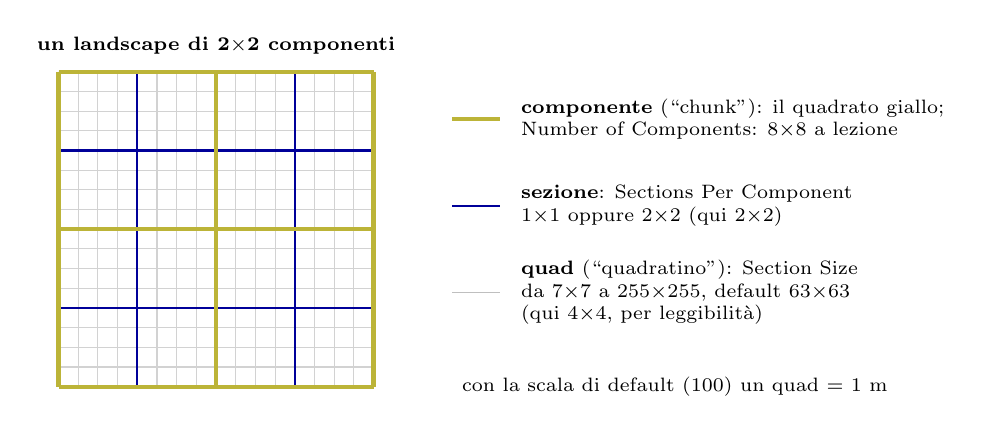
\begin{tikzpicture}[font=\footnotesize, x=1cm, y=1cm]
  % landscape 2x2 componenti, ognuno 2x2 sezioni, sezioni 4x4 quad (schematico)
  \begin{scope}
    \draw[gray!35, step=0.25] (0,0) grid (4,4);
    \draw[blue!60!black, thick, step=1] (0,0) grid (4,4);
    \draw[yellow!70!black, ultra thick, step=2] (0,0) grid (4,4);
    \node[anchor=south, font=\scriptsize\bfseries] at (2,4.1) {un landscape di 2$\times$2 componenti};
  \end{scope}
  % legenda
  \begin{scope}[xshift=5cm]
    \draw[yellow!70!black, ultra thick] (0,3.4) -- (0.6,3.4);
    \node[anchor=west, align=left, font=\scriptsize] at (0.75,3.4) {\textbf{componente} (``chunk''): il quadrato giallo;\\Number of Components: 8$\times$8 a lezione};
    \draw[blue!60!black, thick] (0,2.3) -- (0.6,2.3);
    \node[anchor=west, align=left, font=\scriptsize] at (0.75,2.3) {\textbf{sezione}: Sections Per Component\\1$\times$1 oppure 2$\times$2 (qui 2$\times$2)};
    \draw[gray!50] (0,1.2) -- (0.6,1.2);
    \node[anchor=west, align=left, font=\scriptsize] at (0.75,1.2) {\textbf{quad} (``quadratino''): Section Size\\da 7$\times$7 a 255$\times$255, default 63$\times$63\\(qui 4$\times$4, per leggibilità)};
    \node[anchor=west, align=left, font=\scriptsize] at (0,0.0) {con la scala di default (100) un quad = 1 m};
  \end{scope}
\end{tikzpicture}
\caption{La struttura di un landscape. I componenti (i \emph{chunk} gialli della preview)
sono le unità che il motore gestisce separatamente; ogni componente è diviso in una o
quattro sezioni; ogni sezione è una griglia di quad. Più quad significano curve più
morbide e più peso. Schema con valori ridotti per leggibilità.}
\label{ue14:fig:struttura}
\end{figure}

\begin{table}[htbp]
\centering
\small
\begin{tabular}{@{}p{4.2cm}p{3.0cm}p{6.8cm}@{}}
\toprule
\textbf{Parametro} & \textbf{A lezione} & \textbf{Che cosa decide} \\
\midrule
Section Size & 63$\times$63 (default); provati 31$\times$31 e 7$\times$7 & quanti quad ha
ogni sezione: più quad, terreno più morbido e più pesante \\
Sections Per Component & 2$\times$2, poi 1$\times$1 & in quante sezioni è diviso ogni
componente \\
Number of Components & 8$\times$8 & quanti componenti sulle X e sulle Y (landscape lungo,
largo, quadrato) \\
Overall Resolution & ricalcolata & il numero totale di vertici per lato (deriva dai valori
sopra) \\
Location, Rotation, Scale & invariati & la posizione e la dimensione del landscape; la scala
cambia la dimensione dei quad \\
Material & rimandato & il materiale con cui il landscape nasce \\
Fill World & non usato & crea un landscape grande quanto il mondo \\
Edit Layers & visti nella Manage & i livelli di modifica sovrapposti, bloccabili \\
\bottomrule
\end{tabular}
\caption{I parametri di creazione del landscape visti a lezione.}
\label{ue14:tab:creazione}
\end{table}

\paragraph{Approfondimento: i numeri del landscape di default.} Un quad, con la scala di
default (100 su X e Y), misura un metro: è comodo, perché la griglia del terreno coincide
con quella del pavimento della gym. La \emph{Overall Resolution} è il numero di vertici per
lato: con sezioni di 63 quad, una sezione per componente e 8 componenti per lato si hanno
$8 \times 63 + 1 = 505$ vertici, cioè un landscape di 504 metri per lato; con 2$\times$2
sezioni per componente il conto raddoppia ($8 \times 126 + 1 = 1009$). Le dimensioni
ammesse sono quelle della forma $2^n-1$ (7, 15, 31, 63, 127, 255) perché ogni livello di
LOD dimezza i quad di una sezione. Il componente è l'unità che il motore disegna, scarta e
semplifica: componenti più grandi significano meno oggetti da gestire ma un controllo più
grossolano. Epic consiglia di non esagerare con il numero di componenti (qualche migliaio
al massimo) e di scegliere le dimensioni fra quelle raccomandate nella documentazione. I
\emph{layer} della scheda Manage sono gli \textbf{Edit Layers}, attivi di default in
Unreal Engine~5: ogni layer conserva le proprie modifiche di scultura e di pittura, si può
bloccare, nascondere o cancellare senza toccare gli altri, come in un programma di grafica.
Funzionamento generale dell'engine.

% ---------------------------------------------------------------------
\section{Il pennello: falloff, strength, Alpha e Pattern}
\label{ue14:sec:pennello}

Lo strumento con cui si modifica il landscape ``è un cerchio, un pennello''. Cliccando, il
terreno si alza nel punto evidenziato: ``perché si alza? Perché siamo su \textbf{Sculpt} come
tool''. Prima degli strumenti, però, il docente spiega il pennello, che ``lascia anche
questa specie di immagine residua quando passa'' e ha una serie di parametri comuni a quasi
tutti gli strumenti (tabella~\ref{ue14:tab:pennello}).

\paragraph{Size, Falloff e Strength.}
\begin{itemize}
  \item la \textbf{grandezza} del pennello (\emph{Brush Size}), ``quindi effettivamente quanto è
        largo'';
  \item il \textbf{falloff}: ``è la distanza che c'è fra il primo cerchio e il secondo
        cerchio''. Il pennello ha due cerchi concentrici: dentro il primo l'effetto è pieno,
        fra il primo e il secondo sfuma. Con falloff \textbf{0} ``è tutto pieno'', e quando si
        alza qualcosa ``si alza tutto in blocco''; con falloff \textbf{1} ``si alza solo la
        punta e il resto è tutto quanto ammorbidito, è tutta sfumatura'';
  \item la \textbf{strength} (\emph{Tool Strength}), ``la forza del tool'': a 0,1 l'effetto si
        applica lentamente, a 1 molto più in fretta. ``È quanto forte viene applicato lo
        strumento.''
\end{itemize}

\paragraph{I quadratini e lo stretch del materiale.} ``Cosa stiamo vedendo con questi
quadratini a terra?'' La griglia disegnata sul landscape mostra ``il modo in cui sono
strutturati i poligoni'' e quindi, ``di conseguenza, in che modo verrà \textbf{stretchato il
materiale} quando ce l'andiamo a mettere sopra''. Il docente confronta tre zone
(figura~\ref{ue14:fig:stretch}): in piano ``il massimo della fedeltà, della risoluzione''; su
una salita morbida un materiale ``stretchato mediamente, ma rimane compatto''; su una parete
alzata con falloff zero un materiale che ``esplode'', perché il terreno non sale ``dritto per
dritto verticale'': c'è un quad che viene tirato in verticale ``per far sì che un lato sia
sul livello superiore, l'altro lato sul livello inferiore'', e lì il materiale ``sarà tutto
rovinato''.

\paragraph{Le forme del falloff.} Il \emph{Brush Falloff} ha quattro forme
(figura~\ref{ue14:fig:falloff}):
\begin{itemize}
  \item \textbf{Smooth}: ``il fall off è morbido'';
  \item \textbf{Linear} (``sharp linear''): ``non è morbido, ma è lineare, è geometrico'', una
        linea ``che dritta per dritta parte dalla base e arriva verso l'alto'';
  \item \textbf{Spherical}: ``un effetto più bombato'', ``una sorta di collinetta'' che poi
        ``spiove verso il basso'';
  \item \textbf{Tip}, ``il fall off convesso'', l'opposto dello spherical: la base è morbida e
        poi diventa lineare, con un effetto che ricorda ``le montagne dell'isola di Drum'' di
        \emph{One Piece} (``Drummond Island'' nella trascrizione: sono i \emph{Drum
        Rockies}, montagne a colonna).
\end{itemize}
``A seconda della situazione utilizzerete lo strumento più adatto'': linee morbide con lo
spherical, forme più aguzze con il tip.

\paragraph{I Brush Type.} ``Di base, il brush è un semplice \textbf{cerchio}''
(\emph{Circle}). Ma ci sono altri tipi:
\begin{itemize}
  \item l'\textbf{Alpha}: ``ora il nostro pennello non è più un cerchio, è una
        \textbf{texture}''. Si sceglie la texture dalla lista e ``funziona esattamente come
        avevamo fatto per i materiali: ci sono degli 0 e degli 1'': il pennello alza i bianchi
        e lascia a terra i neri. Con una texture di prova fatta di due quadrati bianchi e due
        neri si vede bene; il pennello \textbf{ruota} seguendo il movimento perché è attivo
        l'\emph{Auto Rotate}, che si può disattivare. L'uso tipico è con le texture di
        \textbf{noise}, che creano ``disturbo'': troppo, se esagerato, ma ``può esservi utile
        per andare a creare un effetto montagnoso, zigrinato, che dalla distanza può essere
        piacevole alla vista''. Qui si possono cambiare solo la grandezza e poco altro;
  \item il \textbf{canale} della texture (\emph{Texture Channel}), disponibile sia nell'Alpha
        sia nel Pattern. Il docente ripassa i canali, visti ``alla prima lezione che avevo
        fatto'': una texture ha i canali \textbf{RGB}, e i grafici li usano ``per mettere più di
        un'informazione all'interno della stessa texture'', come nelle mappe \textbf{ORM}
        (\emph{ambient occlusion} nel rosso, \emph{roughness} nel verde, \emph{metallic} nel
        blu). Il pennello può usare solo il rosso, solo il verde o solo il blu; con il noise
        ``saranno tutte uguali'';
  \item il \textbf{Pattern}: ``un portare all'estremo quello che faceva l'alfa''. La texture
        non è più ``messa su un quadrato'' ma proiettata sotto un pennello circolare, ``una
        fusione delle due precedenti'', e si può modificare: la \textbf{scala} (più piccola,
        ``molta più differenza nella costruzione''), la \textbf{rotazione}, le \textbf{U} e le
        \textbf{V}, ``quindi il \emph{panning}'', cioè lo scorrimento della texture.
        L'esempio: ``la faccia di Marte'', la collina che sembra un volto: con una texture a
        forma di faccia ``sembra che il terreno sia costruito in forma di faccia'';
  \item il \textbf{Component}, ``che io non ho mai usato, per essere onesto'': lavora
        direttamente sui componenti, per esempio per alzare un singolo chunk. Utile per
        dividere il landscape in due zone, ``una zona superiore e una zona inferiore'', che il
        giocatore dovrà collegare ``facendo X cose''.
\end{itemize}

\begin{figure}[htbp]
\centering
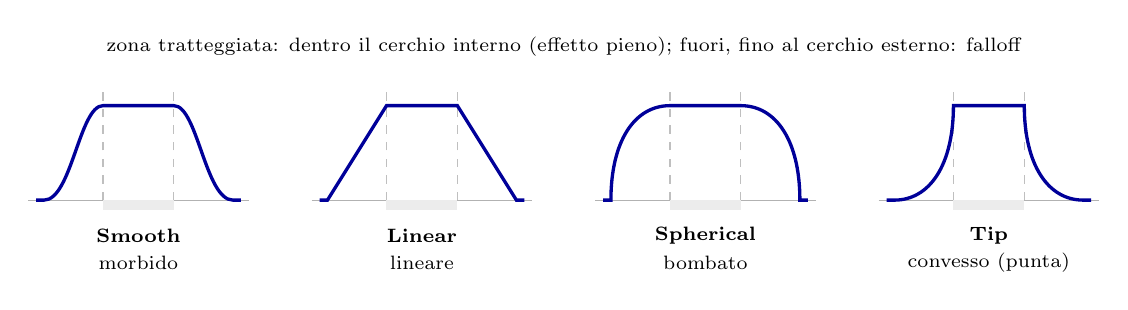
\begin{tikzpicture}[font=\footnotesize, x=1cm, y=1cm]
  \foreach \i/\name/\desc in {0/Smooth/morbido, 1/Linear/lineare, 2/Spherical/bombato, 3/Tip/convesso (punta)} {
    \begin{scope}[xshift=\i*3.6cm]
      \draw[gray!60] (-1.4,0) -- (1.4,0);
      \fill[gray!15] (-0.45,-0.12) rectangle (0.45,0);
      \draw[gray!50, dashed] (-0.45,0) -- (-0.45,1.4) (0.45,0) -- (0.45,1.4);
      \node[font=\scriptsize\bfseries] at (0,-0.45) {\name};
      \node[font=\scriptsize] at (0,-0.8) {\desc};
    \end{scope}
  }
  % Smooth: cosine
  \draw[very thick, blue!60!black] (-1.3,0) -- (-1.2,0) .. controls (-0.85,0) and (-0.75,1.2) .. (-0.45,1.2) -- (0.45,1.2) .. controls (0.75,1.2) and (0.85,0) .. (1.2,0) -- (1.3,0);
  % Linear
  \begin{scope}[xshift=3.6cm]
    \draw[very thick, blue!60!black] (-1.3,0) -- (-1.2,0) -- (-0.45,1.2) -- (0.45,1.2) -- (1.2,0) -- (1.3,0);
  \end{scope}
  % Spherical
  \begin{scope}[xshift=7.2cm]
    \draw[very thick, blue!60!black] (-1.3,0) -- (-1.2,0) .. controls (-1.2,0.75) and (-0.9,1.2) .. (-0.45,1.2) -- (0.45,1.2) .. controls (0.9,1.2) and (1.2,0.75) .. (1.2,0) -- (1.3,0);
  \end{scope}
  % Tip
  \begin{scope}[xshift=10.8cm]
    \draw[very thick, blue!60!black] (-1.3,0) -- (-1.2,0) .. controls (-0.75,0) and (-0.45,0.45) .. (-0.45,1.2) -- (0.45,1.2) .. controls (0.45,0.45) and (0.75,0) .. (1.2,0) -- (1.3,0);
  \end{scope}
  \node[font=\scriptsize, align=center] at (5.4,1.95) {zona tratteggiata: dentro il cerchio interno (effetto pieno); fuori, fino al cerchio esterno: falloff};
\end{tikzpicture}
\caption{Le quattro forme del \emph{Brush Falloff}, viste in sezione dopo aver alzato il
terreno con lo stesso pennello. Smooth sfuma in modo morbido, Linear con una rampa
dritta, Spherical con una collinetta bombata che spiove all'esterno, Tip con una base
morbida e una punta ripida. Profili schematici.}
\label{ue14:fig:falloff}
\end{figure}

\begin{figure}[htbp]
\centering
\begin{tikzpicture}[font=\footnotesize, x=1cm, y=1cm]
  % profilo del terreno con griglia di quad (vista laterale)
  \draw[gray!50] (0,0) -- (12,0);
  % piano
  \foreach \x in {0,0.5,...,3.5} {\draw[thick, green!40!black] (\x,0) -- (\x+0.5,0); \fill[green!40!black] (\x,0) circle (0.04);}
  \node[font=\scriptsize, align=center] at (2,-0.6) {piano: quad regolari\\``massima fedeltà''};
  % salita morbida
  \draw[thick, orange!80!black] (4,0) -- (4.5,0.15) -- (5,0.4) -- (5.5,0.7) -- (6,0.95) -- (6.5,1.1) -- (7,1.15);
  \foreach \p in {(4,0),(4.5,0.15),(5,0.4),(5.5,0.7),(6,0.95),(6.5,1.1),(7,1.15)} {\fill[orange!80!black] \p circle (0.04);}
  \node[font=\scriptsize, align=center] at (5.5,-0.6) {salita morbida:\\stretch medio};
  % parete
  \draw[thick, red!70!black] (7,1.15) -- (7.5,1.15) -- (8,1.15) -- (8.5,3.0) -- (9,3.0) -- (9.5,3.0);
  \foreach \p in {(7.5,1.15),(8,1.15),(8.5,3.0),(9,3.0),(9.5,3.0)} {\fill[red!70!black] \p circle (0.04);}
  \draw[red!70!black, thick] (8,1.15) -- (8.5,3.0);
  \node[font=\scriptsize, align=center, red!70!black] at (10.6,2.1) {un solo quad tirato\\in verticale: il\\materiale ``esplode''};
  \draw[-{Stealth[length=2mm]}, red!70!black] (9.7,2.1) -- (8.35,2.1);
  % texture schematica sopra la parete
  \foreach \t in {0.15,0.3,...,0.9} {\draw[red!40] ($(8,1.15)!\t!(8.5,3.0)$) -- ++(0.12,0);}
  \node[font=\scriptsize, align=center] at (8.5,-0.6) {parete con falloff 0:\\stretch estremo};
  % smooth
  \draw[-{Stealth[length=2mm]}, thick, blue!60!black] (10.4,1.0) -- (11.6,1.0);
  \node[font=\scriptsize, align=center, blue!60!black] at (11.0,0.35) {Smooth:\\quad più\\proporzionati};
\end{tikzpicture}
\caption{Lo \emph{stretch} del materiale, visto di lato. I punti sono i vertici della
griglia del landscape, a distanza fissa in pianta: in piano i quad sono regolari, su una
salita morbida si allungano un po', su una parete alzata in blocco un solo quad copre tutto
il dislivello e la texture si stira fino a diventare illeggibile. Lo strumento Smooth
riavvicina le proporzioni. Ricostruzione schematica.}
\label{ue14:fig:stretch}
\end{figure}

\begin{table}[htbp]
\centering
\small
\begin{tabular}{@{}p{3.6cm}p{10.4cm}@{}}
\toprule
\textbf{Parametro} & \textbf{Che cosa fa} \\
\midrule
Brush Size & la grandezza del pennello \\
Brush Falloff & la parte sfumata fra il cerchio interno e quello esterno: 0 tutto pieno, 1
tutto sfumato \\
Tool Strength & quanto in fretta e quanto forte si applica l'effetto (0,1 lento, 1 forte) \\
Falloff: Smooth, Linear, Spherical, Tip & la forma della sfumatura: morbida, lineare,
bombata, convessa a punta \\
Brush Type: Circle & il pennello circolare di base \\
Brush Type: Alpha & una texture come pennello: alza i bianchi, lascia i neri; Auto Rotate
lo fa ruotare con il movimento \\
Texture Channel & quale canale della texture usare (R, G o B) \\
Brush Type: Pattern & una texture proiettata sotto il pennello circolare, con scala,
rotazione e panning U/V \\
Brush Type: Component & agisce su interi componenti \\
\bottomrule
\end{tabular}
\caption{I parametri del pennello del Landscape Mode, comuni a quasi tutti gli
strumenti di scultura e di pittura.}
\label{ue14:tab:pennello}
\end{table}

\paragraph{Approfondimento: perché la parete ``esplode''.} Il landscape, essendo un
\emph{heightfield}, ha i vertici a distanza fissa in pianta: alzare un punto ne cambia solo
l'altezza, non la posizione orizzontale. Un dislivello di dieci metri fra due vertici
distanti un metro produce un quad lungo più di dieci metri e largo uno, e la texture,
mappata di default dall'alto (proiezione planare sul piano XY), vi si stira di dieci volte.
I rimedi sono tre: evitare pendenze troppo ripide (lo Smooth, che il docente chiama ``il
miglior amico dei vostri materiali''), usare nel materiale una proiezione che tenga conto
delle pareti (la proiezione \emph{triplanare} o \emph{world aligned}, che il materiale
StackOBot usa con la Absolute World Position), oppure coprire le pareti verticali con
delle mesh di roccia, come si fa quasi sempre nelle produzioni reali. Funzionamento
generale dell'engine.

% ---------------------------------------------------------------------
\section{La domanda sulle caverne}
\label{ue14:sec:caverne}

``C'è qualcosa che volevi chiedere per ora? Prima dicevi delle caverne che non si possono
fare.'' Uno studente ha provato a smanettare: è \textbf{impossibile fare dei buchi nel
landscape} con questi strumenti. Il docente conferma: ``per fare un buco avete bisogno dello
strumento \textbf{Visibility}, della \textbf{visibility mask}''. Ma la visibility mask ``si
modifica dal materiale del landscape'': bisogna aggiungere al materiale dei nodi specifici,
e solo allora si potrà avere una parte di landscape attraversabile, ``in cui possiamo andare
a costruire delle caverne''.

Lo studente pensava ad \textbf{Astroneer}, in cui scavare il terreno è la meccanica
principale. Il docente distingue due logiche: ``quando vai a creare un gioco devi far sì che
l'editor per il giocatore sia più \emph{user friendly} possibile''; ``quando stai creando un
editor, forse ti preoccupi di avere più possibilità possibili a disposizione''. Il buco ``si
può fare, non si può fare da qui''. In anteprima mostra lo strumento Visibility: il pennello
è \textbf{rosso} e cliccando non fa nulla, perché in basso Unreal avverte che il
\emph{visibility painting} è disabilitato: il componente ``non ha il nodo \textbf{Landscape
Visibility Mask} nel materiale''. Lo si vedrà a fine lezione
(sezione~\ref{ue14:sec:visibility}).

\paragraph{Approfondimento: terreni scavabili.} Giochi come Astroneer non usano un
heightfield ma un terreno \emph{volumetrico} (voxel), in cui ogni punto dello spazio sa se è
pieno o vuoto, e la superficie viene ricostruita a ogni modifica: per questo vi si possono
scavare tunnel e caverne in gioco. Il landscape di Unreal non funziona così, e una grotta
si fa nascondendo una porzione di terreno con la Visibility e costruendo l'interno con
delle mesh. Per terreni scavabili in Unreal esistono plugin di terzi basati sui voxel.
Funzionamento generale dell'engine.

% ---------------------------------------------------------------------
\section{Gli strumenti di scultura: Sculpt, Erase, Smooth, Flatten}
\label{ue14:sec:sculpt}

``Cosa fanno i nostri pennellozzi?'' ``Ognuno di voi troverà il modo con cui si trova più
comodo a fare le cose''; il docente mostra solo che cosa fa ogni strumento della scheda
\textbf{Sculpt} (tabella~\ref{ue14:tab:sculpt}).

\paragraph{Sculpt.} ``Il più semplice delle cose semplici'': scolpisce, alza il terreno. Ma,
come si è visto ``diverse volte per sbaglio'', non va solo verso l'alto: \textbf{Shift +
clic sinistro} ``scava'', e crea ``delle zone interrate'', delle depressioni.

\paragraph{Erase.} Cancella: ``elimina tutte le modifiche che abbiamo fatto, che siano verso
l'alto o verso il basso''. (Dopo la pausa il docente nota che anche l'Erase rispetta il
falloff: cancella ``in maniera sfumata'' le parti che cadono nella sfumatura.)

\paragraph{Smooth.} ``Ammorbidisce. Immaginatevelo come uno strumento che crea
sfumature.'' Se il pennello prende sia una parte alta sia una parte bassa, cliccando ``crea
una discesa più morbida'': ``fa una media, alza le parti abbassate, abbassa le parti un
pochino più alte'' e produce una \emph{slope} più leggera. ``Lo strumento Smooth è il miglior
amico dei vostri materiali'': ricordando che quanto sono stirati i quadratini ``è anche quanto
saranno stretchati i materiali'', uno smoothing li rende ``sempre più proporzionati''. Con un
pennello più grande della cima, però, ``lui abbassa proprio tutto''; per i ``lavori di fino''
si rimpicciolisce il pennello e si fanno piccole modifiche ``che non vanno a sbragare
completamente tutta la parete''. Anche qui ci sono falloff, tipi di pennello e strength, e
un parametro in più per la \textbf{precisione} dello smoothing (il \emph{Detail Smooth}):
``più grande è questo valore, più dettagli vengono rimossi'', più piccolo, ``meno dettagli
vengono rimossi''. I ``dettagli'' sono ``tutti questi su e giù'': con un valore alto e un
pennello grande ``lui pialla tutto'', con un valore piccolo i cambiamenti sono ``molto
morbidi'' e ``molto precisi''; ``a zero chiaramente non farà mai nulla''.

\paragraph{Flatten.} ``Il mio strumento preferito.'' Il docente si costruisce ``un piccolo
parco giochi'' di colline per gli esempi. Il \textbf{Flatten} ``ci permette di selezionare un
punto e appiattire tutto quanto a quell'altezza'': si clicca dove c'è la croce e tutto ciò
che passa sotto il pennello viene portato a quell'altezza, sia in basso sia sulla vetta.
Serve a una ``terraformazione un po' più controllata'':
\begin{itemize}
  \item \textbf{plateau}, altopiani: il ``lenzuolo'' tirato su si interrompe al bordo,
        ``non riscende giù'';
  \item \textbf{scaloni}, cliccando su punti diversi di una slope: ``scalone, altro scalone,
        altro scalone'', ``delle formazioni un po' più sensate, un po' più normali'', da
        ammorbidire poi con lo Smooth. Per esempio ``le cascatine fatte a livelli'' o ``le
        \textbf{risaie}'', con parti piatte e parti rialzate;
  \item un \textbf{canyon} dentro una parte rialzata: un fondo appiattito e i lati rimasti
        alti.
\end{itemize}

\paragraph{Le modalità del Flatten.} ``È abbastanza brutale come strumento, perché prende e
appiattisce tutto'': si rischia di appiattire le cose sbagliate. Per questo c'è la
\textbf{Flatten Mode} (figura~\ref{ue14:fig:flatten}):
\begin{itemize}
  \item \textbf{Both} (default): ``alza i piani che stanno più in basso e abbassa i piani che
        stanno più in alto'';
  \item \textbf{Raise}: alza tutti i punti fino all'altezza scelta, ``però non abbassa''.
        Esempio: un rilievo che fa da \textbf{bordo della mappa} resta intatto, e si alza
        solo ciò che c'è sotto;
  \item \textbf{Lower}: abbassa ``tutto quello che c'è da abbassare, ma non alza'': ``se c'è
        una grotta o un canyon che deve rimanere giù, non lo tira più su''.
\end{itemize}
``Principalmente questi sono i due che vorrete utilizzare, perché sono quelli che vi danno
un po' più di controllo.'' Di un'altra opzione il docente legge a fatica il nome (``height
intervals'', ``specification at intervals''): ``questo è uno che effettivamente non ho mai
utilizzato''. Si tratta, con ogni probabilità, della modalità \textbf{Terrace} (si veda
l'approfondimento).

\paragraph{Use Slope Flatten.} Con la casella \textbf{Use Slope Flatten}, invece di
appiattire in orizzontale ``andate a continuare il piano diagonale preso originariamente'':
cliccando su un pendio, lo strumento prolunga quella pendenza, ``anche scavando verso il
basso''. Serve per ``quei pianori, quegli spiazzi montani'' che sono ``uno spaccato dritto per
dritto, che però va in diagonale''. Ultimo uso, personale: ``a volte il Flatten tendo a
utilizzarlo tipo \textbf{gomma}'': si punta sul livello base del landscape e si appiattisce.

``Abbiamo visto scolpire, tirare su, tirare giù, ammorbidire, cancellare e appiattire.''

\begin{figure}[htbp]
\centering
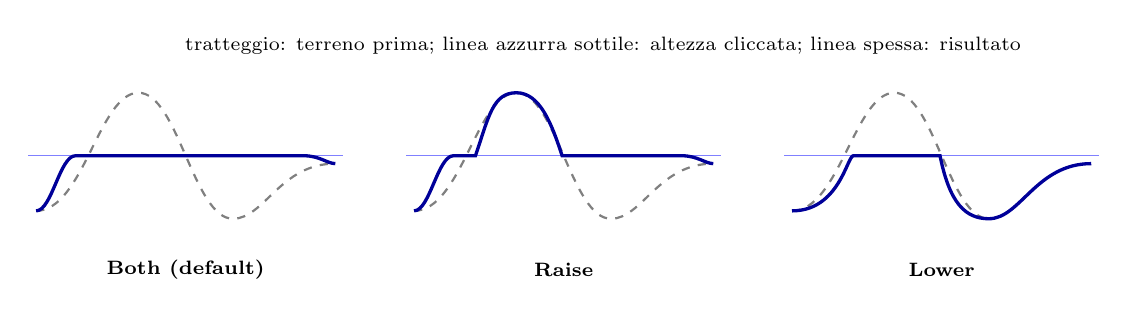
\begin{tikzpicture}[font=\footnotesize, x=1cm, y=1cm]
  \foreach \i/\name in {0/Both (default), 1/Raise, 2/Lower} {
    \begin{scope}[xshift=\i*4.8cm]
      % profilo originale
      \draw[gray, dashed, thick] (0,0.3) .. controls (0.6,0.3) and (0.8,1.8) .. (1.3,1.8) .. controls (1.8,1.8) and (2.0,0.2) .. (2.5,0.2) .. controls (2.9,0.2) and (3.1,0.9) .. (3.8,0.9);
      \draw[blue!50, thin] (-0.1,1.0) -- (3.9,1.0);
      \node[font=\scriptsize, blue!60!black, anchor=west] at (3.9,1.0) {};
      \node[font=\scriptsize\bfseries] at (1.9,-0.45) {\name};
    \end{scope}
  }
  % Both: tutto a 1.0
  \draw[very thick, blue!60!black] (0,0.3) .. controls (0.2,0.3) and (0.3,1.0) .. (0.5,1.0) -- (3.4,1.0) .. controls (3.6,1.0) and (3.7,0.9) .. (3.8,0.9);
  % Raise: alza le valli, non abbassa la cima
  \begin{scope}[xshift=4.8cm]
    \draw[very thick, blue!60!black] (0,0.3) .. controls (0.2,0.3) and (0.3,1.0) .. (0.5,1.0) -- (0.78,1.0) .. controls (0.95,1.5) and (1.0,1.8) .. (1.3,1.8) .. controls (1.6,1.8) and (1.75,1.4) .. (1.88,1.0) -- (3.4,1.0) .. controls (3.6,1.0) and (3.7,0.9) .. (3.8,0.9);
  \end{scope}
  % Lower: abbassa la cima, non alza le valli
  \begin{scope}[xshift=9.6cm]
    \draw[very thick, blue!60!black] (0,0.3) .. controls (0.6,0.3) and (0.7,1.0) .. (0.78,1.0) -- (1.88,1.0) .. controls (2.0,0.4) and (2.2,0.2) .. (2.5,0.2) .. controls (2.9,0.2) and (3.1,0.9) .. (3.8,0.9);
  \end{scope}
  \node[font=\scriptsize, align=center] at (7.2,2.4) {tratteggio: terreno prima; linea azzurra sottile: altezza cliccata; linea spessa: risultato};
\end{tikzpicture}
\caption{Le tre modalità principali del Flatten, in sezione. Both porta tutto all'altezza
cliccata; Raise alza solo ciò che sta sotto e lascia la cima (per esempio il bordo della
mappa); Lower abbassa solo ciò che sta sopra e lascia le valli (per esempio un canyon).
Profili schematici.}
\label{ue14:fig:flatten}
\end{figure}

\paragraph{Approfondimento: Terrace e gli altri parametri del Flatten.} Nella versione di
Unreal Engine~5 il Flatten ha quattro modalità: oltre a Both, Raise e Lower, la modalità
\textbf{Terrace}, che appiattisce il terreno a \emph{intervalli} di altezza regolari
(\emph{Terrace Interval}), con una sfumatura fra un gradino e l'altro (\emph{Terrace
Smooth}): è lo strumento giusto per le risaie e le cascate a livelli che il docente
costruisce a mano cliccando su più punti. Altri parametri utili: \emph{Pick Value Per
Apply}, che ricampiona l'altezza a ogni pennellata invece di tenere quella del primo clic;
\emph{Flatten Target}, che permette di scrivere a mano l'altezza a cui appiattire (comodo
per avere esattamente le misure della gym, per esempio un plateau a 1,40 m sopra un
altro); e \emph{Show Preview Grid}, che mostra il piano di destinazione. Funzionamento
generale dell'engine; la lezione non li tocca.

% ---------------------------------------------------------------------
\section{Ramp e i LOD}
\label{ue14:sec:ramp}

``Adesso vediamo uno strumento che funziona in maniera un po' diversa. Non è più un
pennello, ma dei clic'': lo strumento \textbf{Ramp}. Si clicca su due punti, li si sposta
come si vuole, e quando si è contenti si preme \textbf{Add Ramp}: Unreal aggiunge ``un
collegamento di landscape da punto A a punto B''. Il docente chiede alla classe che cosa
succederà con due punti sul fondo di due valli separate da una collina: ``ti farà un canyon
lì in mezzo'' (la rampa porta il terreno ``sempre da punto A a punto B'', anche scavando).

\paragraph{Gli usi.}
\begin{itemize}
  \item una \textbf{rampa} per salire su un punto sopraelevato (``sarà un modo molto brutto,
        però va'');
  \item le rampe di un gioco di \textbf{macchine} o di \textbf{skateboard};
  \item ``una \textbf{diga} in un crepaccio'', un collegamento pieno da una parte all'altra.
\end{itemize}
Un \textbf{ponte sospeso}, invece, no. Si potrebbe pensare di fare la diga e poi bucarla
sotto con la Visibility, ``tuttavia ci sarebbe un problema'': la parte sotto non
collegherebbe più le due metà, ``perché il landscape \textbf{non può essere sovrapposto}'',
``non può esserci una parte qui e una parte sotto''. ``Se volete fare un ponte sospeso,
fatelo con le \textbf{mesh}: prendete una mesh, ingranditela e mettetela sopra un crepaccio.
Non fatelo con il landscape.''

\paragraph{Larghezza e falloff.} La rampa ha la sua \textbf{larghezza} (\emph{Ramp Width}),
``se un ponticello, se una grossa salita'', e il suo \textbf{falloff} (\emph{Side Falloff}):
a zero non c'è sfumatura e i lati vengono stirati ``a blocco''; tutto sfumatura, e il
terreno attorno si raccorda morbido. Ma se si ``tira la corda'', con molta sfumatura e una
rampa molto stretta, ``vi si spacca un po' il landscape'': ``questa cosa è molto rotta, e
dalla distanza sarà tremenda'', ``perché i \textbf{LOD} vanno a semplificare il landscape''.

\paragraph{I LOD.} ``Sapete che cos'è un LOD?'' \textbf{LOD} sta per \emph{Level of Detail}.
Un grafico crea una mesh, poniamo da 10.000 poligoni; questa mesh deve avere ``altre
versioni di sé più grezze'', da 5.000, da 2.000 poligoni, perché l'engine, ``e non solo in
automatico'', aggiorna il numero di poligoni ``a seconda della distanza da cui lo vedi''.
L'esempio della statua: da vicino deve essere ``super bellissima'', ma da lontano ``non serve
che abbia ancora 500.000 poligoni'', perché l'occhio non vedrà il dettaglio, e ridurli
alleggerisce le prestazioni. Le distanze si possono impostare (``a 10 metri un tot, a 20
metri un altro tot, a 40 metri un altro tot''), da un Blueprint o dalla mesh stessa. Il
landscape funziona allo stesso modo: dalla distanza i suoi poligoni vengono semplificati.
Una massa grande non ne soffre, ``perché ci sono molti poligoni''; una rampa sottilissima,
``costituita di troppi pochi poligoni, viene distrutta dai LOD''. ``Quindi evitate di fare
delle robe in questo modo.''

\paragraph{Lo sfogo sui Pokémon.} L'esempio, dichiaratamente polemico: i recenti Pokémon
open world, \emph{Scarlatto e Violetto} e \emph{Leggende Pokémon: Arceus}. ``Potete vedere
attivamente la terra che si muove, come se fosse animata'': ``sono semplicemente i LOD che si
attivano troppo presto'', il landscape ``viene semplificato con troppo anticipo''. Il
motivo, secondo il docente, è l'ottimizzazione: se in una visione ampia si vedesse tutto
con tutti i poligoni ``esploderebbe la console''. ``Non è che sono brutte, ma è che sono
troppo ottimizzate, e la troppa ottimizzazione le rende orribili''; e sono così ottimizzate
``perché il gioco è programmato in maniera talmente stupida da essere pesante''. ``Scusate
questo piccolo sfogo contro Game Freak.'' (È un giudizio personale del docente, non
un'analisi tecnica verificata; il fenomeno del terreno che ``si muove'' quando cambia il LOD,
il \emph{LOD popping}, è comunque reale e ben noto.)

\paragraph{La regola.} ``Diamo sempre un po' di spazio al landscape'': niente forme troppo
sottili. ``Questo è anche il motivo per cui vorremmo evitare dei landscape troppo piccoli'':
un landscape 7x7 ``capita molto spesso che si spacchi in questo modo, perché ha pochi
poligoni a disposizione''. Il docente rifà ``una rampina decente''.

\paragraph{Approfondimento: i LOD del landscape.} Il landscape non ha LOD costruiti a mano
come una static mesh: li calcola da solo, dimezzando a ogni livello i quad di ogni sezione
(per questo le Section Size sono della forma $2^n-1$). La transizione è regolata da
parametri dell'actor Landscape (in Unreal Engine~5 \emph{LOD 0 Screen Size}, \emph{LOD 0
Distribution Setting} e \emph{LOD Distribution Setting}, più eventuali \emph{LOD Group}),
che decidono a quale dimensione sullo schermo un componente passa al livello successivo.
Aumentarli rende il terreno lontano più fedele e più costoso. Le forme più sottili di una
sezione, come la rampa stretta del docente, sono le prime a sparire perché nel livello
semplificato non ci sono più vertici abbastanza vicini per descriverle. Il capitolo 12 di
Romero e Sewell, sulla pubblicazione, ricorda che fra le impostazioni di scalabilità del
gioco c'è anche la qualità del \emph{foliage}, e che se le prestazioni calano solo in certe
zone del livello conviene ``ridurre la densità degli oggetti'' o la qualità di un modello:
il compromesso fra dettaglio e prestazioni di cui parla il docente. Per la parte sui
parametri del landscape, funzionamento generale dell'engine.

% ---------------------------------------------------------------------
\section{Erosion, Hydro, Noise, Mirror e Copy/Paste}
\label{ue14:sec:altristrumenti}

\paragraph{Erosion e Hydro.} ``Sono due strumenti con cui io faccio un po' a botte'' (``a
volte'' nella trascrizione, ma il seguito chiarisce il senso): il
docente spiega a che cosa servirebbero e perché non gli piacciono. L'idea è ``simulare
delle deformazioni, del \emph{displacement}''. L'\textbf{Erosion} è lo strumento con cui
``andrei a dettagliare una parete montuosa'': ``è un po' il contrario dello smooth'', crea
nel pennello parti rialzate e parti abbassate. (Qui la trascrizione si interrompe in una
frase ripetuta; riprende con la domanda di uno studente.)
\begin{itemize}
  \item il \textbf{Threshold} ``va a definire quanta differenza fra punto A e punto B deve
        esserci per andare a fare erosione'': con un valore alto l'erosione si applica solo
        dove il dislivello è grande; abbassandolo (``tipo 17'') si erode ``molto di più, in
        molti punti diversi'', perché basta una differenza minore;
  \item \textbf{Noise Mode} e \textbf{Noise Scale} aggiungono un rumore preimpostato, e come
        nel Flatten si sceglie se deve alzare e abbassare, solo alzare o solo abbassare.
\end{itemize}
L'\textbf{Hydro} (\emph{Hydro Erosion}) ``funziona più o meno nello stesso modo'' e
vorrebbe creare un \emph{displacement} ``stile fondali marini'' o ``erosione dell'acqua''. Il
problema è che ``abbiamo un po' poco controllo'': ``io non sono mai riuscito a farlo
funzionare bene, proprio non mi trovo''.

\paragraph{Noise.} ``Preferisco piuttosto utilizzare il \textbf{Noise}'', che ``fa rumore'' e
permette di scegliere se aggiunge, se toglie o se fa entrambe le cose. Con un pennello
grande e la scala del noise ridotta, ``vi va a fare una deformazione un po' più subdola'':
``non prende e spacca, ma fa dei leggeri movimenti di alzare e abbassare'', il risultato
``che al mio occhio è sempre il più piacevole''. In modalità solo-aggiunta il Noise alza,
``però non come lo Sculpt'' (aggiunge rumore, non una collina); lo stesso vale per la
sottrazione.

\paragraph{Gli strumenti saltati.} ``Facciamo al volissimo le ultime cose'':
\begin{itemize}
  \item il \textbf{Retopologize} ``non ci interessa'';
  \item la \textbf{Visibility}, già vista, si riprende più avanti;
  \item il \textbf{Blueprint Brush}, ``qualcosa che onestamente non ho mai utilizzato'':
        ``presumo sia un brush che può essere programmato'' per fare cose specifiche. ``Non
        l'ho mai trovato necessario.''
\end{itemize}

\paragraph{Mirror.} Il \textbf{Mirror} serve ``nel momento in cui avete degli ambienti molto
grandi che volete copiare, che volete specchiare o che volete ruotare''. Compare un
\textbf{piano}: premendo \textbf{Apply}, tutto ciò che sta da un lato viene copiato
sull'altro, ``appiattendo'' quello che c'era. Il piano si sposta avanti e indietro, e
soprattutto dall'\textbf{Operation} si sceglie il tipo di operazione:
\begin{itemize}
  \item \textbf{-X to +X}: copia il lato sinistro sul destro; \textbf{+X to -X} il contrario;
        lo stesso per \textbf{-Y to +Y} e \textbf{+Y to -Y}. Con una forma qualsiasi si ottiene
        ``una macchia di Rorschach'';
  \item le varianti \textbf{Rotate} (per esempio \emph{Rotate -X to +X}): stessa direzione del
        piano, ``ma operazione diversa'': invece di specchiare, ruota, ``come se prendesse
        questa parte del landscape e la ruotasse nell'altra direzione''. Il risultato è
        uguale, ``ma ruotato''.
\end{itemize}

\paragraph{Copy/Paste.} ``Il copia e incolla, la cosa più semplice del mondo.'' Prima si
seleziona una parte di landscape con lo strumento \textbf{Region Select} (``Select''),
dipingendo la zona con il pennello; per togliere la selezione serve \textbf{Clear Region
Selection}, ``perché se andate da altre parti questo vi rimane sempre selezionato''. Poi,
nello strumento \textbf{Copy/Paste}, \textbf{Ctrl+C} copia la zona in un riquadro (il
\emph{gizmo}) che si può spostare, ruotare e scalare dove si vuole, e \textbf{Ctrl+V} la
incolla, ``modificata, ruotata e anche scalata''. Ci sono comandi per adattare il riquadro
alla selezione e per ripulirlo. La \textbf{Paste Mode} ripete la logica del Flatten:
\begin{itemize}
  \item \textbf{Both}: tutto il riquadro viene portato al livello copiato, la zona di
        destinazione viene abbassata a livello base e la parte copiata rialzata;
  \item \textbf{Raise}: alza soltanto ``le parti che erano più basse'' e non abbassa le altre:
        di una collina copiata sopra un'altra resta solo ``la punta'';
  \item \textbf{Lower}: l'opposto.
\end{itemize}
``Abbiamo effettivamente un po' tutte le cose viste.'' Nessuna domanda: pausa, ``ci becchiamo
alle 55 con il Paint, e quindi i materiali del landscape''.

\begin{table}[htbp]
\centering
\small
\begin{tabular}{@{}p{3.0cm}p{11.0cm}@{}}
\toprule
\textbf{Strumento (Sculpt)} & \textbf{Che cosa fa, e come lo usa il docente} \\
\midrule
Sculpt & alza il terreno; Shift + clic scava \\
Erase & cancella le modifiche (rispetta il falloff) \\
Smooth & fa una media delle altezze; Detail Smooth decide quanto dettaglio togliere; ``il
miglior amico dei materiali'' \\
Flatten & appiattisce all'altezza cliccata; Flatten Mode Both, Raise, Lower (e Terrace);
Use Slope Flatten prolunga il pendio; usato anche come ``gomma'' \\
Ramp & crea una rampa fra due punti (Add Ramp), con Ramp Width e Side Falloff; non per i
ponti sospesi \\
Erosion & dettaglia le pareti erodendo dove il dislivello supera il Threshold; Noise Mode e
Noise Scale; ``poco controllo'' \\
Hydro (Hydro Erosion) & erosione ``ad acqua''; il docente non lo usa \\
Noise & aggiunge o toglie rumore; con scala piccola, deformazioni ``subdole'' \\
Retopologize & non visto (``non ci interessa'') \\
Visibility & nasconde porzioni di terreno; richiede la Landscape Visibility Mask nel
materiale \\
Blueprint Brush & pennelli programmabili; mai usato dal docente \\
Mirror & specchia (-X to +X, \dots) o ruota (Rotate \dots) metà del landscape; Apply \\
Region Select & seleziona una zona col pennello; Clear Region Selection \\
Copy/Paste & Ctrl+C e Ctrl+V di una zona, con gizmo spostabile, ruotabile, scalabile;
Paste Mode Both, Raise, Lower \\
\bottomrule
\end{tabular}
\caption{Gli strumenti della scheda Sculpt del Landscape Mode, nell'ordine della lezione.}
\label{ue14:tab:sculpt}
\end{table}

\paragraph{Approfondimento: il terreno come spazio di gioco.} Gli strumenti di scultura
sono tecnici, ma le forme che producono sono categorie di level design. Totten, nel
capitolo 3, osserva che in un open world fatto di paesaggi aperti, come \emph{Skyrim}, i
percorsi fra città e dungeon ``sono molto meno diretti'' e spesso ``campi aperti'': il
giocatore traccia da sé le scorciatoie fra i landmark, ma ``rischia di perdersi'', e i
designer usano ``elementi geografici sottili come sentieri sterrati, cartelli o fiumi'' per
suggerire i percorsi. E aggiunge proprio a proposito degli ``editor di terreno integrati
nell'engine'': tenere a mente queste linee guida serve a creare mondi ``non solo
esteticamente attraenti, ma anche utilizzabili''. Il canyon del Flatten, la diga della Ramp
e il bordo di mappa preservato dal Raise sono, in questi termini, un percorso, un
collegamento e un \emph{edge}; il plateau è un'area in cui il giocatore guarda lontano (il
\emph{prospect space} dello stesso capitolo). Le misure, infine, vengono dalla gym: un
canyon che deve essere invalicabile avrà pareti oltre il Walkable Floor Angle del
personaggio, un plateau raggiungibile con un salto starà sotto l'altezza comoda misurata.

% ---------------------------------------------------------------------
\section{La pausa e la domanda su The Sims}
\label{ue14:sec:pausa}

Alla ripresa (``Guido c'è, Federico c'è, Giulia c'è'') il docente chiede se sia tutto
chiaro: ``è abbastanza semplice, è più una questione di prenderci la mano''. Consiglia di
usare il landscape ``fra questa lezione e la prossima'' per familiarizzare e trovare il
proprio modo di lavorare: ``magari siete dei pazzi completi e lavorate utilizzando soltanto
lo Sculpt, ma siete fortissimi. Io vi dico quali sono i tool, poi voi trovate il vostro
modo di lavoro''.

\paragraph{The Sims.} Uno studente chiede se il terreno della serie \textbf{The Sims}, ``soprattutto
del 2'', sia fatto allo stesso modo. Il docente non lo sa: ``non so con cosa è stato fatto''.
Dopo un rapido controllo: ``a quanto risulta, ogni The Sims ha usato un \textbf{engine custom}''.
È ``plausibile'' che funzioni in modo simile, e che ci sia stata ``una \emph{cross
contamination}, delle influenze da entrambe le parti'': magari anche Unreal si è ispirato a
come ``diversi tycoon o diversi simulatori'' gestivano la terraformazione, perché ``quel tipo
di modifica spaziale è molto comodo farla con un pennello''. ``Non ti so dire di più'':
l'ultima volta che ha giocato a The Sims ``probabilmente era vent'anni fa''. Lo invita a fare
una ricerca e a riferire la volta successiva. (Nello scambio, alla domanda ``quando è uscito
The Sims 2?'', la risposta è ``nel 2000'': in realtà nel 2000 è uscito il primo
\emph{The Sims}; \emph{The Sims 2} è del 2004.)

% ---------------------------------------------------------------------
\section{Il Paint e il materiale del landscape di StackOBot}
\label{ue14:sec:paint}

``Abbiamo visto il Manage, abbiamo visto lo Sculpt, rimane soltanto da vedere il
\textbf{Paint}.'' La scheda ha ``più o meno gli stessi strumenti che c'erano di là'':
\textbf{Paint}, \textbf{Smooth}, \textbf{Flatten} e \textbf{Noise}, con la stessa strength e
gli stessi tipi di pennello. Ma in basso Unreal avverte: \emph{non ci sono target layer
assegnati a questo landscape; usa i bottoni in alto per aggiungerne di nuovi o popolarli
dal materiale correntemente assegnato}. I bottoni sono \textbf{Create Layer} e
\textbf{Create Layers from Assigned Materials}, quest'ultimo, ``se non sbaglio, unico di
Unreal 5, sulla quarta edizione non c'è''.

\paragraph{Un materiale normale non basta.} Il landscape può \textbf{dipingere il materiale}
con il pennello, ``il materiale però deve essere fatto \emph{ad hoc}''. Prova: un nuovo
materiale con dentro ``unicamente un colore''. Messo sul landscape, il landscape lo tratta
``come un oggetto qualsiasi'': ``tutto quanto diventa disgustosamente verde'', e non c'è modo
di modificare nulla, ``perché il nostro materiale di layer non ne ha''.

\paragraph{Il ``grosso errore''.} A questo punto il docente si accorge di ``aver fatto un grosso
errore: niente di grave, semplicemente una cosa che ci farà perdere un po' di tempo'' (la
spiegherà più avanti: sono le Virtual Texture, sezione~\ref{ue14:sec:grass}).

\paragraph{Il pacchetto StackOBot.} Fra gli asset del pacchetto \textbf{StackOBot}, ``il
pacchettino con il robottino e tutte le cose'', nella cartella \emph{Environment} ci sono:
\emph{Props} e \emph{Modular} (mesh da vedere alla fine della lezione ``o all'inizio della
prossima''), \emph{Materials}, \emph{Foliage} (per il Foliage Mode) e \textbf{Landscape}, con
``tutto quello che riguarda il landscape'': delle texture ``che non sappiamo bene cosa
fanno'', una mesh che per ora non serve, dei materiali, fra cui \textbf{M\_Landscape}, e dei
\textbf{Landscape Layers} ``che non sappiamo bene cosa fanno'' e che si rivedranno più
tardi.

\paragraph{Il nero.} Si assegna M\_Landscape al landscape (nel campo \emph{Landscape
Material} dei Details): ``va tutto \textbf{nero}''. Anche un materiale pensato per il
landscape, appena assegnato, ``non ci dà subito quello di cui abbiamo bisogno''; e ``il fatto
che diventi tutto nero è quello che vogliamo, per noi è positivo''. Bisogna stabilire come
funzionano i layer: visto che il materiale ``è già stato costruito per avere tanti layer
diversi'', si preme \textbf{Create Layers from Assigned Materials}. Unreal crea
\textbf{quattro layer}, e il terreno resta nero. (Resta nero perché nessun layer è ancora
stato dipinto: si veda l'approfondimento.)

\paragraph{Dentro M\_Landscape.} Il docente apre il materiale, ``molto piccolo, vero?
Molto comodo'' (ironico: il nodo principale è ridotto a un solo pin). Le parti interessanti:
\begin{itemize}
  \item quattro \textbf{material function}, \emph{MF\_Rocks}, \emph{MF\_Pebbles},
        \emph{MF\_Sand} e \emph{MF\_Grass}: ``il funzionamento dei singoli materiali, quindi
        dei singoli layer''. Si creano con tasto destro, \emph{Material Function}: sono
        ``delle piccole funzioni'', come quelle dei Blueprint, che descrivono ``come funziona
        l'erba, come funziona la ghiaia, i \emph{pebbles}'', la roccia e la sabbia;
  \item dentro ogni funzione le texture sono collegate alla \textbf{Absolute World
        Position}: ``vi ricordate i materiali \textbf{world aligned} che avevamo visto la
        volta scorsa? Questo è il modo per farli, anche per il landscape'';
  \item tutte le funzioni terminano con un nodo \textbf{Set Material Attributes}: un nodo
        ``vuoto'' in cui, aggiungendo slot all'array, si decide quale informazione passa ogni
        ingresso (Base Color, Metallic, Specular, Roughness, Normal\dots). Qui ogni funzione
        passa \textbf{Base Color}, \textbf{Roughness} e \textbf{Normal} del proprio materiale,
        presi da dei \emph{Texture Sample} (``vi ricordate, l'abbiamo fatta questa roba'');
  \item le quattro uscite entrano nel nodo che è ``alla base del funzionamento del
        materiale del landscape'': il \textbf{Landscape Layer Blend}.
\end{itemize}

\paragraph{I nodi del landscape.} Cercando \emph{landscape} nella palette dei nodi, Unreal
mostra ``tutti i nodi che sono utili per il landscape''. Oggi se ne vedono tre (più uno ``che
sta da un'altra parte'', il Landscape Grass Output): il \textbf{Landscape Layer Blend},
``il fondamentale'', il \textbf{Landscape Layer Sample} e la \textbf{Landscape Visibility
Mask}.

\paragraph{Landscape Layer Blend.} È un nodo ``vuoto'', come il Set Material Attributes, in
cui si aggiungono elementi all'array \emph{Layers}. Ogni elemento si apre con delle
freccette, e lì si scrive il \textbf{nome del layer} (per esempio \emph{Grass}).
``Scriveteli bene, perché è importante scrivere bene il nome del layer'': se non c'è il
nome, ``Unreal non lo trova, non lo rileva'', anche se ci sono collegate delle cose; e altri
nodi, come il Landscape Layer Sample, ``hanno bisogno del nome per funzionare''. Gli altri
campi dell'elemento ``sono dei parametri di preview che al momento non ci interessano''.
Usando questo nodo, gli autori del materiale hanno fatto quattro layer: \textbf{roccia},
\textbf{sassolini} (ghiaia), \textbf{sabbia} ed \textbf{erba}, tutti collegati al nodo
risultante del materiale.

\paragraph{Use Material Attributes.} Il nodo risultante è ``così piccolino'' perché nei
dettagli del materiale è spuntata la casella \textbf{Use Material Attributes}, che
``trasforma il modo in cui funziona il nodo'': invece di avere un pin per Base Color, uno per
Roughness, uno per Normal, ha un unico ingresso \emph{Material Attributes}. Senza la casella
bisognerebbe collegare il risultato su ogni parametro, cosa comoda se si vogliono
modificare le singole cose; ma poiché tutte le operazioni avvengono nelle funzioni, ``per
lui è comodo'' far passare tutto in un colpo solo.

\paragraph{Dipingere.} Che cosa permette la suddivisione in layer? ``Di avere dei layer da
poter dipingere.'' Selezionato \textbf{Rock} e passato il pennello, il terreno ``dipinge
roccia'', ``o perlomeno quello che noi abbiamo impostato come valore per il materiale della
roccia'': se non piace, la texture e le dimensioni si cambiano da dentro la sua material
function, ``tutto come abbiamo visto la volta scorsa''. Poi i \textbf{Pebbles} (``dei
sassolini, una ghiaietta''), la \textbf{Sand} e la \textbf{Grass}. Ogni volta Unreal deve
``compilare gli shader'', e ci vuole un po'.

\begin{figure}[htbp]
\centering
\begin{tikzpicture}[font=\scriptsize, x=1cm, y=1cm,
  ue14node/.style={draw, thick, rounded corners=2pt, fill=white, align=center, minimum height=0.6cm, inner sep=3pt},
  ue14fn/.style={ue14node, fill=yellow!15},
  ue14out/.style={ue14node, fill=gray!25, minimum width=2.6cm},
  ue14arr/.style={-{Stealth[length=1.6mm]}, thick}]
  \node[ue14fn] (r) at (0,3.0) {MF\_Rocks};
  \node[ue14fn] (p) at (0,2.2) {MF\_Pebbles};
  \node[ue14fn] (s) at (0,1.4) {MF\_Sand};
  \node[ue14fn] (g) at (0,0.6) {MF\_Grass};
  \node[font=\scriptsize, align=center] at (0,3.9) {material function:\\Texture Sample (World Position)\\$\rightarrow$ Set Material Attributes};
  \node[ue14node, minimum height=3.0cm, minimum width=2.8cm] (lb) at (4.2,1.8) {};
  \node[font=\scriptsize\bfseries] at (4.2,3.55) {Landscape Layer Blend};
  \foreach \n/\y in {Rock/2.6,Pebbles/2.0,Sand/1.4,Grass/0.8} {\node[font=\scriptsize, anchor=west] at (3.0,\y) {Layer \n};}
  \draw[ue14arr] (r.east) -- (3.0,2.6);
  \draw[ue14arr] (p.east) -- (3.0,2.0);
  \draw[ue14arr] (s.east) -- (3.0,1.4);
  \draw[ue14arr] (g.east) -- (3.0,0.8);
  \node[ue14out] (m) at (8.6,1.8) {M\_Landscape\\(Use Material Attributes)\\\emph{Material Attributes}};
  \draw[ue14arr] (lb.east) -- (m.west);
  % grass spawn
  \node[ue14node, fill=green!12] (ls) at (0.6,-1.2) {Landscape Layer Sample\\\emph{Parameter Name: Grass}};
  \node[ue14node] (calc) at (4.2,-1.2) {calcoli\\(GPU Grass Spawn)};
  \node[ue14out, fill=green!25] (go) at (8.6,-1.2) {Landscape Grass Output\\\emph{Grass: GT\_Grass}};
  \draw[ue14arr] (ls.east) -- (calc.west);
  \draw[ue14arr] (calc.east) -- (go.west);
  \node[ue14node, fill=blue!8] (gt) at (8.6,-2.6) {Landscape Grass Type: mesh,\\densità, scala min--max};
  \draw[ue14arr, dashed] (gt.north) -- (go.south);
  \node[font=\scriptsize, align=left, anchor=west] at (-1.4,-2.6) {i nomi \emph{Grass} devono coincidere\\esattamente (maiuscole comprese)};
\end{tikzpicture}
\caption{Lo schema del materiale M\_Landscape di StackOBot come descritto a lezione. In
alto, la parte che \emph{dipinge}: quattro material function entrano nel Landscape Layer
Blend, ognuna nel layer con il proprio nome, e il risultato va al nodo del materiale con
Use Material Attributes. In basso, la parte separata che \emph{fa spawnare} l'erba: un
Landscape Layer Sample legge dove è stato dipinto il layer Grass e, dopo alcuni calcoli,
alimenta il Landscape Grass Output, che usa un Landscape Grass Type. I nodi grigi sono
nodi finali. Ricostruzione schematica.}
\label{ue14:fig:materiale}
\end{figure}

\paragraph{Approfondimento: perché il terreno è nero, e i pesi dei layer.} Un materiale del
landscape non sceglie da solo dove mettere la roccia o l'erba: per ogni layer il landscape
memorizza una \emph{weightmap}, una mappa di pesi da 0 a 1 per ogni vertice, e il Landscape
Layer Blend mescola i layer secondo quei pesi. Appena assegnato il materiale, nessun layer
ha ancora un peso, quindi la somma è zero e il risultato è nero: per questo il docente lo
considera un buon segno. Quando si dipinge il primo layer su un componente, i pesi
cominciano a esistere; dipingere un layer riduce gli altri nello stesso punto, perché in un
layer \emph{weight-blended} la somma dei pesi resta 1. Il primo layer della lista viene
spesso usato come ``fondo'' e si può riempire tutto il terreno con il comando \emph{Fill
Layer} (tasto destro sul layer nella scheda Paint). Ogni layer in più costa: Unreal campiona
le texture di tutti i layer presenti su un componente, e per questo conviene non usarne
troppi per componente. Il pulsante \emph{Create Layers from Assigned Materials} legge i
nomi dei layer dal Landscape Layer Blend del materiale e crea i target layer
corrispondenti; se nel progetto esistono già le relative \emph{Layer Info} (come nel
pacchetto StackOBot) le collega, altrimenti vanno create. Il libro di Romero e Sewell
mostra il Material Editor e i pin Base Color, Metallic e Roughness nel capitolo 5, ma non
tratta i materiali del landscape; il resto si basa sul funzionamento generale dell'engine.

% ---------------------------------------------------------------------
\section{L'erba che spawna e le Virtual Texture}
\label{ue14:sec:grass}

\paragraph{La domanda.} Con l'erba il docente si ferma: ``se mi state seguendo passo passo,
noterete una differenza rispetto a quella che ho io''. ``Vi sembra che quello che ha fatto
sia uguale a quello che è successo con gli altri materiali? Domanda a cui mi aspetto una
risposta.'' Gli studenti non stanno seguendo su Unreal (``ah, non siete su Unreal? Va bene''),
e il docente spiega da sé.

\paragraph{La differenza.} Dipingendo il layer dell'erba non cambia solo il colore del
terreno: \textbf{spawna del foliage}, dell'erba vera e propria. ``Non dovrebbe succedere di
default'', perché di default si dipinge e basta: ``nel materiale è stata fatta una cosa
specifica per l'erba che permette di spawnare foliage quando viene utilizzato il layer
dell'erba''.

\paragraph{Il problema: l'erba nera.} Chi ha seguito su Unreal avrà notato che nel proprio
progetto \textbf{l'erba viene tutta nera}: ``si vede scuro, molto forte e molto nero, proprio
come se non gli arrivasse la luce''. Il motivo è un parametro ``che di default è
disabilitato''. La soluzione, ``fatelo adesso, perché sennò poi puntualmente vi dimenticate
o più avanti vi dà problemi e non sapete perché'':
\begin{enumerate}
  \item aprire i \textbf{Project Settings};
  \item cercare \textbf{Virtual Texture};
  \item spuntare \textbf{Enable Virtual Texture Support}, che di default è vuota.
\end{enumerate}
Il docente si corregge subito su una prima formulazione (``no, ho detto una cazzata''): non è
lo spawn di foliage dal materiale in sé a richiedere le Virtual Texture, ma
\emph{quest'erba in particolare}, per il modo in cui è fatta. ``Se invece di far spawnare
questa erbetta gli facessimo spawnare degli alberi'', il problema non ci sarebbe.

\paragraph{Come funziona lo spawn.} Nel materiale, sotto la parte già vista, ci sono una
parte sulle \emph{Runtime Virtual Texture} (``e cosa influenzano'') e una sezione chiamata
\textbf{GPU Grass Spawn}, con due nodi:
\begin{itemize}
  \item il \textbf{Landscape Layer Sample}: un parametro in cui si scrive il nome di un layer,
        ``scritto esattamente come è scritto il layer'', e che restituisce dove quel layer è
        stato dipinto. Qui il nome è \emph{Grass}: lo spawn avviene ``quando il layer grass
        viene chiamato'';
  \item dopo ``tutto un calcolo che lui si fa'', il risultato va nel \textbf{Landscape Grass
        Output}, ``il nodo che si occupa di far spawnare quell'erba lì''.
\end{itemize}
Il docente mostra che si può aggiungere un secondo elemento al Landscape Grass Output,
chiamarlo \emph{Pebbles} e collegarci un Landscape Layer Sample dei Pebbles ``senza fare
tutti i calcoli, tutte le cose cerimoniose''. Ogni elemento richiede però un \textbf{Grass
Type}.

\paragraph{Approfondimento: Runtime Virtual Texture e l'erba di StackOBot.} Una
\emph{Runtime Virtual Texture} (RVT) è una texture enorme e virtuale in cui il landscape
``stampa'' dall'alto i propri attributi (colore, normale, altezza), generata a pezzi sulla
GPU solo dove serve. Altri materiali la possono leggere: è il modo tipico con cui l'erba
prende \emph{il colore del terreno sottostante}, sfumando alla base nello stesso verde
o marrone del suolo. Se il progetto non ha il supporto alle Virtual Texture attivo, il
campionamento non restituisce nulla e il materiale dell'erba riceve un colore nullo: da cui
l'erba nera. La spiegazione è coerente con le parole del docente (``il modo in cui è fatto
questo foliage'') ma il capitolo non ha potuto verificare il grafo del materiale dell'erba
di StackOBot. L'opzione si trova in \emph{Project Settings} $\rightarrow$ \emph{Engine}
$\rightarrow$ \emph{Rendering} $\rightarrow$ \emph{Virtual Textures}, e richiede il riavvio
dell'editor; perché il landscape scriva davvero nella RVT serve anche un actor
\emph{Runtime Virtual Texture Volume} nel livello, associato alla stessa RVT indicata nei
Details del landscape. Funzionamento generale dell'engine.

% ---------------------------------------------------------------------
\section{Le Layer Info e il Landscape Grass Type}
\label{ue14:sec:grasstype}

\paragraph{Le Layer Info.} Che cosa sono gli asset della cartella \emph{Landscape Layers}?
``Sono informazioni che Unreal si salva e che utilizza per il materiale del landscape''. Per
creare un proprio materiale del landscape ``bisogna creare questo tipo di informazioni''; qui
ci sono già, perché il materiale è preesistente. Aprendo \emph{Grass\_LayerInfo} ``in realtà
nulla di che'': ``non ci sono informazioni specifiche, non ci sono texture applicate''. Ma è
``il posto in cui, volendo, potreste andare ad applicare un \textbf{Physical Material}'',
come quelli dell'acqua e della roccia fatti con Igor. L'esempio: se il robottino deve fare
suoni diversi su ghiaia, sabbia ed erba, si creano tre physical material e li si collega
alle rispettive Layer Info; da quel momento, ``ogni volta che io dipingo roccia, quella
superficie prende tutti gli attributi fisici del physical material della roccia, quindi ad
esempio il suono che fa quando ci passo sopra''. (Il docente non lo fa a lezione.)

\paragraph{Il Landscape Grass Type.} Il Grass Type è ``un altro tipo di oggetto'', visto
prima ``al volo senza sapere cosa facesse''. Per crearne uno: nella cartella \emph{Foliage},
tasto destro, \emph{Foliage} $\rightarrow$ \textbf{Landscape Grass Type}, chiamato
\textbf{GT\_Pebbles}. Il GT\_Grass del pacchetto ha un elemento con ``tutta una serie di
parametri modificati \emph{ad hoc}''; il nuovo non ne ha. Il docente aggiunge un elemento,
lascia ``per ora tutti i parametri al loro valore di default'', e nella \textbf{Grass Mesh}
inserisce una roccia (cercando fra le mesh: \emph{Rock Flats}). Salva, collega GT\_Pebbles
all'elemento Pebbles del Landscape Grass Output e salva tutto.

\paragraph{Che cosa va storto.} ``Quello che dovrebbe fare adesso è mettere uno
sproposito, probabilmente, perché l'abbiamo fatto senza \emph{tweakare} i numeri, uno
sproposito di rocce'' nella parte dipinta con i Pebbles. E così è:
\begin{itemize}
  \item il PC rallenta molto (``credo che sia semplicemente una questione di affaticamento
        del PC''); per un po' le rocce non compaiono e anche le anteprime dei materiali
        smettono di funzionare;
  \item quando compaiono, ``ne ha messi talmente tanti che non si vede neanche più quello che
        c'è sotto''. Il docente abbassa la \textbf{densità}, prima ``minore'', poi a 5;
  \item le rocce non sono ``sassetti'' come pensava, ma grandi rocce: ``non il tipo di asset
        che io credevo''. Imposta una \textbf{scala} casuale ``da 0,3 a 0,7'';
  \item il materiale delle rocce appare ``stranamente riflettente'', ``disintegrato'': ``penso
        sia un problema del materiale dell'oggetto''. Prova un'altra roccia (\emph{Boulder}) e
        ripete lo stesso errore; rimanda (``lo vedrò la prossima volta'').
\end{itemize}
Il punto resta: ``vi assicuro che funziona, anche perché è letteralmente quello che hanno
fatto loro'' con l'erba. Con del fogliame o dell'erba ``è una cosa abbastanza rapida'' che
``ci toglie dall'impiccio di doverlo fare a mano in quella zona specifica e con
precisione'': ``ogni volta che viene attivato il layer grass ci sarà sempre dell'erba sopra''.
Il foliage si può anche piazzare a mano con la sua modalità (la prossima volta): questo è
``una chicca in più per velocizzare e automatizzare alcune cose''. Alla fine il docente
scollega l'elemento Pebbles: ``adesso lui non spawna più niente qua, ma continua a spawnare
l'erba''.

\paragraph{La domanda sul nodo staccato.} Uno studente non capisce come la parte del
Landscape Grass ``sia collegata al materiale'': ``visto così sembra separato dall'intero
materiale''. ``È separato dal materiale'', risponde il docente: ``è quello che succede quando
vai a ottimizzare un pochino il grafo''. I nodi grigi sono \textbf{nodi finali}, ``che
ricevono l'informazione e fanno qualcosa''. Il nodo del materiale dice: ci sono quattro
layer con queste informazioni, ``e questo è il tuo materiale''. Il Landscape Grass Output è
``un altro nodo finale'', ``un nodo che imposta foliage'': tramite il Landscape Layer Sample
cerca fra tutti i layer ``un layer che si chiama Grass''. ``Se noi qui sbagliassimo e
scrivessimo grass con la g minuscola, lui non lo troverebbe più e l'erba non spawnerebbe
più.'' Il nodo ``è programmato per dire: spawna foliage controllato, soltanto su questo
punto qua'', con il Grass Type scelto (qui GT\_Grass) e i suoi parametri. ``Adesso si chiama
tutto grass, quindi è confusionario'' (il layer, il parametro, il Grass Type, il nodo).
Lo studente: ``mi ha confuso tanto, però ora ho capito''. Il Landscape Grass Output ``è un
risultante come il nodo finale del materiale, come il Runtime Virtual Texture Output''.

\paragraph{Approfondimento: i parametri del Landscape Grass Type.} Ogni elemento (\emph{Grass
Variety}) di un Landscape Grass Type ha, fra gli altri: \textbf{Grass Mesh}, la static mesh da
spargere; \textbf{Grass Density}, il numero di istanze per unità di superficie (il valore di
default è pensato per fili d'erba piccoli: con una roccia grande produce esattamente lo
``sproposito'' visto a lezione); \textbf{Start Cull Distance} ed \textbf{End Cull Distance},
le distanze fra cui le istanze sfumano e spariscono (l'erba procedurale si genera solo
attorno alla camera ed è pensata per dettagli piccoli, non per oggetti visibili da
lontano); \textbf{Scaling} con \emph{Scale X/Y/Z} minima e massima, che il docente imposta
fra 0,3 e 0,7; \emph{Random Rotation} e \emph{Align to Surface}; \emph{Use Grid} e
\emph{Placement Jitter}, che regolano la distribuzione; e le opzioni di ombra e collisione.
Per gli oggetti grandi, come rocce e alberi, Epic consiglia il Foliage Mode o altri sistemi
procedurali invece del Grass Type, che non genera collisioni. Quanto ai Physical Material,
il collegamento descritto dal docente è corretto: la \emph{Layer Info} di ogni layer ha un
campo \emph{Phys Material}, e un \emph{Line Trace} verso il basso sul landscape restituisce
nella \emph{Hit Result} il physical material del layer dominante in quel punto, che è
esattamente ciò che serve per i suoni dei passi visti con Igor. Funzionamento generale
dell'engine.

% ---------------------------------------------------------------------
\section{Un materiale del landscape fatto a mano}
\label{ue14:sec:materialetest}

``Adesso abbiamo visto queste cose. Come si fanno a creare?'' Il docente scollega
M\_Landscape dal landscape (``questa cosa che ho fatto non gli è piaciuta neanche un po''').
I quattro layer restano, ma ``fini a sé stanti''; li elimina tutti, sapendo che le
informazioni ``rimangono conservate'' negli asset delle Layer Info. Poi costruisce un
materiale ``molto più semplice'', ``senza funzioni, giusto per avere qualcosa''.

\paragraph{I passaggi.}
\begin{enumerate}
  \item Un nuovo materiale, \textbf{M\_LandscapeTest}, vuoto.
  \item ``Qual è il nodo necessario?'' Uno studente: ``quello che ti faceva mettere più
        materiali, non mi ricordo come si chiama''. È il \textbf{Landscape Layer Blend}:
        ``se scrivete landscape ve lo dà in automatico, perché è quello che più
        realisticamente state cercando''.
  \item Si aggiungono tre elementi all'array: \textbf{Grass}, \textbf{Sand}, \textbf{Rock}.
        ``Se questi non li chiamate, poi non ve li trova. Quindi, occhio.''
  \item Si copia il Landscape Layer Blend: uno va nel \textbf{Base Color}, l'altro nella
        \textbf{Normal}. ``Lo faremo molto semplice'', solo colore e normale.
  \item Per ogni layer servono un colore e una normale. Per l'erba il docente usa la
        texture \emph{T\_Grass} (``quella rossa che era di là'') e copia dal materiale
        originale la piccola catena che la colora, perché ``è pensata per essere fatta in
        maniera specifica'': il colore viene scelto fra due tinte in base alla texture (``fra
        il rosso scuro e il rosso chiaro'' nell'originale; ``noi, volendo, possiamo farlo fra
        il rosso scuro e il blu''). L'erba non ha una normal map: il suo ingresso resta vuoto.
  \item Per la sabbia e la roccia: un \emph{Texture Sample} con la texture di colore e uno
        con la normale (per la roccia una texture \emph{tileable}), collegati ai rispettivi
        ingressi dei due Landscape Layer Blend.
\end{enumerate}
È ``un lavoro molto più semplice, spartano e zozzo'' di quello del pacchetto, ``per farvi
vedere che possiamo farlo anche noi e in maniera anche abbastanza semplice''. Nel resto del
materiale non si modifica nulla. Si assegna M\_LandscapeTest al landscape.

\paragraph{Le Layer Info.} Con \emph{Create Layers from Assigned Materials} i layer Rock,
Sand e Grass ricompaiono già collegati: ``non le fa salvare'' di nuovo, ``perché sono gli
stessi identici'' layer di prima, e trova le Layer Info esistenti. Per mostrare come se ne
crea una, il docente aggiunge un quarto elemento all'array (dopo qualche esitazione sul
nome, ``\emph{Pebbles}'', poi ribattezzato \emph{Test}) e salva. Nella scheda Paint il nuovo
layer avverte: \emph{questo layer non ha layer info assegnate; devi crearne o assegnarne
una prima di poter dipingere}. Con il \textbf{+} accanto al layer si sceglie \textbf{Create
Layer Info}; Unreal chiede se \textbf{Weight-Blended Layer (normal)} o \textbf{Non
Weight-Blended Layer}: si sceglie il primo, ``normal''. Poi chiede dove salvarla: nella
stessa cartella delle altre (\emph{StackOBot/Environment/Landscape/Layers}). Compare
\textbf{Test\_LayerInfo}, e il nuovo layer dipinge: dipinge ``Pebbles'', perché è la texture
che gli è stata collegata. Il layer di prova si elimina subito dopo. L'erba ora è diversa
da prima, con i colori cambiati: ``viola'', ``sembra un livido'' (``è stata una scelta di
colori pessima, poi le cambierò'').

\paragraph{Il Texture Coordinate.} ``Cosa importante: vedete che tutte le texture sono molto
piccole?'' Per ingrandirle serve un nodo ``visto anche la volta scorsa'', il \textbf{Texture
Coordinate}, collegato agli ingressi \textbf{UV} di tutti i Texture Sample, ``in modo che
tutti quanti condividano le stesse informazioni''. Si cambiano poi i suoi parametri:
``invece di 1 e 1'', \textbf{0,2}, e le texture diventano più grandi. Se si vuole la sabbia
più grande della roccia, si usa un Texture Coordinate diverso solo per la sabbia.

\paragraph{Gli strumenti di Paint.} ``Non serve che vi spiego questa roba come funziona'', ma
in breve:
\begin{itemize}
  \item \textbf{Paint} dipinge il layer selezionato;
  \item \textbf{Smooth} ammorbidisce ``il passaggio che c'è fra una texture e l'altra'':
        ``qui è tutta roccia, qui metà roccia e metà sabbia, qui tutta sabbia'';
  \item \textbf{Flatten} uniforma tutta la zona al layer del punto cliccato (``ho preso
        sabbia, ho tirato e ha fatto tutta sabbia'');
  \item \textbf{Noise} ``crea disturbo'', mescolando parti prese da ciò che c'è attorno; ma
        ``idealmente il noise non lo usiamo, facciamo le cose a mano''.
\end{itemize}

\paragraph{Approfondimento: un materiale del landscape essenziale.} Il materiale costruito a
lezione è il minimo indispensabile, e mostra i tre ingredienti obbligatori: un
\emph{Landscape Layer Blend} per ogni ingresso che deve variare con il layer (qui Base
Color e Normal; si può fare lo stesso con Roughness), i \emph{nomi} dei layer identici in
tutti i Blend, e le \emph{Layer Info} create per ogni layer. Ogni elemento del Blend ha
anche un \emph{Blend Type}: \emph{LB Weight Blend} (il normale, quello usato a lezione),
\emph{LB Alpha Blend} (un layer che si sovrappone agli altri) e \emph{LB Height Blend}
(mescola usando una mappa di altezza, così la sabbia ``riempie'' prima le fessure fra i
sassi); i campi ``di preview'' (\emph{Preview Weight}) servono solo a vedere il materiale
nell'anteprima. Un layer \emph{Non Weight-Blended} non sottrae peso agli altri: si usa per
effetti che si sommano, come l'umidità o la neve sopra un altro materiale. Il Texture
Coordinate con \emph{UTiling} e \emph{VTiling} a 0,2 ripete la texture una volta ogni cinque
unità di UV del landscape, cioè, con la scala di default, una volta ogni cinque metri; la
soluzione più pulita, usata da StackOBot, è calcolare le UV dalla \emph{Absolute World
Position} divisa per una dimensione in centimetri. Il capitolo 5 di Romero e Sewell
introduce i Texture Sample e i parametri nel Material Editor; il resto è funzionamento
generale dell'engine.

% ---------------------------------------------------------------------
\section{La Visibility Mask: i buchi nel terreno}
\label{ue14:sec:visibility}

``Quello che ci manca è la visibilità che avevamo visto prima.'' Fra i nodi del landscape
c'era la \textbf{Landscape Visibility Mask}: ``un nodo che non può essere modificato, che fa
il suo e basta''. Va collegato all'\textbf{Opacity Mask} del materiale, ma il pin non c'è.
``Vi ricordate cosa dobbiamo fare per far sì che quel pin si veda?'' ``So che è passato un mese
dalla volta scorsa'' (la lezione sui materiali): nessuna risposta.

\paragraph{La Blend Mode.} Il pin si sblocca dalla \textbf{Blend Mode}, nei dettagli del
nodo risultante (cliccando sul nodo o sullo sfondo del grafo). Di default è
\textbf{Opaque}. Con \textbf{Translucent} Unreal ``elimina tante cose e ne mette altre''; con
\textbf{Masked}, invece, ``è un materiale opaco, normale, che però ha la possibilità di essere
influenzato con una maschera di opacità, che quindi decide dove e quanto sarà visibile''.
Si attiva l'Opacity Mask, ci si collega la Landscape Visibility Mask
(figura~\ref{ue14:fig:visibility}), e nella scheda Sculpt lo strumento \textbf{Visibility}
si sblocca.

\paragraph{Il buco.} Con il pennello della Visibility ``mi scava il buco'': ``un buco a tutti
gli effetti'', che ``non ha neanche le \textbf{collisioni}''. In Play il personaggio,
camminando sul landscape, arriva al buco e ``va giù''. (Il tragitto è lungo: ``tenere premuto
Shift non mantiene il movimento'', e ``la cosa più intelligente da fare era spostare
direttamente lo sfondo lì davanti, ma ci ho pensato'' dopo; ``lo sfondo'' è con ogni
probabilità il \emph{PlayerStart}, il punto di partenza del personaggio.) Così si costruiscono le
\textbf{grotte}: ``immaginate che qui invece di esserci questo ci siano delle mesh che scendono
verso il basso, un tetto simulato e delle rocce a coprire qua, e abbiamo costruito una
grotta''. Un consiglio: farlo dove i quadrati non sono stirati, ``viene meglio, viene più
preciso''; dove sono stirati, anche il pennello si stira e il buco ``si espande''.

\begin{figure}[htbp]
\centering
\begin{tikzpicture}[font=\scriptsize, x=1cm, y=1cm,
  ue14box/.style={draw, thick, rounded corners=2pt, fill=white, align=center, inner sep=3pt},
  ue14arr/.style={-{Stealth[length=1.6mm]}, thick}]
  \node[ue14box, fill=gray!20, minimum width=3.6cm, minimum height=2.6cm, anchor=north] (m) at (6,2.2) {};
  \node[font=\scriptsize\bfseries] at (6,1.95) {M\_LandscapeTest};
  \node[anchor=west] at (4.35,1.45) {Base Color};
  \node[anchor=west] at (4.35,1.0) {Roughness};
  \node[anchor=west] at (4.35,0.55) {Normal};
  \node[anchor=west, red!70!black] at (4.35,0.1) {Opacity Mask};
  \node[anchor=west, gray] at (4.35,-0.3) {\dots};
  \node[ue14box] (lb1) at (1.2,1.45) {Landscape Layer Blend};
  \node[ue14box] (lb2) at (1.2,0.55) {Landscape Layer Blend};
  \node[ue14box, fill=red!10] (vm) at (1.2,-0.4) {Landscape Visibility Mask};
  \draw[ue14arr] (lb1.east) -- (4.3,1.45);
  \draw[ue14arr] (lb2.east) -- (4.3,0.55);
  \draw[ue14arr, red!70!black] (vm.east) -- (3.3,-0.4) -- (3.3,0.1) -- (4.3,0.1);
  \node[ue14box, fill=yellow!12, align=left, anchor=west] at (8.6,0.8) {Details del materiale:\\Blend Mode: \textbf{Masked}\\(con Opaque il pin\\Opacity Mask è spento)};
  % terreno con buco
  \begin{scope}[yshift=-2.6cm]
    \fill[green!30!brown!40] (0,0) rectangle (4.3,0.25);
    \fill[green!30!brown!40] (5.6,0) rectangle (10,0.25);
    \draw[thick] (0,0.25) -- (4.3,0.25) (5.6,0.25) -- (10,0.25);
    \draw[dashed, red!70!black] (4.3,0.25) -- (5.6,0.25);
    \fill[blue!40] (4.95,0.9) ellipse (0.18 and 0.35);
    \draw[-{Stealth[length=1.6mm]}, thick] (4.95,0.5) -- (4.95,-0.6);
    \node[align=center] at (4.95,-1.0) {nessuna collisione:\\il personaggio cade};
    \node[align=center] at (2.1,-0.4) {terreno visibile, con collisione};
    \node[align=center] at (7.9,-0.4) {qui: mesh per pareti e tetto della grotta};
  \end{scope}
\end{tikzpicture}
\caption{La Visibility Mask. Nel materiale del landscape la Blend Mode passa da Opaque a
Masked, il che rende disponibile il pin Opacity Mask; collegandoci il nodo Landscape
Visibility Mask, lo strumento Visibility può dipingere dei buchi. La parte nascosta non ha
collisioni. Ricostruzione schematica.}
\label{ue14:fig:visibility}
\end{figure}

\paragraph{Approfondimento: Masked, collisioni e costi.} Due precisazioni. La prima: la
Blend Mode \emph{Masked} è la stessa vista nella terza lezione per ritagliare un materiale
con una maschera; un materiale Masked costa un po' più di uno Opaque, e su un landscape
intero non è gratuito. Per questo, nelle versioni recenti di Unreal Engine~5, esiste
un'alternativa: il campo \textbf{Landscape Hole Material} nei Details del landscape, che
permette di usare un materiale Masked con la Visibility Mask \emph{solo} sui componenti che
hanno davvero dei buchi, lasciando il materiale principale Opaque. La seconda: la
Visibility toglie sia la parte visibile sia la collisione del landscape (lo strumento lavora
per quad interi, quindi la forma del buco segue la griglia), e per questo dove si buca
serve sempre qualcosa sotto: le mesh della grotta, un volume che uccide il personaggio o un
teletrasporto, come quello del livello di Filippo. Funzionamento generale dell'engine.

% ---------------------------------------------------------------------
\section{L'automaterial, i compiti e la chiusura}
\label{ue14:sec:chiusura}

``Ci mancano 5 minuti.'' Ci sarebbero ``tante altre cose che si possono fare con il
landscape''. La più interessante: un materiale ``costruito appositamente per modificarsi
quando viene modificato il landscape''. Esempio: ``di default hai la sabbia, ma sulle pareti
in verticale hai la roccia''; scolpendo, ``la sabbia sarebbe diventata roccia qui ai lati''. È
l'\textbf{automaterial}: ``una roba un po' più complicata, ma neanche così tanto'', ``molto
figo quando funziona, perché vi sembra che il landscape reagisca direttamente a voi''.
(Intanto Giulia deve andare: ``ciao, Giulia''.) Uno studente, che ``già da prima'' voleva
chiedere ``questa cosa dell'automatismo'', conferma che gli farebbe piacere vederla; non vuole
``occupare il tempo della lezione'' per una sua domanda, ma il docente lo rassicura: si farà
``sicuramente la prossima lezione'', perché richiede di modificare il materiale ``in modo che
prenda in considerazione la \textbf{pendenza} del landscape''. ``Voi ricordatemelo.'' Insieme,
probabilmente, al foliage. E cambierà ``questo viola che è veramente inguardabile'' (``senza il
foliage sopra è veramente brutto'').

\paragraph{I compiti.} ``Se volete, continuate a smanettare un pochino con il block out,
altrimenti provate a fare qualcosina in landscape, magari un \textbf{piccolo paesaggio}, un
piccolo ambiente'', qualcosa che permetta di usare gli strumenti visti fino ad ora.

\paragraph{La domanda sulla pendenza.} Uno studente chiede se ci sia uno strumento che dica
l'\textbf{inclinazione del landscape}: come si fa a sapere se il personaggio ci può salire?
``Non che io sappia''. Ma vale ``lo stesso parametro delle pendenze fatte in block out'': il
landscape ``funziona come le geometrie''. Se il personaggio sale fino a una certa pendenza
(``una pendenza dell'80\%'', ``del 50''), sul landscape vale la stessa soglia. Il docente non
conosce un modo per leggere la pendenza in un punto preciso dall'editor, ``non credo ci
sia''; ci sono però dei nodi che permettono di ricavare in un punto la pendenza del
landscape, ``in modo che su quel punto venga spawnata una determinata cosa'', da usare
anche ``come trigger''. ``Magari me lo vedo, perché magari lo trovo, ed era una cosa stupida'':
risponderà la volta successiva. (Il Walkable Floor Angle del Character Movement, visto la
volta scorsa, è in \emph{gradi}, non in percentuale: 44,77 gradi corrispondono a una
pendenza di circa il 99\%, e una pendenza del 50\% è di circa 27 gradi. Le percentuali del
docente vanno lette come esempi generici.)

\paragraph{La chiusura.} ``Sono rimaste tre persone.'' La prossima volta: l'automaterial,
``sicuramente qualcosa sul foliage'', e magari ``creare qualcosa esteticamente un po' più
piacevole con le luci e con il post process''. ``Buonasera a tutti.''

\paragraph{Approfondimento: leggere la pendenza e l'automaterial.} La pendenza di un punto
del terreno è l'angolo fra la sua \emph{normale} e l'asse verticale. In un Blueprint la si
ricava con un \emph{Line Trace by Channel} verso il basso: la \emph{Hit Result} contiene
l'\emph{Impact Normal}, e l'angolo in gradi è $\arccos(\vec{n}\cdot\hat{z})$ (nodi
\emph{Dot Product} e \emph{Acos (Degrees)}); è lo stesso confronto che il Character Movement
fa con il Walkable Floor Angle. Romero e Sewell dedicano ai \emph{trace} e alla Hit Result il
capitolo 14 (``Math and Trace Nodes''), anche se non applicati al landscape. Per vedere le
pendenze nell'editor, il Landscape Mode non ha un misuratore, ma le visualizzazioni del
viewport (per esempio la modalità di vista delle normali) aiutano, e un modo pratico è
quello del docente: una rampa di prova nella gym, con l'inclinazione nota, accanto alla
zona da controllare. L'automaterial usa lo stesso principio dentro il materiale: la
normale del terreno nello spazio del mondo (per esempio dal nodo \emph{VertexNormalWS})
moltiplicata scalarmente per l'asse Z dà 1 in piano e 0 sulle pareti verticali; quel valore,
passato per una soglia e una sfumatura, diventa il peso con cui un \emph{Lerp} sceglie fra
sabbia ed erba (in piano) e roccia (sui pendii). Così il terreno ``reagisce'' alla scultura
senza essere dipinto. Funzionamento generale dell'engine; la lezione successiva lo
costruirà in diretta.

\paragraph{Approfondimento: il paesaggio come spazio da leggere.} Per il compito, due
suggerimenti dal libro di Totten (capitolo 3). Il primo riguarda i passaggi fra un
materiale e l'altro, che sono il tema della scheda Paint: le transizioni fra texture di
superficie generano dei \emph{confini percepiti} (\emph{edges}); una transizione rapida
segna un confine netto, ed è spesso accompagnata da muri o cancelli, ``perché il paesaggio
raramente cambia di colpo''; una transizione graduale crea attesa per una zona nuova e
segnala un passaggio naturale ``da pianura a foresta, da deserto a canyon''. Lo Smooth della
scheda Paint e il numero di quad su cui avviene il passaggio sono, in questo senso, scelte di
design. Il secondo riguarda i \textbf{landmark}, gli stessi del block out di God of War: in
un paesaggio aperto possono essere ``oggetti naturali'' che contrastano con il resto, come
una montagna isolata, e servono a orientarsi e a misurare il proprio progresso, come la
Cittadella di \emph{Half-Life 2}, visibile da quasi tutti i livelli.

% ---------------------------------------------------------------------
\begin{table}[htbp]
\centering
\small
\begin{tabular}{@{}p{4.4cm}p{9.6cm}@{}}
\toprule
\textbf{Nodo o impostazione del materiale} & \textbf{Che cosa fa} \\
\midrule
Landscape Layer Blend & mescola i layer dipinti; un elemento dell'array per layer, con il
nome esatto; uno per ogni ingresso da far variare (Base Color, Normal\dots) \\
Landscape Layer Sample & restituisce il peso di un layer (per nome) in ogni punto: dove è
stato dipinto \\
Landscape Grass Output & nodo finale che fa spawnare un Landscape Grass Type dove il suo
ingresso è positivo \\
Landscape Visibility Mask & nodo fisso, da collegare all'Opacity Mask: abilita lo strumento
Visibility \\
Material Function & sotto-grafo riutilizzabile (MF\_Rocks, MF\_Pebbles, MF\_Sand, MF\_Grass) \\
Set Material Attributes & raccoglie più attributi (Base Color, Roughness, Normal) in un solo
filo \\
Use Material Attributes (Details) & riduce il nodo del materiale a un unico ingresso
Material Attributes \\
Absolute World Position & coordinate del mondo, per texture \emph{world aligned} \\
Texture Sample, Texture Coordinate & la texture; la ripetizione (UTiling, VTiling: 0,2 a
lezione) \\
Blend Mode: Opaque / Masked / Translucent & opaco; opaco con maschera di opacità (serve per
la Visibility); trasparente \\
Runtime Virtual Texture Output & nodo finale che scrive nella virtual texture (nel materiale
StackOBot) \\
Enable Virtual Texture Support (Project Settings) & necessario per l'erba di StackOBot,
altrimenti nera \\
\bottomrule
\end{tabular}
\caption{I nodi e le impostazioni del materiale del landscape visti a lezione.}
\label{ue14:tab:nodimateriale}
\end{table}

\begin{table}[htbp]
\centering
\small
\begin{tabular}{@{}p{5.0cm}p{3.0cm}p{6.0cm}@{}}
\toprule
\textbf{Misura o valore} & \textbf{Valore} & \textbf{Dove e a che serve} \\
\midrule
Salto verticale comodo (gym di Federico) & 1,40 m & dislivelli superabili nel livello \\
Salto al limite, ``slida'' & 1,60 m & da evitare nel livello \\
Salto ``snappy'', incomprensibile & 1,80 m & da evitare assolutamente \\
Dislivello chiaramente insuperabile & 2 m & muri che non si devono saltare \\
Porta per la camera & 2 m ``brutta''; 4$\times$3 m ``buona'' & passaggi in terza persona \\
Gradino (Max Step Height) & 60 ``orribile'', poi più basso & la scala dei gradini \\
Salto in lungo massimo & 3 camminando, 6 correndo & da progettare con un margine
(forgiveness) \\
Parkour di Minecraft & 4 blocchi & l'esempio di Federico \\
Section Size & 63$\times$63 (default); 31, 7 & quad per sezione \\
Number of Components & 8$\times$8 & componenti del landscape di prova \\
Tool Strength & 0,1 -- 1 & lenta -- forte \\
Falloff & 0 -- 1 & tutto pieno -- tutto sfumato \\
Threshold dell'Erosion & ``17'' & più basso, più erosione \\
Densità del GT\_Pebbles & ridotta fino a 5 & troppe rocce col default \\
Scala del GT\_Pebbles & 0,3 -- 0,7 & dimensione casuale delle rocce \\
UV del Texture Coordinate & 1 $\to$ 0,2 & texture del terreno più grandi \\
\bottomrule
\end{tabular}
\caption{Le misure e i valori della giornata.}
\label{ue14:tab:misure}
\end{table}

\begin{table}[htbp]
\centering
\small
\begin{tabular}{@{}p{5.4cm}p{8.6cm}@{}}
\toprule
\textbf{Sintomo} & \textbf{Causa e rimedio} \\
\midrule
Il pivot del cubo dell'engine non si cambia & gli asset dell'engine non sono modificabili:
copiare il cubo e cambiare il pivot con il Modeling Mode \\
Disco C pieno, Unreal lentissimo & liberare spazio prima della lezione (non risolto a
lezione) \\
Lo schermo condiviso ``impazzisce'' & problema di Zoom, non risolto \\
Il pennello Visibility è rosso e non fa nulla & manca la Landscape Visibility Mask nel
materiale \\
Il materiale si deforma sui pendii & quad stirati: Smooth, pendenze meno ripide, proiezione
world aligned, mesh sulle pareti \\
La rampa sottile si ``spacca'' da lontano & i LOD semplificano le forme con pochi poligoni:
rampe più larghe, landscape non troppo piccoli \\
Un ponte sospeso col landscape non funziona & il landscape non si sovrappone: usare una
mesh \\
Il Flatten appiattisce troppo & Flatten Mode Raise o Lower \\
La regione selezionata resta attiva & Clear Region Selection \\
Un materiale normale colora tutto e non si dipinge & servono Landscape Layer Blend e layer \\
M\_Landscape rende tutto nero & normale: creare i layer (Create Layers from Assigned
Materials) e dipingere \\
L'erba di StackOBot è nera & attivare Enable Virtual Texture Support nei Project Settings \\
Un layer non viene trovato, l'erba non spawna & il nome nel nodo non coincide con quello
del layer (anche le maiuscole) \\
``Questo layer non ha layer info'' & + accanto al layer, Create Layer Info, Weight-Blended \\
Il Grass Type riempie tutto di rocce & densità di default pensata per l'erba: ridurla;
scegliere mesh piccole \\
Le rocce spawnate sono riflettenti & probabile problema del materiale della mesh (non
risolto a lezione) \\
Il PC rallenta dopo il Grass Type & troppe istanze; abbassare la densità \\
Le texture del terreno sono minuscole & Texture Coordinate con valori minori di 1 nelle UV \\
Il pin Opacity Mask non c'è & Blend Mode Masked \\
Il personaggio cade nel buco & la Visibility toglie anche le collisioni: coprire con mesh \\
\bottomrule
\end{tabular}
\caption{I problemi incontrati durante la lezione, con la causa e il rimedio.}
\label{ue14:tab:errori}
\end{table}

\begin{table}[htbp]
\centering
\small
\begin{tabular}{@{}p{4.6cm}p{9.4cm}@{}}
\toprule
\textbf{Punto} & \textbf{Che cosa dice la lezione, e la precisazione} \\
\midrule
``La mia prima è stata la scorsa'' & è la prima delle ultime quattro; il docente aveva già
tenuto la terza lezione del corso \\
``Oggi facciamo martedì, giovedì'' & frase storpiata: oggi è martedì, la prossima lezione
giovedì, l'ultima il martedì successivo \\
Il salto ``gestito da una forza'' & la Jump Z Velocity è una velocità iniziale, non una
forza \\
Landscape ``più grande'' ha più poligoni & più poligoni a parità di superficie vuol dire
più \emph{risoluzione}, non più estensione \\
Create Layers from Assigned Materials solo in Unreal 5 & detto ``se non sbaglio''; non
verificato nel capitolo \\
L'erba nera e le Virtual Texture & spiegazione corretta nella sostanza; il grafo dell'erba di
StackOBot non è stato verificato \\
Opzione del Flatten ``height intervals'' & con ogni probabilità la modalità Terrace \\
Pokémon ``programmati in maniera stupida'' & opinione personale, non analisi tecnica \\
The Sims 2 ``nel 2000'' & The Sims è del 2000, The Sims 2 del 2004 \\
Pendenze ``dell'80\%'', ``del 50'' & il Walkable Floor Angle è in gradi (44,77$^\circ$ $\approx$
99\%) \\
``Waze Up'', ``c'è il piede'' & con ogni probabilità \emph{Only Up!}; il resto non è
ricostruibile \\
``Drummond Island'' & l'isola di Drum di \emph{One Piece} (i Drum Rockies) \\
Minecraft e l'accovacciarsi in aria & ricordo dichiaratamente incerto del docente \\
\bottomrule
\end{tabular}
\caption{Le imprecisioni e i punti incerti della lezione, raccolti in un'unica tabella.}
\label{ue14:tab:imprecisioni}
\end{table}

\begin{table}[htbp]
\centering
\footnotesize
\begin{tabular}{@{}p{5.8cm}p{8.2cm}@{}}
\toprule
\textbf{Strumento, actor o impostazione} & \textbf{Che cosa fa} \\
\midrule
Hard gate / soft gate & muro chiuso; ostacolo percepito (nemico troppo forte) \\
Forgiveness & margine concesso al giocatore su salti e tempi \\
Instance Editable, Show 3D Widget (approfondimento) & variabili modificabili per istanza;
gizmo nel viewport \\
Call In Editor (approfondimento) & pulsante nei Details che esegue una funzione nell'editor \\
Modeling Mode, Edit Pivot (approfondimento) & cambia il pivot di una mesh \\
Game Instance, SaveGame (approfondimento) & dati fra un livello e l'altro; dati su disco \\
Selection, Brush Editing, Landscape, Foliage Mode & le modalità dell'editor viste nel corso \\
Landscape (actor) & il terreno modellabile: un heightfield diviso in componenti \\
Manage: New, Import, Selection, Add, Delete, Splines & creare e gestire il landscape e i suoi
componenti \\
Edit Layers & layer di modifica sovrapposti e bloccabili \\
Sculpt: Sculpt, Erase, Smooth, Flatten, Ramp & scolpire, cancellare, ammorbidire,
appiattire, rampe \\
Sculpt: Erosion, Hydro, Noise & deformazioni ``naturali'' e rumore \\
Sculpt: Visibility, Mirror, Region Select, Copy/Paste & buchi; specchiare o ruotare;
selezionare e copiare zone \\
Brush Type: Circle, Alpha, Pattern, Component & le forme del pennello \\
Brush Falloff: Smooth, Linear, Spherical, Tip & le forme della sfumatura \\
LOD (Level of Detail) & versioni semplificate con la distanza \\
Paint: Paint, Smooth, Flatten, Noise & dipingere e sfumare i layer del materiale \\
Create Layer / Create Layers from Assigned Materials & creare i target layer della scheda
Paint \\
Landscape Layer Info (Weight-Blended / Non) & l'asset di ogni layer; contiene il Phys
Material \\
Physical Material su un layer & suoni e attributi fisici diversi per superficie dipinta \\
Landscape Grass Type & mesh, densità, scala e distanze dell'erba procedurale \\
Enable Virtual Texture Support & attiva le virtual texture nel progetto \\
Landscape Visibility Mask + Blend Mode Masked & buchi nel landscape, senza collisioni \\
Automaterial (la prossima lezione) & materiale che cambia con la pendenza \\
\bottomrule
\end{tabular}
\caption{Gli strumenti, gli actor e le impostazioni della quattordicesima lezione.}
\label{ue14:tab:strumenti}
\end{table}

% ---------------------------------------------------------------------
\section*{Punti chiave del capitolo}
\addcontentsline{toc}{section}{Punti chiave del capitolo}

\begin{itemize}
  \item Non servono tante meccaniche: \textbf{less is more}. Con un paio di meccaniche
        applicate in modi diversi si costruiscono livelli interessanti, come mostra il
        livello di Filippo, ``una meccanica per livellino''.
  \item Un block out mette i \textbf{feedback positivi} dove si vuole che il giocatore
        esplori e i \textbf{gate} dove non si vuole: \textbf{hard} (muri) o \textbf{soft}
        (nemici troppo forti).
  \item La \textbf{gym} di Federico mostra che cosa misurare: l'ostacolo minimo contro la
        torretta, le porte per la camera, i gradini, le altezze di salto. Nel livello i
        dislivelli saranno o chiaramente superabili (1,40 m) o chiaramente insuperabili
        (2 m), mai ``al limite'': un muro deve essere \textbf{subito comprensibile}.
  \item La \textbf{forgiveness}: i giocatori non sono macchine. I salti si progettano sotto il
        massimo misurato, con più margine in camminata che in corsa; i salti al limite sono
        per i platform hardcore. I primi salti di un livello devono essere \textbf{low
        stake}.
  \item Una gym non è obbligatoria per un livello singolo, ma in un progetto con molti
        livelli fa ``un po' di lavoro prima per fare meno lavoro dopo''. Il miglior
        sviluppatore è quello che \textbf{si adatta e si informa} più in fretta.
  \item Gli asset dell'engine non si modificano: per un cubo con il pivot all'angolo se ne fa
        una copia e si sposta il pivot con il Modeling Mode.
  \item Il \textbf{Landscape} è un piano modellabile per gli esterni e gli open world. Si crea
        dalla scheda \textbf{Manage}: componenti, sezioni, Section Size (63$\times$63 di
        default), numero di componenti, materiale. Più quad, curve più morbide e più peso.
  \item Il \textbf{pennello} ha Size, \textbf{Falloff} (0 pieno, 1 tutto sfumato, con forme
        Smooth, Linear, Spherical, Tip) e Strength; può essere un cerchio, una texture
        (\textbf{Alpha}, con il canale scelto), un \textbf{Pattern} o un Component.
  \item La griglia sul terreno mostra come verrà \textbf{stirato il materiale}: le pareti
        ripide lo rovinano, lo \textbf{Smooth} lo salva.
  \item Gli strumenti di scultura: Sculpt (Shift scava), Erase, Smooth, \textbf{Flatten}
        (Both, Raise, Lower, Use Slope Flatten: plateau, scaloni, canyon), Ramp (rampe e
        dighe, non ponti sospesi), Erosion e Hydro (poco controllabili), Noise, Mirror,
        Copy/Paste con Paste Mode.
  \item Il landscape \textbf{non si sovrappone}: ponti e grotte si fanno con le mesh. I
        \textbf{LOD} semplificano il terreno con la distanza e distruggono le forme troppo
        sottili: dare sempre ``un po' di spazio al landscape''.
  \item Per dipingere serve un \textbf{materiale del landscape}: un \textbf{Landscape Layer
        Blend} con un elemento per layer, nomi scritti esattamente, e una \textbf{Layer Info}
        per ogni layer (Create Layers from Assigned Materials o Create Layer Info,
        Weight-Blended).
  \item Il materiale StackOBot usa material function, Set Material Attributes e Use Material
        Attributes; con un \textbf{Landscape Layer Sample} e un \textbf{Landscape Grass
        Output} fa \textbf{spawnare l'erba} dove si dipinge il layer Grass, con un
        \textbf{Landscape Grass Type} (mesh, densità, scala). L'erba richiede
        \textbf{Enable Virtual Texture Support}, altrimenti è nera.
  \item Le Layer Info possono contenere un \textbf{Physical Material}: superfici dipinte con
        suoni e proprietà fisiche diverse.
  \item Per un materiale fatto a mano bastano pochi nodi: due Layer Blend (Base Color e Normal),
        i Texture Sample e un \textbf{Texture Coordinate} per la scala delle texture.
  \item I \textbf{buchi}: Blend Mode \textbf{Masked}, \textbf{Landscape Visibility Mask}
        nell'Opacity Mask, poi lo strumento Visibility. Il buco non ha collisioni: con le
        mesh diventa una grotta.
  \item Prossima lezione: l'\textbf{automaterial} che cambia con la pendenza, il
        \textbf{foliage}, luci e post process. Compito: un piccolo paesaggio con il
        landscape.
\end{itemize}
